% Options for packages loaded elsewhere
\PassOptionsToPackage{unicode}{hyperref}
\PassOptionsToPackage{hyphens}{url}
%
\documentclass[
]{book}
\usepackage{lmodern}
\usepackage{amssymb,amsmath}
\usepackage{ifxetex,ifluatex}
\ifnum 0\ifxetex 1\fi\ifluatex 1\fi=0 % if pdftex
  \usepackage[T1]{fontenc}
  \usepackage[utf8]{inputenc}
  \usepackage{textcomp} % provide euro and other symbols
\else % if luatex or xetex
  \usepackage{unicode-math}
  \defaultfontfeatures{Scale=MatchLowercase}
  \defaultfontfeatures[\rmfamily]{Ligatures=TeX,Scale=1}
\fi
% Use upquote if available, for straight quotes in verbatim environments
\IfFileExists{upquote.sty}{\usepackage{upquote}}{}
\IfFileExists{microtype.sty}{% use microtype if available
  \usepackage[]{microtype}
  \UseMicrotypeSet[protrusion]{basicmath} % disable protrusion for tt fonts
}{}
\makeatletter
\@ifundefined{KOMAClassName}{% if non-KOMA class
  \IfFileExists{parskip.sty}{%
    \usepackage{parskip}
  }{% else
    \setlength{\parindent}{0pt}
    \setlength{\parskip}{6pt plus 2pt minus 1pt}}
}{% if KOMA class
  \KOMAoptions{parskip=half}}
\makeatother
\usepackage{xcolor}
\IfFileExists{xurl.sty}{\usepackage{xurl}}{} % add URL line breaks if available
\IfFileExists{bookmark.sty}{\usepackage{bookmark}}{\usepackage{hyperref}}
\hypersetup{
  pdftitle={Climate Change},
  pdfauthor={Dyrehaugen Web Notebook},
  hidelinks,
  pdfcreator={LaTeX via pandoc}}
\urlstyle{same} % disable monospaced font for URLs
\usepackage{longtable,booktabs}
% Correct order of tables after \paragraph or \subparagraph
\usepackage{etoolbox}
\makeatletter
\patchcmd\longtable{\par}{\if@noskipsec\mbox{}\fi\par}{}{}
\makeatother
% Allow footnotes in longtable head/foot
\IfFileExists{footnotehyper.sty}{\usepackage{footnotehyper}}{\usepackage{footnote}}
\makesavenoteenv{longtable}
\usepackage{graphicx}
\makeatletter
\def\maxwidth{\ifdim\Gin@nat@width>\linewidth\linewidth\else\Gin@nat@width\fi}
\def\maxheight{\ifdim\Gin@nat@height>\textheight\textheight\else\Gin@nat@height\fi}
\makeatother
% Scale images if necessary, so that they will not overflow the page
% margins by default, and it is still possible to overwrite the defaults
% using explicit options in \includegraphics[width, height, ...]{}
\setkeys{Gin}{width=\maxwidth,height=\maxheight,keepaspectratio}
% Set default figure placement to htbp
\makeatletter
\def\fps@figure{htbp}
\makeatother
\setlength{\emergencystretch}{3em} % prevent overfull lines
\providecommand{\tightlist}{%
  \setlength{\itemsep}{0pt}\setlength{\parskip}{0pt}}
\setcounter{secnumdepth}{5}
\usepackage{booktabs}
\usepackage{amsthm}
\makeatletter
\def\thm@space@setup{%
  \thm@preskip=8pt plus 2pt minus 4pt
  \thm@postskip=\thm@preskip
}
\makeatother

\renewcommand\chaptername{}
\usepackage[]{natbib}
\bibliographystyle{apalike}

\title{Climate Change}
\author{Dyrehaugen Web Notebook}
\date{2022-11-17}

\begin{document}
\maketitle

{
\setcounter{tocdepth}{1}
\tableofcontents
}
\hypertarget{climate-change}{%
\chapter{Climate Change}\label{climate-change}}


\includegraphics{fig/zelda.jpg}

\begin{quote}
\textbf{Climate is someone else's Weather}
\end{quote}

\hypertarget{neo-liberal-climate-change}{%
\section{Neo-liberal Climate Change}\label{neo-liberal-climate-change}}

The neoliberal solution to climate change is to hope
that somehow it will become profitable to save the planet.
This will not work.
(\citet{ExistentialComics})

\hypertarget{part-climate-models}{%
\part{Climate Models}\label{part-climate-models}}

\begin{quote}
All models are wrong, but some are useful.
\end{quote}

\hypertarget{climate-models}{%
\chapter{Climate Models}\label{climate-models}}

Overview text on selected Climate Models

\hypertarget{university-of-chicago}{%
\section{University of Chicago}\label{university-of-chicago}}

\href{http://climatemodels.uchicago.edu/}{University of Chicago Climate Models}

\hypertarget{mental-picture-of-greenhouse-effect}{%
\section{Mental Picture of Greenhouse Effect}\label{mental-picture-of-greenhouse-effect}}

\emph{Benestad}

The popular picture of the greenhouse effect
emphasises the radiation transfer but fails to explain the
observed climate change.

The earth's climate is
constrained by well-known and elementary physical princi-
ples, such as energy balance, flow, and conservation. Green-
house gases affect the atmospheric optical depth for infrared
radiation, and increased opacity implies higher altitude from
which earth's equivalent bulk heat loss takes place. Such an
increase is seen in the reanalyses, and the outgoing long-
wave radiation has become more diffuse over time, consistent
with an increased influence of greenhouse gases on the
vertical energy flow from the surface to the top of the atmosphere.
The reanalyses further imply increases in the overturning
in the troposphere, consistent with a constant and
continuous vertical energy flow. The increased overturning
can explain a slowdown in the global warming, and the
association between these aspects can be interpreted as an
entanglement between the greenhouse effect and the hydrological cycle,
where reduced energy transfer associated with increased opacity
is compensated by tropospheric overturning activity.

\href{https://link.springer.com/article/10.1007/s00704-016-1732-y}{Benestad (2017)}
\href{pdf/Benestad_2017_Mental_Picture_of_Greenhouse_Effect.pdf}{(pdf)}

William Kininmonth's \href{https://www.thegwpf.org/content/uploads/2022/09/Kininmonth-Greenhouse-Effect.pdf}{`rethink' on the greenhouse effect} for The Global Warming Policy Foundation. He made some rather strange claims, such as that the Intergovernmental Panel on Climate Change (IPCC) allegedly should have forgotten that the earth is a sphere because ``most absorption of solar radiation takes place over the tropics, while there is excess emission of longwave radiation to space over higher latitudes''.

Kininmonth's calculations are based on wrong assumptions. When looking at the effect of changes in greenhouse gases, one must look at how their forcing corresponds to the energy balance at the top of the atmosphere. But Kininmonth instead looks at the energy balance at the surface where a lot of other things also happen, and where both tangible and latent energy flows are present and make everything more complicated.

It is easier to deal with the balance at the top of the atmosphere or use a simplified description that includes convection and radiation.

Another weak point is Kininmonth's assumption of the water vapour being constant and at same concentrations as in the tropics over the whole globe. Focusing on the tropics easily gives too high values \hspace{0pt}\hspace{0pt}for water vapour if applied to the whole planet.

Another surprising claim that Kininmonth made was that ocean currents are the only plausible explanation for the warming of the tropical reservoir, because he somehow thinks that there has been a reduction in the transport of heat to higher latitudes due to a mysterious slow down of ocean currents. It is easy to check trends in sea surface temperatures and look for signs that heat transport towards higher latitudes has weakened. Such a hypothetical slowdown would suggest weaker ocean surface warming in the high latitudes, which is not supported by data.

\href{https://www.realclimate.org/index.php/archives/2022/10/new-misguided-interpretations-of-the-greenhouse-effect-from-william-kininmonth/}{Benestad (2022) New misguided interpretations of the greenhouse effect from William Kininmonth}

Is it possible to provide a simple description that is physically meaningful and more sophisticated than the `blanket around earth' concept?

The starting point was to look at the bulk -- the average -- heat radiation and the total energy flow. I searched the publications back in time, and found a paper on the greenhouse effect from 1931 by the American physicist Edward Olson Hulburt (1890-1982) that provided a nice description. The greenhouse effect involves more than just radiation. Convection also plays a crucial role.

How does the understanding from 1931 stand up in the modern times? I evaluated the old model with modern state-of-the-art data: reanalyses and satellite observations.

With an increased greenhouse effect, the optical depth increases. Hence, one would expect that earth's heat loss (also known as the outgoing longwave radiation, OLR) becomes more diffuse and less similar to the temperature pattern at the surface.

An analysis of spatial correlation between heat radiation estimated for the surface temperatures and that at the top of the atmosphere suggests that the OLR has become more diffuse over time.

The depth in the atmosphere from which the earth's heat loss to space takes place is often referred to as the emission height. For simplicity, we can assume that the emission height is where the temperature is 254K in order for the associated black body radiation to match the incoming flow of energy from the sun.

Additionally, as the infrared light which makes up the OLR is subject to more absorption with higher concentrations of greenhouse gases (Beer-Lambert's law), the mean emission height for the OLR escaping out to space must increase as the atmosphere gets more opaque.

There has been an upward trend in the simple proxy for the emission height in the reanalyses. This trend seems to be consistent with the surface warming with the observed lapse rate (approximately -5K/km on a global scale). One caveat is, however, that trends in reanalyses may be misleading due to introduction of new observational instruments over time (Thorne \& Vose, 2010).

Finally, the energy flow from the surface to the emission height must be the same as the total OLR emitted back to space, and if increased absorption inhibits the radiative flow between earth's surface and the emission height, then it must be compensated by other means.

The energy flow is like the water in a river: it cannot just appear or disappear; it flows from place to place. In this case, the vertical energy flow is influenced by deep convection, which also plays a role in maintaining the lapse rate.

\href{https://www.realclimate.org/index.php/archives/2016/02/what-is-the-best-description-of-the-greenhouse-effect/}{Benestad (2016) What is the best description of the greenhouse effect?}

\hypertarget{political-iams}{%
\section{Political IAMs}\label{political-iams}}

\emph{Peng Memo}

Similar to many economic tools developed decades ago, IAMs are built on an oversimplified logic: that people are rational optimizers of scarce resources. `Agents' make decisions that maximize the benefits to a country or society2. Price adjustments --- for example, a carbon tax --- or constraints on polluting technologies alter the agents' incentives, yielding changes in behaviour that alter economies and emissions4.

In reality, human choice is a darker brew of misperception and missed opportunity, constrained by others' decisions. Researchers in sociology, psychology and organizational behaviour have long studied human behaviours. They explore why people stick with old, familiar technologies even when new ones are much superior, for example. This kind of research can also explain why the passion of mass movements, such as the global climate-strike movement, Fridays for Future, is hard to understand based on just individual costs and benefits, yet it can have powerful effects on policy.

To get IAMs to reflect social realities and possibilities, one should look to the field of political economy.
Eight political economy insights

Data improve models' relevance to policy and investment choices.

• Access to capital can be constrained by risk-averse investors who fear unpredictable changes in policy, hampering low-carbon energy transitions.

• The design and type of a policy instrument, such as whether to subsidize green technologies or tax polluting industries, can be influenced by which interest groups are mobilized.

• Carbon lock-in and stranding of fossil-based energy assets might limit the degree to which emissions can deviate from their previous trajectory, without interventions that can weaken the power of incumbent polluters.

• Unequal costs and benefits of climate policies accrue to different economic, racial and religious groups, which can affect policies' moral and political acceptability.

• Public opinion might facilitate stronger action to tackle climate change.

• Confidence in political institutions or lack of it can influence the public's willingness to support actions that reduce emissions.

• Trade and investment policies can expand the markets for new green technology, leading to lower costs and more political support.

• Competence of government influences a state's ability to intervene in markets, make choices and alter the cost of deploying capital.

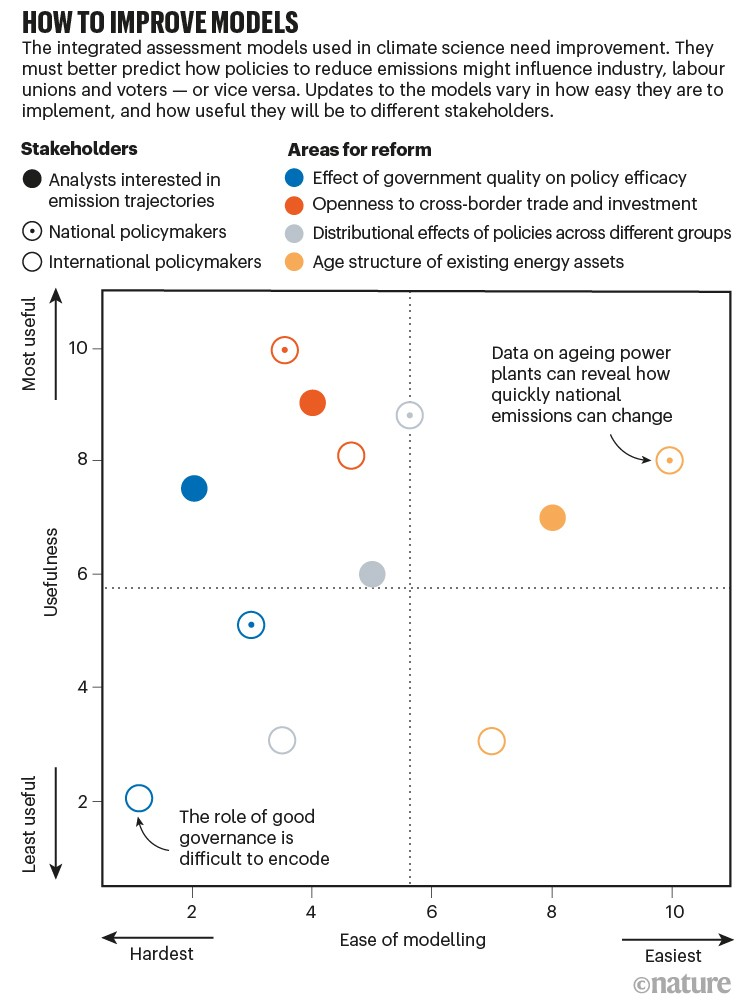
\includegraphics{fig/political_IAM.jpg}

\href{https://www.nature.com/articles/d41586-021-01500-2}{Peng (2021) Climate policy models need to get real about people --- here's how}

\hypertarget{coupled-climate-social-models}{%
\section{Coupled Climate-Social Models}\label{coupled-climate-social-models}}

\emph{Moore Abstract}

The ambition and effectiveness of climate policies will be essential in determining
greenhouse gas emissions and, as a consequence, the scale of climate change
impacts 1,2 . However, the socio-politico-technical processes that will determine
climate policy and emissions trajectories are treated as exogenous in almost all
climate change modelling 3,4 . Here we identify relevant feedback processes
documented across a range of disciplines and connect them in a stylized model of the
climate--social system. An analysis of model behaviour reveals the potential for
nonlinearities and tipping points that are particularly associated with connections
across the individual, community, national and global scales represented. These
connections can be decisive for determining policy and emissions outcomes. After
partly constraining the model parameter space using observations, we simulate
100,000 possible future policy and emissions trajectories. These fall into 5 clusters
with warming in 2100 ranging between 1.8 °C and 3.6 °C above the 1880--1910 average.
Public perceptions of climate change, the future cost and effectiveness of mitigation
technologies, and the responsiveness of political institutions emerge as important in
explaining variation in emissions pathways and therefore the constraints on warming
over the twenty-first century.

\emph{Moore Memo}

\href{https://www.nature.com/articles/s41586-022-04423-8}{Moore (2022) Determinants of emissions pathways in the
coupled climate--social system}
\href{pdf/Moore_2022_Coupled_Climate_Social.pdf}{(pdf)}

\href{https://www.volts.wtf/p/volts-podcast-fran-moore-on-how-to}{Volts Podcast: Fran Moore}

\hypertarget{dice-climate-model}{%
\section{DICE Climate Model}\label{dice-climate-model}}

\begin{quote}
If you enter the climatic conditions of Venus into the DICE integrated assessment model, the economy stills grows nicely and everyone lives happily ever after.
\end{quote}

Independent of the
normative assumptions of inequality aversion and time preferences,
the Paris agreement constitutes the economically optimal policy pathway
for the century.
Authors claim they show this by incorporating a
damage-cost curve reproducing
the observed relation between temperature
and economic growth into the integrated assessment model DICE.

\href{https://www.nature.com/articles/s41467-019-13961-1}{Glanemann (2021) DICE Paris CBA}
\href{pdf/Glanemann_2021_DICE_Paris_CBA.pdf}{(pdf)}

\hypertarget{the-failure-of-dice-economics}{%
\subsection{The failure of Dice Economics}\label{the-failure-of-dice-economics}}

If there is one climate economist who is respected above all others, it's William Nordhaus of Yale, who won the Econ Nobel in 2018 ``for integrating climate change into long-run macroeconomic analysis.'' The prize specifically cited Nordhaus' creation of an ``integrated assessment model'' for analyzing the costs of climate change. The most famous of these is the DICE Model, used by the Environmental Protection Agency.

But the DICE Model, or at least the version we've been using for years, is obviously bananas.

\href{https://noahpinion.substack.com/p/why-has-climate-economics-failed}{Noah Smith}

For other economists look here

\href{https://twitter.com/CatieHausman/status/1381999336423362568}{Catie Hausman Twitter Thread}

\hypertarget{e3me-ftt-genie}{%
\section{E3ME-FTT-GENIE}\label{e3me-ftt-genie}}

\emph{Mercure Abstract}

A high degree of consensus exists in the climate sciences over the role that human interference with the
atmosphere is playing in changing the climate. Following the Paris Agreement, a similar consensus exists
in the policy community over the urgency of policy solutions to the climate problem. The context for
climate policy is thus moving from agenda setting, which has now been mostly established, to impact
assessment, in which we identify policy pathways to implement the Paris Agreement. Most integrated
assessment models currently used to address the economic and technical feasibility of avoiding climate
change are based on engineering perspectives with a normative systems optimisation philosophy,
suitable for agenda setting, but unsuitable to assess the socio-economic impacts of realistic baskets of
climate policies. Here, we introduce a fully descriptive, simulation-based integrated assessment model
designed specifically to assess policies, formed by the combination of (1) a highly disaggregated macro-
econometric simulation of the global economy based on time series regressions (E3ME), (2) a family of
bottom-up evolutionary simulations of technology diffusion based on cross-sectional discrete choice
models (FTT), and (3) a carbon cycle and atmosphere circulation model of intermediate complexity
(GENIE). We use this combined model to create a detailed global and sectoral policy map and scenario
that sets the economy on a pathway that achieves the goals of the Paris Agreement with \textgreater66\% probability
of not exceeding 2 C of global warming. We propose a blueprint for a new role for integrated assessment
models in this upcoming policy assessment context.

\emph{Mecure Memo}

The E3ME-FTT-GENIE 2 model is a simulation-based integrated
assessment model that is fully descriptive, in which dynamical
(time-dependent) human or natural behaviour is driven by
empirically-determined dynamical relationships. At its core is the
macroeconomic model E3ME, which represents aggregate human
behaviour through a chosen set of econometric relationships that
are regressed on the past 45 years of data and are projected 35
years into the future. The macroeconomics in the model determine
total demand for manufactured products, services and energy car-
riers. Meanwhile, technology diffusion in the FTT family of tech-
nology modules determines changes in the environmental
intensity of economic processes, including changes in amounts of
energy required for transport, electricity generation and household
heating. Since the development and diffusion of new technologies
cannot be well modelled using time-series econometrics, cross-
sectional datasets are used to parameterise choice models in FTT.
Finally, greenhouse gas emissions are produced by the combustion
of fuels and by other industrial processes, which interfere with the
climate system. Natural non-renewable energy resources are
modelled in detail with a dynamical depletion algorithm. And
finally, to determine the climate impacts of chosen policies, E3ME-
FTT global emissions are fed to the GENIE carbon cycle-climate
system model of intermediate complexity. This enables, for
instance, policy-makers to determine probabilistically whether or
not climate targets are met.

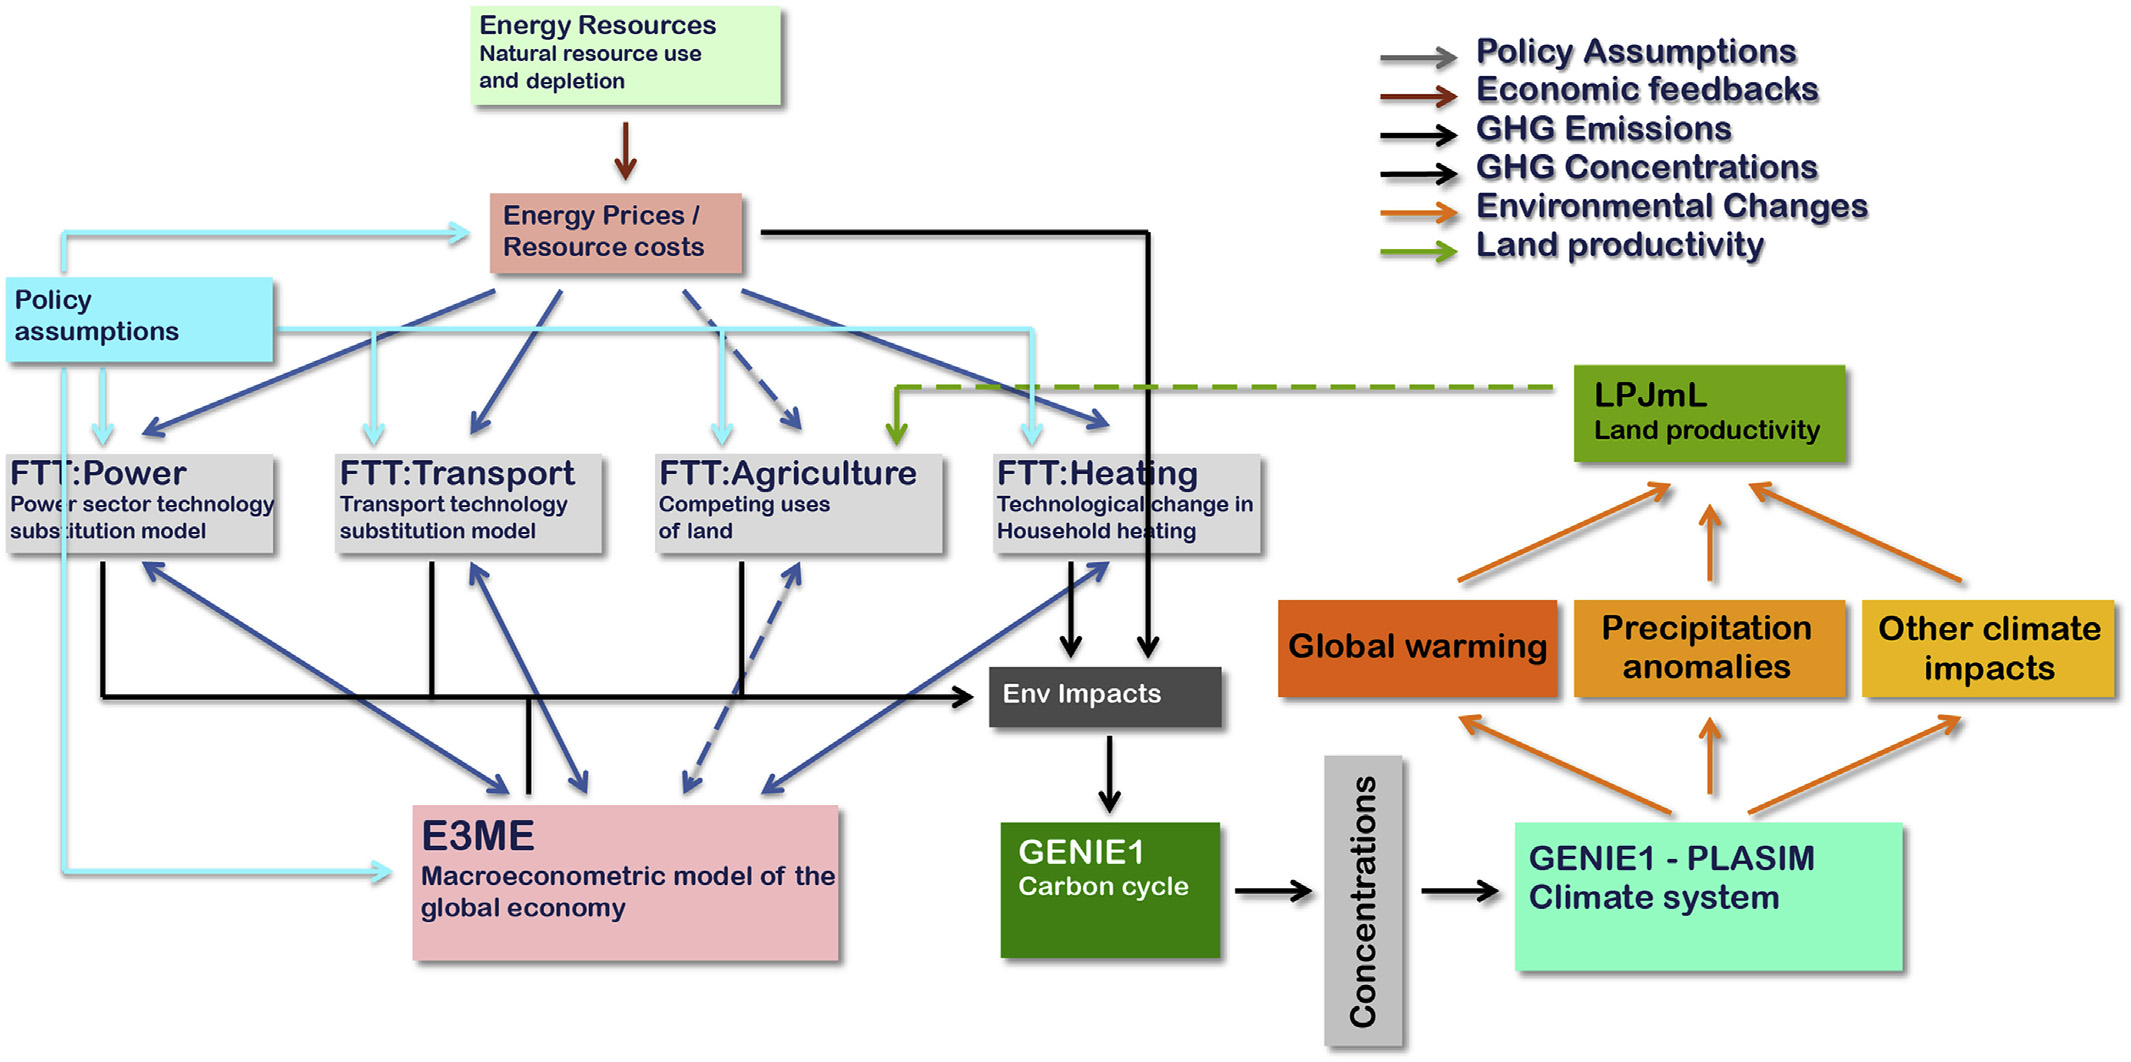
\includegraphics{fig/E3E-FTT-GENIE.png}

\href{https://www.sciencedirect.com/science/article/pii/S2211467X18300129?via\%3Dihub}{Mercure (2018) Environmental impact assessment for climate change policy with the simulation-based integrated assessment model E3ME-FTT-GENIE}
\href{pdf/Mercure_2018_E3ME-FTT-GENIE.pdf}{(pdf)}

\emph{Mercure Abstract}

A key aim of climate policy is to progressively substitute renewables and energy efficiency for fossil fuel use. The associated
rapid depreciation and replacement of fossil-fuel-related physical and natural capital entail a profound reorganization of indus-
try value chains, international trade and geopolitics. Here we present evidence confirming that the transformation of energy
systems is well under way, and we explore the economic and strategic implications of the emerging energy geography. We
show specifically that, given the economic implications of the ongoing energy transformation, the framing of climate policy as
economically detrimental to those pursuing it is a poor description of strategic incentives. Instead, a new climate policy incen-
tives configuration emerges in which fossil fuel importers are better off decarbonizing, competitive fossil fuel exporters are
better off flooding markets and uncompetitive fossil fuel producers---rather than benefitting from `free-riding'---suffer from
their exposure to stranded assets and lack of investment in decarbonization technologies.

\href{https://www.nature.com/articles/s41560-021-00934-2}{Mercure (2021) Reframing incentives for climate policy action}
\href{pdf/Mercure_2021_Reframing_incentives_for_Climate_Policy_Action.pdf}{(pdf)}

\hypertarget{ez-climate-model}{%
\section{EZ-Climate Model}\label{ez-climate-model}}

Some text on EZClimate

\hypertarget{fair-climate-model}{%
\section{FAIR Climate Model}\label{fair-climate-model}}

The FAIR model satisfies all
criteria set by the NAS for use in an SCC calculation. 22 Importantly, this model
generates projections of future warming that are consistent with comprehensive, state-
of-the-art models and it can be used to accurately characterize current best
understanding of the uncertainty regarding the impact that an additional ton of CO 2
has on global mean surface temperature (GMST). Finally, FAIR is easily implemented
and transparently documented, 23 and is already being used in updates of the SCC. 24

A key limitation of FAIR and other simple climate models is that they do not represent
the change in global mean sea level rise (GMSL) due to a marginal change in emissions.

\href{pdf/Greenstone_2021_Updating_SCC.pdf}{Carleton Greenstone (2021) Updating SCC (pdf)}

\href{https://fair.readthedocs.io/en/latest/}{FAIR}

\hypertarget{gcam}{%
\section{GCAM}\label{gcam}}

\emph{Global Change Analysis Model}

JGCRI is the home and primary development institution for the Global Change Analysis Model (GCAM), an integrated tool for exploring the dynamics of the coupled human-Earth system and the response of this system to global changes. GCAM is a global model that represents the behavior of, and interactions between five systems: the energy system, water, agriculture and land use, the economy, and the climate.

\href{http://www.globalchange.umd.edu/gcam/}{GCAM}

\href{https://github.com/JGCRI/gcam-core}{GCAM on GitHub}

\emph{GCAM Analysis of COP26 Pledges}

Over 100 nations have issued new commitments to reduce greenhouse gas emissions ahead of the United Nations Conference of the Parties, or COP26, currently underway in Glasgow.

A new analysis published today in the journal \href{https://www.science.org/doi/10.1126/science.abm1157}{Science} assessed those new pledges, or nationally determined commitments (NDCs), and how they could shape Earth's climate. The authors of the study, from institutions led by the Pacific Northwest National Laboratory and including Imperial College London, find the latest NDCs could chart a course where limiting global warming to 2°C and under within this century is now significantly more likely.

Under pledges made at the 2015 Paris Agreement, the chances of limiting temperature change to below 2°C and 1.5°C above the average temperature before the industrial revolution by 2100 were 8 and 0 per cent, respectively.

Under the new pledges -- if they are successfully fulfilled and reinforced with policies and measures of equal or greater ambition -- the study's authors estimate those chances now rise to 34 and 1.5 percent, respectively. If countries strike a more ambitious path beyond 2030, those probabilities become even more likely, rising to 60 and 11 percent, respectively.

Further, the chance of global temperatures rising above 4°C could be virtually eliminated. Under the 2015 pledges, the probability of such warming was more likely, at around 10 percent probability.

The researchers used an open-source model called the Global Change Analysis Model (GCAM) to simulate a spectrum of emissions scenarios.

\href{https://www.imperial.ac.uk/news/231739/new-climate-pledges-significantly-more-likely/}{Imperial College (2021) New climate pledges significantly more likely to prevent worst of global heating}

\emph{Dubash Abstract}

Discussions about climate mitigation tend to focus on the ambition of emission reduction targets or the prevalence, design, and stringency of climate policies. However, targets are more likely to translate to near-term action when backed by institutional machinery that guides policy development and implementation. Institutions also mediate the political interests that are often barriers to implementing targets and policies. Yet the study of domestic climate institutions is in its infancy, compared with the study of targets and policies. Existing governance literatures document the spread of climate laws (1, 2) and how climate policy-making depends on domestic political institutions (3--5). Yet these literatures shed less light on how states organize themselves internally to address climate change. To address this question, drawing on empirical case material summarized in table S1, we propose a systematic framework for the study of climate institutions. We lay out definitional categories for climate institutions, analyze how states address three core climate governance challenges---coordination, building consensus, and strategy development---and draw attention to how institutions and national political contexts influence and shape each other. Acontextual ``best practice'' notions of climate institutions are less useful than an understanding of how institutions evolve over time through interaction with national politics.

\href{https://www.science.org/doi/10.1126/science.abm1157}{Dubash (2021) National climate institutions complement targets and policies (Science)}

\hypertarget{global-calculator}{%
\section{Global Calculator}\label{global-calculator}}

Used by Kuhnhenn - STS - Heinrch Böll Stiftung

\href{http://www.globalcalculator.org/}{GlobalCalculator}

\href{http://tool.globalcalculator.org/globcalc.html?levers=22rfoe2e\%2013be1111c2c2c1n31hfjdcef222hp233f211111fn2211111111/dashboard/en}{Global Calculator Tool}

\hypertarget{modtran}{%
\chapter{MODTRAN}\label{modtran}}

\href{http://modtran.spectral.com/modtran_home\#plot}{MODTRAN Demo}

\emph{Benestad}

Kininmonth used MODTRAN, but he must show how MODTRAN was used to arrive at figures that differ from other calculations, which also use MODTRAN. It is an important principle in science that others can repeat the same calculations and arrive at the same answer. You can play with MODTRAN on its website, but it is still important to explain how you arrive at your answers.

\href{https://www.realclimate.org/index.php/archives/2022/10/new-misguided-interpretations-of-the-greenhouse-effect-from-william-kininmonth/}{Benestad(2022) ew misguided interpretations of the greenhouse effect from William Kininmonth}

\hypertarget{monash-climate-model}{%
\section{Monash Climate Model}\label{monash-climate-model}}

Some text on Monash Model

\hypertarget{page}{%
\section{PAGE}\label{page}}

\emph{Kikstra Abstract}

A key statistic describing climate change impacts is the `social cost of carbon dioxide' (SCCO 2 ), the
projected cost to society of releasing an additional tonne of CO 2 . Cost-benefit integrated
assessment models that estimate the SCCO 2 lack robust representations of climate feedbacks,
economy feedbacks, and climate extremes. We compare the PAGE-ICE model with the decade
older PAGE09 and find that PAGE-ICE yields SCCO 2 values about two times higher, because of its
climate and economic updates. Climate feedbacks only account for a relatively minor increase
compared to other updates. Extending PAGE-ICE with economy feedbacks demonstrates a
manifold increase in the SCCO 2 resulting from an empirically derived estimate of partially
persistent economic damages. Both the economy feedbacks and other increases since PAGE09 are
almost entirely due to higher damages in the Global South. Including an estimate of interannual
temperature variability increases the width of the SCCO 2 distribution, with particularly strong
effects in the tails and a slight increase in the mean SCCO 2 . Our results highlight the large impacts
of climate change if future adaptation does not exceed historical trends. Robust quantification of
climate-economy feedbacks and climate extremes are demonstrated to be essential for estimating
the SCCO 2 and its uncertainty.

\emph{Kikstra Memo}

How temperature rises affect long-run economic
output is an important open question (Piontek et al
2021). Climate impacts could either trigger addi-
tional GDP growth due to increased agricultural
productivity and rebuilding activities (Stern 2007,
Hallegatte and Dumas 2009, Hsiang 2010, National
Academies of Sciences Engineering and Medicine
2017) or inhibit growth due to damaged capital
stocks (Pindyck 2013), lower savings (Fankhauser and
Tol 2005) and inefficient factor reallocation (Piontek
et al 2019). Existing studies have identified substan-
tial impacts of economic growth feedbacks (Moyer
et al 2014, Dietz and Stern 2015, Estrada et al 2015,
Moore and Diaz 2015), but have not yet quantified
the uncertainties involved based on empirical distri-
butions. One particular example is Kalkuhl and Wenz
(2020), who incorporate short-term economic per-
sistence into a recent version of DICE (Nordhaus
2017), approximately tripling the resulting SCCO 2
(\$37--\$132). For fairly comparable economic assump-
tions, the effect of long-term persistence is shown to
increase the outcome even more (\$220--\$417) (Moore
and Diaz 2015, Ricke et al 2018). We further expand
on this work by deriving an empirical distribution
of the persistence of climate impacts on economic
growth based on recent developments (Burke et al
2015, Bastien-Olvera and Moore 2021) which we use
to moderate GDP growth through persistent market
damages. This partial persistence model builds upon
recent empirical insights that not all contemporary
economic damages due to climate change might be
recovered in the long run (Dell et al 2012, Burke
et al 2015, Kahn et al 2019, Bastien-Olvera and Moore
2021). Investigating how the SCCO 2 varies as a func-
tion of the extent of persistence reveals a sensitivity
that is on par with the heavily discussed role of dis-
counting (Anthoff et al 2009b).

Climatic extremes are another particularly
important driver of climate change-induced dam-
ages (Field et al 2012, Kotz et al 2021). The impact
of interannual climate variability on the SCCO 2 has,
however, not been analyzed previously, despite its
clear economic implications (Burke et al 2015, Kahn
et al 2019, Kumar and Khanna 2019) and an appar-
ent relation to weather extremes such as daily min-
ima and maxima (Seneviratne et al 2012), extreme
rainfall (Jones et al 2013), and floods (Marsh et al
2016). Omission of such features in climate-economy
models risks underestimation of the SCCO 2 because
if convex regional temperature damage functions
(Burke et al 2015) and an expected earlier cross-
ing of potential climate and social thresholds in
the climate-economy system (Tol 2019, Glanemann
et al 2020). Here, we include climate variability by
coupling the empirical temperature-damage func-
tion with variable, autoregressive interannual tem-
peratures. Increasing the amount of uncertainty by
adding variable elements naturally leads to a less con-
strained estimate for climate-driven impacts. How-
ever, it is important to explore the range of possible
futures, including the consideration of extremes in
the climate-economy system (Otto et al 2020).
In summary, we extend the PAGE-ICE CB-IAM
(Yumashev et al 2019) to quantify the effect on
the SCCO 2 of including possible long-term tem-
perature growth feedback on economic trajectories,
mean annual temperature anomalies, and the already
modeled permafrost carbon and surface albedo feed-
backs. Together, these provide an indication of the
magnitude and uncertainties of the contribution of
climate and economy feedbacks and interannual vari-
ability to the SCCO 2 .

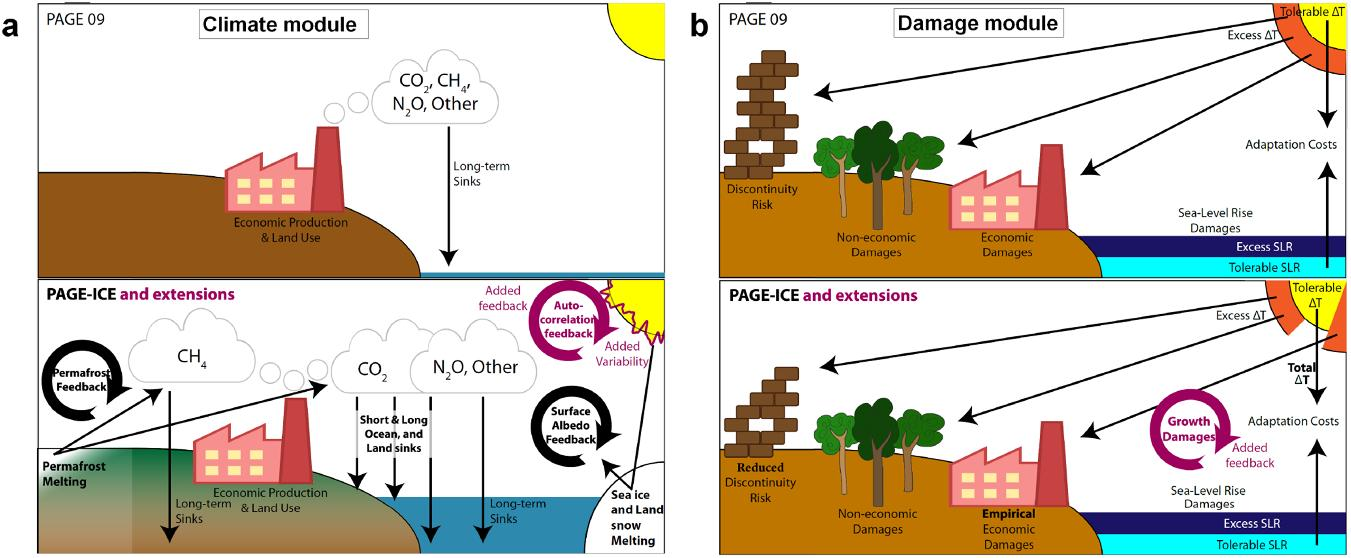
\includegraphics{fig/PAGE-ICE-extensions.jpg}

\emph{Figure: Illustrative sketch of changes and extensions to PAGE-ICE presented in this paper. (a) Changes in the climate
representation. PAGE-ICE includes a more detailed representation of CO 2 and CH 4 sinks, permafrost carbon feedback, the effect
of sea ice and land snow decline on surface albedo, and a fat-tailed distribution of sea level rise. Here we also include interannual
temperature variability with a temperature feedback through annual auto-correlation. (b) Changes in the damage module. The
PAGE-ICE discontinuity damage component was reduced to correspond with updates to climate tipping points and sea-level rise
risk, and market damages were recalibrated to an empirical estimate based on temperatures. Thus, while the discontinuity and
non-economic damages continue to be calculated based on the separation between tolerable and excess temperature, the market
damages are now calculated based on absolute temperature. Here we also extend PAGE-ICE with the possibility of persistent
climate-induced damages, which in turn affects GDP pathways and scales emissions accordingly (feedback loop in the figure).}

The original PAGE-
ICE does not simulate damage persistence. Thus, the
economy always returns to the exogenous economic
growth path, no matter how high the contemporary
damages.

Our setup recognizes that deterministic assessments
of the SCCO 2 carry only very limited information.
PAGE-ICE uses Monte Carlo sampling of over 150
parameter distributions (Yumashev et al 2019) to
provide distributions of the results. All results presen-
ted use 50 000 Monte Carlo draws (and 100 000 for
PAGE09, using \citet{RISK} within Excel), with draws
taken from the same superset to be able to compare
SCCO 2 distributions across models. The PAGE-ICE
model has been translated into the Mimi mod-
eling framework, using the same validation pro-
cess as for Mimi-PAGE (Moore et al 2018). Model
code and documentation are available from the
GitHub repository, \href{https://github.com/openmodels/MimiPAGE2020.jl}{here}.

To estimate the marginal damage of an additional
tonne of CO 2 , PAGE-ICE is run twice, with one run
following the exogenously specified emission pathway
and the second run adding a CO 2 pulse. The SCCO 2
is then calculated as the difference in global equity-
weighted damages between those two runs divided
by the pulse size, discounted to the base year (2015).
Equity weighting of damages follows the approach
by Anthoff et al (2009a) using a mean (minimum,
maximum) elasticity of marginal utility of consump-
tion of 1.17 (0.1--2.0), and equity-weighted damages
are discounted using a pure time preference rate of
1.03\% (0.5\%, 2.0\%). For all our results, we rely on
a 75Gt pulse size in the first time period of PAGE-
ICE (mid-2017--2025), representing an annual pulse
size of 10 Gt CO 2 . In this setup, we found that
the choice of pulse size can have an effect on the
SCCO 2 estimates.

We implement the persistence parameter following
Estrada et al (2015) into the growth system of Burke
et al (2015) such that:
\[GDP_{r , t} = GDP_{r , t − 1} · (1 + g_{r , t − ρ} · γ_{r , t − 1} )\],
where g is the growth rate, γ represents
the contemporary economic damages in \% of GDP
returned by the market damage function and ρ specifies
the share of economic damages that persist and
thus alter the growth trajectory in the long run. Note
that this approach nests the extreme assumptions
of zero persistence usually made in CB-IAMs.
We also rescale green-house gas emissions proportionally to the change in
GDP, such that emission intensities of economic output remain unchanged.

\emph{Kikstra Conclusions}

Our results show that determining the level of per-
sistence of economic damages is one of the most
important factors in calculating the SCCO 2 , and our
empirical estimate illustrates the urgency of increas-
ing adaptive capacity, while suggesting that the mean
estimate for the SCCO 2 may have been strongly
underestimated. It further indicates that considering
annual temperature anomalies leads to large increases
in uncertainty about the risks of climate change.
Differences between PAGE09 and PAGE-ICE show
that the previous SCCO 2 results have also decidedly
underestimated damages in the Global South.
The implemented climate feedbacks and annual
mean temperature variability do not have large effects
on the mean SCCO 2 . The inclusion of permafrost
thawing and surface albedo feedbacks is shown to lead
to a relatively small increase in the SCCO 2 for SSP2-
4.5, with modest distributional effects. Consideration
of temperature anomalies shows that internal vari-
ability in the climate system can lead to increases in
SCCO 2 estimates, and is key to understanding uncer-
tainties in the climate-economy system, stressing the
need for a better representation of variability and
extremes in CB-IAMs.
Including an empirical estimate of damage per-
sistence demonstrates that even minor departures
from the assumption that climate shocks do not affect
GDP growth have major economic implications and
eclipse most other modeling decisions. It suggests
the need for a strong increase in adaptation to per-
sistent damages if the long-term social cost of emis-
sions is to be limited. Our findings corroborate that
economic uncertainty is larger than climate science
uncertainty in climate-economy system analysis (Van
Vuuren et al 2020), and provide a strong argument
that the assumption of zero persistence in CB-IAMs
should be subject to increased scrutiny in order to
avoid considerable bias in SCCO 2 estimates.

\href{https://iopscience.iop.org/article/10.1088/1748-9326/ac1d0b}{Kikstra (2021) The social cost of carbon dioxide under climate-economy feedbacks and temperature variability}
\href{pdf/Kikstra_2021_SSC_Climate_Economy_Feedbacks_PAGE.pdf}{(pdf)}

\emph{MIMI Modelling Framwork}

Mimi is a Julia package for integrated assessment models developed in connection with Resources for the Future's Social Cost of Carbon Initiative.
The source code for this package is located on Github \href{https://github.com/mimiframework/Mimi.jl}{here}, and for detailed information on the installation and use of this package, as well as several tutorials, please see the \href{https://www.mimiframework.org/Mimi.jl/stable/}{Documentation}. For specific requests for new functionality, or bug reports, please add an Issue to the repository.

\href{https://www.mimiframework.org/}{MIMI Home Page}

\emph{Kikstra Review}

\href{https://www.sueddeutsche.de/wissen/hochwasserkatastrophe-schaeden-kosten-klimawandel-co2-preis-hurrikan-1.5402770}{Süd-Deutsche}

\hypertarget{bern-simple-climate-model-bernscm}{%
\section{Bern Simple Climate Model (BernSCM)}\label{bern-simple-climate-model-bernscm}}

\emph{Bern SCM Github README.md}

The Bern Simple Climate Model (BernSCM) is a free open source reimplementation of a reduced form carbon cycle-climate model which has been used widely in previous scientific work and IPCC assessments.
BernSCM represents the carbon cycle and climate system with a small set of equations for the heat and carbon budget, the parametrization of major nonlinearities, and the substitution of complex component systems with impulse response functions (IRF). The IRF approach allows cost-efficient yet accurate substitution of detailed parent models of climate system components with near linear behaviour. Illustrative simulations of scenarios from previous multi-model studies show that BernSCM is broadly representative of the range of the climate-carbon cycle response simulated by more complex and detailed models. Model code (in Fortran) was written from scratch with transparency and extensibility in mind, and is provided as open source. BernSCM makes scientifically sound carbon cycle-climate modeling available for many applications. Supporting up to decadal timesteps with high accuracy, it is suitable for studies with high computational load, and for coupling with, e.g., Integrated Assessment Models (IAM). Further applications include climate risk assessment in a business, public, or educational context, and the estimation of CO2 and climate benefits of emission mitigation options.

See the file BernSCM\_manual(.pdf) for instructions on the use of the program.

\href{https://www.researchgate.net/publication/320808211_The_Bern_Simple_Climate_Model_BernSCM_v10_an_extensible_and_fully_documented_open_source_reimplementation_of_the_Bern_reduced_form_model_for_global_carbon_cycle-climate_simulations}{Strassmann 2017 The BernSCM}
\href{https://doi.org/10.5281/zenodo.1038117}{Bern SCM}
\href{pdf/Strassmann_2017_BernSCM.pdf}{(pdf)}
\href{https://github.com/bernSCM/bernSCM}{Bern SCM Github Code}

\emph{Parameters for tuning Bern}

\href{https://unfccc.int/resource/brazil/carbon.html}{UNFCCC}

\textbf{Critics of Bern Model}

Y'know, it's hard to figure out what the Bern model says about anything. This is because, as far as I can see, the Bern model proposes an impossibility. It says that the CO2 in the air is somehow partitioned, and that the different partitions are sequestered at different rates.

For example, in the IPCC Second Assessment Report (SAR), the atmospheric CO2 was divided into six partitions, containing respectively 14\%, 13\%, 19\%, 25\%, 21\%, and 8\% of the atmospheric CO2.

Each of these partitions is said to decay at different rates given by a characteristic time constant ``tau'' in years. (See Appendix for definitions). The first partition is said to be sequestered immediately. For the SAR, the ``tau'' time constant values for the five other partitions were taken to be 371.6 years, 55.7 years, 17.01 years, 4.16 years, and 1.33 years respectively.

Now let me stop here to discuss, not the numbers, but the underlying concept. The part of the Bern model that I've never understood is, what is the physical mechanism that is partitioning the CO2 so that some of it is sequestered quickly, and some is sequestered slowly?

I don't get how that is supposed to work. The reference given above says:

CO2 concentration approximation

The CO2 concentration is approximated by a sum of exponentially decaying functions, one for each fraction of the additional concentrations, which should reflect the time scales of different sinks.

So theoretically, the different time constants (ranging from 371.6 years down to 1.33 years) are supposed to represent the different sinks. Here's a graphic showing those sinks, along with approximations of the storage in each of the sinks as well as the fluxes in and out of the sinks:

(Carbon Cycle Picture)

Now, I understand that some of those sinks will operate quite quickly, and some will operate much more slowly.

But the Bern model reminds me of the old joke about the thermos bottle (Dewar flask), that poses this question:

The thermos bottle keeps cold things cold, and hot things hot \ldots{} but how does it know the difference?

So my question is, how do the sinks know the difference?

Why don't the fast-acting sinks just soak up the excess CO2, leaving nothing for the long-term, slow-acting sinks? I mean, if some 13\% of the CO2 excess is supposed to hang around in the atmosphere for 371.3 years \ldots{} how do the fast-acting sinks know to not just absorb it before the slow sinks get to it?

Anyhow, that's my problem with the Bern model---I can't figure out how it is supposed to work physically.

Finally, note that there is no experimental evidence that will allow us to distinguish between plain old exponential decay (which is what I would expect) and the complexities of the Bern model. We simply don't have enough years of accurate data to distinguish between the two.

Nor do we have any kind of evidence to distinguish between the various sets of parameters used in the Bern Model. As I mentioned above, in the IPCC SAR they used five time constants ranging from 1.33 years to 371.6 years (gotta love the accuracy, to six-tenths of a year).

But in the IPCC Third Assessment Report (TAR), they used only three constants, and those ranged from 2.57 years to 171 years.

However, there is nothing that I know of that allows us to establish any of those numbers. Once again, it seems to me that the authors are just picking parameters.

So \ldots{} does anyone understand how 13\% of the atmospheric CO2 is supposed to hang around for 371.6 years without being sequestered by the faster sinks?

All ideas welcome, I have no answers at all for this one. I'll return to the observational evidence regarding the question of whether the global CO2 sinks are ``rapidly diminishing'', and how I calculate the e-folding time of CO2 in a future post.

Best to all,

\begin{enumerate}
\def\labelenumi{\alph{enumi}.}
\setcounter{enumi}{22}
\tightlist
\item
\end{enumerate}

APPENDIX: Many people confuse two ideas, the residence time of CO2, and the ``e-folding time'' of a pulse of CO2 emitted to the atmosphere.

The residence time is how long a typical CO2 molecule stays in the atmosphere. We can get an approximate answer from Figure 2. If the atmosphere contains 750 gigatonnes of carbon (GtC), and about 220 GtC are added each year (and removed each year), then the average residence time of a molecule of carbon is something on the order of four years. Of course those numbers are only approximations, but that's the order of magnitude.

The ``e-folding time'' of a pulse, on the other hand, which they call ``tau'' or the time constant, is how long it would take for the atmospheric CO2 levels to drop to 1/e (37\%) of the atmospheric CO2 level after the addition of a pulse of CO2. It's like the ``half-life'', the time it takes for something radioactive to decay to half its original value. The e-folding time is what the Bern Model is supposed to calculate. The IPCC, using the Bern Model, says that the e-folding time ranges from 50 to 200 years.

On the other hand, assuming normal exponential decay, I calculate the e-folding time to be about 35 years or so based on the evolution of the atmospheric concentration given the known rates of emission of CO2. Again, this is perforce an approximation because few of the numbers involved in the calculation are known to high accuracy. However, my calculations are generally confirmed by those of Mark Jacobson as published \href{http://www.stanford.edu/group/efmh/jacobson/Articles/VIII/fossil/ClimRespUpdJGR\%201.pdf}{here} in the Journal of Geophysical Research.

\href{https://climateilluminated.com/CO2_facts/carbon_cycle/CO2_residence_Bern_model.html}{Eschenbach}

\textbf{CO2 Lifetime}

The overall lifetime of CO 2 is updated to range from 30 to 95 years

Any emission reduction of fossil-fuel particulate BC {[}Black Carbon{]} plus
associated OM {[}Organic Matter{]} may slow global warming more
than may any emission reduction of CO 2 or CH 4 for a specific period,

\emph{Jacobsen Abstract}

This document describes two updates and a correction that affect two figures
(Figures 1 and 14) in ``Control of fossil-fuel particulate black carbon and organic matter,
possibly the most effective method of slowing global warming'' by Mark Z. Jacobson
(Journal of Geophysical Research, 107(D19), 4410, \url{doi:10.1029/2001JD001376}, 2002).
The modifications have no effect on the numerical simulations in the paper, only on the
postsimulation analysis. The changes include the following: (1) The overall lifetime of
CO 2 is updated to range from 30 to 95 years instead of 50 to 200 years, (2) the
assumption that the anthropogenic emission rate of CO 2 is in equilibrium with its
atmospheric mixing ratio is corrected, and (3) data for high-mileage vehicles available in
the U.S. are used to update the range of mileage differences (15--30\% better for diesel) in
comparison with one difference previously (30\% better mileage for diesel). The
modifications do not change the main conclusions in J2002, namely, (1) ``any emission
reduction of fossil-fuel particulate BC plus associated OM may slow global warming more
than may any emission reduction of CO 2 or CH 4 for a specific period,'' and (2) diesel
cars emitting continuously under the most recent U.S. and E.U. particulate standards
(0.08 g/mi; 0.05 g/km) may warm climate per distance driven over the next 100+ years
more than equivalent gasoline cars. Toughening vehicle particulate emission standards by
a factor of 8 (0.01 g/mi; 0.006 g/km) does not change this conclusion, although it
shortens the period over which diesel cars warm to 13--54 years,'\,' except as follows: for
conclusion 1, the period in Figure 1 of J2002 during which eliminating all fossil-fuel
black carbon plus organic matter (f.f. BC + OM) has an advantage over all anthropogenic
CO 2 decreases from 25--100 years to about 11--13 years and for conclusion 2 the period in
Figure 14 of J2002 during which gasoline vehicles may have an advantage broadens
from 13 to 54 years to 10 to \textgreater100 years. On the basis of the revised analysis, the ratio of
the 100-year climate response per unit mass emission of f.f. BC + OM relative to that of
CO 2 -C is estimated to be about 90--190.

\href{http://www.stanford.edu/group/efmh/jacobson/Articles/VIII/fossil/ClimRespUpdJGR\%201.pdf}{Jacobsen (2002)}
\href{pdf/Jacobsen_2002_CO2_Lifetime.pdf}{(pdf)}

\emph{What's Up with the Bern Model}

\emph{Mearns}

In modelling the growth of CO2 in the atmosphere from emissions data it is standard practice to model what remains in the atmosphere since after all it is the residual CO2 that is of concern in climate studies. In this post I turn that approach on its head and look at what is sequestered. This gives a very different picture showing that the Bern T1.2 and T18.5 time constants account for virtually all of the sequestration of CO2 from the atmosphere on human timescales (see chart below). The much longer T173 and T∞ processes are doing virtually nothing. Their principle action is to remove CO2 from the fast sinks, not from the atmosphere, in a two stage process that should not be modelled as a single stage. Given time, the slow sinks will eventually sequester 100\% of human emissions and not 48\% as the Bern model implies.

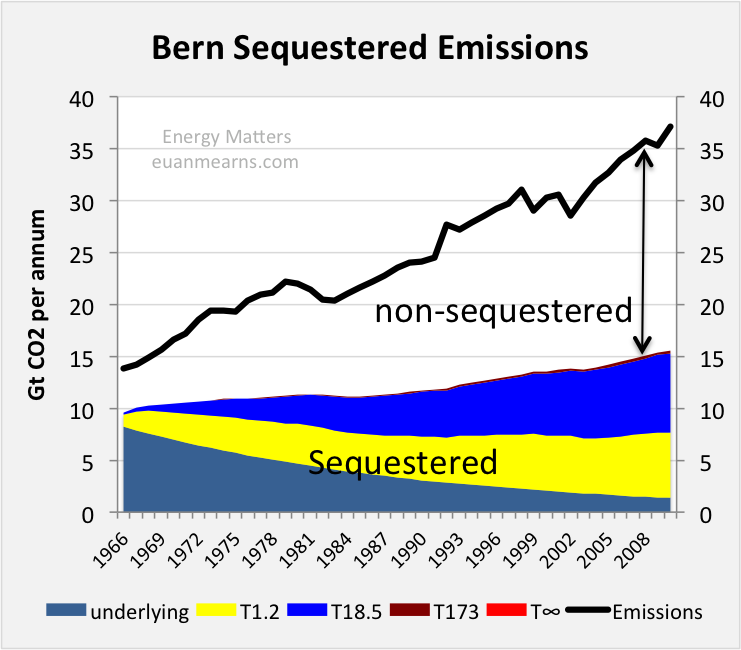
\includegraphics{fig/bern_sequestered.png}

\emph{Figure: The chart shows the amount of annual emissions removed by the various components of the Bern model. Unsurprisingly the T∞ component with a decline rate of 0\% removes zero emissions and the T173 slow sink is not much better. Arguably, these components should not be in the model at all. The fast T1.2 and T18.5 sinks are doing all the work. The model does not handle the pre-1965 emissions decline perfectly, shown as underlying, but these too will be removed by the fast sinks and should also be coloured yellow and blue. Note that year on year the amount of CO2 removed has risen as partial P of CO2 has gone up. The gap between the coloured slices and the black line is that portion of emissions that remained in the atmosphere.}

The Bern Model for sequestration of CO2 from Earth's atmosphere imagines the participation of a multitude of processes that are summarised into four time constants of 1.2, 18.5 and 173 years and one constant with infinity (Figure 1). I described it at length in this earlier post \href{http://euanmearns.com/?p=4490}{The Half Life of CO2 in Earth's Atmosphere}.

\href{https://euanmearns.com/whats-up-with-the-bern-model/}{Mearns}

\hypertarget{noresm}{%
\section{NorESM}\label{noresm}}

\textbf{Norwegian Earth System Model}

\emph{About}

A climate model solves mathematically formulated natural laws on a three-dimensional grid. The climate model divides the soil system into components (atmosphere, sea, sea ice, land with vegetation, etc.) that interact through transmission of energy, motion and moisture. When the climate model also includes advanced interactive atmosphere chemistry and biogeochemical cycles (such as the carbon cycle), it is called an earth system model.

The Norwegian Earth System Model NorESM has been developed since 2007 and has been an important tool for Norwegian climate researchers in the study of the past, present and future climate. NorESM has also contributed to climate simulation that has been used in research assessed in the IPCC's fifth main report.

\emph{INES}

The project Infrastructure for Norwegian Earth System Modeling (INES) will support the further development of NorESM and help Norwegian scientists also gain access to a cutting-edge earth system model in the years to come. Technical support will be provided for the use of a more refined grid, the ability to respond to climate change up to 10 years in advance, the inclusion of new processes at high latitudes and the ability of long-term projection of sea level.
Climate simulations with NorESM are made on some of the most powerful supercomputers in Norway, and INES will help these exotic computers to be exploited in the best possible way and that the large data sets produced are efficiently stored and used. The project will ensure that researchers can efficiently use the model tool, analyze results and make the results available.

\hypertarget{ccsm4}{%
\subsection{CCSM4}\label{ccsm4}}

\emph{UCAR NCAR}

The University Corporation for Atmospheric Research (UCAR) is a
US nonprofit consortium of more than 100 colleges and universities providing
research and training in the atmospheric and related sciences.
UCAR manages the National Center for Atmospheric Research (NCAR) and
provides additional services to strengthen and support research and education
through its community programs.
Its headquarters, in Boulder, Colorado, include NCAR's Mesa Laboratory. (Wikipedia)

\emph{CCSM}

The Community Climate System Model (CCSM) is a
coupled climate model for simulating Earth's climate system.
CCSM consists of five geophysical models:
atmosphere (atm), sea-ice (ice), land (lnd), ocean (ocn), and land-ice (glc),
plus a coupler (cpl) that coordinates the models and passes information between them.
Each model may have ``active,'' ``data,'' ``dead,'' or ``stub'' component version allowing
for a variety of ``plug and play'' combinations.

During the course of a CCSM run, the model components integrate forward in time, periodically stopping to exchange information with the coupler. The coupler meanwhile receives fields from the component models, computes, maps, and merges this information, then sends the fields back to the component models. The coupler brokers this sequence of communication interchanges and manages the overall time progression of the coupled system. A CCSM component set is comprised of six components: one component from each model (atm, lnd, ocn, ice, and glc) plus the coupler. Model components are written primarily in Fortran 90.

\href{https://www.cesm.ucar.edu/models/ccsm4.0/ccsm_doc/x42.html\#ccsm_machines}{ccsm4}

\emph{CESM}

The Community Earth System Model (CESM) is a fully-coupled, global climate model that provides state-of-the-art computer simulations of the Earth's past, present, and future climate states.

CESM2 is the most current release and contains support for CMIP6 experiment configurations.

\href{https://www.cesm.ucar.edu/models/}{cesm models}

\emph{Simpler Models}

As part of CESM2.0, several dynamical core and aquaplanet configurations have been made available.

\href{https://www.cesm.ucar.edu/models/simpler-models/}{Simpler Models}

\hypertarget{noresm-features}{%
\subsection{NorESM Features}\label{noresm-features}}

Despite the nationally coordinated effort, Norway has
insufficient expertise and manpower to develop, test, verify
and maintain a complete earth system model. For this reason,
NorESM is based on the Community Climate System Model version 4,
CCSM4, operated at the National Center for
Atmospheric Research on behalf of the Community Climate
System Model (CCSM)/Community Earth System Model
(CESM) project of the University Corporation for
Atmospheric Research.

NorESM is, however, more than a model
``dialect'' of CCSM4. Notably, NorESM differs from CCSM4
in the following aspects: NorESM utilises an isopycnic
coordinate ocean general circulation model developed in
Bergen during the last decade originating from the Miami Isopycnic Coordinate
Ocean Model (MICOM). The atmospheric module is modified with
chemistry--aerosol--cloud--radiation interaction schemes developed for the Oslo
version of the Community Atmosphere Model (CAM4-Oslo).
Finally, the HAMburg Ocean Carbon Cycle (HAMOCC) model developed at the Max Planck
Institute for Meteorology, Hamburg, adapted to an isopycnic ocean
model framework, constitutes the core of
the biogeochemical ocean module in NorESM.
In this way NorESM adds to the much desired climate model diversity,
and thus to the hierarchy of models participating in phase
5 of the Climate Model Intercomparison Project (CMIP5).
In this and in an accompanying paper (Iversen et al., 2013), NorESM without
biogeochemical cycling is presented.
The reader is referred to Assmann et al.~(2010) and Tjiputra et al.~(2013)
for a description of the biogeochemical ocean component and carbon
cycle version of NorESM, respectively.

There are several overarching objectives underlying the
development of NorESM. Western Scandinavia and the surrounding
seas are located in the midst of the largest surface
temperature anomaly on earth governed
by anomalously large oceanic and atmospheric heat
transports.
Small changes to these transports may result in large and abrupt changes in the local climate.
To better understand the variability and stability of the climate system,
detailed studies of the formation, propagation
and decay of thermal and (oceanic) fresh water anomalies are required.

NorESM is, as mentioned above, largely based on CCSM4.
The main differences are the isopycnic coordinate ocean
module in NorESM and that CAM4-Oslo substitutes CAM4
as the atmosphere module. The sea ice and land models in
NorESM are basically the same as in CCSM4 and the Com-
munity Earth System Model version 1 (CESM1), except that
deposited soot and mineral dust aerosols on snow and sea ice
are based on the aerosol calculations in CAM4-Oslo.

\hypertarget{noresm-aerosol-interactions}{%
\subsubsection{NorESM Aerosol Interactions}\label{noresm-aerosol-interactions}}

The aerosol module is extended from earlier versions that
have been published, and includes life-cycling of sea salt,
mineral dust, particulate sulphate, black carbon, and primary
and secondary organics. The impacts of most of the numer-
ous changes since previous versions are thoroughly explored
by sensitivity experiments. The most important changes are:
modified prognostic sea salt emissions; updated treatment
of precipitation scavenging and gravitational settling; inclu-
sion of biogenic primary organics and methane sulphonic
acid (MSA) from oceans; almost doubled production of land-
based biogenic secondary organic aerosols (SOA); and in-
creased ratio of organic matter to organic carbon (OM/OC)
for biomass burning aerosols from 1.4 to 2.6.
Compared with in situ measurements and remotely sensed
data, the new treatments of sea salt and dust aerosols
give smaller biases in near-surface mass concentrations and
aerosol optical depth than in the earlier model version. The
model biases for mass concentrations are approximately un-
changed for sulphate and BC. The enhanced levels of mod-
led OM yield improved overall statistics, even though OM
is still underestimated in Europe and overestimated in North
America.
The global anthropogenic aerosol direct radiative forc-
ing (DRF) at the top of the atmosphere has changed from
a small positive value to −0.08 W m −2 in CAM4-Oslo. The
sensitivity tests suggest that this change can be attributed to
the new treatment of biomass burning aerosols and gravita-
tional settling. Although it has not been a goal in this study,
the new DRF estimate is closer both to the median model
estimate from the AeroCom intercomparison and the best es-
timate in IPCC AR4. Estimated DRF at the ground surface
has increased by ca. 60 \%, to −1.89 W m −2

The increased abundance of natural OM and the introduc-
tion of a cloud droplet spectral dispersion formulation are the
most important contributions to a considerably decreased es-
timate of the indirect radiative forcing (IndRF). The IndRF
is also found to be sensitive to assumptions about the coat-
ing of insoluble aerosols by sulphate and OM. The IndRF of
−1.2 W m −2 , which is closer to the IPCC AR4 estimates than
the previous estimate of −1.9 W m −2 , has thus been obtained
without imposing unrealistic artificial lower bounds on cloud
droplet number concentrations.

\href{https://www.noresm.org/}{NorESM}

\href{https://gmd.copernicus.org/articles/6/687/2013/}{Bentsen (2013) NorESM - Part 1}
\href{pdf/Bentsen_2013_NorESM_1.pdf}{(pdf)}

\href{https://gmd.copernicus.org/articles/6/389/2013/}{Iversen (2013) NorESM - Part 2}
\href{pdf/Iversen_2013_NorESM_2.pdf}{(pdf)}

\href{https://gmd.copernicus.org/articles/3/143/2010/}{Assmann (2010) Biogeochemical Ocean Component - Isopycnic}
\href{pdf/Assmann_2010_Isopycnic_Ocean_Carbon_Cycle_Model.pdf}{(pdf)}

\href{https://gmd.copernicus.org/articles/3/123/2010/}{Tjiputra (2010) Carbon Cycle Component}
\href{pdf/Tjiputra_2010_Climate_Cycle_Feedbacks.pdf}{(pdf)}

\href{https://gmd.copernicus.org/articles/6/207/2013/}{Kirkevaag (2013) Aerosol-Climate Interactions}
\href{pdf/Kirkevaag_2013_Aerosol_NorESM.pdf}{(pdf)}

\href{https://www.cesm.ucar.edu/}{Community Earth System Model CESM}

\hypertarget{ai-in-climate-research}{%
\section{AI in Climate Research}\label{ai-in-climate-research}}

\emph{Irrgang Abstract}

Earth system models (ESMs) are our main tools for quantifying the physical state of the Earth and predicting how it might change in the future under ongoing anthropogenic forcing. In recent years, however, artificial intelligence (AI) methods have been increasingly used to augment or even replace classical ESM tasks, raising hopes that AI could solve some of the grand challenges of climate science. In this Perspective we survey the recent achievements and limitations of both process-based models and AI in Earth system and climate research, and propose a methodological transformation in which deep neural networks and ESMs are dismantled as individual approaches and reassembled as learning, self-validating and interpretable ESM--network hybrids. Following this path, we coin the term neural Earth system modelling. We examine the concurrent potential and pitfalls of neural Earth system modelling and discuss the open question of whether AI can bolster ESMs or even ultimately render them obsolete.

\href{https://www.nature.com/articles/s42256-021-00374-3}{Irrgang (2021) Towards neural Earth system modelling by integrating artificial intelligence in Earth system science (paywall)}

\emph{CarbonBrief}

A new line of climate research is emerging that aims to complement and extend the use of observations and climate models.
We propose an approach whereby machine learning and climate models are not used as individual tools, but rather as connected ``hybrids'' that are capable of adaptive evolution and self-validation, while still being able to be interpreted by humans.

Climate models have seen continuous improvement over recent decades. The most recent developments have seen the incorporation of biogeochemical cycles -- the transfer of chemicals between living things and their environment -- and how they interact with the climate system.
Adding in new processes and greater detail have resulted in more sophisticated simulations of the Earth's climate, it comes at the cost of increasingly large and complex models.

ESMs are built on equations that represent the processes and interactions that drive the Earth's climate. Some of these processes can be described by fundamental laws -- such as the Navier-Stokes equations of fluid motion, which capture the speed, pressure, temperature and density of the gases in the atmosphere and the water in the ocean. However, others -- such as physiological processes governing the vegetation that covers vast parts of the land surface -- cannot and instead require approximations based on observations.

These approximations -- as well as other limitations that stem from the sheer complexity of the Earth system -- introduce uncertainties into the model's representation of the climate.

As a result, despite the tremendous success of ESMs, some limitations remain -- such as how well models capture the severity and frequency of extreme events, and abrupt changes and ``tipping points''.

In contrast to ESMs, machine learning does not require prior knowledge about the governing laws and relations within a problem. The respective relations are derived entirely from the data used during an automated learning process. This flexible and powerful concept can be expanded to almost any level of complexity.

The availability of observed climate data and model simulations in combination with ready-to-use machine learning tools -- such as TensorFlow and Keras -- have led to an explosion of machine learning studies in Earth and climate sciences. These have explored how machine learning can be applied to enhance or even replace classical ESM tasks.

Despite wordings like ``learning'' and ``artificial intelligence'', today's machine learning applications in this field are far from intelligent and lack actual process knowledge. More accurately, they are highly specialised algorithms that are trained to solve very specific problems solely based on the problem-related presented data.

Consequently, machine learning is often considered a black box that makes it hard to gather insights from. Similarly, it is often very difficult to validate machine learning in terms of physical consistency, even if their generated outputs may seem plausible.

Many of today's machine learning applications for climate sciences are proof-of-concept studies that work in a simplified environment -- for example, with a spatial resolution much lower than in state-of-the-art ESMs or with a reduced number of physical variables. Thus, it remains to be seen how well machine learning can be scaled up to operational and reliable usage.

Initially, machine learning in climate research was primarily used for automated analysis of patterns and relations in Earth observations. However, more recently, it has been increasingly targeted towards ESMs -- for example, by taking over or correcting specific model components or by accelerating computationally demanding numerical simulations.

This development has led to the concept of ``hybrids'' of ESMs and machine learning, which aim to combine their respective methodological advantages while minimising their limitations. For instance, the hybrid concept has been explored for analysing continental hydrology.

Continuing this line of research will increasingly blend the so-far still strict line between process-based models and machine learning approaches.

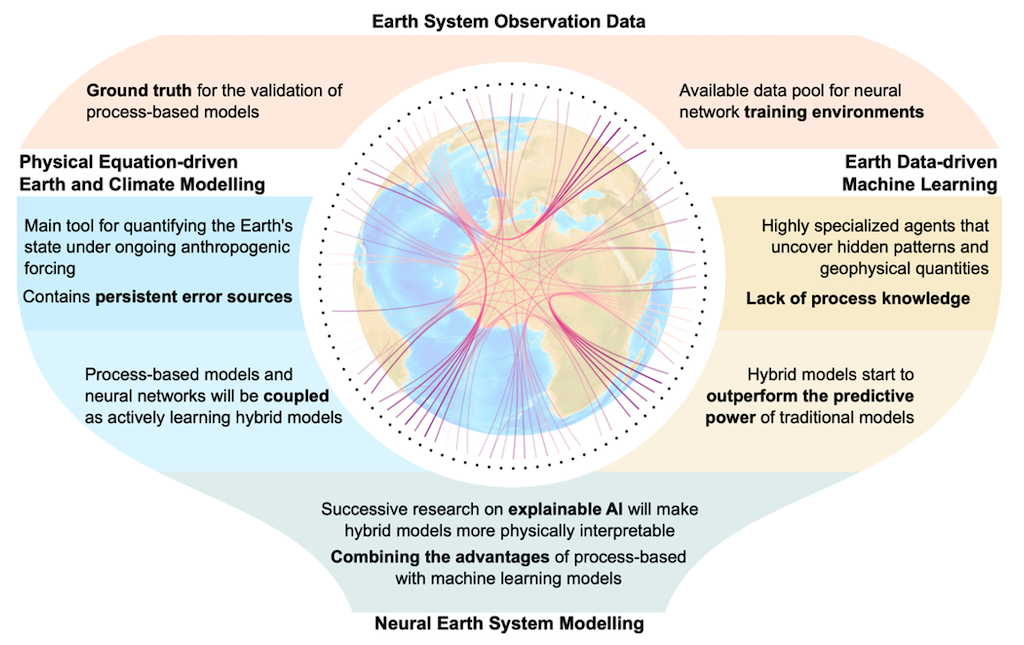
\includegraphics{fig/Neural_ESM.png}

\emph{Figure: Illustration of the stages of bringing ESMs and machine learning together towards neural Earth system modelling. The left and right branches visualise the current efforts and goals for building weakly coupled hybrids (blue and yellow), which converge towards strongly coupled hybrids. }

Within machine learning, making a correct prediction for the wrong reasons can be termed taking a ``shortcut'', or having a system description that is ``underdetermined''. Taking shortcuts is increasingly likely within climate science because the data available to us from the observational record is short and biased towards recent decades.

\href{https://www.carbonbrief.org/guest-post-how-artificial-intelligence-is-fast-becoming-a-key-tool-for-climate-science}{CarbonBrief Review}

\hypertarget{goal-index}{%
\section{Goal Index}\label{goal-index}}

In economic modelling choice of goal index (utility) function matters.
Daniel 2018\footnote{See Links to references} presents this figure:

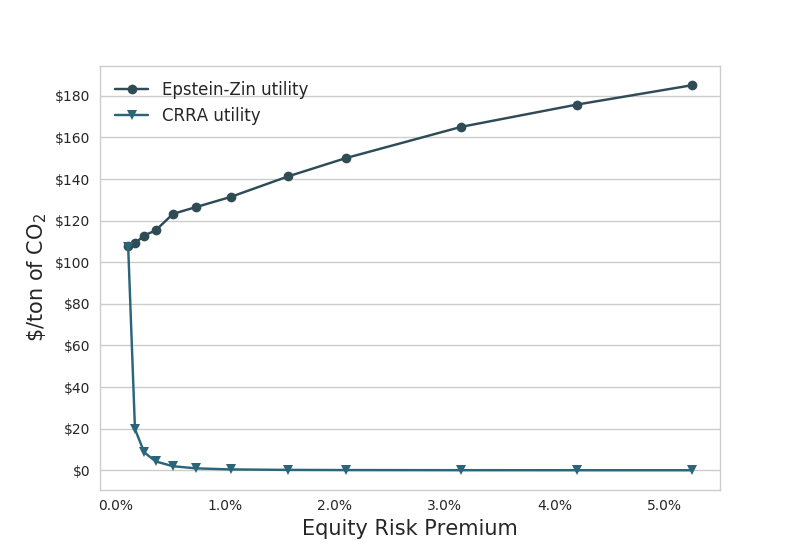
\includegraphics{fig/fig_EZvsCRRA_daniel2018fig1.png}

Fig. Optimal CO2-prices with increasing risk aversion for EZ vs CRRA utility specification. (From Daniel 2018)

As one of the co-authors explain: `We where not able to get the Social
Cost of Carbon (SCC) under \$120'.
That is for `reasonable risk aversion', using EZ-utilities.
The `standard' specification - with CRRA - utilities ends up with SCC
of \$20 or below.

\[V_1 = A [\tilde{C\_t}, \mu_t(V\_{t+1})]\]

Specification of the Goal Index function may seem a trivial technical issue -
no so!
There exists a broad professional litterature and profound discussions on
this matter -
which might de difficult to dis-entangle.

Let us begin with Frank Ramsey's growth model from 1928, commonly known
as the Ramsey-Cass-Koopmans model.

\(F(K,L)\) is an aggregate production function with factors \(K\) (Capital) and
\(L\) (Labour).

\hypertarget{model-drift}{%
\section{Model Drift}\label{model-drift}}

\emph{Abstract Sausen}

A method is proposed for removing the
drift of coupled atmosphere-ocean models, which
in the past has often hindered the application of
coupled models in climate response and sensitivity experiments.
The ocean-atmosphere flux fields
exhibit inconsistencies when evaluated separately
for the individual sub-systems in independent,
uncoupled mode equilibrium climate computations.
In order to balance these inconsistencies a
constant ocean-atmosphere flux correction field is
introduced in the boundary conditions coupling
the two sub-systems together. The method ensures
that the coupled model operates at the reference
climate state for which the individual model subsystems
were designed without affecting the dynamical response of the coupled system in climate
variability experiments. The method is illustrated
for a simple two component box model and an
ocean general circulation model coupled to a two
layer diagnostic atmospheric model.

\emph{Memo Barthel}

The coupling of different climate sub-systems poses a number of technical
problems. An obvious problem arising from the
different time scales is the synchronization or
matching of the numerical integration of subsys-
tems characterized by widely differing time steps.
A more subtle problem is

\emph{Model Drift}
When two general circulation models of the
atmosphere and ocean are coupled together in a
single model, it is generally found that the cou-
pled system gradually drifts into a new climate
equilibrium state which is far removed from the
observed climate. The coupled model climate
equilibrium may be so unrealistic (for example,
with respect to sea ice extent, or the oceanic equa-
torial current system) that climate response or
sensitivity experiments relative to this state be-
come meaningless. This occurs regularly even
when the individual models have been carefully
tested in detailed numerical experiments in the
decoupled mode and have been shown to yield
satisfactory simulations of the climate of the sepa-
rate ocean or atmosphere sub-systems.
The drift of the coupled model is clearly a sign
that something is amiss with the models. Howev-
er, we suggest that it is not necessary to wait with
climate response and sensitivity experiments with
coupled models unit all causes of model drift
have been properly identified and removed.
Model drift is, in fact, an extremely sensitive indi-
cator of model imperfections. The fact that the
equilibrium climate into which a coupled model
drifts is unacceptably far removed from the real
climate does not necessarily imply that the model
dynamics are too unrealistic for the model to be
applied for climate response and sensitivity ex-
periments. One should therefore devise methods
for separating the drift problem from the basically
independent problem of determining the change
of the simulated climate induced by a change in
boundary conditions a n d / o r external forcing (cli-
mate response), and from the question of the ef-
fect of changes in the physical or numerical for-
mulation of the model (model sensitivity).

\emph{Flux Correction}
The separation of the mean climate
simulation from the climate response or sensitiv-
ity problem can be achieved for coupled models
rather simply by an alternative technique, the flux
correction method.
The errors that result in a drift of the coupled
model are compensated in this method by con-
stant correction terms in the flux expressions by
which the separate sub-system models are cou-
pled together. The correction terms have no in-
fluence on the dynamics of the system in climate
response or sensitivity experiments, but ensure
that the ``working point'' of the model lies close to
the climate state for which the individual models
were originally tuned.
The basic principle of the flux correction method
is to couple the atmosphere and the ocean in such
a manner that in the unperturbed case each sub-
system simulates its own mean climate in the
same manner as in the uncoupled mode, but re-
sponds fully interactively to the other sub-system
in climate response or sensitivity experiments.

\href{pdf/Barthel_1988_Coupled_ocean_atmosphere_models_with_flux_corection.pdf}{Sausen (1988) Coupled Ocean-Atmosphere Model Drift Flux Correction (pdf)}

\hypertarget{model-evaluation}{%
\section{Model-evaluation}\label{model-evaluation}}

\emph{GCMeval: a tool for climate model ensemble evaluation}

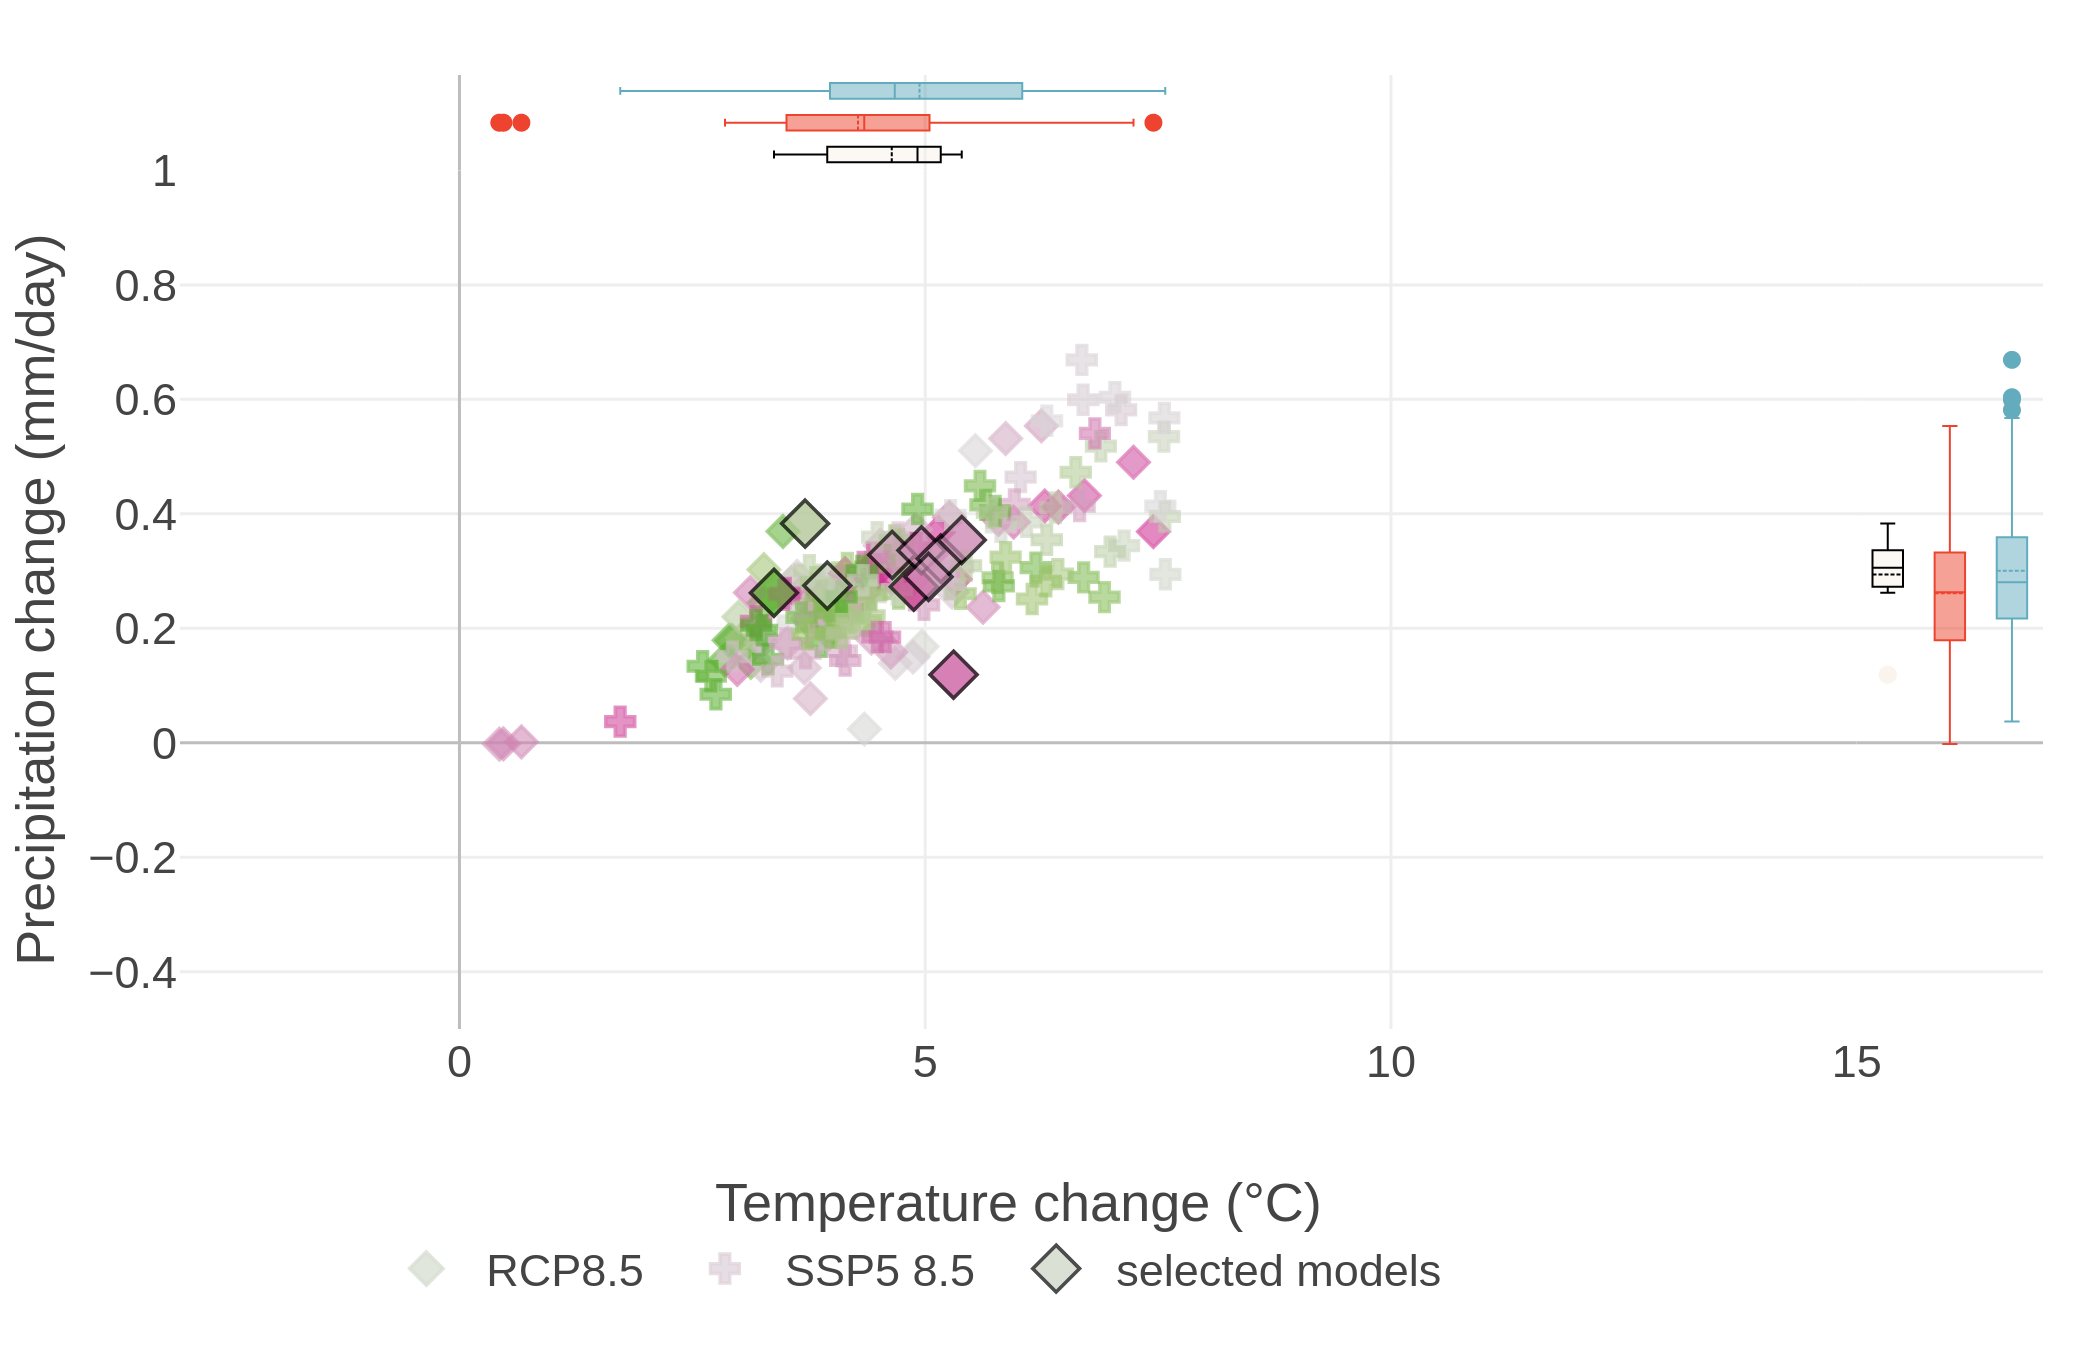
\includegraphics{fig/GCMevalNorthEuropeBestModels.png}

The global climate models indicate quite a range of future outcomes in terms of
precipitation and temperature.
To account for that, regional scenarios need to use fairly large multi-model ensembles.

\href{https://gcmeval.met.no/}{GCM-eval}

\hypertarget{measuering-forcings}{%
\subsection{Measuering Forcings}\label{measuering-forcings}}

Earth is on a budget -- an energy budget. Our planet is constantly trying to balance the flow of energy in and out of Earth's system. But human activities are throwing that off balance, causing our planet to warm in response.

Adding more components that absorb radiation -- like greenhouse gases -- or removing those that reflect it -- like aerosols -- throws off Earth's energy balance, and causes more energy to be absorbed by Earth instead of escaping into space. This is called a radiative forcing, and it's the dominant way human activities are affecting the climate.

limate modelling predicts that human activities are causing the release of greenhouse gases and aerosols that are affecting Earth's energy budget. Now, a NASA study has confirmed these predictions with direct observations for the first time: radiative forcings are increasing due to human actions, affecting the planet's energy balance and ultimately causing climate change.
The \href{https://agupubs.onlinelibrary.wiley.com/doi/10.1029/2020GL091585}{paper} was published online March 25, 2021, in the journal Geophysical Research Letters.

NASA's Clouds and the Earth's Radiant Energy System (CERES) project studies the flow of radiation at the top of Earth's atmosphere. A series of CERES instruments have continuously flown on satellites since 1997. Each measures how much energy enters Earth's system and how much leaves, giving the overall net change in radiation. That data, in combination with other data sources such as ocean heat measurements, shows that there's an energy imbalance on our planet.
But it doesn't tell us what factors are causing changes in the energy balance.

This study used a new technique to parse out how much of the total energy change is caused by humans. The researchers calculated how much of the imbalance was caused by fluctuations in factors that are often naturally occurring, such as water vapor, clouds, temperature and surface albedo (essentially the brightness or reflectivity of Earth's surface).
The researchers calculated the energy change caused by each of these natural factors, then subtracted the values from the total. The portion leftover is the radiative forcing.

The team found that human activities have caused the radiative forcing on Earth to increase by about 0.5 Watts per square meter from 2003 to 2018. The increase is mostly from greenhouse gases emissions from things like power generation, transport and industrial manufacturing. Reduced reflective aerosols are also contributing to the imbalance.

\href{https://www.nasa.gov/feature/goddard/2021/direct-observations-confirm-that-humans-are-throwing-earth-s-energy-budget-off-balance}{NASA Goddard Direct Observations of Forcings}

\hypertarget{values-in-climate-science}{%
\chapter{Values in Climate Science}\label{values-in-climate-science}}

\emph{Pulkkinen}

Values play a role in the construction of climate change information.

Science has its own values, including openness, objectivity and evidence-based thinking. However social values --- fundamental views on what is good, right and important --- guide a number of decisions in the construction, assessment and communication of information.

This marks a departure from the traditional `value-free ideal' of science, according to which social values should have a limited role in scientific research, while values that are epistemic (for example, precision and accuracy) are seen as legitimately influencing research.

Developing an acute awareness of how methodological choices and broader aims advantage different interests forms the first step in effectively managing the influence of values.

There is no neutral way of framing information.

Scientific research cannot be value-free, and climate science is no exception.

\textbf{The value of values in climate science}

To date, values are not widely acknowledged or discussed within physical climate science. Yet, effective management of values in physical climate science is required for the benefit of both science and society.

\textbf{Values in multimodel-based assessments}

A great number of research questions in climate science are answered by combining results from global climate model simulations within a multimodel framework and/or by their integration with observations. Winsberg20 argues that an opaque, inscrutable tapestry of values lies behind such results, due to the models' size and complexity, distributed epistemic agency and generative entrenchment of methodological choices. Any multimodel-based assessment must moreover deal with the questions of which models to include, and how to combine them. The extremes range from including all available models, for example, in a Coupled Model
Intercomparison Project context, and applying a one-model-one-vote principle, to selecting a single or very few flagship models. The underlying question of what is a good (enough) model is made explicit in model selection and implicit in model weighting, and relies on value-laden choices of metrics that may favour one spatial scale or region over another, one process over another or one stakeholder interest over another. This applies also to the AR6 approach of using a constrained ensemble of emulators for future projections, where the constraints are chosen to be based on simulation of past warming, equilibrium climate sensitivity and transient climate response.

\textbf{Values in event attribution}

Event attribution in its broadest sense is the evaluation of the contribution of causal factors to observed events. Two different methodological approaches to event attribution in climate science have been at times fiercely debated: the so-called probabilistic approach and the storylines approach, which occupy different positions on a spectrum of what level of conditioning on the meteorological circumstances is appropriate. A focus of debate has been the treatment of uncertainty in the dynamic response to anthropogenic forcing, given that uncertainty in the thermodynamic response is generally
much lower. It has been argued that the two sides fundamentally disagree about risk preferences. The proponents of the storylines approach are more concerned with false negatives (that is, falsely rejecting or underestimating anthropogenic influence on an event), and their methodology is supposedly less prone to this type of error, while it is the opposite for the probabilistic approach and its proponents. Both risk preferences, and hence preference for either methodology, are argued by Winsberg et al.~to be motivated by values, in particular by the balance between valuing epistemic confidence and informativeness.

\textbf{Values in climate services}

Climate services provide climate information to assist decision-making, aiming to support adaptation, mitigation and risk management decisions. This can be influenced by the values of all parties involved. Maximizing the fit of the information provided to the needs of the service users includes, in particular, the consideration of the users' value system. Parker and Lusk argue that a significant and feasible component is to match the risk preferences of the analysis to those of the users. This can be done by learning which types of errors the users find particularly undesirable;
recognizing methodological choices that differ in the risk of these errors; and making those choices in consultation with the users. For on-demand climate services, the authors suggest the use of clear warnings about product limitations and uncertainties in anticipation of various risk preferences, which allow for user customization at the point of service. Otherwise, they propose the prioritization of those user groups that might suffer especially severe harms and have limited access to climate information, and call for clear communication of which choices are influenced by values and how.

\href{https://www.nature.com/articles/s41558-021-01238-9.epdf?sharing_token=9sTaZge6-YVe29-rqhAuSdRgN0jAjWel9jnR3ZoTv0MW3oJvK3EImaMOhYg7TVKCUXr-xeCVyJ-lnFq2VH0GssNQt3AoQqZNQ5E7rSfw455t4_ZH4hJb0dBw9N22Lmlthe2YWgCjryCcYhhd_v-P1KPND7gwYWDiLyksdRInlw4\%3D}{Pulkinen (2022) The value of values in climate science (pdf sharedit)}

\hypertarget{part-climate-system}{%
\part{Climate System}\label{part-climate-system}}

\hypertarget{climate-system}{%
\chapter{Climate System}\label{climate-system}}

\hypertarget{convection}{%
\section{Convection}\label{convection}}

\emph{Zhang}

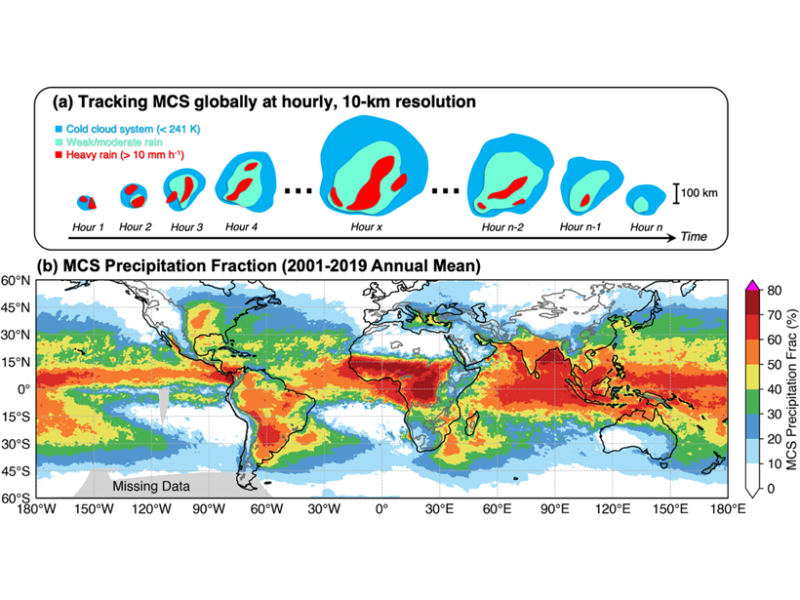
\includegraphics{fig/mesoscale_convection.png}

\emph{Figure: For the first time mesoscale convective systems (MCSs) in both the tropics and midlatitudes and all seasons can be tracked over many years by a new algorithm jointly using satellite observed cloud-top temperature and surface precipitation features at hourly and 10-km resolution globally (top panel). Results show that MCSs account for over 50\% of the annual rainfall across the tropics and many regions of the subtropics and midlatitudes (bottom panel).}

Mesoscale convective systems (MCSs) are a key component in the Earth's energy and hydrological cycles. They can grow to hundreds of kilometers in size, last for more than a day, and produce a majority of the annual rainfall in many regions of the world.

Past efforts to develop MCS databases have been limited to the tropics and used methodologies not well tested in the midlatitudes. Feng et al.~{[}2021{]} developed a new methodology to track MCSs globally using high-resolution satellite observations of both cloud and precipitation. The new method significantly improves the detection of MCSs in the midlatitudes. This new storm tracking database is the first to cover both the tropics and midlatitudes for all seasons.

The study shows that MCSs account for over 50 per cent of the annual rainfall across the tropics and many regions of the subtropics and midlatitudes. Storms over land have more intense convection, while those over oceans produce heavier rainfall and last longer.

This global MCS database supports a broad range of research such as understanding the role of MCSs in global extreme rainfall and circulation, and evaluation of global weather and climate model simulations.

\href{https://eos.org/editor-highlights/new-global-mesoscale-convective-system-tracking-database}{Zhang}

Convective storms of mesoscale dimension are a key component
in the Earth's energy and hydrological cycle. Mesoscale storms grow to hundreds of kilometers in size
and can last for more than a day, and produce a majority of the annual rainfall in many regions of the
world. Past studies of mesoscale storms have been limited to the tropics and used methodologies not well
tested in the midlatitudes. Here, we develop a new methodology to track mesoscale storms globally using
high-resolution satellite observations of both cloud and precipitation. The satellite-based storm tracking
reproduces important storm statistics derived from ground-based radar observations. Our new method
significantly improves the detection of mesoscale storms in the midlatitudes. This new storm tracking
database is the first to cover both the tropics and midlatitudes for all seasons. Results show that mesoscale
convective storms account for over 50\% of annual rainfall across the tropics and many regions of the
subtropics and midlatitudes. Storms over land have more intense convection, while those over ocean
produce heavier rainfall and last longer. This global mesoscale storms tracking database supports a broad
range of applications, such as understanding their role in global extreme rainfall and circulation and
evaluation of global weather and climate model simulations.

\href{https://agupubs.onlinelibrary.wiley.com/doi/10.1029/2020JD034202}{Feng (2021) Mesoscale Convective System}
\href{pdf/Feng_2021_Mesoscale_Convective_System.pdf}{(pdf)}

\hypertarget{earth-energy-imbalance-eei}{%
\section{Earth Energy Imbalance (EEI)}\label{earth-energy-imbalance-eei}}

\emph{Loeb Abstarct}

Earth's Energy Imbalance (EEI) is a relatively small (presently ∼0.3\%) difference between global mean solar radiation absorbed and thermal infrared radiation emitted to space. EEI is set by natural and anthropogenic climate forcings and the climate system's response to those forcings. It is also influenced by internal variations within the climate system. Most of EEI warms the ocean; the remainder heats the land, melts ice, and warms the atmosphere. We show that independent satellite and in situ observations each yield statistically indistinguishable decadal increases in EEI from mid-2005 to mid-2019 of 0.50±0.47 W m-2 decade-1 (5\%-95\% confidence interval). This trend is primarily due to an increase in absorbed solar radiation associated with decreased reflection by clouds and sea-ice and a decrease in outgoing longwave radiation (OLR) due to increases in trace gases and water vapor. These changes combined exceed a positive trend in OLR due to increasing global mean temperatures.

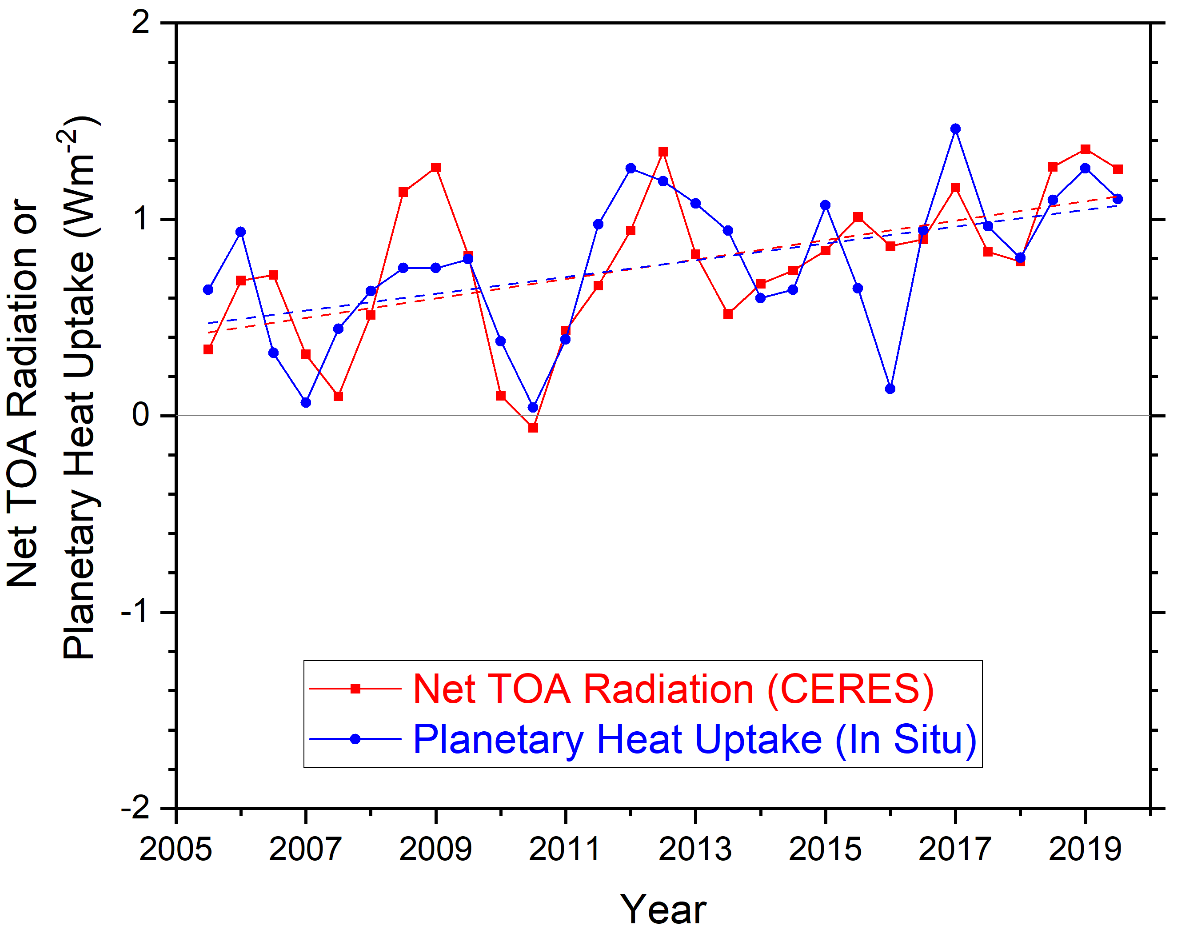
\includegraphics{fig/earth_energy_imbalance.png}

\emph{Figure: Comparison of overlapping one-year estimates at 6-month intervals of net top-of-the-atmosphere annual
energy flux from the CERES EBAF Ed4.1 product (solid red line) and an in situ observational estimate of uptake of
energy by Earth climate system (solid blue line). Dashed lines correspond to least squares linear regression fits to the data}

\href{https://agupubs.onlinelibrary.wiley.com/doi/10.1029/2021GL093047}{Loeb (2021) Satellite and Ocean Data Reveal Marked Increase in Earth's Heating Rate}
\href{pdf/Loeb_2021_Earths_Heating_Rate.pdf}{(pdf)}
\href{https://www.nasa.gov/feature/langley/joint-nasa-noaa-study-finds-earths-energy-imbalance-has-doubled}{NASA}
\href{https://www.theguardian.com/science/2021/jun/17/earth-trapping-heat-study-nasa-noaa}{Guardian}

\hypertarget{energy-imbalance-trend-teei}{%
\subsection{Energy Imbalance Trend (TEEI)}\label{energy-imbalance-trend-teei}}

\emph{Raghuraman Abstract}

The observed trend in Earth's energy imbalance (TEEI), a measure of the acceleration of heat uptake by the planet, is a fundamental indicator of perturbations to climate. Satellite observations (2001--2020) reveal a significant positive globally-averaged TEEI of 0.38 ± 0.24 \(Wm^{-2} decade^-1\), but the contributing drivers have yet to be understood. Using climate model simulations, we show that it is exceptionally unlikely (\textless1\% probability) that this trend can be explained by internal variability. Instead, TEEI is achieved only upon accounting for the increase in anthropogenic radiative forcing and the associated climate response. TEEI is driven by a large decrease in reflected solar radiation and a small increase in emitted infrared radiation. This is because recent changes in forcing and feedbacks are additive in the solar spectrum, while being nearly offset by each other in the infrared. We conclude that the satellite record provides clear evidence of a human-influenced climate system.

\emph{Raghuraman Memo}

Earth's energy imbalance (EEI) is the difference between the
incoming solar radiation (S 0 ), and the reflected shortwave
radiation (RSW) plus the outgoing longwave radiation
(OLR), at the top of the atmosphere. Thus, EEI is a fundamental
measure of the degree to which the Earth's global climate
system is out of balance. A trend in EEI measures the acceleration
of heat uptake by the planet and hence is an indicator of perturbations
to the coupled atmosphere-ocean-land-ice system.
The mean EEI during 2005--2015 was estimated to be
0.71 ± 0.10 \(Wm^{-2}\) . Oceans store 90\% of this excess heat. Because
of this close relationship between EEI and ocean heating, EEI
trends have an important bearing on the warming of the global
climate system, sea-level rise, and marine health.

In the contemporary climate system, internal variability (ε),
effective radiative forcing (ΔERF), and the radiative response
(λΔT s ) change EEI. Thus, an anomaly in EEI can be
expressed as the sum of these three terms.

\[ΔEEI = ΔERF + λΔT_s+ ε\]

Climate feedbacks and surface temperature are represented by
λ and \(T_s\) respectively.

While we know
that TEEI is influenced by internal variability in the climate
system, external forcings, and climate feedbacks, the extent of the
contribution from each has not been previously determined.

In particular, due to the inherent noise in the Earth system, a
single observed 20-year time series of EEI is only one of many
possible time series that internal variability could produce,
and therefore, it is imperative to quantify the contribution of
internal variability (ε) to TEEI.

We focus here on the investigation of the trend in EEI (TEEI).
In particular, the contributions to TEEI by the drivers of the OLR
and RSW trends, are an unexplored and unquantified area in the
explanation of the observed satellite record.

We use Coupled
Model Intercomparison Project Phase 6 (CMIP6) experiments
and design a hierarchy of climate model experiments with the
Geophysical Fluid Dynamics Laboratory Coupled/Atmospheric
Model 4.0 (GFDL CM4/AM4)to better understand the
contributions of the three components of Eq. (1) to the CERES-
observed TEEI, thereby providing an assessment of the relative
importance of anthropogenically induced changes versus internal
variability changes. We show that anthropogenic forcing and the
associated climate response yield the observed positive TEEI.

The observed ΔEEI time series
yields a significant positive trend of 0.38 ± 0.24 \(Wm^-2 decade^-1\)
There is, however, the potential for systematic
errors associated with the observed trend due to instrument drift.
The trend is driven by large reductions in RSW,
compensated only by a relatively weaker increase in OLR.

The observed trend in EEI is unexplained by internal varia-
bility. Our hierarchy of modeling experiments allows us to
investigate the possible contributions of trends in ΔERF, \(λΔT_s\) ,
and ε to TEEI. We compose five sets of estimates of the internal
variability (ε) using climate model simulations. For all five sets of
estimates, we calculate ε as the ±2σ range of 20-year trends across
the realizations.

We find that the CERES-observed TEEI lies outside the range
of trends driven by internal variability alone.

ε comprises a range of trends in EEI due to internal
variability, the value of ε, ±0.19 \(Wm^{-2} decade^−1\)

The satellite-observed positive EEI trend over the 2001--2020
period is exceptionally unlikely (\textless1\% probability) to be
explained by internal variability.

\href{https://www.nature.com/articles/s41467-021-24544-4}{Raghuraman (2021) Anthropogenic forcing and response yield observed positive trend in Earth's energy imbalance}
\href{pdf/Raghuraman_2021_TEEI.pdf}{(pdf)}

\emph{NBCnews}

Stability in Earth's climate hinges on a delicate balance between the amount of energy the planet absorbs from the sun and the amount of energy Earth emits back into space. But that equilibrium has been thrown off in recent years --- and the imbalance is growing, according to a paper published Wednesday in the journal Nature Communications.

The Princeton University researchers behind the paper found that there's a less than 1 percent probability that the changes occurred naturally.

The findings undercut a key argument used by people who do not believe human activity is responsible for the bulk of climate change to explain trends in global warming, demonstrating that the planet's energy imbalance cannot be explained just by Earth's own natural variations.

\href{https://www.nbcnews.com/science/environment/earths-energy-imbalance-removes-almost-doubt-human-made-climate-change-rcna1562}{nbcnews}

\hypertarget{jet-stream}{%
\section{Jet Stream}\label{jet-stream}}

\emph{Rousi}

\textbf{Accelerated western European heatwave trends linked to more-persistent double jets over Eurasia}

Persistent heat extremes can have severe impacts on ecosystems and societies, including excess mortality, wildfires, and harvest failures. Here we identify Europe as a heatwave hotspot, exhibiting upward trends that are three-to-four times faster compared to the rest of the northern midlatitudes over the past 42 years. This accelerated trend is linked to atmospheric dynamical changes via an increase in the frequency and persistence of double jet stream states over Eurasia. We find that double jet occurrences are particularly important for western European heatwaves, explaining up to 35\% of temperature variability. The upward trend in the persistence of double jet events explains almost all of the accelerated heatwave trend in western Europe, and about 30\% of it over the extended European region. Those findings provide evidence that in addition to thermodynamical drivers, atmospheric dynamical changes have contributed to the increased rate of European heatwaves, with implications for risk management and potential adaptation strategies.

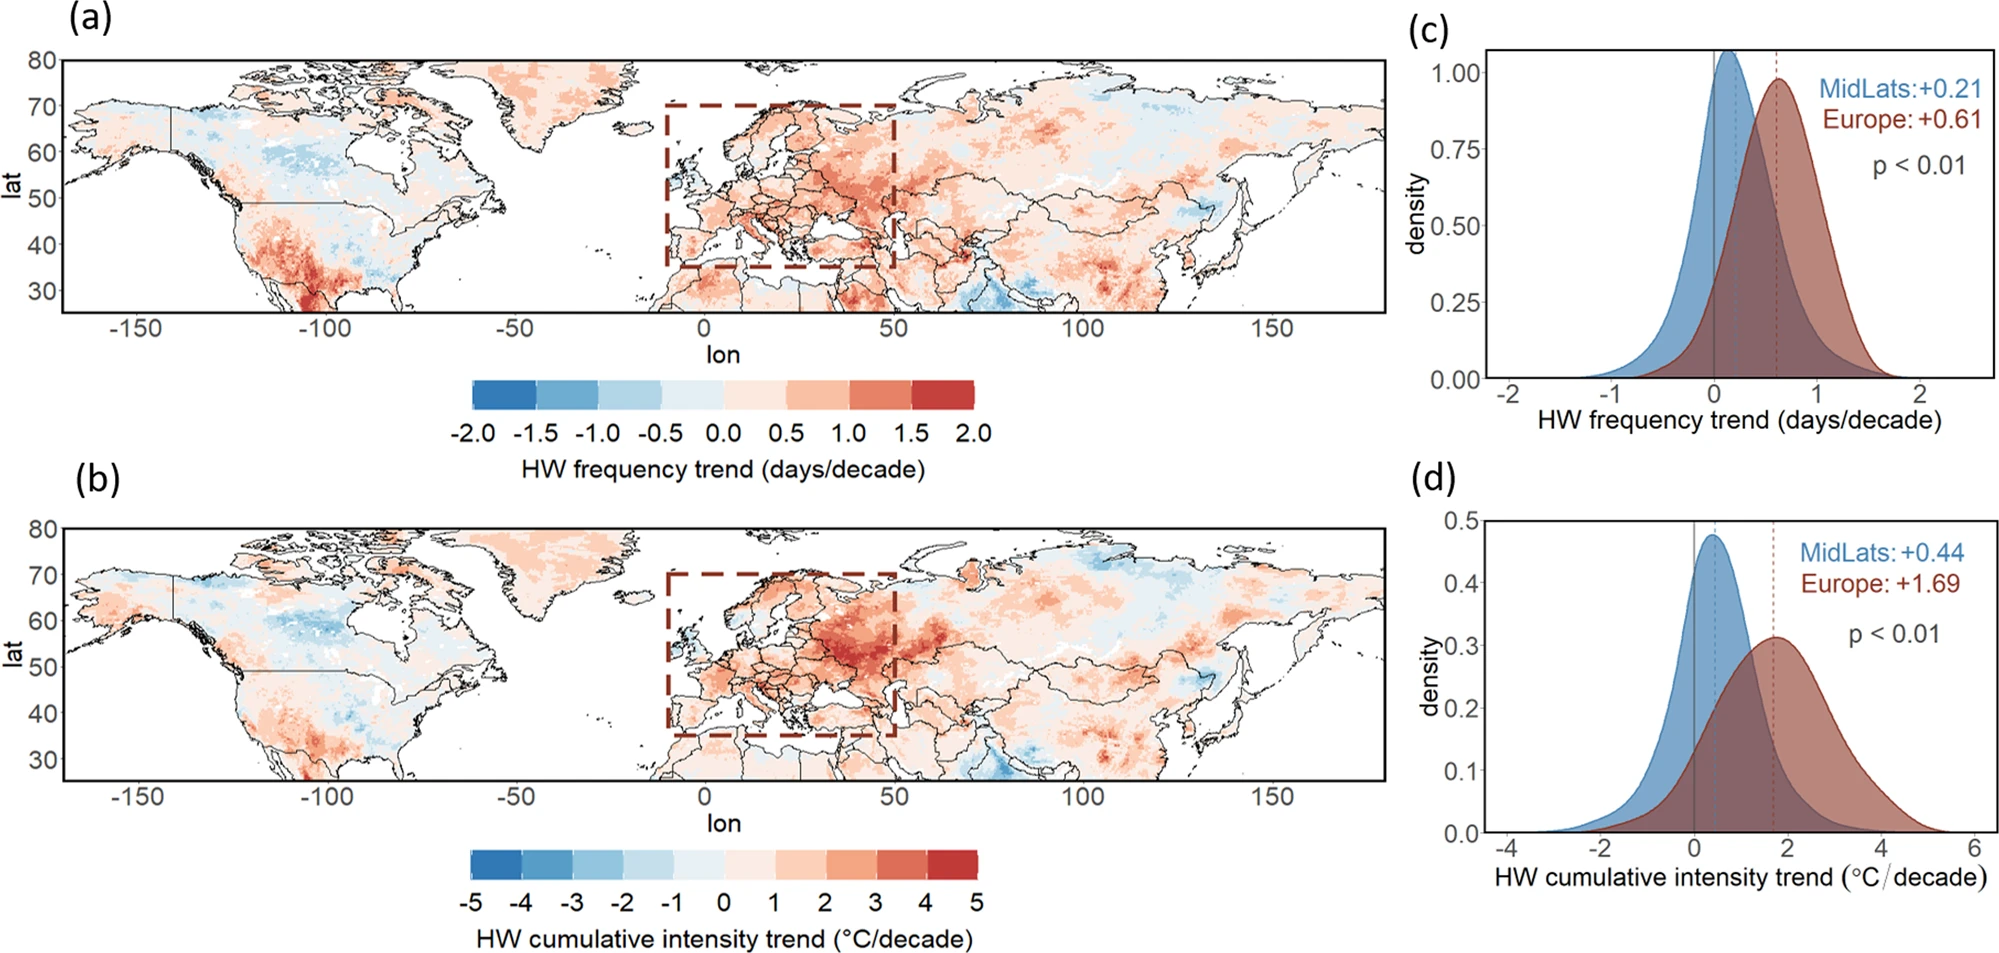
\includegraphics{fig/heatwave_europe.png}

\href{https://www.nature.com/articles/s41467-022-31432-y}{Rousi (2022) Accelerated western European heatwave trends linked to more-persistent double jets over Eurasia}

\hypertarget{total-solar-irradiance}{%
\section{Total Solar Irradiance}\label{total-solar-irradiance}}

\emph{Climate.gov: Incoming Sunlight}

\textbf{the Sun likely added at most 0.01 degrees Celsius to the 0.95--1.2 degrees Celsius of global surface warming that's occurred since pre-industrial times.}

\begin{quote}
Satellite observations through several solar cycles reveal that the difference in total average brightness between solar maxima and minima is very small, on the order of 1 Watt per square meter during strong cycles. On average, the Sun delivers 1,361 Watts of power per square meter at a distance of one astronomical unit. This amount is known as the total solar irradiance. Based on observations and models, experts estimate that the impact of this 11-year variation on global surface temperature is likely around 0.1 degrees Celsius or less.
\end{quote}

\begin{itemize}
\tightlist
\item
  The Sun's overall brightness varies on timescales from minutes to millennia, and these changes are detectable in the global temperature record.
\item
  During strong solar cycles, the Sun's total average brightness varies by up to 1 Watt per square meter; this variation affects global average temperature by 0.1 degrees Celsius or less.
\item
  Changes in the Sun's overall brightness since the pre-industrial period have been minimal, likely contributing no more than 0.01 degrees Celsius to the roughly 1 degree of warming that's occurred over the Industrial period.
\item
  Projected warming due to increasing greenhouse gas levels in the coming decades will overpower even a very strong Grand Solar Minimum.
\item
  Rising amounts of atmospheric carbon dioxide have postponed the next Milankovitch-driven ice age by at least tens of thousands of years.
\end{itemize}

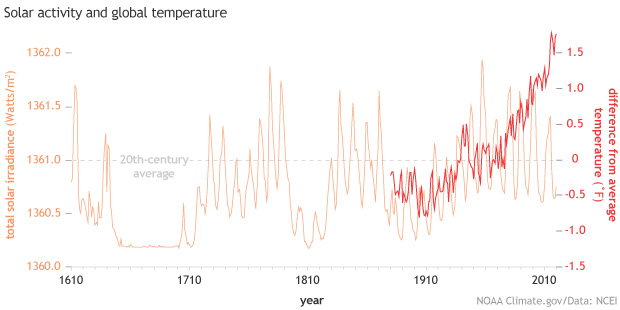
\includegraphics{fig/TSI_vs_globaltemp.jpg}

\emph{Figure: Yearly total solar irradiance (orange line) from 1610--2020 and the annual global temperature compared to the 20th-century average (red line) from 1880--2020. Since the middle of the 20th-century, solar activity has declined while global temperature increased rapidly. NOAA Climate.gov image, based on solar data from Coddington et al., 2016, and temperature data from NOAA NCEI.}

Even if the Sun's recent quietness---the 11-year cycle minimum in 2011 was the lowest in a century---were to turn into a multi-decade stretch of extremely low activity known as a Grand Solar Minimum, it wouldn't overpower the amount of global warming projected for the coming century due to increasing greenhouse gas emissions. In fact, as long as atmospheric carbon dioxide remains above 300 parts per million, not even the next ice age, which Milankovitch theory predicts would begin 50,000 years from now, is likely to occur.

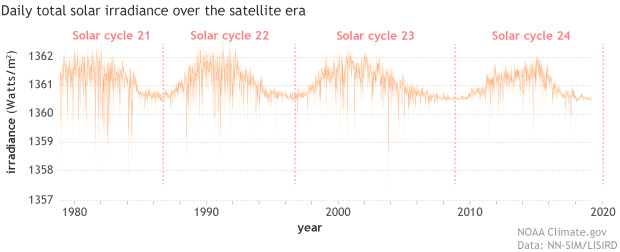
\includegraphics{fig/nn_sim_tsi_satelliteera.jpg}

\emph{Figure: Daily observations of total solar irradiance (orange line) since the start of the satellite era in 1978. Day-to-day, TSI may vary by as much as 0.3 percent, but average differences between maximum and minimum are on the order 0.1 percent, or around 1 Watt per square meter. NOAA Climate.gov image, based on data from LASP Interactive Solar Irradiance Data Center.}

Scientists today have close to four decades of overlapping measurements of total solar irradiance and sunspots, which allow them to statistically describe how changes in sunspot numbers relate to variations in total solar irradiance. They've used that relationship to model the Sun's brightness back to the start of the sunspot record in the 1600s.

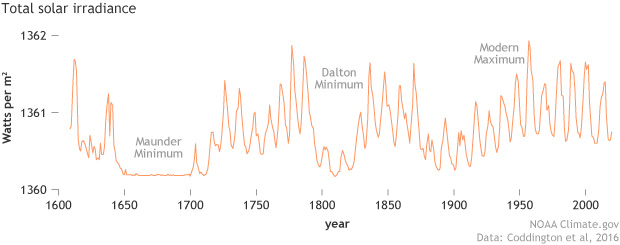
\includegraphics{fig/TSI_1610-2020.jpg}

\emph{Figure: Total solar irradiance estimated from sunspot observations since 1610. NOAA Climate.gov image, based on the NOAA TSI Climate Data Record (Coddington et al., 2016).}

These historical reconstructions reveal that some solar cycles are more active than others, and that their timing isn't completely random. Generally, 2-3 relatively strong cycles will be preceded and followed by 2-3 relatively weak ones. These alternating strong and weak epochs tend to be grouped together over approximately 100-year periods, a pattern known as Gleissberg cycles. Over the span of the historical sunspot record, there have been three \textasciitilde100-year Gleissberg cycles: 1700-1810, 1810-1910, and 1910-2010.

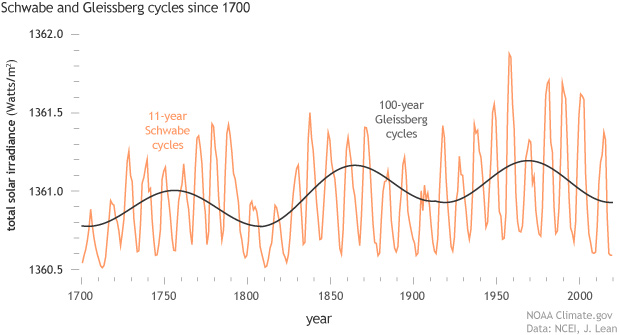
\includegraphics{fig/Schwabe_Gleissberg_1700-2020.jpg}

\emph{Figure: The amplitude of the 11-year solar cycle (formally called the Schwabe cycle, orange) is modulated by the approximately 100-year Gleissberg cycle (charcoal), in which a number of consecutive cycles of high activity are bracketed by consecutive cycles of lower activity. The start of the Industrial Revolution in the mid-1700s coincided with a Gleissberg maximum. The relatively high activity of the mid 20th-century also coincided with a Gleissberg maximum, while the recent decades coincide with a Gleissberg minimum. NOAA Climate.gov image based on data from Wang and Lean, 2021.}

In addition, the record shows that there have been periods when sunspots virtually disappear for several decades. (Other features of the 11-year solar cycle continue to occur, however.) These periods are called Grand Solar Minimums. For example, between 1645-1715, the Sun went through a 70-year quiet period known as the Maunder Minimum. Sunspots disappeared almost completely, and the solar wind was maybe half of its modern velocity. The Maunder Minimum partially overlapped a centuries-long cold spell called the Little Ice Age, which was strongest in the Northern Hemisphere between 1450­-1850.

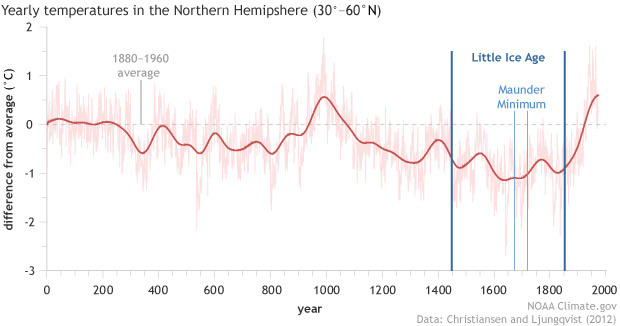
\includegraphics{fig/NH_temp_2000yrs.jpg}

\emph{Figure: A 2000-year temperature history of the Northern Hemisphere outside the tropics shows a warm period that peaked around 1,000 A.D. followed by a multi-century period of cooling: the Little Ice Age. The coldest part of the Little Ice Age overlapped the very low solar activity of the Maunder Minimum, but the cold spell began well before. NOAA Climate.gov graph, based on data from Christiansen and Ljungqvist, 2012.}

In contrast, the Sun was unusually active in the twentieth century, a period which solar experts call the Modern Maximum. Starting near the turn of the twentieth century, each solar cycle was increasingly active. This build up was tied to the last Gleissberg Cycle, which peaked during solar cycle 19 in 1957. Solar activity then declined in the second half of the 20th-century. The stretch of high activity drew to a definite close in the first decade of the twenty-first century with solar cycle 23, which had an unusually long and low minimum. Solar cycle 24 went on to have one of the lowest maximums of the last 70 years, and solar cycle 25 is expected to be comparable. Meanwhile, Earth's surface temperatures continued to rise rapidly.

The increasing solar activity of the first half of the 20th century and the decreasing activity since then have largely canceled each other out in terms of their influence on global temperature.

The modern sunspot record tells us about solar activity over the past four centuries. Indirect evidence for solar activity deeper in the past comes from the presence of cosmogenic isotopes---radioactive atoms that are generated when common isotopes of an element are struck by galactic cosmic rays.

Our solar system is constantly bombarded with galactic cosmic rays, but the Sun's magnetic field shields us from most of them. When the Sun's magnetic field is strong, at solar maximum, fewer cosmic rays reach the atmosphere, creating very few cosmogenic isotopes. At solar minimum, when the Sun's magnetic field is weaker, slightly more cosmic rays reach Earth's atmosphere, generating more cosmogenic isotopes. The two most common cosmogenic isotopes are carbon-14, which can be found in tree rings, and beryllium-10, which is found in ice cores. Using fluctuations in cosmogenic isotopes, experts have reconstructed solar activity back thousands of years.

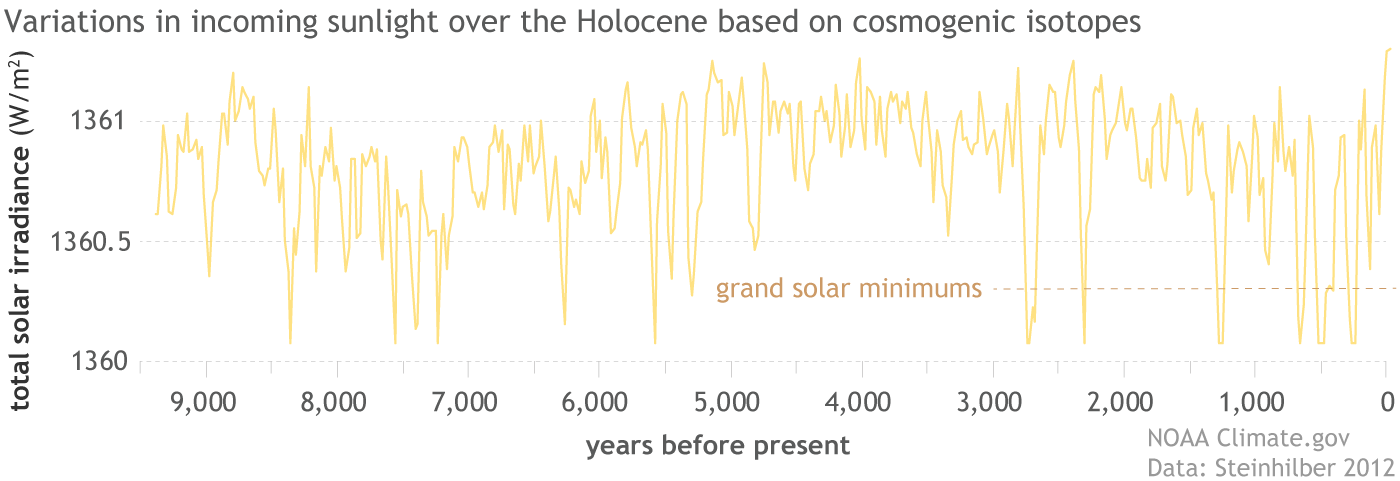
\includegraphics{fig/TSI_cosmogenic_holocene_1400.png}

\emph{Figure: A reconstruction of total solar irradiance over the past 9,400 years based on a combination of carbon-14 isotopes in tree rings and beryllium-10 in ice cores. The record indicates there have been at least 25 Grand Solar Minimums in the Holocene. NOAA Climate.gov image, based on data from Steinhilber et al., 2012.}

These paleoclimate reconstructions reveal that the Sun has produced at least 25 grand minimums in the past 9,000 years. Some are short---just two or three decades---and others, like the Maunder Minimum, are five or more decades. They occur every 200 years or so, a period known as the de Vries cycle. Many of them were preceded by a solar cycle with an unusually long and low solar minimum, similar to the minimum of 2008.

\textbf{Milankovitch cycles and ice ages}

The 11-year sunspot cycle and its Gleissberg-cycle modulation cause small changes in the Sun's actual brightness---how much sunlight the Sun radiates to Earth. Earth's climate is also affected by how much sunlight reaches us due to changes in our planet's orbit and position in space relative to the Sun. Called Milankovitch cycles, these predictable orbital patterns have repeat times of tens to hundreds of thousands of years.

For the past million years at least, Milankovitch cycles have coincided with 100,000-year-long ice ages punctuated by short intervals of rapid warming. Although there are pieces of the puzzle experts still don't understand, the key climate influence seems to be changes in the amount of incoming sunlight, or insolation, reaching the high latitudes of the Northern Hemisphere during the summer. The Northern Hemisphere is key to the ice ages because massive ice sheets can only grow over land, not ocean, and most of Earth's land area has been concentrated in the Northern Hemisphere for at least tens of millions of years.

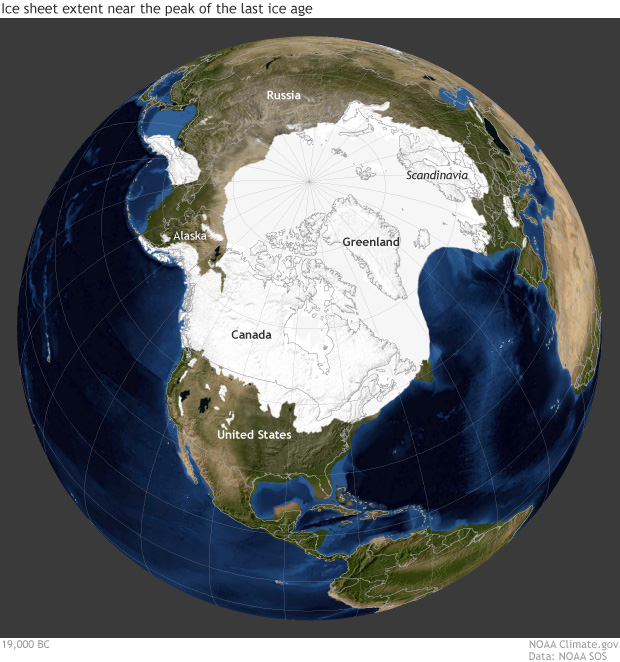
\includegraphics{fig/GlacialMax.jpg}

\emph{Figure: Changes in Northern Hemisphere sunlight are the key to ice ages because massive ice sheets, such as the one that spread across North America and Eurasia roughly 20,000 years ago, can only grow over land, and most land area has been in the Northern Hemisphere for tens of millions of years. (High-resolution without annotations available.) Image by Climate.gov based on data from Science on a Sphere.}

The most significant changes in Northern Hemisphere insolation come from three variations in Earth's orbit:

\begin{verbatim}
precession (~26,000 years): the slow rotation or “wobble” in the Earth’s axis of rotation, which changes where in the annual orbital path Northern Hemisphere summer solstice occurs;
obliquity (~41,000 years): how tilted Earth’s axis of rotation is;
eccentricity (~100,000 years): how far Earth’s orbit is from being a perfect circle.
\end{verbatim}

Because these cycles have different lengths, they overlap in complex rhythms, reinforcing one another at some times and offsetting one other at others. Northern Hemisphere summer insolation is maximized when tilt is extreme, eccentricity is extreme, and precession causes Northern Hemisphere summer solstice to occur near perihelion, the place in its orbit when Earth is closest to the Sun. Summer insolation is minimized when tilt is smaller, eccentricity is extreme, and Northern Hemisphere summer solstice occurs near aphelion, when Earth is farthest from the Sun.

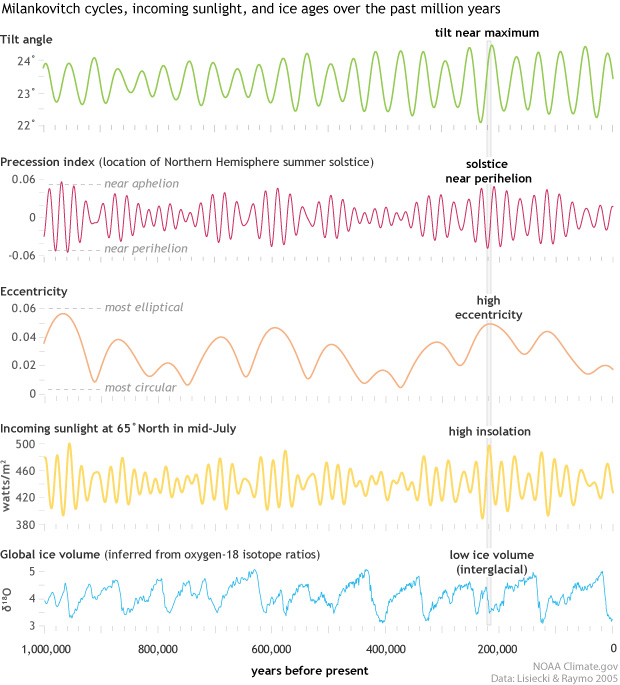
\includegraphics{fig/orbital_cycles_sunlight_ice.jpg}

\emph{Figure: Rows 1-3) Milankovitch cycles over the past million years (tilt, precession, and eccentricity. (Row 4) Northern Hemisphere summer insolation. (Row 5) Global ice volume inferred from oxygen isotopes in sea floor sediments. Light gray column highlights conditions around 220,000 years ago, when overlap among the three orbital cycles brought a peak in Northern Hemisphere insolation, triggering a warming period with low ice sheet volume. NOAA Climate.gov image, based on data from Lisiecki and Raymo, 2005.}

How low summer insolation must fall to trigger an ice age depends on how high atmospheric carbon dioxide levels are; the more carbon dioxide, the lower the insolation must be. Looking back over the past million years, the highest carbon dioxide level at the start of any ice age was 300 ppm, and most were far lower.

At pre-industrial carbon dioxide levels, summer insolation at 65° North need only dip 0.75 standard deviations below the mean---about 15 Watts per square meter---for summers to be too cool to melt all the winter snow, a low that Milankovitch cycles predict we will next hit about 50,000 years from now. At 400 parts per million, summer insolation would need to fall twice as much---a low we will next see 125,000 years from now. At carbon dioxide levels above 560 parts per million no Milankovitch variation within the next half million years will be low enough to trigger an ice age.

\href{https://www.climate.gov/news-features/understanding-climate/climate-change-incoming-sunlight}{Climate.gov: Incoming Sunlight}

\emph{Danish ISAC Study}

Conclusions

The Sun
- Sunspot number catches only part of solar activity
- The Sun's magnetic field drives short term changes
- Use therefore magnetic data for Sun-Climate studies
- Solar output predictability is at most years ahead
- Due to the complexity and time-varying nature of the Sun solar-climate coupling must be expected to be very complex and probably changing with time

The total solar irradiance (TSI) is in a sense the most obvious solar parameter to single
out for study when considering the Sun-climate connection. The power input received by
the Earth from the Sun is the driver of Earth's climate system and the variations in TSI do
correlate reasonably well with the variations seen in the climate. However, the brute
variations in power received at Earth are not strong enough to explain the variations in
climate that are observed.
For TSI to be the driver of the climate variations observed some
sort of amplification or feedback mechanism must therefore be in place.

The influence of TSI on the climate is multifaceted. Variations in TSI translate to
different heating in various layers of the atmosphere (though UV here plays the major
role), heat absorption in the oceans with different time scales from those of the
atmosphere, differential heating over land and oceans, etc. These primary influences from
TSI will in turn alter such things as atmospheric circulation, water vapour content in the
atmosphere, and cloud cover. Effects from these secondary phenomena may then feed
back into the energy absorbed by the climate system from solar irradiation, for example
via changes in the Albedo, possibly enhancing the effects of TSI variations.
Due to the geographically heterogeneous nature of solar influence on climate and the
rather complicated feedback mechanisms involved in solar forcing of the climate any
simple explanation of TSI-climate connections is likely to fail, except in limited cases
such as variations in sea surface temperature that seem to be at least partly explainable by
simple energy balance considerations.

\href{pdf/ISAC_2007_Solar.pdf}{Danish national Space Center (2007) Influence of Solar Activity Cucles on Earth's Climate (pdf)}
\href{pdf/ISAC_2007_Solar_Presentation.pdf}{Presentation (pdf)}

\hypertarget{spatial-shock}{%
\section{Spatial Shock}\label{spatial-shock}}

\hypertarget{coastal-flooding}{%
\subsection{Coastal Flooding}\label{coastal-flooding}}

\emph{Desmet}

\textbf{Just moving to higher grounds}

Nobel Prize winner William Nordhaus has called climate change ``the ultimate challenge for economics.''

Economists increasingly have been trying to understand how rising tides and global temperatures will impact resource allocation around the globe, as well as the potential policy tools that can help curb damage to our natural world.

SMU professor Klaus Desmet says that a lot of those analyses are missing a critical factor: migration.

Desmet coauthored a paper in the American Economic Journal\href{https://www.aeaweb.org/articles?id=10.1257/mac.20180366}{Evaluating the Economic Cost of Coastal Flooding (paywall)}: Macroeconomics that examines how economic output will be affected over the next 200 years as humans move away from coastal areas threatened by rising sea levels. Although losses in vulnerable Southeast Asian cities such as Bangkok and Shanghai will still be very significant, their research shows that overall GDP declines are substantially less than predicted by models that don't account for spatial shifts in economic activity.

\begin{quote}
Climate change is to a large extent a spatial shock.
\end{quote}

\begin{quote}
Migration as one of the key responses to climate change.
\end{quote}

What we find in our model is that at a global level, flooding decreases real GDP by about 0.1 percent by the year 2200. If we were to completely ignore the dynamic spatial response of the economy, if we were to have everyone stay put in the face of rising seas, then the loss would actually increase to 4.5 percent. So, that difference between 0.1 and 4.5 percent underscores the first-order importance of taking into account moving, migration, and the spatial dynamic response of the economy to rising sea levels.

We develop a high resolution dynamic model of the world economy. This model splits up the world into 64,800 1° by 1° grid cells, which are linked to each other through trade and migration. We feed into this model high-quality projections of both global and local sea level rise over the next 200 years. . . . When we run our model forward, we can then assess what the economic effect will be of having these pieces of land lost for production.

We find large losses in coastal areas of south and east Asia, with countries such as Vietnam, Thailand, and Bangladesh losing up to 10 percent of real GDP in present discounted value terms over the next 200 years. Other areas that will also suffer disproportionately include coastal Northwest Europe, {[}and{]} some areas on the US East Coast and Gulf Coast. By contrast, the Pacific Coast of the Americas is much less affected and, in fact, most of the coastal areas of Africa are also a lot less affected.

\href{https://www.aeaweb.org/research/klaus-desmet-migration-climate-change}{Desmet}

\hypertarget{climate-stability}{%
\chapter{Climate Stability}\label{climate-stability}}

\emph{Crona}

Climate stability is a service provided by a healthy biosphere,
through complex interconnections between land, water, and
atmosphere.

\href{https://www.sciencedirect.com/science\%20/article/pii/S2590332221002359\#undfig1}{Crona (2021) The Anthropocene reality of financial risk}
\href{pdf/Crona_2021_Anthropocene_reality_of\%20Financial_Risk.pdf}{(pdf)}
\href{pdf/Crona_2021_Anthropocene_reality_of\%20Financial_Risk_SI.pdf}{(pdf SI)}
\href{https://www.cell.com/one-earth/fulltext/S2590-3322(21)00235-9?_returnURL=\%20https\%3A\%2F\%2Flinkinghub.elsevier.com\%2Fretrieve\%2Fpii\%2FS2590332221002359\%3Fshowall\%3Dtrue}{Alt link: One Earth}

\hypertarget{tipping}{%
\chapter{Tipping}\label{tipping}}

\emph{Wunderling Abstract}

With progressing global warming, there is an increased risk that one or several tipping elements in the climate system might cross a critical threshold, resulting in severe consequences for the global climate, ecosystems and human societies. While the underlying processes are fairly well-understood, it is unclear how their interactions might impact the overall stability of the Earth's climate system. As of yet, this cannot be fully analysed with state-of-the-art Earth system models due to computational constraints as well as some missing and uncertain process representations of certain tipping elements. Here, we explicitly study the effects of known physical interactions among the Greenland and West Antarctic ice sheets, the Atlantic Meridional Overturning Circulation (AMOC) and the Amazon rainforest using a conceptual network approach. We analyse the risk of domino effects being triggered by each of the individual tipping elements under global warming in equilibrium experiments. In these experiments, we propagate the uncertainties in critical temperature thresholds, interaction strengths and interaction structure via large ensembles of simulations in a Monte Carlo approach. Overall, we find that the interactions tend to destabilise the network of tipping elements. Furthermore, our analysis reveals the qualitative role of each of the four tipping elements within the network, showing that the polar ice sheets on Greenland and West Antarctica are oftentimes the initiators of tipping cascades, while the AMOC acts as a mediator transmitting cascades. This indicates that the ice sheets, which are already at risk of transgressing their temperature thresholds within the Paris range of 1.5 to 2 ∘C, are of particular importance for the stability of the climate system as a whole.

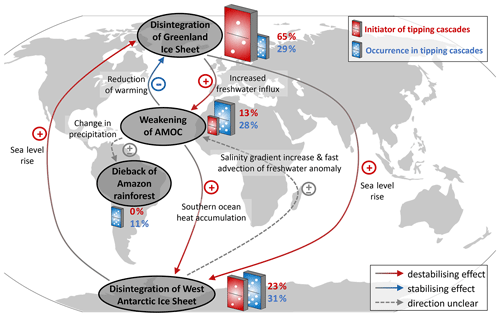
\includegraphics{fig/tipping_elements.png}

Risk increases significantly when considering interactions between these climate tipping elements and that these interactions tend to have an overall destabilising effect. Altogether, with the exception of the Greenland Ice Sheet, interactions effectively push the critical threshold temperatures to lower warming levels, thereby reducing the overall stability of the climate system. The domino-like interactions also foster cascading, non-linear responses. Under these circumstances, our model indicates that cascades are predominantly initiated by the polar ice sheets and mediated by the AMOC. Therefore, our results also imply that the negative feedback loop connecting the Greenland Ice Sheet and the AMOC might not be able to stabilise the climate system as a whole.

\href{https://esd.copernicus.org/articles/12/601/2021/}{Wunderling (2021) Interacting tipping elements increase risk of climate domino effects under global warming}

\href{https://www.theguardian.com/environment/2021/jun/03/climate-tipping-points-could-topple-like-dominoes-warn-scientists}{Guardian}

\hypertarget{tipping-points-in-clouds}{%
\section{Tipping Points in Clouds}\label{tipping-points-in-clouds}}

\emph{Johnson}

\textbf{Hysteresis}

The word ``hysteresis'' doesn't immediately seem threatening; it hints at a portmanteau of ``history'' and ``thesis''---a dense read, perhaps, but those never killed anyone. But that's not what the word means. Hysteresis is a profound behavior some systems can display, crossing a sort of point-of-no-return. Dial things up just one notch, and you can push the system through a radical change. To get back to normal, you might have to dial it down five or six notches.

Earth's climate system can provide examples. Take the conveyor-belt-like circulation of water in the Atlantic Ocean. Looking back at the past, you can see times that the circulation seems to have flipped into an alternate pattern regarding climatic consequences around the North Atlantic. Switching from one pattern to the other takes a significant nudge, but reversing it is hard---like driving up to the top of a ridge and rolling down into the next valley.

A new study led by Caltech's Tapio Schneider may have identified a disturbing hysteresis in Earth's climate---a shift in cloud patterns in response to warming that could quickly heat the planet much further. If we were to continue emitting more and more greenhouse gas, we'd eventually end up running this experiment for real. (Let's not, please.)

The center of this drama is a particular type of cloud. Stratocumulus clouds typically blanket about a fifth of the low-latitude ocean. Most clouds are formed because air warmed by the Earth's surface (or forced over mountains) cools as it rises, condensing water vapor to cloud droplets.

Stratocumulus clouds are a little different. The convection that lifts their moisture isn't driven by warming at the bottom but by cooling at the top.

The water in this cloud deck absorbs much of the infrared radiation emitted upward from the warm surface. The cloud deck re-emits some radiation back downward and some into outer space. The air above these clouds is drier and absorbs much less of the outgoing energy passing through it. That means you can think of these clouds like the cooling fins of a radiator. They shed more heat upward than they receive from the atmosphere above them, allowing them to cool off from the top down. The cold air at the top of the clouds sinks, setting up a convection loop that brings water vapor up from the sea surface to the cloud deck.

The key processes inside these stratocumulus cloud decks happen at a much, much smaller scale than a single grid cell in global climate models, so their physics aren't simulated directly. Instead, we have a simplified mathematical stand-in for their overall behavior. There is good reason to think this prevents us from understanding the details of how they'll respond to continued global warming.

To tackle this, Schneider and his colleagues flipped things around. They utilized a model that can simulate these clouds in a small patch of atmosphere---given a simplified version of the world around them. Specifically, they simulated a patch of the subtropical ocean with stratocumulus clouds above and a neighboring patch of tropical ocean responding to global warming. They did this for varying concentrations of greenhouse gas equivalent to 400 parts per million of CO2 (similar to today) on up to 1,600 parts per million.

Up to about 1,000 parts per million, there were no major surprises. Things got around 4°C warmer and numbers changed for things like water vapor and cloud altitude. But the cloud deck generally looked familiar.

At about 1,200 parts per million, however, the simulated clouds suddenly dissipated. And without that shade reflecting sunlight, the world warmed another 8°C.

How is CO2 flipping the switch on these clouds? The researchers found a pair of simple processes working together in their simulation. First, warmer air carries more water vapor up from the sea surface, and when that water vapor condenses, it releases a lot of latent heat. That extra latent heat gives the air a little buoyancy boost, increasing the turbulent movement that can mix dry air from above into the cloud layer. This dries out the cloud deck and makes cloud formation less likely.

Second, the increased CO2 (and water vapor) in the air above the cloud layer means that it absorbs more of the outgoing infrared radiation. Instead of pretty much staying out of the way and allowing the cloud layer to shed heat to space, the upper layer catches more and emits some back towards the clouds.

Both processes weaken the cloud deck, either by slowing the cooling-driven convection or by mixing in dry air. And in the model, the cloud deck just suddenly can't sustain itself anymore. It breaks up.

From there, the hysteresis is impressive. The warming that results from the loss of these clouds amplifies the processes that broke up the clouds in the first place. Dropping below 1,200 parts per million of CO2 again does not switch the clouds back on. Instead, the researchers had to bring it all the way down to 300 parts per million or so to see the cloud deck reform and stabilize.

It would take around a century of continued emissions growth to hit the equivalent of 1,200 parts per million CO2.

Some other projected trends in circulation would increase the stability of the cloud deck, allowing it to persist to higher CO2 concentrations. The model used in this study---which simplified the global picture to zoom in on one aspect---couldn't represent those processes. That means the exact numbers aren't the important thing here. The primary conclusion is that this sudden change in cloud behavior is possible

Climate models are often tested against past periods of climate change---and to study the causes of those climate changes. Efforts to simulate some very warm climates (like the Eocene 50 million years ago) have typically failed to get warm enough, though. To match the warmth indicated by geologic records, models have required higher CO2 than seems to have been present then. It could be that this is what the models are missing---a large temperature boost produced by a loss of marine cloud cover.

\href{https://arstechnica.com/science/2019/02/striking-study-finds-a-climate-tipping-point-in-clouds/}{Johnson (2022) Striking study finds a climate tipping point in clouds}

\emph{Schneider Abstract}

Stratocumulus clouds cover 20\% of the low-latitude oceans and are especially prevalent in the subtropics. They cool the Earth by shading large portions of its surface from sunlight. However, as their dynamical scales are too small to be resolvable in global climate models, predictions of their response to greenhouse warming have remained uncertain. Here we report how stratocumulus decks respond to greenhouse warming in large-eddy simulations that explicitly resolve cloud dynamics in a representative subtropical region. In the simulations, stratocumulus decks become unstable and break up into scattered clouds when CO2 levels rise above 1,200 ppm. In addition to the warming from rising CO2 levels, this instability triggers a surface warming of about 8 K globally and 10 K in the subtropics. Once the stratocumulus decks have broken up, they only re-form once CO2 concentrations drop substantially below the level at which the instability first occurred. Climate transitions that arise from this instability may have contributed importantly to hothouse climates and abrupt climate changes in the geological past. Such transitions to a much warmer climate may also occur in the future if CO2 levels continue to rise.

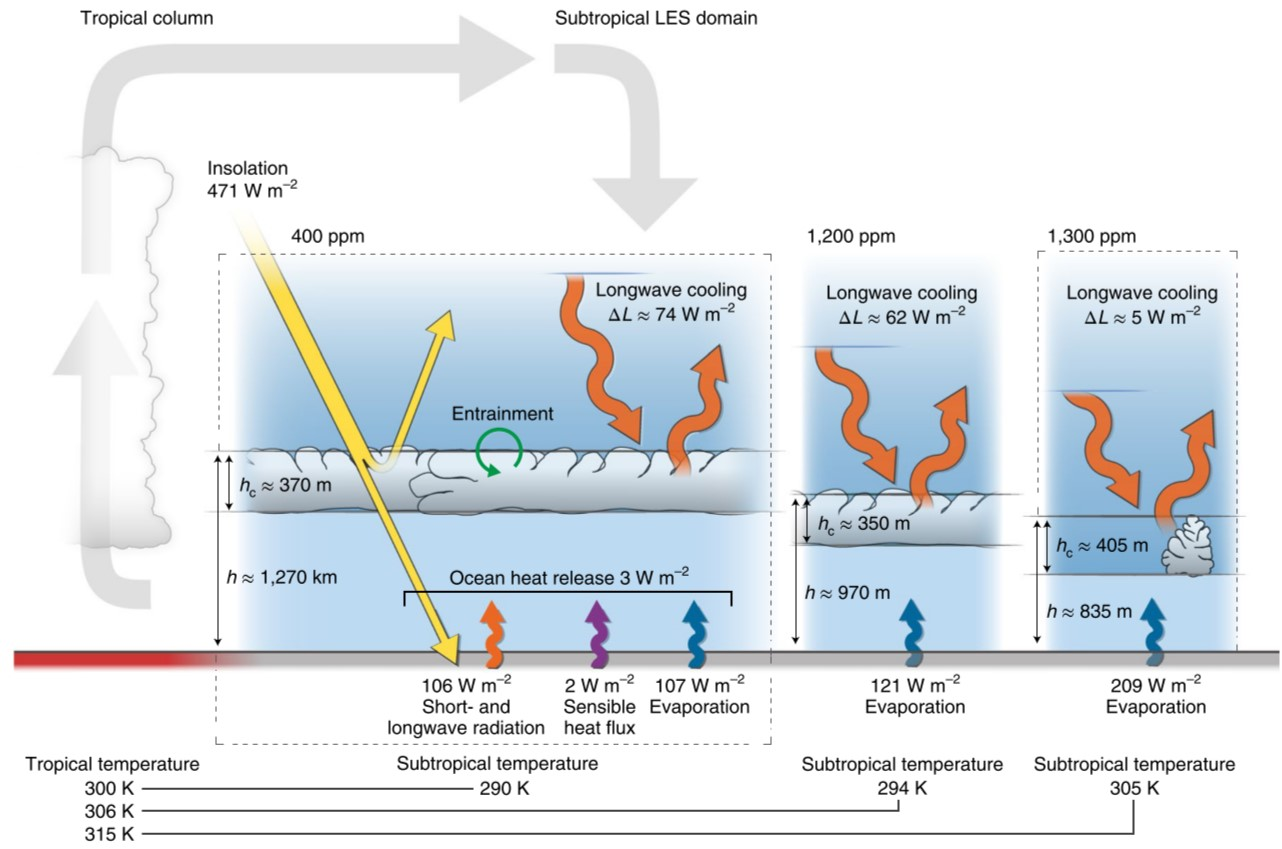
\includegraphics{fig/cloud_deck_breakup_at_1200ppm.jpg}

\emph{Fig. Simulated subtropical clouds in the present climate (400ppm CO2), at higher CO2 (1,200ppm) and after stratocumulus breakup (1,300ppm). In stratocumulus clouds, longwave radiative cooling of the cloud tops propels air parcels downward, which convectively connects the clouds to their moisture supply at the surface. Turbulence entrains warm and dry air across the inversion, which counteracts the radiative cooling and convective moistening of the cloud layer. When the atmospheric concentration of greenhouse gases (for example, CO2 and H2O) increases (1,200 ppm), the longwave cooling of the cloud tops weakens, because the downwelling longwave radiation that reaches the cloud tops from above emanates at lower levels with higher temperatures relative to the cloud-top temperatures. Eventually, at sufficiently high greenhouse gas concentrations (1,300 ppm in our simulation without subsidence changes), stratocumulus decks break up into cumulus clouds, which leads to dramatic surface warming. Evaporation then strengthens, and the average longwave cooling at the level of the cloud tops drops to less than 10\% of its value in the presence of stratocumulus decks.}

\href{https://www.nature.com/articles/s41561-019-0310-1.epdf?author_access_token=0KiqRkFsS6qEi37dkGz8X9RgN0jAjWel9jnR3ZoTv0Nq8LfnDsfOJgJee7VyE1P3etD8357qMjqyq2BVVSP5V9bFmsDkWYfYyGV7gtmSgJncc5u_hUNNfMaYS7BFcu8_tWNipaYj6kz2PMZ8OXu5CQ\%3D\%3D}{Schneider (2022) Possible climate transitions from breakup of stratocumulus decks under greenhouse warming}

\hypertarget{climate-change-indicators}{%
\chapter{Climate Change Indicators}\label{climate-change-indicators}}

\hypertarget{epa}{%
\section{EPA}\label{epa}}

EPA partners with more than 50 data contributors from various government agencies, academic institutions, and other U.S and international organizations to compile a key set of indicators related to the causes and effects of climate change.

\href{https://www.epa.gov/climate-indicators}{EPA Indicators}
\href{https://www.epa.gov/climate-indicators/frequent-questions-about-climate-change-indicators}{EPA Indicators FAQ}

EPA's climate change indicators are grouped into six categories:

\begin{verbatim}
[Greenhouse Gases](https://www.epa.gov/climate-indicators/greenhouse-gases)
[Weather and Climate](https://www.epa.gov/climate-indicators/weather-climate)
[Oceans](https://www.epa.gov/climate-indicators/oceans)
[Snow and Ice](https://www.epa.gov/climate-indicators/snow-ice)
[Health and Society](https://www.epa.gov/climate-indicators/health-society)
[Ecosystems](https://www.epa.gov/climate-indicators/ecosystems)
\end{verbatim}

\hypertarget{guardian}{%
\section{Guardian}\label{guardian}}

This page will track a selection of the planet's vital signs, from carbon dioxide levels to Arctic sea ice, and act as a reference point. The graphs are fed from data sources including Nasa, the US National Snow and Ice Data Center and the National Oceanic and Atmospheric Administration. They will automatically update and follow the Earth's climate trajectory, providing a visual representation of the climate crisis.

\href{https://www.theguardian.com/environment/ng-interactive/2020/oct/05/climate-data-dashboard-carbon-atmosphere-sea-level-arctic-ice}{Guardian Environment Interactive}

\hypertarget{ipcc}{%
\chapter{IPCC}\label{ipcc}}

\begin{quote}
The following phrase from the executive summary of Ch 10. of
the recent IPPC-2013 assessment (after stating that humans activities
extremely likely caused more than half of the observed GMTA increase)
might serve for summarising the actual situation:
``Uncertainties in forcings and in climate models' temperature responses
to individual forcings, and difficulty in distinguishing the patterns of
temperature response due to greenhouse gases and other anthropogenic
forcings prevent a more precise quantification of the temperature changes
attributable to greenhouse gases''.
\end{quote}

\begin{quote}
Therefore `detection' and `attribution' are still regarded as key
priorities in climate change research. IPCC defines `detection' as
the process of demonstrating that climate has changed in some statistical
sense, which means that the likelihood of occurrence by chance due to
internal variability alone is small.
\end{quote}

\begin{quote}
Besides statistical analysis of observed data, typically climate models
are used to predict the expected responses to external forcing and then
the consistency of this response pattern is evaluated with respect to
different components of the climate system
\end{quote}

As already noted in the Third Assessment Report 11 ,
`unequivocal attribution would require controlled experimentation
with the climate system.
Since that is not possible, in practice attribution of anthropogenic
climate change is understood to mean
demonstration that a detected change is
`consistent with the estimated responses to the given combination of
anthropogenic and natural forcing' and
`not consistent with alternative, physically plausible explanations of
recent climate change that exclude important
elements of the given combination of forcings.
Therefore attribution analysis is mainly performed through the
application of Global Circulation Models that allow
testing for causal relationships between anthropogenic forcing,
natural variability and temperature evolutions.
Pattern-based fingerprint studies provided strong scientific evidence of a
significant human influence on global atmospheric temperature changes.

\href{https://www.natur\%20e.com/articles/srep21691}{Stips (2016) On the causal structure between CO2 and global temperature}
\href{pdf/Stips_2016_Causal_structure_CO2_temperature.pdf}{(pdf)}

\hypertarget{shared-socioeconomic-pathways}{%
\section{Shared Socioeconomic Pathways}\label{shared-socioeconomic-pathways}}

The RCPs set pathways for greenhouse gas concentrations and, effectively, the amount of warming that could occur by the end of the century. Whereas the SSPs set the stage on which reductions in emissions will -- or will not -- be achieved.

The new SSPs offer five pathways that the world could take. Compared to previous scenarios, these offer a broader view of a ``business as usual'' world without future climate policy, with global warming in 2100 ranging from a low of 3.1C to a high of 5.1C above pre-industrial levels.

While the RCPs were finished in time to be used in the IPCC Fifth Assessment Report, developing the more complex SSPs has been a much longer and more involved process. The SSPs were initially published in 2016, but are only now just starting to be used in the next round of climate modelling -- known as the Coupled Model Intercomparison Project version 6, or CMIP6 -- in preparation for the IPCC's sixth assessment report.

The SSPs are based on five narratives describing broad socioeconomic trends that could shape future society. These are intended to span the range of plausible futures.

They include: a world of sustainability-focused growth and equality (SSP1); a ``middle of the road'' world where trends broadly follow their historical patterns (SSP2); a fragmented world of ``resurgent nationalism'' (SSP3); a world of ever-increasing inequality (SSP4); and a world of rapid and unconstrained growth in economic output and energy use (SSP5).

SSP1 Sustainability -- Taking the Green Road (Low challenges to mitigation and adaptation)
The world shifts gradually, but pervasively, toward a more sustainable path, emphasizing more inclusive development that respects perceived environmental boundaries. Management of the global commons slowly improves, educational and health investments accelerate the demographic transition, and the emphasis on economic growth shifts toward a broader emphasis on human well-being. Driven by an increasing commitment to achieving development goals, inequality is reduced both across and within countries. Consumption is oriented toward low material growth and lower resource and energy intensity.

SSP2 Middle of the Road (Medium challenges to mitigation and adaptation)
The world follows a path in which social, economic, and technological trends do not shift markedly from historical patterns. Development and income growth proceeds unevenly, with some countries making relatively good progress while others fall short of expectations. Global and national institutions work toward but make slow progress in achieving sustainable development goals. Environmental systems experience degradation, although there are some improvements and overall the intensity of resource and energy use declines. Global population growth is moderate and levels off in the second half of the century. Income inequality persists or improves only slowly and challenges to reducing vulnerability to societal and environmental changes remain.

SSP3 Regional Rivalry -- A Rocky Road (High challenges to mitigation and adaptation)
A resurgent nationalism, concerns about competitiveness and security, and regional conflicts push countries to increasingly focus on domestic or, at most, regional issues. Policies shift over time to become increasingly oriented toward national and regional security issues. Countries focus on achieving energy and food security goals within their own regions at the expense of broader-based development. Investments in education and technological development decline. Economic development is slow, consumption is material-intensive, and inequalities persist or worsen over time. Population growth is low in industrialized and high in developing countries. A low international priority for addressing environmental concerns leads to strong environmental degradation in some regions.

SSP4 Inequality -- A Road Divided (Low challenges to mitigation, high challenges to adaptation)
Highly unequal investments in human capital, combined with increasing disparities in economic opportunity and political power, lead to increasing inequalities and stratification both across and within countries. Over time, a gap widens between an internationally-connected society that contributes to knowledge- and capital-intensive sectors of the global economy, and a fragmented collection of lower-income, poorly educated societies that work in a labor intensive, low-tech economy. Social cohesion degrades and conflict and unrest become increasingly common. Technology development is high in the high-tech economy and sectors. The globally connected energy sector diversifies, with investments in both carbon-intensive fuels like coal and unconventional oil, but also low-carbon energy sources. Environmental policies focus on local issues around middle and high income areas.

SSP5 Fossil-fueled Development -- Taking the Highway (High challenges to mitigation, low challenges to adaptation)
This world places increasing faith in competitive markets, innovation and participatory societies to produce rapid technological progress and development of human capital as the path to sustainable development. Global markets are increasingly integrated. There are also strong investments in health, education, and institutions to enhance human and social capital. At the same time, the push for economic and social development is coupled with the exploitation of abundant fossil fuel resources and the adoption of resource and energy intensive lifestyles around the world. All these factors lead to rapid growth of the global economy, while global population peaks and declines in the 21st century. Local environmental problems like air pollution are successfully managed. There is faith in the ability to effectively manage social and ecological systems, including by geo-engineering if necessary.

The SSPs were designed to reflect worlds in which mitigation and adaptation challenges vary from low to very high. While the baseline SSP scenarios assume an absence of climate policy, researchers also wanted to look at how the underlying socioeconomic conditions would affect the implementation of climate policy.

For example, SSP1 features low challenges to mitigation and adaptation due to its rapid technological development, relative global equality of income and focus on environmental sustainability. SSP4, on the other hand, features similarly low challenges to mitigation due to its rapid technological development, but high challenges to climate adaptation due to persistent inequality and poverty in many parts of the world.

The main differences between SSPs come from their assumptions on global population growth, access to education, urbanisation, economic growth, resources availability, technology developments and drivers of demand, such as lifestyle changes.

All scenarios in the SSP database that keep warming below 2C incorporate some bioenergy with carbon capture and storage (BECCS).

\href{https://www.carbonbrief.org/explainer-how-shared-socioeconomic-pathways-explore-future-climate-change}{Hausfather (2018) SSP}

\hypertarget{part-measurements}{%
\part{Measurements}\label{part-measurements}}

\hypertarget{attribution}{%
\chapter{Attribution}\label{attribution}}

For too long, weather's randomness has kept events such as these from being blamed squarely on climate change. Reporters in the late 1990s and early 2000s would ask climate scientists about climate change's role in a weather-related disaster. All we could say was that we'd expect to see more of these events. Now, we can specify increased chances for specific events. This extends to forecasts: we can identify the places that are more likely to see wildfires, mudslides and fish die-offs. Such calculations dent both climate denial and a false sense of security. They take away the argument that `extreme weather happens anyway, so we don't need to worry about it'. Extreme weather happens --- and these metrics pinpoint what is becoming more likely, by how much and why.

\href{https://www.nature.com/articles/d41586-021-00185-x}{Betts (2021) Nature}

\href{https://www.ametsoc.org/ams/index.cfm/publications/bulletin-of-the-american-meteorological-society-bams/explaining-extreme-events-from-a-climate-perspective/}{Ametsoc (2021) Explaining Extreme Weather}
\href{pdf/Ametsoc_2021_Explaining_Extreme_2019.pdf}{(pdf)}

\hypertarget{attribution-studies-timeline}{%
\section{Attribution Studies Timeline}\label{attribution-studies-timeline}}

\emph{ClimateChangeNews}

AR5 concluded that human influence on the climate system is ``clear.'' Today scientists say climate change is, without doubt, caused by us. A 2021 \href{https://www.nature.com/articles/s41558-020-00965-9}{study} concluded that humans have caused all of the warming observed since the preindustrial period.

Since the last IPCC report, there has been an explosion of attribution studies finding that specific heatwaves, droughts, tropical cyclones and other extreme events were more likely or intense because of climate change. Recent studies have shown that extreme events such as the Siberian heat wave in 2020 would never have happened without humans pumping greenhouse gases into the air.

Since AR5, attribution science has become more ``impact-oriented'', Sjoukje Philip, a climate scientist from the World Weather Attribution (WWA) group, told Climate Home News.
That means more studies focusing on the societal impacts of extreme weather events.

The increase in attribution studies is due to more precise climate models and peer-reviewed methods which allow scientists to rapidly and accurately analyse extreme events.
Scientists are now able to carry out attribution studies within a few days of an event occurring.

Half of all attribution studies focus on heatwaves.
Heatwaves are relatively easy to attribute because they are ``very certain and the first response to climate change'' and cover a large area, which makes it easier for climate models to pick up.
Most of the rest look at extremes of rainfall leading to drought or floods.
Only a handful have looked at hurricanes, which are hard to model due to their complexity and limited historical data. They reached relatively weak conclusions about the scale of human influence.
That could change as new high-resolution models are being developed.

The majority of attribution studies focus on events in Europe and North America. This is because these regions have the most reliable climate data available.

\textbf{Timeline of climate attribution studies}

2004: First heatwave attribution study

The study found that climate change had at least doubled the likelihood of the European heatwave in 2003, which killed more than 70,000 people.

2011: First flooding attribution study

The first study to attribute greenhouse gas emissions' contribution to flood risk in England and Wales. The scientists concluded that emissions increased the risk of floods occurring in England and Wales in autumn 2000 by more than 20\% and in two out of three cases by more than 90\%.

2014: Likelihood of European heatwaves analysis

The study found that summer heatwaves in Europe over the past 10-15 years were 10 times more likely due to climate change

2016: Mortality study of European heatwave

The first study to directly link deaths during the 2003 European heatwave to climate change. The scientists concluded that 506 of the 735 summer fatalities in Paris in 2003, and 64 of the 315 in London were a result of climate change.

2017: Bangladesh flooding study

World Weather Attribution analysis directly linked severe flooding in Bangladesh in 2017 to climate change.

2018: Cape Town water crisis analysis

The 2017 drought which led to Cape Town's water crisis was made three times more likely by climate change, according to analysis by World Weather Attribution scientists.

2018: Extreme heat across Asia

Extreme heat across Asia in 2016 would have been impossible without climate change, scientists concluded in 2018.

2020: Siberian heatwave impossible without climate change

The prolonged Siberian heatwave in 2020 would have been almost impossible without climate change, according to rapid attribution analysis by the World Weather Attribution group.

2021: Australian bushfire season 30\% more likely

Australia's devastating bushfire season in 2019-202 was made significantly more likely because of climate change, according to World Weather Attribution scientists. The analysis showed that climate change led to weather conditions that increased the fire risk by at least 30\%.

\href{https://www.climatechangenews.com/2021/08/04/timeline-science-linking-climate-change-extreme-weather-took-off/}{ClimateChangeNews}

\hypertarget{map-of-attribution-studies}{%
\section{Map of Attribution Studies}\label{map-of-attribution-studies}}

Known as ``extreme event attribution'', the field has gained momentum, not only in the science world, but also in the media and public imagination. These studies have the power to link the seemingly abstract concept of climate change with personal and tangible experiences of the weather.

Scientists have published more than 300 peer-reviewed studies looking at weather extremes around the world, from wildfires in Alaska (pdf) and hurricanes in the Caribbean to flooding in France and heatwaves in China. The result is mounting evidence that human activity is raising the risk of some types of extreme weather, especially those linked to heat.

To track how the evidence on this fast-moving topic is stacking up, Carbon Brief has mapped -- to the best of our knowledge -- every extreme-weather attribution study published to date.

The map above shows 355 extreme weather events and trends across the globe for which scientists have carried out attribution studies.

\href{https://www.carbonbrief.org/mapped-how-climate-change-affects-extreme-weather-around-the-world}{Carbon BriefMap}

\hypertarget{bottom-trawling-co2-release}{%
\section{Bottom Trawling CO2 release}\label{bottom-trawling-co2-release}}

\emph{Time Magzine: How Industrial Fishing Creates More CO2 Emissions Than Air Travel}

Bottom trawling is responsible for one gigaton of carbon emissions a year---a higher annual total than (pre-pandemic) aviation emissions. Not only does the practice contribute to climate change, it is extremely damaging to ocean biodiversity---the ``equivalent of ploughing an old-growth forest into the ground, over and over and over again until there is nothing left''

Bottom trawling is also one of the least cost effective methods of fishing. Most locations have been trawled so many times, there is little left worth catching.
Without government subsidies, no one would be making a penny.

Refuting a long-held view that ocean protection harms fisheries, the study found that well placed marine protected areas (MPAs) that ban fishing would actually boost the production of marine life by functioning as fish nurseries and biodiversity generators capable of seeding stocks elsewhere.

\emph{Sala}

Marine sediments are the largest pool of organic carbon on the planet and a crucial reservoir for long-term storage29. If left undisturbed, organic carbon stored in marine sediments can remain there for millen-nia30. However, disturbance of these carbon stores can re-mineralize sed-imentary carbon to CO2, which is likely to increase ocean acidification, reduce the buffering capacityof the ocean and potentially add to the build-up of atmospheric CO2

Using satellite-inferred information on fishing activity by industrial trawlers and dredgers between 2016 and 2019, aggregated at a reso-lution of 1km2, we estimate that 4.9million km2 or 1.3\% of the global ocean is trawled each year. This disturbance to the seafloor results in an estimated 1.47Pg of aqueous CO2 emissions, owing to increased carbon metabolism in the sediment in the first year after trawling. If trawling continues in subsequent years, emissions decline as sediment
carbon stocks become exhausted. However, after 9 years of continuous trawling, emissions stabilize at around 40\% of the first year's emissions, or around 0.58Pg CO2 (Supplementary Fig.35). If the intensity and footprint of trawling remains constant, we estimate that sediment carbon emissions will continue at approximately 0.58Pg CO2 for up to around 400 years of trawling, after which all of the sediments in the top metre are depleted. Although 1.47Pg CO2 represents only 0.02\% of total marine sedimentary carbon, it is equivalent to 15--20\% of the atmospheric CO2 absorbed by the ocean each year32,33, and is compara-ble to estimates of carbon loss in terrestrial soils caused by farming34. Although an unknown fraction of the aqueous CO2 is emitted to the atmosphere, the increase in CO2 in the water column and sediment pore waters can have far-reaching and complex effects on marine carbon cycling, primary productivity and biodiversity.

\href{https://time.com/5947430/bottom-trawling-carbon-emissions-study/}{Time Magzine}
\href{https://www.bbc.com/news/science-environment-56430542}{BBC}
\href{https://www.nature.com/articles/s41586-021-03371-z.epdf?sharing_token=6Sow3BIdqBYvlWAiGEDpk9RgN0jAjWel9jnR3ZoTv0MwjSp_dqdYRo11ccDn9dqPW5D1xJuK8fpT__q4KFNUwr3chDwJyG9IO5W1aWFy5onfZKtxUPkvQTnzNtoVopyg-N66E6j3SdEzqNh2UnnVHpANtYD9CYy7I3QNIz6iI184RD1jaDt2fU8Yl8bdsQppKG7J6tfBiSTN74eTrygUTMPeqTv4M1289Ys38rtf2Cu5Gfo8iuQxzcCwuSri_N3NIdmY-iR2Af8IOP_F9-p_RA\%3D\%3D\&tracking_referrer=time.com}{Sala (2021) Protecting the global ocean for biodiversity, food and climate - Nature Share}

\hypertarget{company-attribution}{%
\section{Company Attribution}\label{company-attribution}}

A 2017 report by the Carbon Disclosure Project showed that 100 companies have been responsible for 71 per cent of global emissions since 1988. In 2019, a similar study from the Climate Accountability Institute found that just 20 companies were responsible for 35 per cent of all energy-related carbon dioxide and methane worldwide since 1965.

\href{https://tribunemag.co.uk/2021/03/paper-straws-are-not-enough}{Sultana}

\hypertarget{carbon-budget}{%
\chapter{Carbon Budget}\label{carbon-budget}}

\begin{quote}
The temperature response for a 1.5°C scenario has a huge uncertainty \& this propagates to the uncertainty in the carbon budget.
To say ``the remaining carbon budget for 1.5°C is 440 GtCO₂'' {[}add favorite number{]} is highly misleading
Taking a narrow 67--33\% range, the value is 230--670 GtCO₂, but full range (left) could be −1000 - 2000 GtCO₂\ldots{} (yes, could be negative or huge)
(Glen Peters)
\end{quote}

\emph{Memo Matthews:}

The remaining carbon budget quantifies the future CO 2 emissions to limit global warming
below a desired level. Carbon budgets are subject to uncertainty in the Transient Climate
Response to Cumulative CO 2 Emissions (TCRE), as well as to non-CO 2 climate influences.
We estimate a median TCRE of 0.44 °C and 5--95\% range of 0.32--0.62 °C per 1000 GtCO 2
emitted. Considering only geophysical uncertainties, our median estimate of the 1.5 °C
remaining carbon budget is 440 GtCO 2 from 2020 onwards, with a range of 230--670
GtCO 2 , (for a 67--33\% chance of not exceeding the target). Additional socioeconomic
uncertainty related to human decisions regarding future non-CO 2 emissions scenarios can
further shift the median 1.5 °C remaining carbon budget by ±170 GtCO 2 .

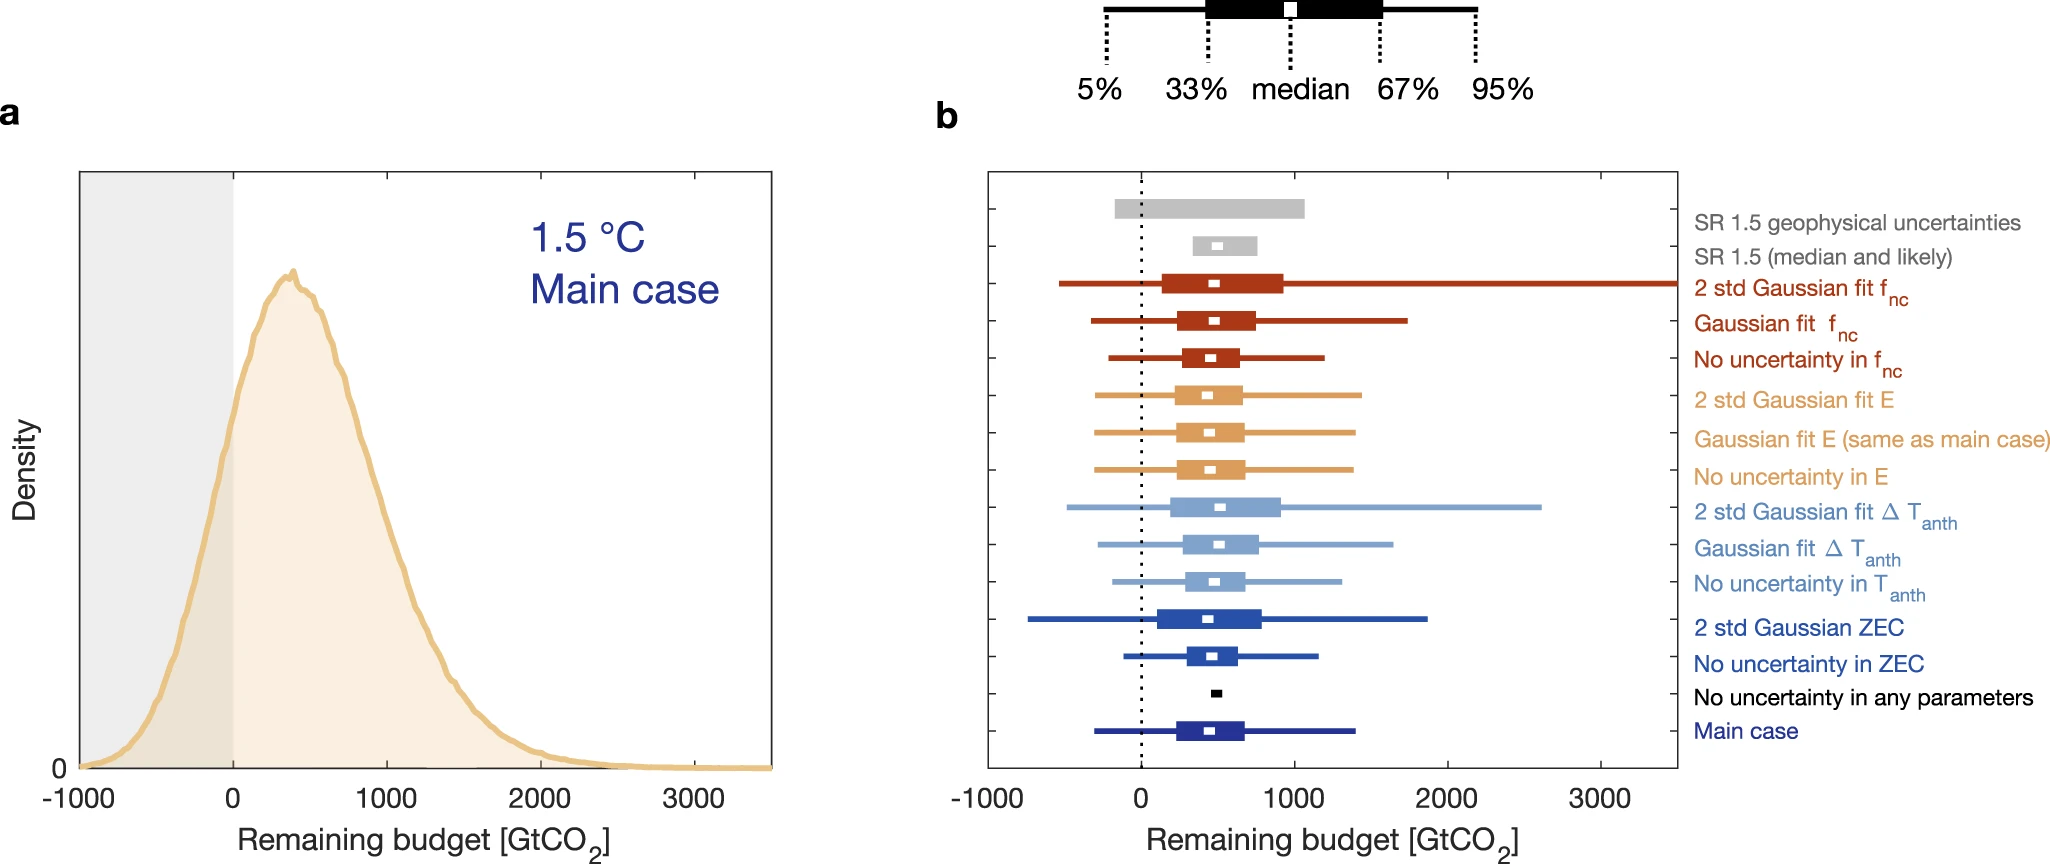
\includegraphics{fig/carbon_budget.png}

Remaining carbon budgets (RCBs) represent the future
cumulative CO 2 emissions that would be consistent with
keeping global warming to a specified level.
Despite being conceptually simple, RCBs have been
defined and estimated in various ways and with many different
underlying assumptions, resulting in a wide range of
``best estimates'' across different studies 2 . Moreover, most of these
estimates of remaining budgets account for only a subset of the
relevant uncertain processes and often omit the contribution of
key uncertain processes (such as permafrost thaw or future
scenario uncertainty, among others)

Median TCRE estimate is 0.44 °C per 1000 GtCO2 , with a 5--95\%
range of 0.32--0.62 °C per 1000 GtCO2

A stronger constraint on the left-hand side of the distribution (low
TCRE values, with sharply increasing probability above 0.25 °C/
1000 GtCO 2 ), while the right-hand side of this distribution has a
wider tail. This right-skewed distribution shape of our
observationally-constrained TCRE estimate is physically related
to the possibility of a large negative aerosol forcing

Median RCB for 1.5 °C is 440 GtCO2 from 2020
onwards, representing a 50\% chance of stabilising warming at or
below 1.5 °C.
The corresponding budget for a 67\% chance of remaining below the target is
230 GtCO2 from the year 2020 onwards.

\href{https://www.nature.com/articles/s43247-020-00064-9}{Matthews(2021) Carbon Budget Uncertainties}
\href{pdf/Matthews_2021_Carbon_Budget_Uncertainties.pdf}{(pdf)}

\hypertarget{net-zero}{%
\section{Net-zero}\label{net-zero}}

\emph{Disaster looms if big finance is allowed to game the carbon offsetting markets to achieve `net zero' emissions.}

\emph{Net zero increasingly involves highly questionable carbon accounting. As a result, the new politics swirling around net zero targets is rapidly becoming a confusing and dangerous mix of pragmatism, self-delusion and weapons-grade greenwash.}

The science of net zero is simple: every sector of every country in the world needs to be, on average, zero emissions. We know how to do this for electricity, cars, buildings and even a lot of heavy industry. But in certain areas, including air travel and some agricultural emissions, there is no prospect of getting to zero emissions in the near future. For these residual emissions, greenhouse gasses will need to be sucked out of the atmosphere at the same rate as they are added, so that, on average, there are net zero emissions.

The science of net zero is simple: every sector of every country in the world needs to be, on average, zero emissions. We know how to do this for electricity, cars, buildings and even a lot of heavy industry. But in certain areas, including air travel and some agricultural emissions, there is no prospect of getting to zero emissions in the near future. For these residual emissions, greenhouse gasses will need to be sucked out of the atmosphere at the same rate as they are added, so that, on average, there are net zero emissions.

Making this work requires carbon removal, also known as ``negative emissions''. This can be low-tech, like restoring forests, as this takes carbon out of the atmosphere and stores it in trees. Or it can be hi-tech, like using chemicals to strip carbon dioxide from the atmosphere and then pumping it deep underground into safe geological storage. In theory this is all fine, as pragmatically some carbon removal is needed to balance hard-to-reduce emissions: but negative emissions and offsetting alone are not a route to net zero.

In practice, by believing in the promise of these methods, we are too often deceiving ourselves, in three major ways. The first is an unrealistic overreliance on carbon removal to preserve the status quo.
Critically, there is far too little land to plant enough trees to counter today's emissions, and large-scale hi-tech methods do not yet exist.
The second deception is in offsetting against notional emissions trajectories instead of removing carbon from the atmosphere.Offsetting needs to be used to remove carbon dioxide from the atmosphere to counter difficult-to-remove emissions, and not just be an enabler of business-as-nearly-usual.
The third deception comes from not getting what you think you're paying for in the self-regulated global carbon market. The commercial carbon offset concept relies on ``additionality'' -- that money paid then reduces emissions or captures carbon that would not otherwise have happened.
The offsets market is awash with old legacy carbon credits where that assumption is violated.

If such deceptions remain, disaster looms. Big finance, led by Carney, is planning to massively expand carbon markets. Conceivably, new carbon-based financial products could boom, with little impact on emissions. Just like the sub-prime crisis, few will understand what they bought, and another globe-spanning crash could sweep the world, compounding economic and climate crises causing mass suffering, as we realise again that the Earth owes us nothing. Nature doesn't do bailouts.

\href{https://www.theguardian.com/commentisfree/2021/mar/03/climate-crisis-carbon-accounting-tricks-big-finance}{Lewis (Guardian)}

\hypertarget{revelle-factor}{%
\section{Revelle factor}\label{revelle-factor}}

\emph{Wikipedia}

The Revelle factor (buffer factor) is the ratio of instantaneous change in carbon dioxide (CO
2) to the change in total dissolved inorganic carbon (DIC), and is a measure of the resistance to atmospheric CO2 being absorbed by the ocean surface layer.{[}1{]} The buffer factor is used to examine the distribution of CO2 between the atmosphere and the ocean, and measures the amount of CO2 that can be dissolved in the mixed surface layer. It is named after the oceanographer Roger Revelle. The Revelle factor describes the ocean's ability to uptake atmospheric CO2, and is typically referenced in global carbon budget analysis and anthropogenic climate change studies.

In order to enter the ocean, carbon dioxide gas has to partition into one of the components of carbonic acid: carbonate ion, bicarbonate ion, or protonated carbonic acid, and the product of these many chemical dissociation constants factors into a ``back-pressure'' that limits how fast the carbon dioxide can enter the surface ocean.

The capacity of the ocean waters to take up surplus (anthropogenic) CO2 is inversely proportional to the value of the Revelle factor. Hence, in modern-day oceans, it is possible to see the concentrations of anthropogenic CO2 by measuring the Revelle factor; the lower the Revelle factor, the greater the amount of anthropogenic CO2.{[}4{]} Low Revelle factors are typically found in the warmer tropical to subtropical waters, whereas higher Revelle factors are found in the colder high latitude waters of the North Atlantic. The North Pacific has higher Revelle factors, and has lower anthropogenic CO
2. This is due to the fact that the alkalinity values in the North Pacific are as much as 100μmol/kg lower than those in the North Atlantic.

The Revelle effect describes how only a small fraction of pCO2 is present in ocean water when much larger amounts are added to the atmosphere. Depending on the alkalinity of the water, DIC is either present as CO3, HCO3, or CO2. When the pH is high (basic) the Revelle factor is greatest, causing much of the DIC to exist as HCO3 or CO3, and not CO2. So, the greater the buffering effect (low Revelle Factor) the more DIC occurs as CO3 or HCO3, effectively lowering the pCO2 levels in both the atmosphere and ocean.

\href{https://en.wikipedia.org/wiki/Revelle_factor}{Wikipedia Revelle Factor}

\hypertarget{climate-sensitivity}{%
\chapter{Climate Sensitivity}\label{climate-sensitivity}}

\hypertarget{climate-feedbacks}{%
\section{Climate Feedbacks}\label{climate-feedbacks}}

\emph{Abstract Heinze}
Earth system models (ESMs) are key tools for providing climate projections under different sce-
narios of human-induced forcing. ESMs include a large number of additional processes and feedbacks such as
biogeochemical cycles that traditional physical climate models do not consider. Yet, some processes such as
cloud dynamics and ecosystem functional response still have fairly high uncertainties. In this article, we present
an overview of climate feedbacks for Earth system components currently included in state-of-the-art ESMs and
discuss the challenges to evaluate and quantify them. Uncertainties in feedback quantification arise from the in-
terdependencies of biogeochemical matter fluxes and physical properties, the spatial and temporal heterogeneity
of processes, and the lack of long-term continuous observational data to constrain them. We present an outlook
for promising approaches that can help to quantify and to constrain the large number of feedbacks in ESMs in
the future. The target group for this article includes generalists with a background in natural sciences and an
interest in climate change as well as experts working in interdisciplinary climate research (researchers, lecturers,
and students). This study updates and significantly expands upon the last comprehensive overview of climate
feedbacks in ESMs, which was produced 15 years ago (NRC, 2003).

\href{https://www.researchgate.net/publication/334387499_ESD_Reviews_Climate_feedbacks_in_the_Earth_system_and_prospects_for_their_evaluation}{Heinze (2019) Climate Feedbacks}
\href{pdf/Heinze_2019_Climate_Feedbacks.pdf}{(pdf)}

\hypertarget{ecs---equilibrium-climate-sensitivity}{%
\section{ECS - Equilibrium Climate Sensitivity}\label{ecs---equilibrium-climate-sensitivity}}

\emph{ECS}

Climate sensitivity is defined as the equilibrium change in global and annual mean
surface air temperature, \(\Delta T\), due to an increment in
downward radiative flux, \(\Delta R_{f}\) ,
that would result from sustained doubling of atmospheric \(CO_2\) over its
preindustrial value (2 x \(CO_2\) ).

Studies based, on observations, energy balance models, temperature reconstructions,
and global climate models (GCMs) have found that the probability
density distribution of \(\Delta T\) is peaked in the range
2.0°C ≤ \(\Delta T\) ≤ 4.5°C, with a long tail of small but
finite probabilities of very large temperature increases.

An important parameter in climate science is
the equilibrium or long-run response in the global mean surface temperature
to a doubling of atmospheric carbon dioxide.

In the climate science community, this is called
the equilibrium climate sensitivity ECS.
With reference to climate models, this is calculated as
the increase in average surface temperature with a doubled CO2 concentration
relative to a path with the pre-industrial CO2 concentration.
This parameter also plays a key role in the geophysical components
in the IAMs.

Given the importance of the ECS in climate science,
there is an extensive literature estimating probability density functions.
These pdfs are generally based on climate models, the instrumental
records over the last century or so, paleoclimatic data such
as estimated temperature and radiative forcings over ice-age intervals,
and the results of volcanic eruptions.
Much of the literature estimates a probability density function
using a single line of evidence,
but a few papers synthesize different studies or different kinds of evidence.

The IPCC Fifth Assessment report (AR5) reviewed the literature
quantifying uncertainty in the ECS and highlighted
five recent papers using multiple lines of evidence (IPCC, 2014).
Each paper used a Bayesian approach to update a prior distribution
based on previous evidence
(the prior evidence usually drawn from instrumental records or a climate model)
to calculate the posterior probability density function.

\href{https://globalchange.mit.edu/publication/16235}{Gilligham (2015) Modelling Uncertainty}
\href{pdf/Gillingham_2015_Modelling_Uncertainty.pdf}{(pdf)}

\hypertarget{roe-and-baker-distribution}{%
\subsection{Roe and Baker Distribution}\label{roe-and-baker-distribution}}

\emph{Abstract}

Uncertainties in projections of future climate change have not lessened substantially in past
decades. Both models and observations yield broad probability distributions for long-term
increases in global mean temperature expected from the doubling of atmospheric carbon dioxide,
with small but finite probabilities of very large increases. We show that the shape of these
probability distributions is an inevitable and general consequence of the nature of the climate
system, and we derive a simple analytic form for the shape that fits recent published distributions
very well. We show that the breadth of the distribution and, in particular, the probability of
large temperature increases are relatively insensitive to decreases in uncertainties associated with
the underlying climate processes.

\emph{Memo Roe and Baker}

What determines the distribution shape of ECS and in particular, the high \(\Delta T\) tail?
To what extent we can decrease the distribution width?

Climate consists of a set of highly coupled, tightly interacting physical processes.
Understanding these physical processes is a massive
task that will always be subject to uncertainty.
How do the uncertainties in the physical processes translate into an uncertainty in climate
sensitivity?

Explanations for the range of
predictions of DT, summarized in (14), have
focused on
(i) uncertainties in our understanding of the individual physical processes
(in particular, those associated with clouds),
(ii) complex interactions among the individual processes, and
(iii) the chaotic, turbulent nature of the climate system, which may give rise to
thresholds, bifurcations, and other discontinuities, and which
remains poorly understood on a theoretical level.
We show here that the explanation is far more fundamental than any of these.

We use the framework of feedback analysis to examine the relationship between the
uncertainties in the individual physical processes and the ensuing shape of
the probability distribution of \(\Delta T\).
Because we are considering an equilibrium temperature rise, we consider only
time-independent processes.

\href{https://www.semanticscholar.org/paper/Why-Is-Climate-Sensitivity-So-Unpredictable-Roe-Baker/9a0c81f6887db897000dbce576b139a486f62c77}{Roe and Baker (2007) Climate Sensitivity}
\href{pdf/Roe_Baker_2007_Climate_Sensitivity.pdf}{(pdf)}

\emph{Memo Hannart}

RB addressed these questions using rather simple
theoretical considerations and reached the conclusion that
reducing uncertainties on climate feedbacks and underlying
climate processes will not yield a large reduction in the
envelope of climate sensitivity. In this letter, we revisit the
premises of this conclusion. We show that it results from a
mathematical artifact caused by a peculiar definition of
uncertainty used by these authors.

Reducing inter-model spread on
feedbacks does in fact induce a reduction of uncertainty on
climate sensitivity, almost proportionally.
Therefore, following Roe and Baker assumptions, climate sensitivity is actually
not so unpredictable.

The main originality of RB07 approach consists in analyzing
explicitly the way uncertainties on \(f\), due to a limited
understanding of their underlying physical processes, prop-
agates into uncertainties on \(\Delta T\): assuming \(f\) is a random
variable with mean \(f\) and standard deviation \(\sigma_f\) , RB07 uses
this simple probabilistic model to highlight several fundamental
properties of uncertainty propagation from feedbacks
to climate sensitivity. The most prominent conclusion of this
analysis is that reducing uncertainties on \(f\) does not yield a
large reduction in the uncertainty of \(\Delta T\), and thus that
improvements in the understanding of physical processes
will not yield large reductions in the envelope of future
climate projections.
We show that this conclusion is a mathematical artifact
with no connection whatsoever to climate.

RB07 uses the feedback analysis framework.
Denoting \(\Delta T_0\) the Planck temperature response to the radiative
perturbation and \(f\) the feedback gain (RB07 refers to it as
feedback factor), they obtain:

\[\Delta T = \frac{\Delta T_0}{1 - f}\]

RB07 then assumes uncertainty on Planck response to be
negligible so that the entire spread on \(\Delta T\) results from the
uncertainty on the global feedback gain \(f\). To model this
uncertainty, RB07 assumes that \(f\) follows a Gaussian
distribution with mean \(\overline{f}\) , standard deviation \(\sigma_f\) and implicit
truncation for \(f\) \textgreater{} 1.
Then, they derive an exact expression of the distribution of \(\Delta T\).
This simple probabilistic climatic model is used by RB07 to analyze the
way uncertainties on \(f\), due to a limited understanding of
underlying physical processes, propagates into uncertainties
on \(\Delta T\). Their analysis highlights two fundamental properties:

\begin{enumerate}
\def\labelenumi{\arabic{enumi}.}
\item
  \emph{Amplification}: The term in \(\frac{1}{1-f}\)
  amplifies uncertainty on feedbacks, all the more intensely as
  \(f\) is close to (though lower than) one. Small uncertainties on
  feedbacks are thus converted in large uncertainties on the
  rise of temperature.
\item
  \emph{Insensitivity}: reducing uncertainty on \(f\) has
  little effect in reducing uncertainty on \(\Delta T\),
  also stated as the breadth of the distribution of \(\Delta T\)
  is relatively insensitive to decreases in \(\sigma_f\).
\end{enumerate}

We are puzzled by the second property, that is,
the claimed insensitivity of uncertainty on \(\Delta T\) to uncertainty on feedbacks.
The reason why one may find this second assertion puzzling,
is that it intuitively seems to contradict the first.

While the probability \(P(\Delta T \in [4.5°C, 8°C])\) may be of interest practically,
this metric is irrelevant to describe \emph{the breadth of the
distribution of climate sensitivity} which was RB07 explicit intent.
To address this question, any measure of distribution
spread chosen amongst those classically used in Descriptive
Statistics is more appropriate.

(Hugo Mathjax don't render correctly here:?? OK in rpad !! OK in mathjaxtest!!)
With such measures when the spread of feedback parameter \(S_f\) decreases,
the resulting spread of climate sensitivity \(S_{\Delta T}\) values also decreases.
Further the decrease is approximately linear for
\(S_f\) small and tends to be steeper for larger values of \(S_{f}\) .

\href{https://agupubs.onlinelibrary.wiley.com/doi/full/10.1029/2009GL039640}{Hannart on RB}
\href{pdf/Hannart_2009_ECS_not_so_Unpredictable.pdf}{(pdf)}

\href{https://github.com/rtol/roebaker}{Tol: RB-fitting Github}

\emph{Memo Jules and James}
Roe and Baker have attempted to justify the pdfs that have been generated
as not only reasonable, but inevitable on theoretical grounds

RB's basic point is that if ``feedback'' \(f\) is considered to be Gaussian, then
sensitivity = \(\lambda_0/(1-f)\) is going to be skewed, which seems fair enough.

Where I part company with them is when they claim that this gives rise to some
fundamental and substantial difficulty in generating more precise estimates
of climate sensitivity, and also that it explains
the apparent lack of progress in improving on the long-standing
1979 Charney report estimate of 1.5-4.5C at only the ``likely'' level.

Stoat's complaints also seem pertinent:
\(f\) cannot really be a true Gaussian,
unless one is willing to seriously consider large negative sensitivity,
and even though a Gaussian is a widespread and often reasonable distribution,
it is hard to find any theoretical or practical basis for
a Gaussian abruptly truncated at 1.

I can think of several alternative theories as to
why the uncertainty in the IPCC estimate has not reduced.
The probabilistic methods generally used to generate these long-tailed pdfs
are essentially pathological in their use of a uniform prior
(under the erroneous belief that this represents ``ignorance''),
together with only looking at one small subset of the pertinent data at a time,
and therefore do not give results that can credibly represent
the opinions of informed scientists.

There may also be the sociological effect of this range as some sort of anchoring device, which people are reluctant to change despite its rather shaky origins. Ramping up uncertainty (at least at the high end) is a handy lever for those who argue for strong mitigation, and it would also be naive to ignore the fact that scientists working in this area benefit from its prominence.

\href{http://julesandjames.blogspot.com/2007/10/roe-and-baker.html}{Jules and James: Comment on RB}

\emph{Memo Gillingham}

Note that the US government used a version of the Roe and Baker distribution
calibrated to three constraints from the IPCC
for its uncertainty estimates (IAWG, 2010).
Specifically, the IAWG Report modified the original Roe and Baker distribution
to assume that the median value is 3.0°C,
the probability of being between 2 and 4.5°C is two-thirds,
and there is no mass below zero or above 10°C.
The modified Roe and Baker distribution has a higher mean ECS than
any of the models (3.5°C) and
a much higher dispersion (1.6°C as compared to 0.84°C from Olsen et al.~2012).

\href{https://globalchange.mit.edu/publication/16235}{Gilligham (2015) Modelling Uncertainty}
\href{pdf/Gillingham_2015_Modelling_Uncertainty.pdf}{(pdf)}

\hypertarget{gcm-based-approach}{%
\subsection{GCM based Approach}\label{gcm-based-approach}}

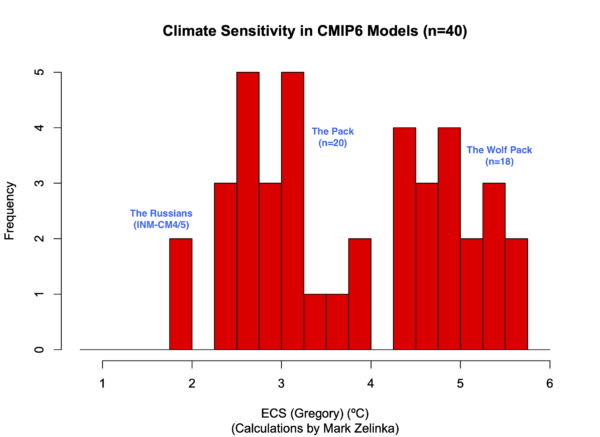
\includegraphics{fig/Gavin_2020_cmip6_ecs.png}

\href{http://www.realclimate.org/index.php/archives/2019/11/sensitive-but-unclassified/}{Gavin (2019) RealClimate (Part 1)}

\href{http://www.realclimate.org/index.php/archives/2020/06/sensitive-but-unclassified-part-ii/}{Gavin (2020) RealClimate (Part 2)}

\hypertarget{gcm-free-approach}{%
\subsection{GCM free Approach}\label{gcm-free-approach}}

\emph{Memo}

\begin{itemize}
\tightlist
\item
  GCM free approach
\end{itemize}

The atmosphere is a complex system involving turbulent
processes operating over a wide range of scales starting
from millimeters at the Kolmogorov dissipation scale up
to the size of the Earth, spanning over 10 orders of magni-
tudes in space.

The dynamics are sensitive to initial conditions and there are
deterministic predictability limits that
are roughly equal to the eddy turn-over time (lifetime) of
structures.

For planetary scale structures in the atmosphere,
the overall deterministic prediction limit of about 10 days
corresponds to the scaling transition timescale τ w from the
weather regime to the macroweather regime.

The atmospheric components of GCMs exhibit the same
weather-macroweather scaling transition as the atmosphere
and similar predictability limits. Beyond this horizon, the
internal variability has to be interpreted stochastically so
that a single GCM run is only one realization of the random
process; at these timescales, weather models effectively
become stochastic macroweather generators. For projec-
tions over multi-decadal timescales and beyond, multi-model
ensembles (MME) that include several models are used. The
mean of the MME is taken to obtain the deterministic forced
component of temperature variability and average out the
internal variability (Collins et al.~2013).

Emergent properties of the Earth's climate, i.e.~proper-
ties which are not specified a priori, are then inferred from
GCM simulations.

The equilibrium climate sensitivity (ECS)
is such a property; it refers to the expected temperature
change after an infinitely long time following a doubling in
carbon dioxide ( CO 2 ) atmospheric concentration.

Another is the transient climate response (TCR), which is defined
as the change in temperature after a gradual doubling of
CO 2 atmospheric concentration over 70 years at a rate of
1\% per year.

However, it is not clear whether such emer-
gent properties from computational models can be taken as
genuine features of the natural world.

The difficulty is that
each GCM has its own climate (``structural uncertainty'')
and this leads to very large discrepancies in ECS and TCR
between GCMs; this underscores the need for qualitatively
different approaches which can narrow down the properties
of the real climate directly from observations.

The ecological consequences of global warming could be dire;
therefore, better constraining climate sensitivity is of
utmost importance in order to meet the urgency of adjusting
economical and environmental policies.

Multidecadal climate projections rely almost exclusively
on deterministic global climate models (GCMs) in spite of
the fact that there are still very large structural uncertainties
between Coupled Model Intercomparison Project phase 5
(CMIP5) GCMs, i.e.~each has its own climate, rather than
the real world climate.

Climate skeptics have argued that
IPCC projections are untrustworthy precisely because they
are entirely GCM based.
While this conclusion is unwarranted, it underscores the need for
independent and qualitatively different approaches.
It is therefore significant that
the alternative GCM-free approach we present here yields
comparable results albeit with smaller uncertainty.

According to our projections made to 2100, to avert a 1.5
K warming, future emissions will be required to undergo
drastic cuts similar to RCP 2.6, for which we found a 46\%
probability to remain under the said limit; it is virtually cer-
tain that RCP 4.5 and RCP 8.5-like futures would overshoot.

Even a 2.0 K warming limit would surely be surpassed by
2100 under RCP 8.5 and probably also under RCP 4.5, with
only a 6\% chance of remaining under the limit. The safest
option remains RCP 2.6 which we project to remain under
2.0 K with very high confidence. The question remains
whether it is at all realistic given that it relies strongly on
the massive deployment of speculative negative emission
technologies.

On the other hand, our model has obvious limitations
since it assumes a linear stationary relationship between
forcing and temperature, neglecting nonlinear interac-
tions which could arise as the system evolves, as it cur-
rently warms.

In particular, so-called tipping points could
be reached in the coming century which would lead to a
breakdown of the linear model proposed. Such potential
behaviours are of critical value for improving future projections,
but they have not yet been observed with high confidence even in GCMs.

This underlines the need to exploit
paleoclimate archives to achieve a better understanding of
low-frequency natural variability, namely the transition scale
from the macroweather regime to the climate regime.

In this study, we have assumed the increased variability in the climate regime
to be strictly a result of forcing,
but internal modes of variability could also have a significant contribution
for longer timescales.

\href{https://climatenewsnetwork.net/seven-years-to-ground-zero-for-the-climate-crisis/}{Climate News Network}

\href{https://link.springer.com/article/10.1007/s00382-020-05521-x}{Climate Sensitivity article (Climate Dynamics)}
\href{pdf/Hebert_2020_Climate_Sensitivity_Estimates.pdf}{(pdf)}

\hypertarget{remote-sensing-of-tipping-points}{%
\section{Remote Sensing of Tipping Points}\label{remote-sensing-of-tipping-points}}

Many aspects of the climate are sensitive to small disrupting changes that could trigger an abrupt change in the system into a new stable state. Even at relatively low levels of global warming, systems that exhibit these instabilities could accelerate global warming through climate feedbacks or cause other cascading impacts. These `tipping elements', or `large-scale discontinuities in the climate system', as UNFCCC IPCC reports refer to them, have been assigned successively greater risk with each IPCC report since 2001.

Proximity to a tipping point may be indicated in remote sensing data by characteristic statistical changes.
Early warning indicators can be developed using an increasing trend in the lag-1 autocorrelation when it is correlated with an increase in variance.
Niklas Boers of the Potsdam Institute for Climate Impact Research highlighted recent work using these characteristic statistical changes to identify the reduction in a system's resilience, and has developed early warning indicators for Arctic sea-ice extent, Greenland ice sheet, Atlantic Meridional Overturning Circulation, the Amazon rainforest and the South American Monsoon system. The technique has also been applied to aquatic ecosystems and marine anoxic events.
Automatic detection of extreme events and abrupt shifts in climate datasets using edge detection algorithms.

\href{https://futureearth.org/2021/02/22/remote-sensing-of-tipping-points-in-the-climate-system/}{futureearth}

\hypertarget{exxons-1980s-scenario}{%
\section{Exxon's 1980s Scenario}\label{exxons-1980s-scenario}}

Exxon's research warned of the risks of climate change from human-cause greenhouse gas emissions 40 years ago. Then came the `sea change' at the energy company.

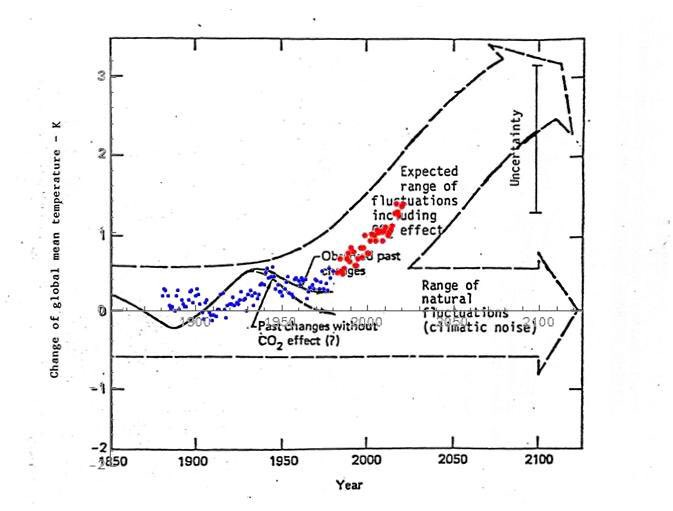
\includegraphics{fig/Exxon_Paths_Chart.jpeg}

After deepening the company's understanding of an environmental problem it suspected could harm its business, Exxon put its muscle behind efforts to manufacture doubt about the reality of global warming.
They deliberately created doubt when their internal research confirmed how serious a threat it was.

\href{https://insideclimatenews.org/news/24102019/exxon-scientists-climate-research-testify-congess-denial/}{Lavelle (2019) Former Exxon Scientists Tell Congress of Oil Giant's Climate Research Before Exxon Turned to Denial}

\hypertarget{co2-vs-temperature-causality}{%
\chapter{CO2 vs Temperature: Causality}\label{co2-vs-temperature-causality}}

\hypertarget{temperature-lags-co2-during-deglaciation}{%
\section{Temperature lags CO2 during deglaciation}\label{temperature-lags-co2-during-deglaciation}}

\emph{Shakun Abstract}

The covariation of carbon dioxide (CO 2 ) concentration and temperature
in Antarctic ice-core records suggests a close
link between CO 2 and climate during the Pleistocene ice ages.
The role and relative importance of CO 2 in producing these
climate changes remains unclear, however,
in part because the ice-core deuterium record reflects local rather than
global temperature.
Here we construct a record of global surface temperature from 80 proxy records and show that
temperature is correlated with and generally lags CO 2 during
the last (that is, the most recent) deglaciation.
Differences between the respective temperature changes of the Northern Hemisphere and
Southern Hemisphere parallel variations in the strength of
the Atlantic meridional overturning circulation recorded in marine sediments.
These observations, together with transient global climate model simulations,
support the conclusion that an antiphased hemispheric temperature response to
ocean circulation changes superimposed on globally in-phase warming driven by increasing
CO 2 concentrations
is an explanation for much of the temperature change at the end of the most recent ice age.

\emph{Shakun Memo}

Understanding the causes of the Pleistocene ice ages has been a
significant question in climate dynamics since they were discovered in
the mid-nineteenth century. The identification of orbital frequencies
in the marine \({}^{18}O/{}^{16}O\) record, a proxy for global ice volume, in the
1970s demonstrated that glacial cycles are ultimately paced by
astronomical forcing.
Initial measurements of air bubbles in Antarctic ice
cores in the 1980s revealed that greenhouse gas concentrations also
increased and decreased over the last glacial cycle, suggesting they
too may be part of the explanation. The ice-core record now extends
back 800,000 yr and shows that local Antarctic temperature was
strongly correlated with and seems to have slightly led changes in
\(CO_2\) concentration.

The implication of this relationship for understanding the role of
\(CO_2\) in glacial cycles, however, remains unclear.
For instance, proxy data have variously been interpreted to suggest
that \(CO_2\) was the primary driver of the ice ages, a more modest
feedback on warming or, perhaps, largely a consequence rather than
cause of past climate change.

Similarly, although climate models
generally require greenhouse gases to explain globalization of the
ice-age signal, they predict a wide range (one-third to two-thirds) in
the contribution of greenhouse gases to ice-age cooling, with
additional contributions from ice albedo and other effects

Global temperature reconstructions and transient model simulations
spanning the past century and millennium have been essential to
the attribution of recent climate change, and a similar strategy would
probably improve our understanding of glacial cycle dynamics.

Here we use a network of proxy temperature records that provide broad
spatial coverage to show that global temperature closely tracked the
increase in \(CO_2\) concentration over the last deglaciation, and that
variations in the Atlantic meridional overturning circulation
(AMOC) caused a seesawing of heat between the hemispheres,
supporting an early hypothesis that identified potentially important
roles for these mechanisms.
These findings, supported by transient
simulations with a coupled ocean--atmosphere general circulation
model, can explain the lag of \(CO_2\) behind Antarctic temperature in
the ice-core record and are consistent with an important role for \(CO_2\)
in driving global climate change over glacial cycles.

The onset of
deglaciation, which features about 0.3 \({}^\circ C\) of global warming before
the initial increase in \(CO_2\) ,17.5 kyr ago.
\(CO_2\) was not the cause of initial warming.

The overall correlation and phasing of global
temperature and the overall correlation and phasing of global
\(CO_2\) are consistent with \(CO_2\) being an important
driver of global warming during the deglaciation, with the centennial-
scale lag of temperature behind \(CO_2\) being consistent with the thermal
inertia of the climate system owing to ocean heat uptake and ice
melting

Although other mechanisms contributed to climate change during
the ice ages, climate models suggest that their impacts were regional
and thus cannot explain the global extent of temperature changes
documented by our stacked record alone.

The lead of Antarctic temperature over global temperature indicates
spatial variability in the pattern of deglacial warming.

Southern Hemisphere temperature probably leads \(CO_2\) ,
consistent with the Antarctic ice-core results,
Northern Hemisphere temperature lags \(CO_2\).

Seesawing of
heat between the hemispheres explains the contrast between the lead of
Antarctic temperature over \(CO_2\) and the lag of global (and Northern
Hemisphere) temperature behind \(CO_2\).

Our global temperature stack and transient modelling point to \(CO_2\)
as a key mechanism of global warming during the last deglaciation.
Furthermore, our results support an interhemispheric seesawing of
heat related to AMOC variability and suggest that these internal heat
redistributions explain the lead of Antarctic temperature over \(CO_2\)
while global temperature was in phase with or slightly lagged \(CO_2\).
Lastly, the global proxy database suggests that parts of the northern
mid to high latitudes were the first to warm after the LGM, which
could have initiated the reduction in the AMOC that may have
ultimately caused the increase in \(CO_2\) concentration.

\href{https://www.researchgate.net/publication/223987444_Global_Warming_Preceded_by_Increasing_Carbon_Dioxide_Concentrations_during_the_Last_Deglaciation}{Shakun (2012) Global Warming Preceded by Increasing Carbon Dioxide Concentrations during the Last Deglaciation}
\href{pdf/Shakun_2012_Warming_Preceded_by_CO2.pdf}{(pdf)}
\href{https://skepticalscience.com/skakun-co2-temp-lag.html}{Review in Skeptical Scientist}

\hypertarget{hen-or-egg-causality}{%
\section{Hen-Or-Egg Causality}\label{hen-or-egg-causality}}

\emph{Koutsoyiannis Abstract}

It is common knowledge that increasing \(CO_2\) concentration plays a major role in
enhancement of the greenhouse effect and contributes to global warming. The purpose of this
study is to complement the conventional and established theory, that increased \(CO_2\) concentration
due to human emissions causes an increase in temperature, by considering the reverse causality.
Since increased temperature causes an increase in \(CO_2\) concentration, the relationship of atmospheric
\(CO_2\) and temperature may qualify as belonging to the category of ``hen-or-egg'' problems, where it is
not always clear which of two interrelated events is the cause and which the effect. We examine the
relationship of global temperature and atmospheric carbon dioxide concentration in monthly time
steps, covering the time interval 1980--2019 during which reliable instrumental measurements are
available. While both causality directions exist, the results of our study support the hypothesis that
the dominant direction is T → \(CO_2\) . Changes in \(CO_2\) follow changes in T by about six months on
a monthly scale, or about one year on an annual scale. We attempt to interpret this mechanism by
involving biochemical reactions as at higher temperatures, soil respiration and, hence, \(CO_2\) emissions,
are increasing.

\emph{Koutsoyiannis Memo}

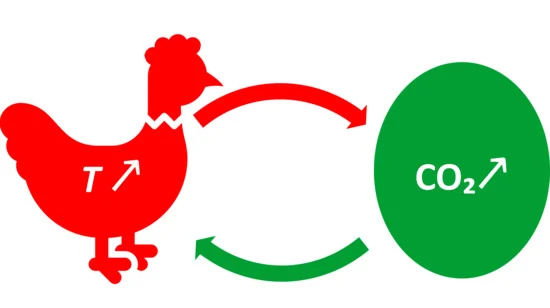
\includegraphics{fig/hen-or-egg.png}

We develop a stochastic framework, introducing useful notions of time irreversibility and system causality while we discuss the logical and technical complications in identifying causality, which prompt us to seek just necessary, rather than sufficient, causality conditions. In the Results section, we examine the relationship of these two quantities using the modern data, available at the monthly time step. We juxtapose time series of global temperature and atmospheric CO2 concentration from several sources, covering the common time interval 1980--2019. In our methodology, it is the timing rather than the magnitude of changes that is important, being the determinant of causality. While logical, physically based arguments support the ``hen-or-egg'' hypothesis, indicating that both causality directions exist, interpretation of cross-correlations of time series of global temperature and atmospheric CO2 suggests that the dominant direction is T → CO2, i.e., the change in temperature leads and the change in CO2 concentration follows. We attempt to interpret this latter mechanism by noting the positive feedback loop---higher temperatures increase soil respiration and, hence, CO2 emissions.

While we occasionally use the Granger statistical test, this is not central
in our approach.
Rather, we place the emphasis on time directionality in the relationship,
which we try to identify in the simplest possible manner, i.e.,
by \emph{finding the lag, positive or negative, which
maximizes the cross-correlation between the two processes.}

Another difference of our study, from most of the earlier ones, is our focus on changes, rather than
current states, in the processes we investigate. This puts the technique of process differencing in
central place in our analyses. This technique is quite natural and also powerful for studying time
directionality. We note that differencing has also been used in a study by Humlum et al.,
which has several similarities with our study, even though it is not posed in a formal causality context,
as well as in the study by Kodra et al.~However, differencing has been criticized for potentially
eliminating long-run effects and, hence, providing information only on short-run effects

\textbf{Data}

Our investigation of the relationship of temperature with concentration of carbon dioxide in
the atmosphere is based on two time series of the former process and four of the latter. Specifically,
the temperature data are of two origins, satellite and ground-based. The satellite dataset, developed
at the University of Alabama in Huntsville (UAH), infers the temperature, T, of three broad levels
of the atmosphere from satellite measurements of the oxygen radiance in the microwave band using
advanced (passive) microwave sounding units on NOAA and NASA satellites {[}47,48{]}. The data are
publicly available on the monthly scale in the forms of time series of ``anomalies'' (defined as differences
from long-term means) for several parts of earth as well as in maps. Here, we use only the global
average on monthly scale for the lowest level, referred to as the lower troposphere. The ground-based
data series we use is the CRUTEM.4.6.0.0 global T2m land temperature {[}49{]}. This originates from a
gridded dataset of historical near-surface air temperature anomalies over land. Data are available for
each month from January 1850 to the present. The dataset is a collaborative product of the Met Office Hadley Centre and the Climatic Research Unit at the University of East Anglia. We note that both
sources of information, UAH and CRUTEM, provide time series over the globe, land, and oceans; here,
we deliberately use one source for the globe and one for the land.

The two temperature series used in the study are depicted in Figure.

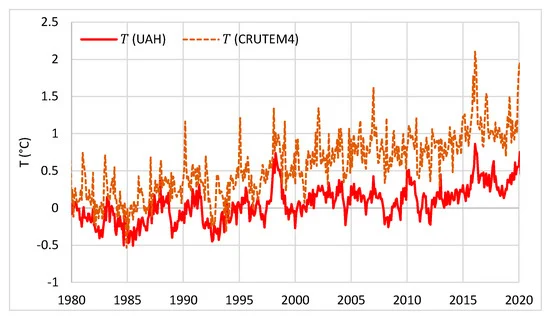
\includegraphics{fig/UAH_vs_CRUTEM4.png}

They are consistent with
each other (and correlated, r = 0.8), though the CRUTEM4 series shows a larger increasing trend than
the UAH series. The differences can be explained by three reasons: (a) the UAH series includes both
land and sea, while the chosen CRUTEM4 series is for land only, in which the increasing trend is
substantially higher than in sea; (b) the UAH series refers to some high altitude in the troposphere
(see details in Koutsoyiannis {[}50{]}), while the CRUTEM4 series refers to the ground level; and (c) the
ground-based CRUTEM4 series might be affected by urbanization (many ground stations are located
in urban areas). In any case, the difference in the increasing trends is irrelevant for the current study,
as the timing, rather than the magnitude, of changs is the determinant of causality.

\textbf{Methods}

\emph{Stochastic Framework}

A recent study {[}30{]} investigated time irreversibility in hydrometeorological processes and
developed a theoretical framework in stochastic terms. It also studied necessary conditions for
causality, which is tightly linked to time irreversibility.
A process that is not time-reversible is called time-asymmetric, time-irreversible, or time-directional.
Time asymmetry of a process can be studied more conveniently (or even exclusively in a scalar
process) through the differenced process.
To study irreversibility in vector processes, we can use second-order moments and, in particular,
cross-covariances among the different components of the vector.
Time (ir)reversibility could then be characterized by studying the properties of symmetry
or asymmetry of \(r_{x̃ ỹ}( ν, η )\) as a function of the time lag η.
Time asymmetry is closely related to causality, which presupposes irreversibility.
``No causal process (i.e., such that of two consecutive phases, one is always the cause of the other) can be reversible''
In probabilistic definitions of causality, time asymmetry is determinant.

Suppes {[}61{]} defines causation thus: ``An event \(B_{t'}\) {[}occurring at time t' {]}
is a prima facie cause of the event \(A_t\) {[}occurring at time t{]}
if and only if (i) t 0 \textless{} t, ( ii ) P\{\(B_{t'}\) \} \textgreater{} 0, (iii) P(\(A_t | B_{t'}\) ) \textgreater{} P(\(A_t\) )''.
In addition, Granger's {[}62{]} first axiom in defining causality reads,
``The past and present may cause the future, but the future cannot''.

Consequently, in simple causal systems, in which the process component \(x_τ\)
is the cause of \(y_τ\) (like in the clear case of rainfall and runoff, respectively),
it is reasonable to expect \(r_{x̃ỹ}[ ν, η ] ≥ 0\) for any η ≥ 0,
while \(r_{x̃ỹ}[ ν, η ] = 0\) for any η = 0.
However, in ``hen-or-egg'' causal systems, this will not be the case,
and we reasonably expect \(r_{x̃ỹ}[ ν, η ] != 0\) for any η.
Yet, we can define a dominant direction of causality
based on the time lag \(η_1\) maximizing cross-correlation.
Formally, \(η_1\) is defined for a specified ν as

\(η_1 : = argmax |r_{x̃ỹ} ( ν, η )|\) (over η)

We can thus distinguish the following three cases:

• If \(η_1 = 0\), then there is no dominant direction.

• If \(η_1 > 0\), then the dominant direction is \(x_τ → y_τ\) .

• If \(η_1 < 0\), then the dominant direction is \(y-τ_ → x_τ\) .

It must be stressed that the above conditions are considered as necessary and not sufficient
conditions for a causative relationship between the processes x τ and y . Following Koutsoyiannis {[}30{]}
τ
(where additional necessary conditions are discussed), we avoid seeking sufficient conditions, a task
that would be too difficult or impossible due to its deep philosophical complications as well as the
logical and technical ones.

In essence, the ``Granger causality test'' studies the improvement of prediction of a
process \(y_τ\) by considering the influence of a ``causing'' process \(x_τ\)

The rejection of the null hypothesis
is commonly interpreted in the literature with a statement that \(x_τ\) ``Granger-causes'' \(y_τ\).
This is clearly a misstatement and, in fact, the entire test is based on correlation matrices. Thus, it again reflects correlation rather than causation.
The rejection of the null hypothesis signifies improvement of prediction and
this does not mean causation.

Cohen {[}66{]} suggested replacing the term ``Granger causality'' with ``Granger prediction'' after
correctly pointing out this:

\begin{quote}
Results from Granger causality analyses neither establish nor require causality.
Granger causality results do not reveal causal interactions, although they can provide
evidence in support of a hypothesis about causal interactions.
\end{quote}

Some have thought they can approach genuine causes and get rid of the caution ``correlation is not
causation'' by replacing the correlation with other statistics in the mathematical description of causality.
For example, Liang {[}44{]} uses the concept of information (or entropy) flow (or transfer) between two
processes; this method has been called ``Liang causality'' in the already cited work he co-authors {[}43{]}.
The usefulness of such endeavours is not questioned, yet their vanity to determine genuine causality is
easy to infer: using any quantity
related to entropy (equivalently, information), is virtually identical to using correlation.
The information flow turns out to be the correlation coefficient multiplied by a constant.
In other words, the big philosophical
problem of causality cannot be resolved by technical tricks.
Thus, using any quantity related to entropy (equivalently, information),
is virtually identical to using correlation.

We assert that both causality directions exist, and we are looking for
the dominant one under the current climate conditions (those manifest in the datasets we use)
instead of trying to make assertions of an exclusive causality direction.

\emph{Conclusion}

In brief, all above confirm the results of our methodology that the dominant direction of causalityis T → \protect\hyperlink{co2}{CO2}.

\emph{Physical Interpretation}

The omnipresence of positive lags on both monthly and annual time scales and the confirmation
by Granger tests reduce the likelihood that our results are statistical artefacts. Still, our results require
physical interpretation which we seek in the natural process of soil respiration.
Soil respiration, R s , defined to be the flux of microbially and plant-respired CO 2 , clearly increases
with temperature. It is known to have increased in the recent years {[}74,75{]}. Observational data of R s
(e.g., {[}76,77{]}; see also {[}78{]}) show that the process intensity increases with temperature. Rate of chemical
reactions, metabolic rate, as well as microorganism activity, generally increase with temperature.
This has been known for more than 70 years (Pomeroy and Bowlus {[}79{]}) and is routinely used in
engineering design.
The Figure 6.1 of the latest report of the IPCC {[}75{]} provides a quantification of the mass balance
of the carbon cycle in the atmosphere that is representative of recent years. The soil respiration,
assumed to be the sum of respiration (plants) and decay (microbes), is 113.7 Gt C/year (IPCC gives
a value of 118.7 including fire, which along with biomass burning, is estimated to be 5 Gt C/year by
Green and Byrne {[}80{]}).
We can expect that sea respiration would also have increased. Moreover, outgassing from
the oceans must also have increased as the solubility of CO 2 in water decreases with increasing
temperature {[}14,81{]}. In addition, photosynthesis must have increased, as in the 21st century the Earth
has been greening, mostly due to CO 2 fertilization effects {[}82{]} and human land-use management {[}83{]}.
Specifically, satellite data show a net increase in leaf area of 2.3\% per decade {[}83{]}. The sums of carbon
outflows from the atmosphere (terrestrial and maritime photosynthesis as well as maritime absorption)
amount to 203 Gt C/year. The carbon inflows to the atmosphere amount to 207.4 Gt C/year and include
natural terrestrial processes (respiration, decay, fire, freshwater outgassing as well as volcanism and
weathering), natural maritime processes (respiration) as well as anthropogenic processes. The latter
comprise human CO 2 emissions related to fossil fuels and cement production as well as land-use
change, and amount to 7.7 and 1.1 Gt C/year, respectively. The change in carbon fluxes due to natural
processes is likely to exceed the change due to anthropogenic CO 2 emissions, even though the latter
are generally regarded as responsible for the imbalance of carbon in the atmosphere.

The results of the study support the hypothesis that both causality directions exist, with T → CO 2
being the dominant, despite the fact that CO 2 → T prevails in public, as well as in scientific, perception.
Indeed, our results show that changes in CO 2 follow changes in T by about six months on a monthly
scale, or about one year on an annual scale.
The opposite causality direction opens a nurturing interpretation question. We attempted to
interpret this mechanism by noting that the increase in soil respiration, reflecting the fact that the
intensity of biochemical process increases with temperature, leads to increasing natural CO 2 emission.
Thus, the synchrony of rising temperature and CO 2 creates a positive feedback loop.

\href{https://www.mdpi.com/2413-4155/2/4/83}{Koutsoyiannis (2020) Atmospheric Temperature and CO2 : Hen-Or-Egg Causality?}
\href{pdf/Koutsoyiannis_2020_Hen-Or-Egg_Causality.pdf}{(pdf)}

*Reviewer comments to Koutsoyannis (Connolly)**

On your proposed mechanism for T→CO2

In Section 6, you briefly postulate some of the mechanisms by which increasing T could cause increasing CO2.

I agree with you that increasing global temperatures should lead to increasing atmospheric CO2 from increased soil respiration. Indeed, in a recent paper - ÓhAiseadha et al.~(2020), we briefly pointed out that this leads to the surprising fact that the net night-time soil warming caused by wind farms is probably leading to an increase in biological CO2 emissions which may well be counteracting some (or all) of the reduction in anthropogenic CO2 emissions the wind farms are hoped to cause.

You might find some of the references we cite in Section 4.2.4 of ÓhAiseadha et al.~(2020) relevant for your arguments.

However, I would suggest that there are other mechanisms by which global temperatures could alter atmospheric CO2 concentrations -- and broadly they typically are of the same sign, i.e., more warming leading to increased atmospheric CO2 concentrations.

For instance, I would also note that the solubility of CO2 in water decreases with increasing temperature. So, it is plausible that increasing temperature could also cause increasing CO2 through outgassing from the oceans. This is something we are considering for a manuscript that we are working on. However, we are still evaluating this hypothesis, as we are realising there are several unresolved issues associated with the transfer of CO2 across the surface ocean/air boundary.

Nonetheless, the transfer of CO2 back and forth between the surface oceans and the atmosphere is an important component of the annual CO2 fluxes. Therefore, changes in average SST may also be contributing to changes in atmospheric CO2.

Also, we still haven't published this formally, but our current best explanation for the high seasonal variability of the Barrow (and other Arctic CO2 monitoring stations, e.g., Alert, Canada) is that it is probably related to the seasonality of sea ice. That is, when the oceans are covered by sea ice, no gaseous exchange can occur, but once the sea ice melts in the Arctic summer, CO2 can be exchanged. And because the sea surface temperature is relatively cold, the CO2 solubility is relatively high, i.e., CO2 enters the oceans.

If this hypothesis is correct, then it suggests that changes in average sea ice cover from changing global temperatures might also alter atmospheric CO2.

These proposed mechanisms are less well grounded in the literature than the soil respiration mechanism. However, I suggest that you should at least consider the possibility of other mechanisms.

\href{https://www.mdpi.com/2413-4155/2/4/77/review_report}{Connolly}

\hypertarget{causal-structure-by-information-flow-analysis}{%
\subsection{Causal Structure by Information Flow Analysis}\label{causal-structure-by-information-flow-analysis}}

\emph{Stips Abstract}

We use a newly developed technique that is based on
the information flow concept to investigate the
causal structure between the global radiative forcing and
the annual global mean surface temperature anomalies (GMTA) since 1850.
Our study unambiguously shows one-way causality between the total
Greenhouse Gases and GMTA.
Specifically, it is confirmed that the former, especially \(CO_2\) ,
are the main causal drivers of the recent warming.
A significant but smaller information flow comes from aerosol
direct and indirect forcing, and on short time periods, volcanic forcings.
In contrast the causality contribution from natural forcings (solar irradiance
and volcanic forcing) to the long term trend is not significant.
The spatial explicit analysis reveals that the anthropogenic forcing fingerprint
is significantly regionally varying in both hemispheres.
On paleoclimate time scales, however, the cause-effect direction is reversed:
temperature changes cause subsequent \(CO_2\) / \(CH_4\) changes.

\emph{Stips Memo}

In this study, we use a recently developed mathematical
method, which is capable of quantitatively evaluating the drive and feedback causal relation between time
series, to address the importance of the different forcing components on climate in a quantitative but model
independent way. This new method is based on the information flow (IF) concept.

The whole new formalism is derived from first principles,
rather than as an empirically defined ansatz,
with the property of causality guaranteed in proven theorems.
This is in contrast to other causality analyses, say that based on
Granger causality or convergent cross mapping (CCM).
The resulting formula is concise in form, involving only the common
statistics, namely sample covariances.
It also allows an explicit discrimination between correlation and causality:
causation implies correlation, but not vice versa
Causality is measured as the
time rate of information flowing from one time series to another.

A nonzero IF, or information transfer as it may appear in the literature,
from an event to another logically tells the strength of the
causality from the former to the latter, and a vanishing causality must entail a zero flow.
Transfer entropy and Granger causality, the two most extensively studied formalisms
of IF and causality analysis respectively, turn out to be equivalent up to a factor of 2.
In causality analysis, a principle (actually the only quantitatively stated fact)
that must be verified is that,
when the evolution of a dynamical event (say A) is independent of another (say B),
then the causality from B to A is nil.
It has long been found that Granger causality and transfer entropy
fail to verify this principle in many applications, giving rise to spurious causalities.

\textbf{Results}

We use this technique to analyse the recently measured global mean surface air
temperature anomalies (GMTA) and various reconstructed external forcings covering
the period from 1850 to 2005 (156 years).
To introduce the method we calculate the information flow (IF) in nat
(natural unit of information) per unit time {[}nat/ut{]}
from the 156 years annual time series of global \(CO_2\) concentration to GMTA
as 0.348 ± 0.112 nat/ut and − 0.006 ± 0.003 nat/ut in the reverse direction.
Obviously, the former is significantly different from zero, while the latter,
in comparison to the former, is negligible.
This result unambiguously shows a one-way causality in the sense that the
recent \(CO_2\) increase is causing the temperature increase, but not the other way around.

\textbf{Conclusions}

Using the IF concept we were able to confirm the inherent one-way causality between
human activities and global warming, as during the last 150 years the increasing
anthropogenic radiative forcing is driving the increasing global temperature,
a result that cannot be inferred from traditional time delayed correlation or
ordinary least square regression analysis.
Natural forcing (solar forcing and volcanic activities) contributes only marginally to
the global temperature dynamics during the last 150 years.
Human influence, especially via \(CO_2\) radiative forcing,
has been detected to be significant since about the 1960s.
This provides an independent statistical confirmation of
the results from process based modelling studies.

On very long time scales (800,000 years) the IF is only significant in
the direction from air temperature to \(CO_2\) .
This supports the idea that the feedback of GHGs to temperature changes
seems to be much slower than the fast response of
temperature to changes in GHGs.

The spatial explicit analysis strongly indicates that the increasing anthropogenic
forcing is causing very differing effects regionally with some regions in
the southern hemisphere showing large IF values.
Regions of significant IF do coincide with regions having stronger than average
recent warming trends.

\href{https://www.nature.com/articles/srep21691}{Stips (2016) On the causal structure between CO2 and global temperature}
\href{pdf/Stips_2016_Causal_structure_CO2_temperature.pdf}{(pdf)}

(See also rsts/Causation: Liang)

\hypertarget{the-1940s-co2-plateau}{%
\section{The 1940s CO2 Plateau}\label{the-1940s-co2-plateau}}

\emph{Bastos Abstract}

The high-resolution CO 2 record from Law Dome
ice core reveals that atmospheric CO 2 concentration stalled
during the 1940s (so-called CO 2 plateau). Since the fossil-
fuel emissions did not decrease during the period, this
stalling implies the persistence of a strong sink, perhaps sus-
tained for as long as a decade or more. Double-deconvolution
analyses have attributed this sink to the ocean, conceivably
as a response to the very strong El Niño event in 1940--
1942. However, this explanation is questionable, as recent
ocean CO 2 data indicate that the range of variability in the
ocean sink has been rather modest in recent decades, and
El Niño events have generally led to higher growth rates of
atmospheric CO 2 due to the offsetting terrestrial response.
Here, we use the most up-to-date information on the differ-
ent terms of the carbon budget: fossil-fuel emissions, four
estimates of land-use change (LUC) emissions, ocean uptake
from two different reconstructions, and the terrestrial sink
modelled by the TRENDY project to identify the most likely
causes of the 1940s plateau. We find that they greatly over-
estimate atmospheric CO 2 growth rate during the plateau pe-
riod, as well as in the 1960s, in spite of giving a plausible
explanation for most of the 20th century carbon budget, es-
pecially from 1970 onwards. The mismatch between recon-
structions and observations during the CO 2 plateau epoch of
1940--1950 ranges between 0.9 and 2.0 Pg C yr −1 , depend-
ing on the LUC dataset considered. This mismatch may be
explained by (i) decadal variability in the ocean carbon sink
not accounted for in the reconstructions we used, (ii) a further
terrestrial sink currently missing in the estimates by land-
surface models, or (iii) LUC processes not included in the
current datasets. Ocean carbon models from CMIP5 indi-
cate that natural variability in the ocean carbon sink could
explain an additional 0.5 Pg C yr −1 uptake, but it is unlikely
to be higher. The impact of the 1940--1942 El Niño on the
observed stabilization of atmospheric CO 2 cannot be con-
firmed nor discarded, as TRENDY models do not repro-
duce the expected concurrent strong decrease in terrestrial
uptake. Nevertheless, this would further increase the mis-
match between observed and modelled CO 2 growth rate dur-
ing the CO 2 plateau epoch. Tests performed using the OS-
CAR (v2.2) model indicate that changes in land use not cor-
rectly accounted for during the period (coinciding with dras-
tic socioeconomic changes during the Second World War)
could contribute to the additional sink required. Thus, the
previously proposed ocean hypothesis for the 1940s plateau
cannot be confirmed by independent data. Further efforts are
required to reduce uncertainty in the different terms of the
carbon budget during the first half of the 20th century and to
better understand the long-term variability of the ocean and
terrestrial CO 2 sinks.

\emph{Bastos Memo}

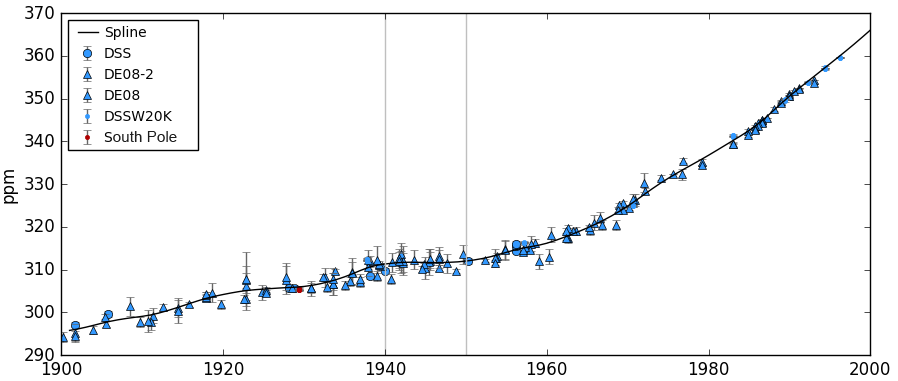
\includegraphics{fig/Law_Dome_CO2_1900-2000.png}

\emph{Figure: Atmospheric CO 2 concentration in the Law Dome ice
core and firn record from Rubino et al.~(2013) and respective un-
certainties (markers and whiskers) as well as the spline fit applied
to the data following Enting et al.~(2006), which attenuates by 50 \%
variations of ca. 23 years. The period corresponding to the plateau
is highlighted between vertical grey lines. The blue markers cor-
respond to samples from Law Dome and red markers from South
Pole; different symbols indicate the different ice cores (big mark-
ers) and firn samples (dots).}

Persistent El Niño sequences in
1895--1898 and 1911--1916 as well as the 1940s coincided
with small decreases in the CO 2 growth rate.

The very strong El Niño event that
lasted from 1940 until 1942 (Brönnimann et al., 2004) may
have been responsible for reduced upwelling of carbon-rich
waters in the Eastern Pacific, causing an abnormal increase
of the global ocean sink. However, this hypothesis remains
controversial and, moreover, in spite of the high quality of
the Law Dome δ 13 C record, the scatter and uncertainty in the
data are relatively high and they affect how well it is possible
to partition the biospheric and oceanic fluxes. Errors in the
δ 13 C data may lead to spurious and highly correlated terres-
trial and oceanic fluxes.

Rafelski et al.~(2009), using a single deconvolution of the
CO 2 record and a simple land-surface model, pointed to an
increased terrestrial sink during the 1940s. This sink was re-
lated to change in temperature. Single deconvolutions do not
use the δ 13 C information and assume time-invariant ocean re-
sponse. When terrestrial uptake is used to explain the 1940s
plateau they produce a peak in δ 13 C that appears to be incon-
sistent with the ice-core δ 13 C measurements, although the
differences are not large compared to the measurement un-
certainties.

Even if the unusually long 1940--1942 El
Niño did induce strong oceanic uptake, it is not clear that
it should have led to a decrease in CO 2 growth rate, as El
Niño periods in recent decades have usually been associ-
ated with a net increase in atmospheric CO 2 growth rate.
The occurrence of El Niño leads to reduced outgassing of CO 2 in the
tropical Pacific due to the slow-down of vertical upwelling
of carbon and nutrient-rich subsurface waters, driven by
weaker trade winds.

However, the magnitude of the El Niño/Southern Oscillation (ENSO) impact
on oceanic uptake differs significantly between studies, with
approaches based on \(δ^{13}\)C analysis pointing to anomalies of
1.5--2.5 Pg C yr −1 (Keeling et al., 1995; Joos et al., 1999;
Trudinger et al., 2002a), while atmospheric CO 2 -based meth-
ods point to anomalies of only 0.1--0.5 Pg C yr −1.

Furthermore, the enhancement of the global ocean sink during an El Niño event
is usually offset by a much larger terrestrial CO 2 release due
to the response of land ecosystems to widespread drought
conditions in the tropics and increased fire emissions.

Here, we evaluate whether it is possible to reproduce the
stabilization in atmospheric CO 2 during the 1940s using
model-based records of sources and sinks for the 20th cen-
tury and identify possible mechanisms to explain the plateau.
We first compare the atmospheric CO 2 growth rate recon-
structed using these datasets with the ice-core record to test
their ability to capture the plateau. Additionally, we evalu-
ate whether the ocean response to the 1940--1942 El Niño
may explain the atmospheric CO 2 stabilization. Finally, we
analyse the response of the land sink to this event using
land-surface process models and, given that land-use data are
highly uncertain, test the possible contribution of LUC to ex-
plain the additional sink required to match observations.

\emph{Bastos Conclusion}

Although the oceans are likely to
have contributed, they cannot by themselves provide the
complete explanation of the 1940s plateau. A strong terres-
trial sink is also required to match the observed stalling in
atmospheric CO 2 during the period.

In the case of the terrestrial sink, other
processes currently not included in the models or in the LUC
reconstructions may have contributed to the plateau. The ef-
fects of fire occurrence, changes in nutrient availability and
the devastating socioeconomic consequences of the Second
World War are examples of processes currently not well rep-
resented in the models.

\href{https://bg.copernicus.org/articles/13/4877/2016/}{Bastos (2016) Re-evaluating the 1940s CO2 plateau}
\href{pdf/Bastos_2016_Revealutaing_1940s_CO2_plateau.pdf}{(pdf)}

\hypertarget{origins-of-co2-increase}{%
\section{Origins of CO2 increase}\label{origins-of-co2-increase}}

\emph{Engelbeen}

In climate skeptics circles, there is rather much confusion about historical/present CO2 measurements. This is in part based on the fact that rather accurate historical direct measurements of CO2 in the atmosphere by chemical methods show much higher values in certain periods of time (especially around 1942), than the around 280 ppmv which is measured in Antarctic ice cores. 280 +/- 10 ppmv is assumed to be the pre-industrial amount of CO2 in the atmosphere during the current interglacial (the Holocene) by the scientific community. This is quite important, as if there were (much) higher levels of CO2 in the recent past, that may indicate that current CO2 levels are not from the use of fossil fuels, but a natural fluctuation and hence its influence on temperature is subject to (huge) natural fluctuations too and the current warmer climate is not caused by the use of fossil fuels.

To be sure about my skepticism: I like to see and examine the arguments of both sides of the fence, and I make up my own mind, based on these arguments. I am pretty sure that current climate models underestimate the role of the sun and other natural variations like ocean oscillations on climate and overestimate the role of greenhouse gases and aerosols. But I am as sure that the increase of CO2 in the atmosphere since the start of the industrial revolution is mainly from the use of fossil fuels.

\emph{Mass Balance}

The amount of CO2 emitted by humans nowadays is about 9 GtC/yr (CO2 counted as carbon). The increase in the atmosphere is about 5 GtC/yr.

In any year of the past over 50 years, the emissions are larger than the increase in the atmosphere. That means that the total mass balance of all natural variables (temperature, ocean pH, vegetation) which influence CO2 levels, is always towards more sink than source over any year.

The natural seasonal exchange between vegetation and oceans at one side and the atmosphere at the other side is estimated at about 150 GtC/yr. But that is not of interest for what the change is over a year, as most of the natural releases are absorbed within the same year. The difference after a year is not more than +/- 2 GtC, mainly caused by temperature changes (El Niño, Pinatubo eruption). Thus the natural variations over a year are smaller than the emissions. No matter how high the natural seasonal turnover might be, in all years over the previous near 50 years, the natural CO2 sinks were larger than the natural CO2 sources\ldots{} Thus it is near impossible that natural sources were responsible for (a substantial part of) the increase of CO2 in the past 50 years.

\emph{Isotopes}

Vegetation growth in general uses by preference 12C, thus if you measure δ13C in vegetation, you will see that it has quite low δ13C values. As almost all fossil fuels were formed from vegetation (or methanogenic bacteria, with similar preferences), these have low δ13C values too. Most other carbon sources (oceans, carbonate rock wearing, volcanic out gassing,\ldots) have higher δ13C values.

The δ13C levels as well as in the atmosphere as in the upper oceans start to decrease from 1850 on, that is at the start of the industrial revolution. In the 400 years before, there is only a small variation, probably caused by the temperature drop in the Little Ice Age. Longer term measurements of the δ13C ratio in CO2 from ice cores show that over the whole Holocene, the variations were not more than +/- 0.2 per mil. Even the change from a glacial to an interglacial period did not give more than 0.2 per mil δ13C change.

Again this is a good indication of the influence of fossil fuel burning\ldots{}

The 14C/12C ratio:

14C is a carbon isotope that is made in the atmosphere by the impact of cosmic rays. It is an unstable (radioactive) isotope and breaks down with a half-life time of about 6,000 years. 14C is used for radiocarbon dating of not too old fossils (maximum 60,000 years). The amount of 14C in the atmosphere is variable (depends of the sun's activity), but despite that, it allows to have a reasonable dating method. Until humans started to burn fossil fuels\ldots{}

The amounts of 14C in the atmosphere and in vegetation is more or less in equilibrium (as is the case for 13C: a slight depletion, due to 12C preference of the biological processes). But about halve of it returns to the atmosphere within a year, by the decay of leaves. Other parts need more time, but a lot is going back into the atmosphere within a few decades. For the oceans, the lag between 14C going into the oceans (at the North Atlantic sink place of the great conveyor belt) and its release around the equator is 500-1500 years, which gives a slight depletion of 14C, together with some very old carbonate going into solution which is completely 14C depleted. In pre-industrial times, there was an equilibrium between cosmogenic 14C production and oceanic depletion.

Fossil fuels at the moment of formation (either wood for coal or plankton for oil) incorporated some 14C, but as these are millions of years old, there is no measurable 14C anymore left. Just as is the case for 13C, the amount of CO2 released from fossil fuel burning diluted the 14C content of the atmosphere. This caused problems for carbon dating from about 1890 on. Therefore a correction table is used to correct samples of after 1890. In the 1950's another human intervention caused trouble for carbon dating: nuclear bomb testing induced a lot of radiation, which nearly doubled the atmospheric 14C content. Since then, the amount is fast reducing, as the oceans replace it with ``normal'' 14C levels. The half life time is about 14 years.

Again, this adds to the evidence that fossil fuel burning is the main cause of the increase of CO2 in the atmosphere\ldots{}

The ocean's pH and pCO2:

If oceanic CO2 (from the deep oceans to the surface and further into the atmosphere) was released, this should increase the 13C/12C ratio of both the upper oceans and the atmosphere, while we see the reverse. Moreover, the release of more CO2 from the upper oceans due to a lower pH would reduce the total amount of carbon (DIC: dissolved inorganic carbon, that is CO2 + bicarbonate + carbonate) in the ocean's surface layer. But we see the reverse trend: DIC is increasing over time {[}10{]}. Thus the increase of atmospheric CO2 is going into the oceans, not reverse.

There are huge differences in oceanic pCO2 at different latitudes due to changes in temperature and DIC. This gives a permanent release of CO2 in the tropics (pCO2 of maximum 750 µatm in the upper oceans vs.~about 400 µatm for the atmosphere) and a permanent sink of CO2 in the polar oceans, especially in the North-East Atlantic (minimum 150 µatm vs.~400 µatm). The oceans at mid-latitudes are seasonal emitters/absorbers of CO2, depending of the water temperature and sea life (plankton). The average yearly global difference of pCO2(atmosphere) - pCO2(oceans) is about 7 ppmv. That means that in average more CO2 is going from the atmosphere into the oceans than reverse {[}4{]}. Moreover, different surveys over time revealed that ocean parts which were net sources of CO2 gradually changed into net absorbers.

Although the ocean pCO2 data are scattered in time and covered area, the trends are clear that the average (increasing) flow of CO2 is from the atmosphere into the oceans and not reverse.

\emph{Engelbeen Conclusion}

From the available evidence it is quite clear that human emissions are the main cause of the increase of CO2 in the atmosphere. There is a small influence of temperature on this increase, as warmer oceans emit some CO2 (but warmer land absorbs more CO2 in vegetation!). The influence of temperature is limited: based on the variability of the CO2 increase around the trend, the short-term (seasons to 2-3 years) ratio is 4-5 ppmv/ºC (based on the seasonal and opposite temperature related 1992 Pinatubo and 1998 El Niño events). The very long term influence of temperature on CO2 levels (Vostok ice core) is about 8 ppmv/ºC. Thus at maximum, the influence of temperature on the current increase since the LIA is 0.8 ºC x 8 ppmv/ºC = 6.4 ppmv of the over 100 ppmv increase since the start of the industrial revolution.

There are only two fast main sources of CO2 to the atmosphere, besides the burning of fossil fuels: oceans and vegetation. Vegetation is not a source of CO2, as the oxygen deficiency (see chapter 1.5) showed. Neither are the oceans, as the δ13C trend (see chapter 1.3) and the pCO2/pH trends (see chapter 1.6) shows. This is more than sufficient to be sure that human emissions are the cause of most of the increase of CO2 in the atmosphere over the past 1.6 century.

Thus we may conclude:

All observed evidence from measurements all over the earth show with overwhelming evidence that humans are causing the bulk of the recent increase of CO2 into the atmosphere.

But\ldots{}

That humans are the cause of the recent increase of CO2 doesn't tell anything about the influence of increased CO2 on temperature!

\hypertarget{anthropogenic-co2}{%
\subsection{Anthropogenic CO2}\label{anthropogenic-co2}}

** Exchange Rates (turnover) vs Absorption Rates (sink capacity)**

From several discussions, I know that it is quite difficult to understand the two different mechanisms which govern the fate of human CO2 in the atmosphere: the fate of individual molecules, governed by exchange rates (``turnover'') and the fate of an increase in total CO2, governed by absorption rates (sink capacity).

Every year about 150 GtC of CO2 (somewhat less than 20\% of the total CO2 content) is exchanged between the atmosphere and the oceans/vegetation. That means that every single CO2 molecule from human or natural origin has a 20\% chance per year to be incorporated in vegetation or dissolved into the oceans.
This makes that the half life time (the ``residence'' time) of human CO2 in the atmosphere is only about 5 years.

Thus if humans emit 8 GtC in a given year, next year some 6.5 GtC is still of human origin, the rest was exchanged with CO2 from the oceans and vegetation. The second year, this still is 5.3 GtC, then 4.3 GtC, etc\ldots{} This is not completely accurate, as some of the ``human'' CO2 comes back next year(s), especially from vegetation, as much of vegetation is one-year old leaves, which rotting returns a high part of CO2 incorporated in previous years. This is less the case for the oceans, where more of the absorbed CO2 disappears into the deep oceans, where it isn't directly traceable anymore. There are techniques to follow human CO2 even there, where they use other recent human-made gases like CFC's and the extra 14CO2 spike from the atomic bomb tests 1945-1960 to track the past emissions. Anyway the ``half life'', that is the time period in which half of the human induced individual CO2 molecules disappears, is around 5 years.

Over longer periods, humans continue to emit (currently about 9 GtC/year) CO2. The accumulation over the last years thus is 9 + 7.2 + 5.8 + 4.6 + 3.7 +\ldots{} or about 40 GtC from the emissions over the past 30 years. That is only 5\% of the current atmosphere\ldots{}
Some conclude from this that humans are only responsible for 5\% of the CO2 increase and thus, as far as that influences temperature, also only for 5\% of the temperature increase. But that is a wrong assumption\ldots{}

The previous paragraphs are about how much human induced CO2 still is in the atmosphere. That is about the origin and fate of individual CO2 molecules, which atmospheric lifetime is governed by the seasonal turnover (back and forth flows) of about 150 GtC in/out the atmosphere from/to oceans and vegetation, and has nothing to do with the fate of the extra amount of CO2 (as mass) that humans emit, neither with the increase of total amount of CO2 in the atmosphere as result of that. The latter is governed by the net amounts which year by year are incorporated into oceans and vegetation. That is only 1-7 GtC/year (variable due to temperature variability) or in average 50-55\% of the emissions. The half life time of this extra CO2 (as mass) is much longer than the half life time of an individual CO2 molecule: around 40 years {[}14{]}. Thus if we should stop all CO2 emissions today, then the increase of 100 ppmv since the start of the industrial revolution would be reduced to 50 ppmv after some 40 years, further to 25 ppmv after 80 years and 12.5 ppmv after 120 years\ldots{}

\emph{Bern Model / Revell factor}

The IPCC comes with much longer half life times, according to the Bern model. This is a combination of relative fast (upper oceans), slower (deep oceans and more permanent storage in the biosphere) and very slow (rock weathering) sinks for the extra CO2. They assume that the first, relative fast, sinks of CO2 will reduce in capacity over the years. That is only true for the ocean surface layer, which follows the atmosphere quite rapidly (1-3 years), but is saturated at 10\% of the change in the atmosphere, due to the buffer/Revelle factor. Some media talk about hundreds to thousands of years that the extra CO2 will reside in the atmosphere. That is true for the last part of the curve, as the smaller amounts of CO2 are getting slower and slower into the sinks. But the bulk (87.5 \%) of the extra CO2 will disappear within 120 years as there is no sign of a slowdown of the sink capacity of the deep oceans and vegetation.

\href{http://www.ferdinand-engelbeen.be/klimaat/co2_origin.html}{Engelbeen (YYYY) ORIGIN OF THE RECENT CO2 INCREASE IN THE ATMOSPHERE}

\href{http://www.ferdinand-engelbeen.be/klimaat/co2_variability.html}{Engelbeeb (YYYY) ABOUT SPURIOUS CORRELATIONS AND CAUSATION OF THE CO2 INCREASE}

\emph{Stokes: Airborne Fraction (AF)}

The CO2 did start to rise while our emissions were small. I remarked that this is likely due to land clearance, which transfers C from the plant biomass to air.

The airborne fraction (AF) - the fraction of emission that stays in the air. I find that the added CO2 rises very linearly with total anthropogenic addition, and the AF is 44\%, with very little sign of change.

For the Mauna Loa period (1959-), the mass of C in the air plotted against all anthro addition (fossil + land use). It is very linear, and the regression slope is 0.439.

Airborne fraction is described in \href{https://www.ipcc.ch/publications_and_data/ar4/wg1/en/ch7s7-3-1-3.html\#7-3-2}{AR4 Ch 7}. It is often described in terms of AF of emissions, rather than total anthro.
The AF is of course larger, at 55\%, and is quite close to what Scripps quotes.

\href{https://moyhu.blogspot.com/2014/08/co2-accumulation-accounted-for-by.html}{Nick Stokes (Moyhu Blog 2014) CO2 accumulation accounted for by emission and land use}

\emph{Sealevel}

In paleoclimate reconstructions from ice cores, CO2 level changes generally lag temperature changes by hundreds of years, which is consistent with the fact that higher CO2 levels not only cause higher temperatures, but are also caused by higher ocean temperatures, and ocean temperature is slow to respond to air temperature changes.

Note that the rate at which the ocean absorbs CO2 from the air is proportional to CO2's partial pressure in the air. That's intuitively obvious when you remember that the concentration of CO2 in the air determines the rate at which CO2 molecules collide with and are absorbed by the surface of the ocean, and falling raindrops. So the measly 3\% per °C, by which CO2 solubility in water decreases as the water warms, is dwarfed by the 48\% by which solubility increased as atmospheric CO2 concentration rose by 48\% (from 280 ppmv to 414 ppmv), and as atmospheric CO2 level continues to rise, the rate at which the oceans remove CO2 from the air will continue to accelerate.

\href{https://sealevel.info/atmospheric_co2_increase_is_not_from_ocean_outgassing.html}{Sealevel.info}

\hypertarget{co2-isotopes}{%
\chapter{CO2 Isotopes}\label{co2-isotopes}}

\emph{NOAA}

Carbon-14 (or \({}^{14}C\)) is also known as radiocarbon, because it is the only carbon isotope that is radioactive. It is perhaps most famous for its use in radiocarbon dating of archeological artifacts ranging from mummies to cave drawings, and it plays a crucial role in studying fossil fuel carbon dioxide emissions as well.

Fossil fuels are, well, fossils, and are millions of years old. Because of this, all of the radiocarbon initially present has decayed away, leaving no \({}^{14}C\) in this ancient organic matter. All other atmospheric carbon dioxide comes from young sources--namely land-use changes (for example, cutting down a forest in order to create a farm) and exchange with the ocean and terrestrial biosphere. This makes \({}^{14}C\) an ideal tracer of carbon dioxide coming from the combustion of fossil fuels. Scientists can use \({}^{14}C\) measurements to determine how much \({}^{14}C\)O2 has been diluted with \({}^{14}C\)-free CO2 in air samples, and from this can calculate what proportion of the carbon dioxide in the sample comes from fossil fuels.

Unlike \({}^{14}C\), the amount of \({}^{13}C\) or \({}^{12}C\) in an artifact does not change over time since both \({}^{13}C\) and \({}^{12}C\) are stable isotopes. In other words, they do not decay. Because they are stable isotopes, a \({}^{13}C\) atom will always remain a \({}^{13}C\) atom, and the same is true for \({}^{12}C\).

Recall that there is much, much more \({}^{12}C\) than \({}^{13}C\) in the world --almost 99\% of all carbon atoms are \({}^{12}C\). Even so, different carbon pools have different ratios of \({}^{13}C\) and \({}^{12}C\) -- called isotopic fingerprints. The differences are small - one carbon pool may have 98.8\% \({}^{12}C\) while another may have 99.2\% \({}^{12}C\) - but modern machines, called isotope ratio mass spectrometers, can detect these differences quite easily. Pools with relatively more \({}^{13}C\) (less \({}^{12}C\)) are called ``heavy'' and those with less \({}^{13}C\) are called ``light''.

Let's look at the four main carbon pools with which climate scientists are concerned: the atmosphere, the terrestrial biosphere (land plants, animals, and soils), fossil fuels, and the ocean. The atmosphere has a certain ratio of \({}^{13}C\) to \({}^{12}C\). This ratio is affected by the isotopic fingerprint of the source of new carbon dioxide to the atmosphere. Some sources of carbon dioxide are ``heavy'' while others are ``light''. The ratio in the atmosphere is also affected by the isotopic fingerprint of carbon dioxide sinks. Do these sinks take in a lot of \({}^{13}C\) or very little relative to the amount of \({}^{12}C\) they take up from the atmosphere?

\hypertarget{suess-effect}{%
\section{Suess Effect}\label{suess-effect}}

So, we know that the ratio of carbon isotopes in atmospheric carbon dioxide samples is from a mixture of sources, and we also know the unique isotopic fingerprint of each of those sources. Using these two pieces of information, scientists can figure out why trends in Δ14C and δ13C occur. Globally, \emph{as atmospheric carbon dioxide levels continue to increase, both Δ14C and δ13C are decreasing over time}. This is called the Suess Effect -- named after Dr.~Suess who first discovered this phenomenon.

The steady downward trend in Δ14C of background air shows that the additional carbon dioxide added to the atmosphere must have a lower Δ14C value than what is already in the atmosphere. Well, we know that fossil fuels have a Δ14C signal of -1000‰, but that all other sources have a signal that is very close to that of ambient air (approximately + 45‰ in 2010, actually). Therefore, when CO2 from fossil fuels enter the atmosphere, the Δ14C value in the atmosphere goes down. We can precisely calculate how much the Δ14C value in the atmosphere goes down when fossil fuel CO2 is added. It turns out to be about a 3‰ decrease in Δ14C for every 1 ppm of fossil fuel CO2 added to the atmosphere.

\emph{Ocean}

When CO2 is released from the ocean to the atmosphere, it tends to have a Δ14C value slightly lower than the atmosphere, because some of the 14C in it has had time to decay. Over the oceans, and especially in the Southern Hemisphere (which is mostly ocean!) this is the most important effect on Δ14C.

\emph{Respiration}

However, over the land, there is another effect that we think about -- carbon released from plants and soils. Carbon dioxide taken up from the atmosphere by plants is eventually released back to the atmosphere by respiration, but only after a few years (typically 10-20 years). This means that a very small amount of the 14C has decayed away, and the Δ14C value of the CO2 from respiration (when organisms use energy and release carbon dioxide as a byproduct) is different than the atmosphere. Scientists have calculated exactly how much this changes Δ14C in the atmosphere, and it turns out to be not much -- to be sure though, when scientists use Δ14C measurements to calculate how much fossil fuel CO2 has been added to the atmosphere, they make a correction for this respiration effect.

\emph{Nuclear}
Nuclear power has a much higher Δ14C value than the atmosphere (which is what caused the 14C ``bomb spike'' in the 1960s).

\emph{13C}

The relative proportion of 13C in our atmosphere is steadily decreasing over time. Before the industrial revolution, δ13C of our atmosphere was approximately -6.5‰; now the value is around -8‰. Recall that plants have less 13C relative to the atmosphere (and therefore have a more negative δ13C value of around -25‰). Most fossil fuels, like oil and coal, which are ancient plant and animal material, have the same δ13C isotopic fingerprint as other plants. The annual trend--the overall decrease in atmospheric δ13C--is explained by the addition of carbon dioxide to the atmosphere that must come from the terrestrial biosphere and/or fossil fuels. In fact, we know from Δ14C measurements, inventories, and other sources, that this decrease is from fossil fuel emissions, and is an example of the Suess Effect.

\emph{Seasonal Variations}

Total atmospheric carbon dioxide levels (not isotopic ratios, but just total carbon dioxide) show strong seasonal variations. In the summer (in the northern hemisphere--where most of the Earth's land sits), carbon dioxide decreases as it is fixed by plants via photosynthesis. In the fall and winter, carbon dioxide increases as many plants stop photosynthesizing and some of the carbon dioxide they fixed is released through respiration from plants, animals, and soils. Seasonal δ13C variations show the opposite pattern. δ13C increases in the summer and decreases in the winter.

When plants take up carbon dioxide, they prefer 12C over 13C. This leaves relatively more 13C in the atmosphere, which increases the δ13C of the atmosphere. However, in the winter, when the plants release more carbon dioxide than they consume, this carbon dioxide entering the atmosphere is relatively poor in 13C. This decreases the δ13C of the atmosphere during the fall and winter of each year since the carbon dioxide released from the plants is relatively rich in 12C--decreasing the ratio of 13C to 12C in the atmosphere. (Northern Hemissphere).

\href{https://gml.noaa.gov/education/isotopes/c14tellsus.html}{NOAA}

\href{https://gml.noaa.gov/education/isotopes/stable.html}{NOAA Stable Carbon and thee Carbon Cycle}

\hypertarget{isotopic-discrimination-of-land-photosynthesis}{%
\section{Isotopic discrimination of land photosynthesis}\label{isotopic-discrimination-of-land-photosynthesis}}

\emph{Keeling Significance}

Climate change and rising CO2 are altering the behavior of land plants in ways that influence how much biomass they produce relative to how much water they need for growth. This study shows that it is possible to detect changes occurring in plants using long-term measurements of the isotopic composition of atmospheric CO2. These measurements imply that plants have globally increased their water use efficiency at the leaf level in proportion to the rise in atmospheric CO2 over the past few decades. While the full implications remain to be explored, the results help to quantify the extent to which the biosphere has become less constrained by water stress globally.

\emph{Keeling Abstract}

A decrease in the 13C/12C ratio of atmospheric CO2 has been documented by direct observations since 1978 and from ice core measurements since the industrial revolution. This decrease, known as the 13C-Suess effect, is driven primarily by the input of fossil fuel-derived CO2 but is also sensitive to land and ocean carbon cycling and uptake. Using updated records, we show that no plausible combination of sources and sinks of CO2 from fossil fuel, land, and oceans can explain the observed 13C-Suess effect unless an increase has occurred in the 13C/12C isotopic discrimination of land photosynthesis. A trend toward greater discrimination under higher CO2 levels is broadly consistent with tree ring studies over the past century, with field and chamber experiments, and with geological records of C3 plants at times of altered atmospheric CO2, but increasing discrimination has not previously been included in studies of long-term atmospheric 13C/12C measurements. We further show that the inferred discrimination increase of 0.014 ± 0.007‰ ppm−1 is largely explained by photorespiratory and mesophyll effects. This result implies that, at the global scale, land plants have regulated their stomatal conductance so as to allow the CO2 partial pressure within stomatal cavities and their intrinsic water use efficiency to increase in nearly constant proportion to the rise in atmospheric CO2 concentration.

\href{https://www.pnas.org/content/114/39/10361}{Keeling (2017) Atmospheric evidence for a global secular increase in carbon isotopic discrimination of land photosynthesis}

\hypertarget{isotopic-signature-of-anthropocene}{%
\section{Isotopic signature of Anthropocene}\label{isotopic-signature-of-anthropocene}}

\emph{Dean Abstract}

We consider whether the Anthropocene is recorded in the isotope geochemistry of the
atmosphere, sediments, plants and ice cores, and the time frame during which any changes are
recorded, presenting examples from the literature. Carbon and nitrogen isotope ratios have
become more depleted since the 19th century, with the rate of change accelerating after \textasciitilde{} ad
1950, linked to increased emissions from fossil fuel consumption and increased production of
fertiliser. Lead isotope ratios demonstrate human pollution histories several millennia into the
past, while sulphur isotopes can be used to trace the sources of acid rain. Radioisotopes have
been detectable across the planet since the 1950s because of atmospheric nuclear bomb tests and
can be used as a stratigraphic marker. We find there is isotopic evidence of widespread human
impact on the global environment, but different isotopes have registered changes at different
times and at different rates.

\href{pdf/Dean_2014_Isotopic_signature_of_Anthropocene.pdf}{Dean (2014) Is there an isotopic signature of the Anthropocene?(pdf)}

\hypertarget{decoupling}{%
\chapter{Decoupling}\label{decoupling}}

\emph{Hausfather}

\textbf{Absolute Decoupling of Economic Growth and Emissions in 32 Countries}

Between 1990 and 2019, global emissions of CO2 increased by 56\%. Historically, economic growth has been closely linked to increased energy consumption --- and increased CO2 emissions in particular --- leading some to argue that a more prosperous world is one that necessarily has more impacts on our natural environment and climate. There is a lively academic debate about our ability to ``absolutely decouple'' emissions and growth --- that is, the extent to which the adoption of clean energy technology can allow emissions to decline while economic growth continues.

Over the past 15 years, however, something has begun to change. Rather than a 21st century dominated by coal that energy modelers foresaw, global coal use peaked in 2013 and is now in structural decline.

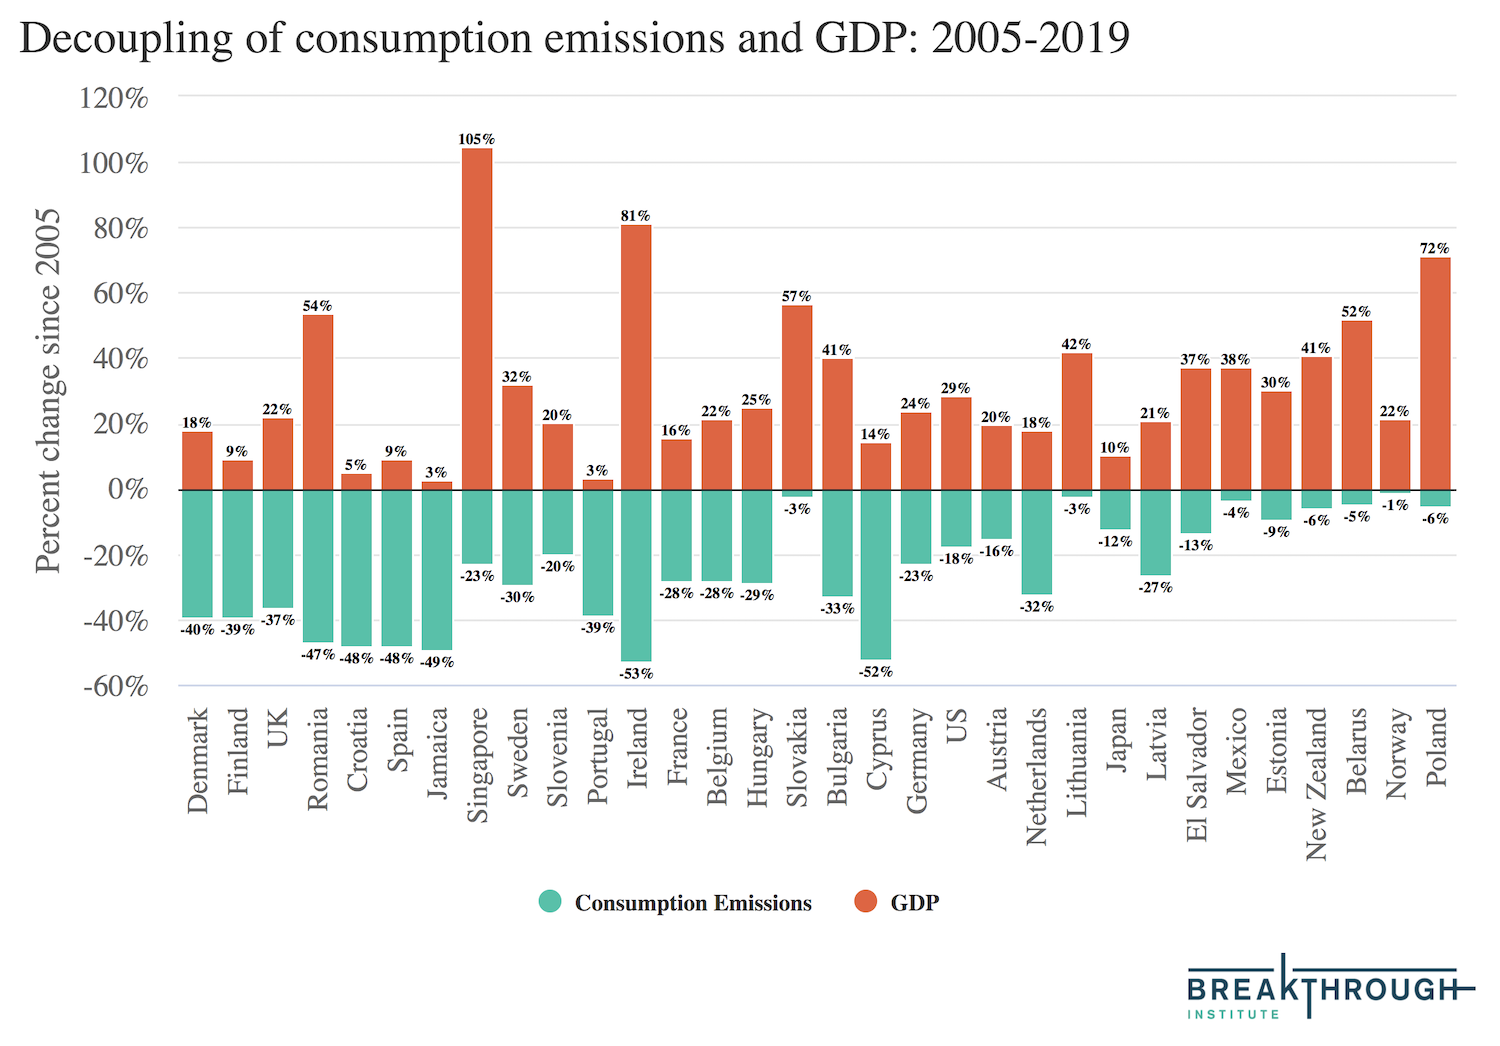
\includegraphics{fig/hausfather_decoupling.png}

These 32 countries show that it is possible to have economic growth at the same time that CO2 emissions decline, even accounting for embodied emissions in goods imported from overseas. However, these are mostly relatively wealthy countries whose economies tend to be increasingly driven by lower-energy information technology and service sectors. We have relatively few examples of low- or middle-income countries with a focus on energy-intensive manufacturing experiencing absolute decoupling to date.

Absolute decoupling is possible. There is no physical law requiring economic growth --- and broader increases in human wellbeing --- to necessarily be linked to CO2 emissions. All of the services that we rely on today that emit fossil fuels --- electricity, transportation, heating, food --- can in principle be replaced by near-zero carbon alternatives, though these are more mature in some sectors (electricity, transportation, buildings) than in others (industrial processes, agriculture).

\href{https://thebreakthrough.org/issues/energy/absolute-decoupling-of-economic-growth-and-emissions-in-32-countries}{Hausfather}

\emph{Hubacek Abstract}

Decoupling economic growth from resource use and emissions is a precondition to stay within planetary bound-
aries. A number of countries have achieved a reduction in their production-based emissions in the past decade.
However, the decline in PBE has often been achieved via outsourcing of emissions to other countries, which may
even lead to higher emissions globally. Therefore, a consumption-based perspective that accounts for a country's
emissions along global supply chains should also be employed when investigating progress in decoupling. Here
we investigate the progress countries made in reducing their production-based and consumption-based emissions
despite growth in gross domestic product (GDP). We found that 32 out of 116 countries (mainly developed ones)
achieved absolute decoupling between GDP and production-based emissions in recent years (2015--2018), and 23
countries achieved absolute decoupling between GDP and consumption-based emissions. 14 countries have de-
coupled GDP growth from both production- and consumption-based emissions. Even countries that have achieved
absolute decoupling are still adding emissions to the atmosphere thus showing the limits of `green growth' and
the growth paradigm. We also observed that decoupling can be temporary, and decoupled countries may switch
back to increasing emissions, which means that continuous efforts are needed to maintain decoupling. An analysis
of driving factors shows that whether a country can achieve decoupling mainly depends on reducing emission
intensity along domestic and import supply chains. This highlights the importance of decarbonizing supply chains
and international collaboration in controlling emissions.

\emph{Hubacek Conclusion}

The results show that 32 countries (mainly developed ones) have ab-
solute decoupling between GDP and production-based emissions in re-
cent years (2015--2018). However, the decline in PBE could have been
achieved via outsourcing of emissions to other countries. Our analy-
sis shows that only 23 countries achieved absolute decoupling between
GDP and consumption-based emissions. Another 67 countries (or 58\%)
have relatively decoupled, and 19 (or 16\%) coupled economic growth
with CBE. 6 countries were in an economic recession during the study
period. We also observed that decoupling can be temporary, and decou-
pled countries may switch back to increasing emissions, which means
that continuous efforts are needed to maintain decoupling. An analysis
of driving factors shows that whether a country can achieve decoupling
mainly depends on reducing emission intensity along domestic and im-
port supply chains. This highlights the importance of decarbonizing sup-
ply chains and international collaboration in controlling emissions.
While there have been some achievements in decarbonizing global
value chains these have been by far not sufficient as overall global emis-
sions have continued to rise. Even though some countries have achieved
absolute decoupling, they are still adding emissions to the atmosphere
thus showing the limits of `green growth' and the growth paradigm.
Even if all countries decouple in absolute terms, this might still not be
sufficient to avert dangerous climate change. Therfore, decoupling can
only serve as one of the indicators and steps toward fully decarbonizing
the economy and society.

\href{https://www.sciencedirect.com/science/article/pii/S2666792421000664?via\%3Dihub}{Hubacek (2021) Evidence of Decoupling}
\href{pdf/Hubacek_2021_Evidence_of_Decoupling.pdf}{(pdf)}

\hypertarget{paleoclimate}{%
\chapter{Paleoclimate}\label{paleoclimate}}

Earth's paleoclimate history provides guidance with a precision and reliability that climate
models cannot match. Ice cores were usually the paleoclimate data source of choice for those
scientists concerned about human-made climate change. That's understandable because ice
cores provide precise data on atmospheric composition as well as climate change.
However, ice cores cover only several hundred thousand years. That sounds like a long time, but
Earth was mostly in ice ages during that time. The ice cores encompass several interglacial
periods, but none of them were much warmer than our present global temperature.
(James Hansen: Sophies Planet Ch.40)

\hypertarget{holocen-thermal-maxima}{%
\section{Holocen Thermal Maxima}\label{holocen-thermal-maxima}}

\emph{Abstract Bova}

Proxy reconstructions from marine sediment cores indicate peak temperatures in the first half of the last and current interglacial periods (the thermal maxima of the Holocene epoch, 10,000 to 6,000 years ago, and the last interglacial period, 128,000 to 123,000 years ago) that arguably exceed modern warmth1,2,3. By contrast, climate models simulate monotonic warming throughout both periods4,5,6,7. This substantial model--data discrepancy undermines confidence in both proxy reconstructions and climate models, and inhibits a mechanistic understanding of recent climate change. Here we show that previous global reconstructions of temperature in the Holocene1,2,3 and the last interglacial period8 reflect the evolution of seasonal, rather than annual, temperatures and we develop a method of transforming them to mean annual temperatures. We further demonstrate that global mean annual sea surface temperatures have been steadily increasing since the start of the Holocene (about 12,000 years ago), first in response to retreating ice sheets (12 to 6.5 thousand years ago), and then as a result of rising greenhouse gas concentrations (0.25 ± 0.21 degrees Celsius over the past 6,500 years or so). However, mean annual temperatures during the last interglacial period were stable and warmer than estimates of temperatures during the Holocene, and we attribute this to the near-constant greenhouse gas levels and the reduced extent of ice sheets. We therefore argue that the climate of the Holocene differed from that of the last interglacial period in two ways: first, larger remnant glacial ice sheets acted to cool the early Holocene, and second, rising greenhouse gas levels in the late Holocene warmed the planet. Furthermore, our reconstructions demonstrate that the modern global temperature has exceeded annual levels over the past 12,000 years and probably approaches the warmth of the last interglacial period (128,000 to 115,000 years ago).

\href{https://www.nature.com/articles/s41586-020-03155-x}{Bova (2021) Nature (Paywall)}

\hypertarget{pattern-effect}{%
\chapter{Pattern Effect}\label{pattern-effect}}

\emph{Abtract}

Our planet's energy balance is sensitive to spatial inhomogeneities in sea surface temperature and sea ice changes, but this is typically ignored in climate projections. Here, we show the energy budget during recent decades can be closed by combining changes in effective radiative forcing, linear radiative damping and this pattern effect. The pattern effect is of comparable magnitude but opposite sign to Earth's net energy imbalance in the 2000s, indicating its importance when predicting the future climate on the basis of observations. After the pattern effect is accounted for, the best-estimate value of committed global warming at present-day forcing rises from 1.31 K (0.99--2.33 K, 5th--95th percentile) to over 2 K, and committed warming in 2100 with constant long-lived forcing increases from 1.32 K (0.94--2.03 K) to over 1.5 K, although the magnitude is sensitive to sea surface temperature dataset. Further constraints on the pattern effect are needed to reduce climate projection uncertainty.

\href{https://www.nature.com/articles/s41558-020-00955-x}{Nature article (paywall)}

\hypertarget{temperature-measurements}{%
\chapter{Temperature Measurements}\label{temperature-measurements}}

Temperatures have increased over virtually the entire planet since the mid-19th century, but the warming rate has not been the same everywhere.

When looking at the changes relative to the global average, it is clear the Arctic and land areas are warming faster than the ocean.

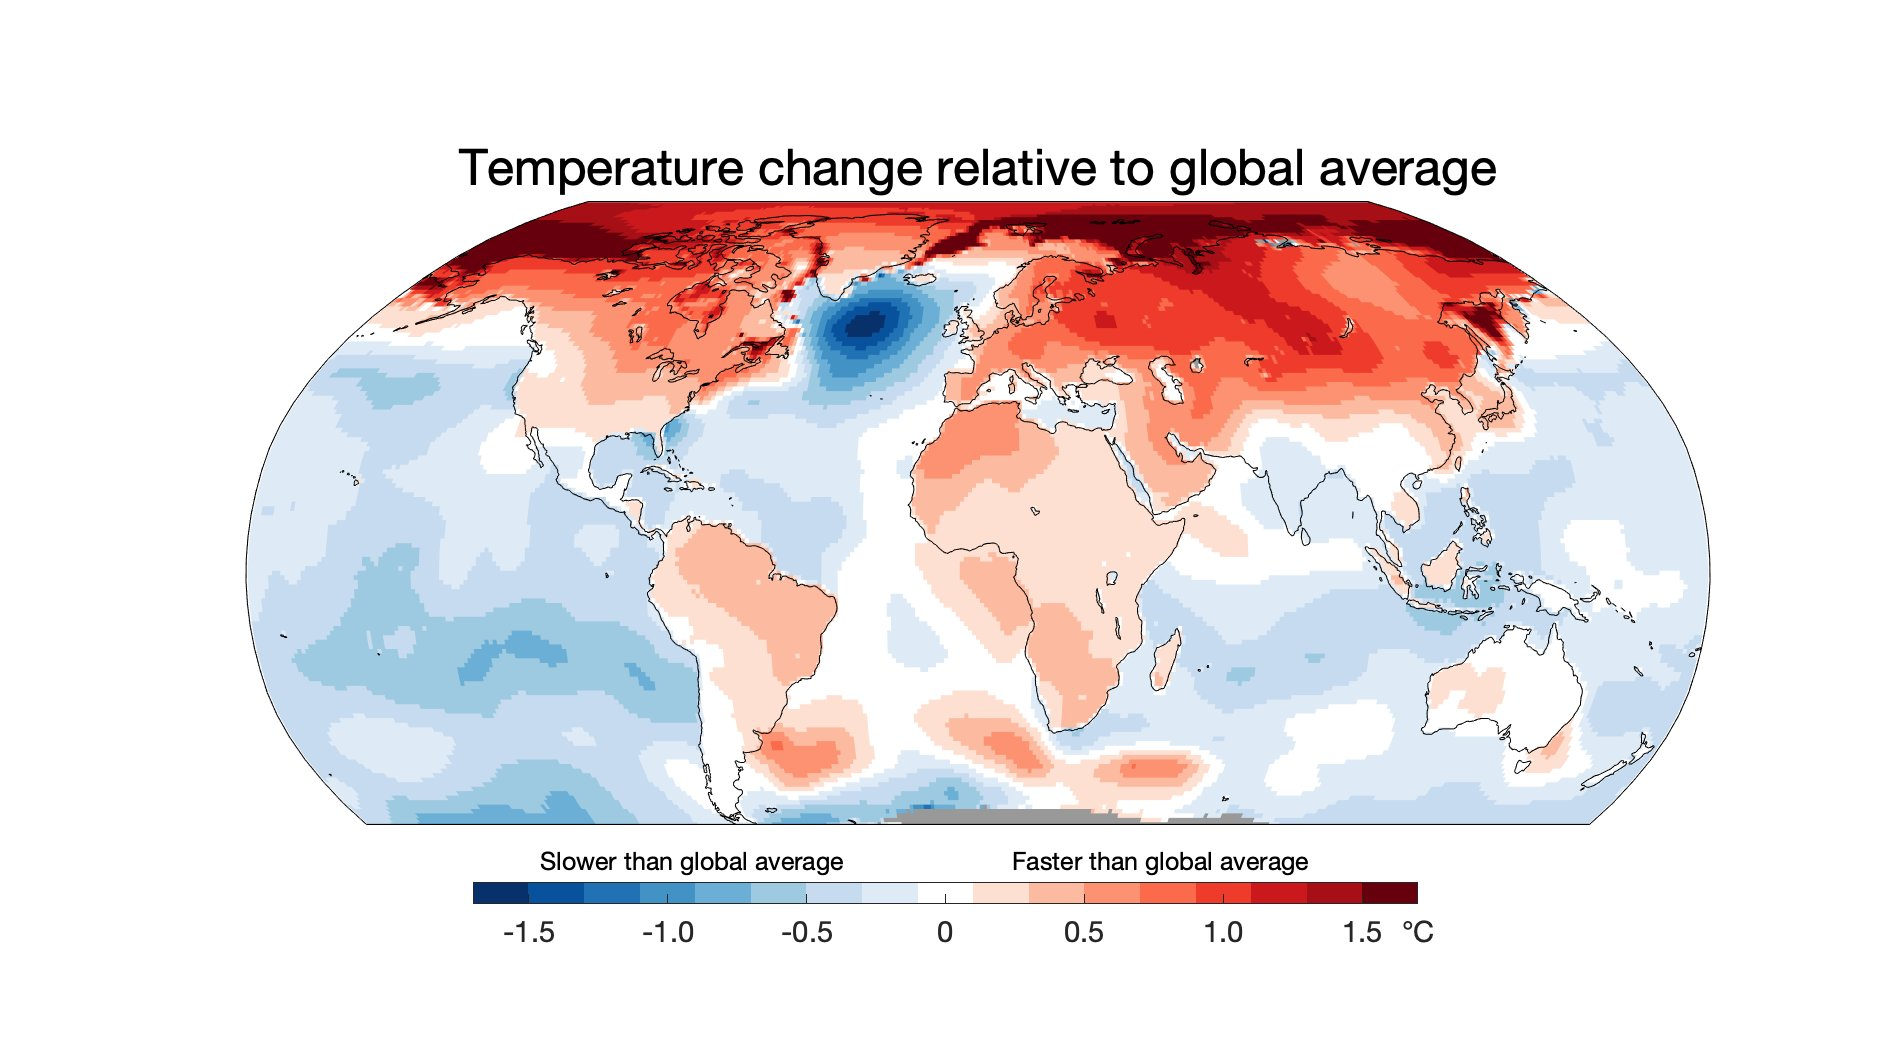
\includegraphics{fig/World_Temp_Change_Speed.jpeg}

\hypertarget{hockey-stick-graph}{%
\section{Hockey Stick Graph}\label{hockey-stick-graph}}

\href{https://en.wikipedia.org/wiki/Hockey_stick_graph}{Wikipedia}

\emph{Whal abstract}

The Mann et al.~(1998) Northern Hemisphere annual temperature reconstruction
over 1400--1980 is examined in light of recent criticisms concerning the nature and pro-
cessing of included climate proxy data. A systematic sequence of analyses is presented that
examine issues concerning the proxy evidence, utilizing both indirect analyses via exclusion
of proxies and processing steps subject to criticism, and direct analyses of principal compo-
nent (PC) processing methods in question. Altogether new reconstructions over 1400--1980
are developed in both the indirect and direct analyses, which demonstrate that the Mann et
al.~reconstruction is robust against the proxy-based criticisms addressed. In particular, re-
constructed hemispheric temperatures are demonstrated to be largely unaffected by the use
or non-use of PCs to summarize proxy evidence from the data-rich North American region.
When proxy PCs are employed, neither the time period used to ``center'' the data before PC
calculation nor the way the PC calculations are performed significantly affects the results,
as long as the full extent of the climate information actually in the proxy data is represented
by the PC time series. Clear convergence of the resulting climate reconstructions is a strong
indicator for achieving this criterion. Also, recent ``corrections'' to the Mann et al.~reconstruc-
tion that suggest 15th century temperatures could have been as high as those of the late-20th
century are shown to be without statistical and climatological merit. Our examination does
suggest that a slight modification to the original Mann et al.~reconstruction is justifiable for
the first half of the 15th century (∼ +0.05--0.10 ◦ ), which leaves entirely unaltered the primary
conclusion of Mann et al.~(as well as many other reconstructions) that both the 20th century
upward trend and high late-20th century hemispheric surface temperatures are anomalous.

\href{pdf/Wahl_2007_Robustness_of_Mann.pdf}{Whal (2007) Robustness of the Mann, Bradley, Hughes reconstruction (pdf)}

\hypertarget{water-vapor}{%
\chapter{Water Vapor}\label{water-vapor}}

\emph{SkepticalScience}

The amount of water vapor in the atmosphere exists in direct relation to the temperature. If you increase the temperature, more water evaporates and becomes vapor, and vice versa. So when something else causes a temperature increase (such as extra CO2 from fossil fuels), more water evaporates. Then, since water vapor is a greenhouse gas, this additional water vapor causes the temperature to go up even further---a positive feedback.

How much does water vapor amplify CO2 warming? Studies show that water vapor feedback roughly doubles the amount of warming caused by CO2. So if there is a 1°C change caused by CO2, the water vapor will cause the temperature to go up another 1°C. When other feedback loops are included, the total warming from a potential 1°C change caused by CO2 is, in reality, as much as 3°C.

The other factor to consider is that water is evaporated from the land and sea and falls as rain or snow all the time. Thus the amount held in the atmosphere as water vapour varies greatly in just hours and days as result of the prevailing weather in any location. So even though water vapour is the greatest greenhouse gas, it is relatively short-lived. On the other hand, CO2 is removed from the air by natural geological-scale processes and these take a long time to work. Consequently CO2 stays in our atmosphere for years and even centuries. A small additional amount has a much more long-term effect.

Generally it is held that the WV condenses out within a period of 14days.

As atmospheric CO2 levels rise relentlessly week on week, month on month, year on year, atmospheric water vapour reaches a rapid equilibration according to its vapour pressure in relation to the atmospheric presure and temperature.

Water vapour isn't 10x more effective a GC than CO2. Despite the fact that the water vapour concentration of the atmosphere is 5 times that of CO2 (around 0.3\% by mass for water vapour cf around 0.06\% by mass for CO2), the contribution of CO2 to the greenhouse effect is at least 10\% (and more like 25-30\% with the water vapour feedback).

Atmospheric CO2 doesn't fall out of the atmosphere. As we pump CO2 into the atmosphere it accumulates day by day, month by month, year by year. That can't happen with water vapor.

Atmospheric CO2 concentrations rise cumulatively (and very very quickly now).
The water vapour that we pump into the atmosphere is a tiny supplement to the natural evaporative/precipitation cycle, and since this comes straight out of the lower atmosphere within a week or two it can (a) have only a very small effect and (b) caanot be cumulative.

Man can't ``add'' water vapour to the atmosphere. The atmospheric water vapour levels are essentially ``defined'' by the atmospheric temperature and pressure.
What happens to all of that water (e.g the vast amount from natural evaporation)?. It all comes straight out as precipitation. What stays in the atmosphere is what the atmosphere can support in relation to the atmospheric temperature and pressure. In fact the research indicates that the atmosphere tends to maintain a relatively constant relative humidity.

\href{https://skepticalscience.com/water-vapor-greenhouse-gas.htm}{SkepticalScience}

\emph{ACS}

It's true that water vapor is the largest contributor to the Earth's greenhouse effect. On average, it probably accounts for about 60\% of the warming effect. However, water vapor does not control the Earth's temperature, but is instead controlled by the temperature. This is because the temperature of the surrounding atmosphere limits the maximum amount of water vapor the atmosphere can contain. If a volume of air contains its maximum amount of water vapor and the temperature is decreased, some of the water vapor will condense to form liquid water. This is why clouds form as warm air containing water vapor rises and cools at higher altitudes where the water condenses to the tiny droplets that make up clouds.

The greenhouse effect that has maintained the Earth's temperature at a level warm enough for human civilization to develop over the past several millennia is controlled by non-condensable gases, mainly carbon dioxide, CO2, with smaller contributions from methane, CH4, nitrous oxide, N2O, and ozone, O3. Since the middle of the 20th century, small amounts of man-made gases, mostly chlorine- and fluorine-containing solvents and refrigerants, have been added to the mix. Because these gases are not condensable at atmospheric temperatures and pressures, the atmosphere can pack in much more of these gases . Thus, CO2 (as well as CH4, N2O, and O3) has been building up in the atmosphere since the Industrial Revolution when we began burning large amounts of fossil fuel.

If there had been no increase in the amounts of non-condensable greenhouse gases, the amount of water vapor in the atmosphere would not have changed with all other variables remaining the same. The addition of the non-condensable gases causes the temperature to increase and this leads to an increase in water vapor that further increases the temperature. This is an example of a positive feedback effect. The warming due to increasing non-condensable gases causes more water vapor to enter the atmosphere, which adds to the effect of the non-condensables.

There is also a possibility that adding more water vapor to the atmosphere could produce a negative feedback effect. This could happen if more water vapor leads to more cloud formation. Clouds reflect sunlight and reduce the amount of energy that reaches the Earth's surface to warm it. If the amount of solar warming decreases, then the temperature of the Earth would decrease. In that case, the effect of adding more water vapor would be cooling rather than warming. But cloud cover does mean more condensed water in the atmosphere, making for a stronger greenhouse effect than non-condensed water vapor alone -- it is warmer on a cloudy winter day than on a clear one. Thus the possible positive and negative feedbacks associated with increased water vapor and cloud formation can cancel one another out and complicate matters. The actual balance between them is an active area of climate science research.

\href{https://www.acs.org/content/acs/en/climatescience/climatesciencenarratives/its-water-vapor-not-the-co2.html}{ACS}

\hypertarget{part-elements}{%
\part{Elements}\label{part-elements}}

\hypertarget{albedo}{%
\chapter{Albedo}\label{albedo}}

Some text on Albedo

\hypertarget{atmosphere}{%
\chapter{Atmosphere}\label{atmosphere}}

\begin{verbatim}
- Emissions
    - CO2
    - NO2   
    - Methane
    -
- Attributing Emissions
    - Norway's Responsibility
\end{verbatim}

\hypertarget{emissions}{%
\section{Emissions}\label{emissions}}

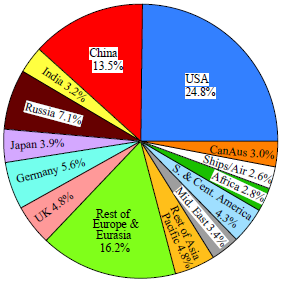
\includegraphics{fig/Emissions_Sum_1751-2018_by_Region.png}

Fig: Cumulative Emissions 1751-2018 by Country/Region

The UK (like the US) is 5X more responsible for global warming than the average nation.

\hypertarget{anual-greenhouse-gas-index-aggi}{%
\subsection{Anual Greenhouse Gas Index (AGGI)}\label{anual-greenhouse-gas-index-aggi}}

Figure shows radiative forcing for CO2, CH4, N2O and groupings of gases that capture changes predominantly in the CFCs, HCFCs, and the HFCs through 2021. Carbon dioxide is by far the largest contributor to total forcing from these gases and methane is the second largest contributor.

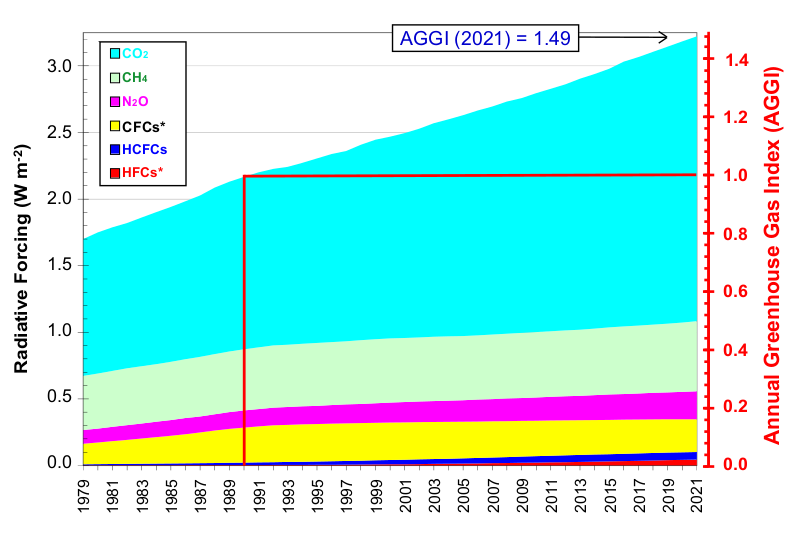
\includegraphics{fig/noaa_aggi.fig3.png}

\emph{Figure: Radiative forcing, relative to 1750, of virtually all long-lived greenhouse gases. The NOAA Annual Greenhouse Gas Index (AGGI), which is indexed to 1 for the year 1990, is shown on the right axis. The ``CFC\emph{'' grouping includes some other long-lived gases that are not CFCs (e.g., CCl4, CH3CCl3, and Halons), but the CFCs account for the majority (95\% in 2021) of this radiative forcing. The ``HCFC'' grouping includes the three most abundant of these chemicals (HCFC-22, HCFC-141b, and HCFC-142b). The ``HFC}'' grouping includes the most abundant HFCs (HFC-134a, HFC-23, HFC-125, HFC-143a, HFC-32, HFC-152a, HFC-227ea, and HFC-365mfc) and SF6 for completeness, although SF6 only accounted for a small fraction of the radiative forcing from this group in 2021 (13\%). }

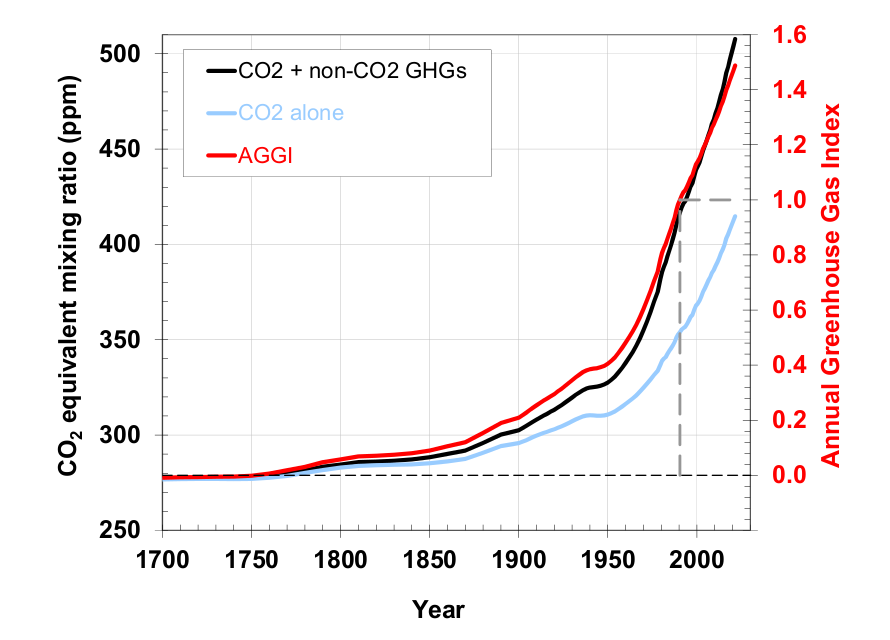
\includegraphics{fig/noaa_aggi.fig4.png}

\emph{Figure: Pre-1978 changes in the CO2-equivalent abundance and AGGI based on the ongoing measurements of all greenhouse gases reported here, measurements of CO2 going back to the 1950s from C.D. Keeling {[}Keeling et al., 1958{]}, and atmospheric changes derived from air trapped in ice and snow above glaciers {[}Machida et al., 1995, Battle et al., 1996, Etheridge, et al., 1996; Butler, et al., 1999{]}. Equivalent CO2 atmospheric amounts (in ppm) are derived with the relationship (Table 1) between CO2 concentrations and radiative forcing from all long-lived greenhouse gases. }

\href{https://gml.noaa.gov/aggi/aggi.html}{NOAA AGGI}

\hypertarget{co2}{%
\subsection{CO2}\label{co2}}

\emph{NOAA Global Monitoring Center}

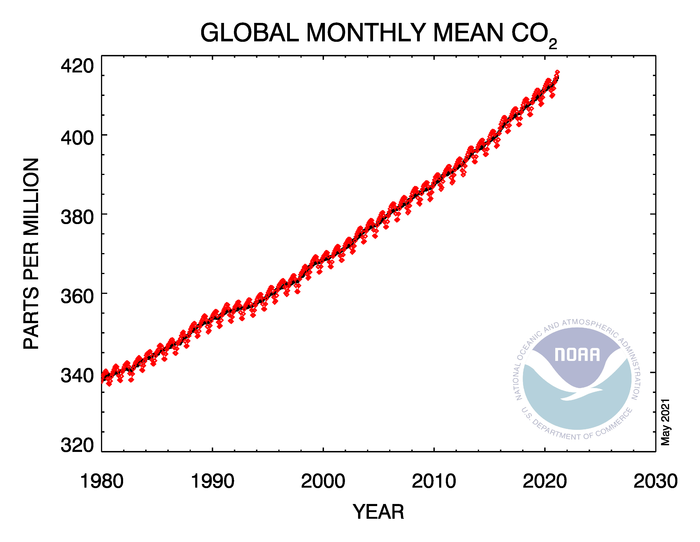
\includegraphics{fig/co2_trend_all_gl_may21.png}
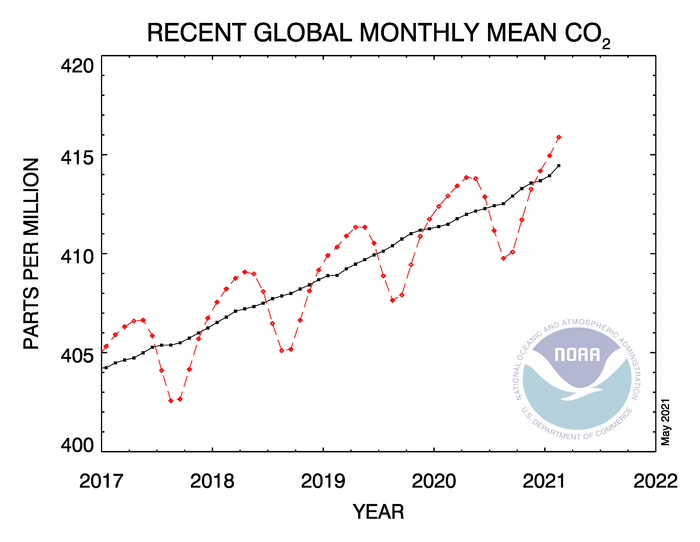
\includegraphics{fig/co2_trend_gl_may21.png}

\href{https://gml.noaa.gov/ccgg/trends/global.html}{NOAA Global Monitoring Center}

\emph{James Hansen}

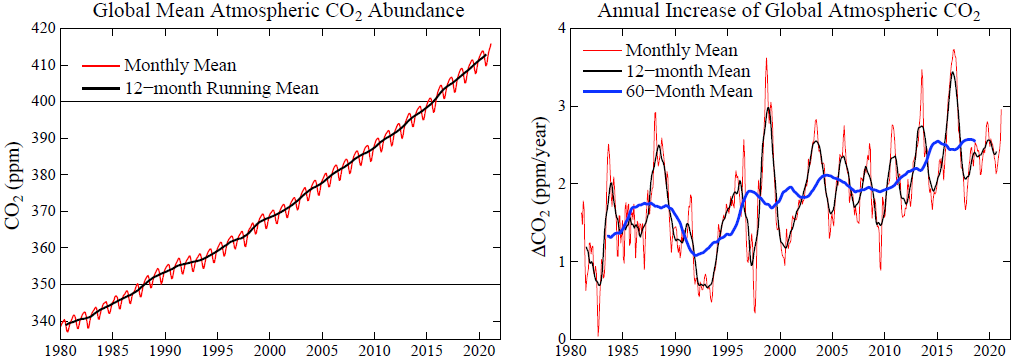
\includegraphics{fig/CO2_Annual_Increase.png}

The CO2 growth rate (Fig. 5) is now a bit below the peaks that occur in conjunction with strong El Ninos. However, the CO2 growth rate is not declining. CO2 growth has not even slowed as a result of the reduced economic activity associated with Covid-19.

\href{https://mailchi.mp/caa/the-world-has-cooled-off-whats-the-significance}{James Hansen 13 May 2021}

\hypertarget{measurement-of-co2}{%
\subsubsection{Measurement of CO2}\label{measurement-of-co2}}

\textbf{Mauna Loa}

\emph{Ryan Abstract}

A continuous 37 year record of the quiescent CO2 outgassing of Mauna Loa volcano was derived from atmospheric measurements made 6 km downslope of the summit caldera at Mauna Loa Observatory. The volcanic plume is sometimes trapped in the temperature inversion near the ground at night and transported downslope to the observatory. The amount of volcanic CO2 was greatest shortly after the 1975 and 1984 eruptions and then decreased exponentially with decay constants of 6.5 and 1.6 years respectively. Between 1959 and 1973 the decay constant was 6.1 years. The total reservoir mass of CO2 during each of the three quiescent periods was similar and estimated to be between 2 X 108 kg and 5 X 108 kg (0.2 Mt to 0.5 Mt). The 1975 eruption may have been preceded by a small increase in CO2 emissions. A similar increase has occurred since early 1993. Condensation nuclei (CN), presumably consisting of sulfate aerosol, were measured in the volcanic plume throughout the 1974 to 1994 record. The post-1975 period had consistently high levels of CN. Between 1977 and 1980, light-scattering aerosols were detected, coincident with a period of visible fuming at the summit. CN levels after the 1984 eruption were greatly reduced. Two brief periods of low CN emissions during this time correlate with temporary halts or reductions in the rate of summit expansion. These temporary reversals in the inflation of the mountain did not affect the steady exponential decline of the CO2 emissions rate. Upper limits were set on the amounts of H2O, O3, CH4, SO2, aerosol carbon, radon, CO, and H2 present in the plume at various periods between 1974 and 1993. The ratio of SO2 to CO2 was less than 1.8 X 10-3 between 1988 and 1992.

\href{https://web.archive.org/web/19980114152259/http://mloserv.mlo.hawaii.gov/publish/steve/VolcCO2.htm}{Ryan (1995) Quiescent Outgassing of Mauna Loa Volcano 1958-1994}

\href{https://gml.noaa.gov/obop/mlo/}{NOAA Mauna Loa Observatory}
\href{https://gml.noaa.gov/ccgg/about/co2_measurements.html}{dto. Measurement Methods}

\textbf{Wet Chemical Analysis}

\emph{Beck Abstract}

More than 90,000 accurate chemical analyses of CO2 in air since 1812 are summarised. The historic chemical data reveal that changes in CO2 track changes in temperature, and therefore climate in contrast to the simple, monotonically increasing CO2 trend depicted in the post-1990 literature on climate-change. Since 1812, the CO2 concentration in northern hemispheric air has fluctuated exhibiting three high level maxima around 1825, 1857 and 1942 the latter showing more than 400 ppm.

Between 1857 and 1958, the Pettenkofer process was the standard analytical method for determining atmospheric carbon dioxide levels, and usually achieved an accuracy better than 3\%. These determinations were made by several scientists of Nobel Prize level distinction. Following Callendar (1938), modern climatologists have generally ignored the historic determinations of CO2, despite the techniques being standard text book procedures in several different disciplines. Chemical methods were discredited as unreliable choosing only few which fit the assumption of a climate CO2 connection.

\href{https://journals.sagepub.com/doi/10.1260/095830507780682147}{Beck (2007) ``180 years of CO2 analysis by chemical methods'' (paywall)}

\href{pdf/Beck_CO2_Chemical.pdf}{Beck (pdf)}

\emph{Keeling on Beck}

Beck questions whether the rise in atmospheric CO2 over the past 50 years
is truly unprecedented, citing observations that appear to indicate much
higher variability inj the 19th and 20th centuries.
If Beck's contentions were true, they would overthrow 50 years of scientific advance
and discovery.
Unfortunately for Beck - as well as for humanity - yhe claim's don't stand up.

As Keeling grasped already in 1957 - before ha had shown that CO2 was increasing -
the earlier chemical measurements exhibit far too much geographic and short-term variability to plausibly be reprenstaive of the background.
The variablility of these early measurements must therefore be attributed to ``local or regional'' factors or poor measurement practice.

\href{https://www.jstor.org/stable/44397310?seq=1}{Keeling on Beck ``180 years of CO2 analysis by chemical methods''}

\hypertarget{antropogenic-co2}{%
\subsubsection{Antropogenic CO2}\label{antropogenic-co2}}

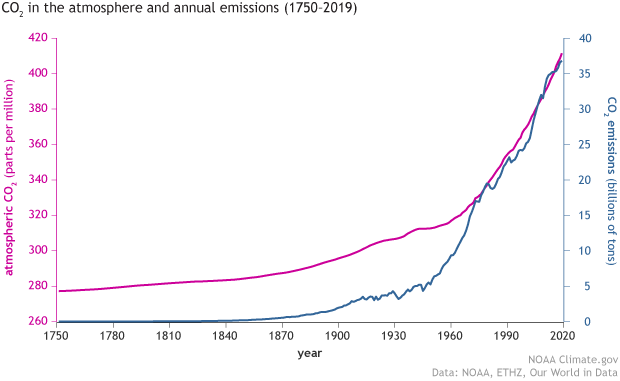
\includegraphics{fig/CO2_emissions_vs_concentrations_1751-2019.png}

\href{https://www.climate.gov/news-features/understanding-climate/climate-change-atmospheric-carbon-dioxide}{Figure Source}

\textbf{How do we know that recent CO2 increases are due to human activities?}

\href{https://www.realclimate.org/index.php/archives/2004/12/how-do-we-know-that-recent-cosub2sub-increases-are-due-to-human-activities-updated/}{RealClimate}

\href{https://www.realclimate.org/index.php/archives/2005/06/how-much-of-the-recent-cosub2sub-increase-is-due-to-human-activities/}{RealClimate Simple Explanation}

\href{https://www.realclimate.org/index.php/archives/2004/12/how-do-we-know-that-recent-co2-increases-are-due-to-human-activities/}{realClimate Technical}

\href{https://gml.noaa.gov/ccgg/isotopes/mixing.html}{NOAA Isotopes Measurement}

\emph{O'Connor}

Abstract: In this work, a semi-empirical relationship of carbon dioxide emissions with atmospheric
CO 2 concentrations has been developed that is capable of closely replicating observations from 1751
to 2018. The analysis was completed using data from fossil-fuel-based and land-use change based
CO 2 emissions, both singly and together. Evaluation of emissions data from 1750 to 1890 yields a
linear CO 2 concentration component that may be attributed to the net flux from land-use changes
combined with a rapidly varying component of the terrestrial sink. This linear component is then
coupled across the full-time period with a CO 2 concentration calculation using fossil-fuel
combustion/cement production emissions with a single, fixed fossil-fuel combustion airborne
fraction {[}AF FF {]} value that is determined by the ocean sink coupled with the remaining slowly
varying component of the land sink. The analysis of the data shows that AF FF has remained constant
at 51.3\% over the past 268 years. However, considering the broad range of variables including
emission and sink processes influencing the climate, it may not be expected that a single value for
AF FF would accurately reproduce the measured changes in CO 2 concentrations during the industrial
era.

\href{https://www.researchgate.net/publication/341129655_Modeling_of_Atmospheric_Carbon_Dioxide_CO2_Concentrations_as_a_Function_of_Fossil-Fuel_and_Land-Use_Change_CO2_Emissions_Coupled_with_Oceanic_and_Terrestrial_Sequestration}{O'Connor (2020) Modeling of Atmospheric Carbon Dioxide (CO2) Concentrations as a Function of Fossil-Fuel and Land-Use Change CO2 Emissions Coupled with Oceanic and Terrestrial Sequestration}
\href{pdf/OConner_2020_Fossil_CO2_Measurement.pdf}{(pdf)}
\href{pdf/OConner_2020_Fossil_CO2_Measurement_SI.pdf}{(pdf SI)}

\hypertarget{c14-measurement}{%
\subsubsection{C14 Measurement}\label{c14-measurement}}

\emph{Basu}

We report national scale estimates of CO2 emissions from fossil-fuel combustion and cement production in the United States based directly on atmospheric observations, using a dual-tracer inverse modeling framework and CO2 and Δ14CO2 measurements obtained primarily from the North American portion of the National Oceanic and Atmospheric Administration's Global Greenhouse Gas Reference Network. The derived US national total for 2010 is 1,653 ± 30 TgC yr−1 with an uncertainty (1σ) that takes into account random errors associated with atmospheric transport, atmospheric measurements, and specified prior CO2 and 14C fluxes. The atmosphere-derived estimate is significantly larger (\textgreater3σ) than US national emissions for 2010 from three global inventories widely used for CO2 accounting, even after adjustments for emissions that might be sensed by the atmospheric network, but which are not included in inventory totals. It is also larger (\textgreater2σ) than a similarly adjusted total from the US Environmental Protection Agency (EPA), but overlaps EPA's reported upper 95\% confidence limit. In contrast, the atmosphere-derived estimate is within 1σ of the adjusted 2010 annual total and nine of 12 adjusted monthly totals aggregated from the latest version of the high-resolution, US-specific ``Vulcan'' emission data product. Derived emissions appear to be robust to a range of assumed prior emissions and other parameters of the inversion framework. While we cannot rule out a possible bias from assumed prior Net Ecosystem Exchange over North America, we show that this can be overcome with additional Δ14CO2 measurements. These results indicate the strong potential for quantification of US emissions and their multiyear trends from atmospheric observations.

\href{https://www.pnas.org/content/117/24/13300}{Basu (2020) Estimating US fossil fuel CO2 emissions from measurements of C14 in atmospheric CO2}

\hypertarget{globale-co2-rise}{%
\subsubsection{Globale CO2 Rise}\label{globale-co2-rise}}

\textbf{The global CO2 rise: Facts and Denial Tricks}

\href{https://www.realclimate.org/index.php/archives/2018/01/the-global-co2-rise-the-facts-exxon-and-the-favorite-denial-tricks/}{RealClimate}

\hypertarget{turnover-time}{%
\subsubsection{Turnover time}\label{turnover-time}}

\textbf{Climate Myth: CO2 has a short residence time}

``{[}T{]}he overwhelming majority of peer-reviewed studies {[}find{]} that CO2 in the atmosphere remained there a short time.''

The claim goes like this:

\begin{quote}
\begin{enumerate}
\def\labelenumi{(\Alph{enumi})}
\tightlist
\item
  Predictions for the Global Warming Potential (GWP) by the IPCC express the warming effect CO2 has over several time scales; 20, 100 and 500 years.\\
\item
  But CO2 has only a 5 year life time in the atmosphere.\\
\item
  Therefore CO2 cannot cause the long term warming predicted by the IPCC.
\end{enumerate}
\end{quote}

This claim is false. (A) is true. (B) is also true. But B is irrelevant and misleading so it does not follow that C is therefore true.

The claim hinges on what life time means. To understand this, we have to first understand what a box model is: In an environmental context, systems are often described by simplified box models. A simple example (from school days) of the water cycle would have just 3 boxes: clouds, rivers, and the ocean.

A representation of the carbon cycle (ignore the numbers for now) would look like this one from NASA.

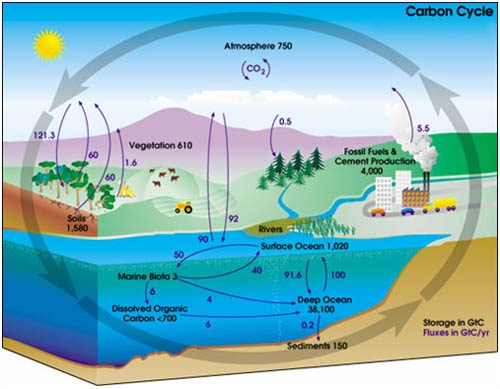
\includegraphics{fig/carbon_cycle_NASA.jpg}

In the IPCC 4th Assessment Report glossary, ``lifetime'' has several related meanings. The most relevant one is:

\begin{quote}
``Turnover time (T) (also called global atmospheric lifetime) is the ratio of the mass M of a reservoir (e.g., a gaseous compound in the atmosphere) and the total rate of removal S from the reservoir: T = M / S. For each removal process, separate turnover times can be defined. In soil carbon biology, this is referred to as Mean Residence Time.''
\end{quote}

In other words, life time is the average time an individual particle spends in a given box. It is calculated as the size of box (reservoir) divided by the overall rate of flow into (or out of) a box. The IPCC Third Assessment Report 4.1.4 gives more details.

In the carbon cycle diagram above, there are two sets of numbers. The black numbers are the size, in gigatonnes of carbon (GtC), of the box. The purple numbers are the fluxes (or rate of flow) to and from a box in gigatonnes of carbon per year (Gt/y).

A little quick counting shows that about 200 Gt C leaves and enters the atmosphere each year. As a first approximation then, given the reservoir size of 750 Gt, we can work out that the residence time of a given molecule of CO2 is 750 Gt C / 200 Gt C y-1 = about 3-4 years. (However, careful counting up of the sources (supply) and sinks (removal) shows that there is a net imbalance; carbon in the atmosphere is increasing by about 3.3 Gt per year).

It is true that an individual molecule of CO2 has a short residence time in the atmosphere. However, in most cases when a molecule of CO2 leaves the atmosphere it is simply swapping places with one in the ocean. Thus, the warming potential of CO2 has very little to do with the residence time of CO2.

What really governs the warming potential is how long the extra CO2 remains in the atmosphere. CO2 is essentially chemically inert in the atmosphere and is only removed by biological uptake and by dissolving into the ocean. Biological uptake (with the exception of fossil fuel formation) is carbon neutral: Every tree that grows will eventually die and decompose, thereby releasing CO2. (Yes, there are maybe some gains to be made from reforestation but they are probably minor compared to fossil fuel releases).

Dissolution of CO2 into the oceans is fast but the problem is that the top of the ocean is ``getting full'' and the bottleneck is thus the transfer of carbon from surface waters to the deep ocean. This transfer largely occurs by the slow ocean basin circulation and turn over (*3). This turnover takes 500-1000ish years. Therefore a time scale for CO2 warming potential out as far as 500 years is entirely reasonable (See IPCC 4th Assessment Report Section 2.10).

\href{https://skepticalscience.com/argument.php?p=3\&t=154\&\&a=80}{SkepticalScience}

\hypertarget{carbon-cycle}{%
\subsection{Carbon Cycle}\label{carbon-cycle}}

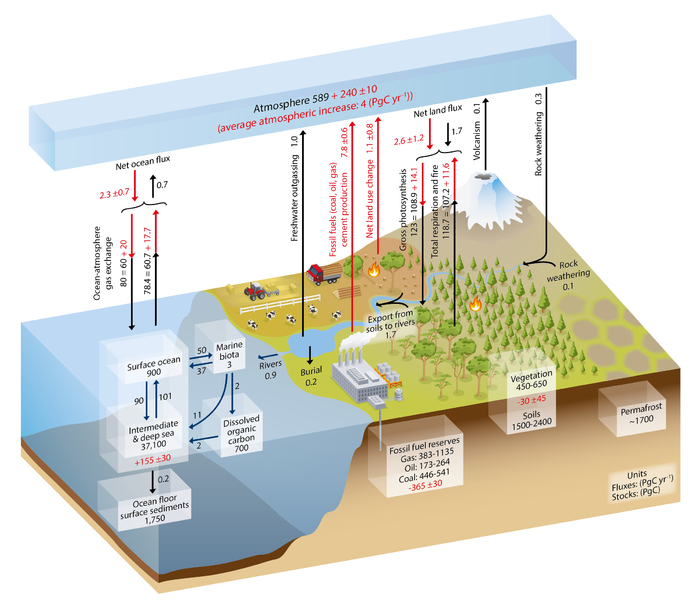
\includegraphics{fig/carbon_cycle_WG1AR5ch6.jpg}

\emph{Figure: Simplified schematic of the global carbon cycle. Numbers represent reservoir mass, also called `carbon stocks' in PgC (1 PgC = 10 15 gC) and annual carbon exchange
fluxes (in PgC yr --1 ). Black numbers and arrows indicate reservoir mass and exchange fluxes estimated for the time prior to the Industrial Era, about 1750 (see Section 6.1.1.1 for
references). Fossil fuel reserves are from GEA (2006) and are consistent with numbers used by IPCC WGIII for future scenarios. The sediment storage is a sum of 150 PgC of the
organic carbon in the mixed layer (Emerson and Hedges, 1988) and 1600 PgC of the deep-sea CaCO 3 sediments available to neutralize fossil fuel CO 2 (Archer et al., 1998). Red
arrows and numbers indicate annual `anthropogenic' fluxes averaged over the 2000--2009 time period. These fluxes are a perturbation of the carbon cycle during Industrial Era
post 1750. These fluxes (red arrows) are: Fossil fuel and cement emissions of CO 2 (Section 6.3.1), Net land use change (Section 6.3.2), and the Average atmospheric increase of
CO 2 in the atmosphere, also called `CO 2 growth rate' (Section 6.3). The uptake of anthropogenic CO 2 by the ocean and by terrestrial ecosystems, often called `carbon sinks' are
the red arrows part of Net land flux and Net ocean flux. Red numbers in the reservoirs denote cumulative changes of anthropogenic carbon over the Industrial Period 1750--2011
(column 2 in Table 6.1). By convention, a positive cumulative change means that a reservoir has gained carbon since 1750. The cumulative change of anthropogenic carbon in the
terrestrial reservoir is the sum of carbon cumulatively lost through land use change and carbon accumulated since 1750 in other ecosystems (Table 6.1). Note that the mass balance
of the two ocean carbon stocks Surface ocean and Intermediate and deep ocean includes a yearly accumulation of anthropogenic carbon (not shown). Uncertainties are reported
as 90\% confidence intervals. Emission estimates and land and ocean sinks (in red) are from Table 6.1 in Section 6.3. The change of gross terrestrial fluxes (red arrows of Gross
photosynthesis and Total respiration and fires) has been estimated from CMIP5 model results (Section 6.4). The change in air--sea exchange fluxes (red arrows of ocean atmosphere
gas exchange) have been estimated from the difference in atmospheric partial pressure of CO 2 since 1750 (Sarmiento and Gruber, 2006). Individual gross fluxes and their changes
since the beginning of the Industrial Era have typical uncertainties of more than 20\%, while their differences (Net land flux and Net ocean flux in the figure) are determined from
independent measurements with a much higher accuracy (see Section 6.3). Therefore, to achieve an overall balance, the values of the more uncertain gross fluxes have been adjusted
so that their difference matches the Net land flux and Net ocean flux estimates. Fluxes from volcanic eruptions, rock weathering (silicates and carbonates weathering reactions
resulting into a small uptake of atmospheric CO 2 ), export of carbon from soils to rivers, burial of carbon in freshwater lakes and reservoirs and transport of carbon by rivers to the
ocean are all assumed to be pre-industrial fluxes, that is, unchanged during 1750--2011. Some recent studies (Section 6.3) indicate that this assumption is likely not verified, but
global estimates of the Industrial Era perturbation of all these fluxes was not available from peer-reviewed literature. The atmospheric inventories have been calculated using a
conversion factor of 2.12 PgC per ppm (Prather et al., 2012).}

\href{pdf/WG1AR5_Chapter06_FINAL.pdf}{WG1AR5ch6 (pdf)}

\hypertarget{methane}{%
\subsection{Methane}\label{methane}}

The last mass extinction of life on earth, where 95\% of species disappeared,
was due to methane-induced rapid warming of the atmosphere (Lee, 2014; Brand et al, 2016).

\href{pdf/\%20Bendell_2020_Deep_Adaptation.pdf}{Bendell (2018) Deep Adaption: A Map for Navigating Climate Tradegy (pdf)}

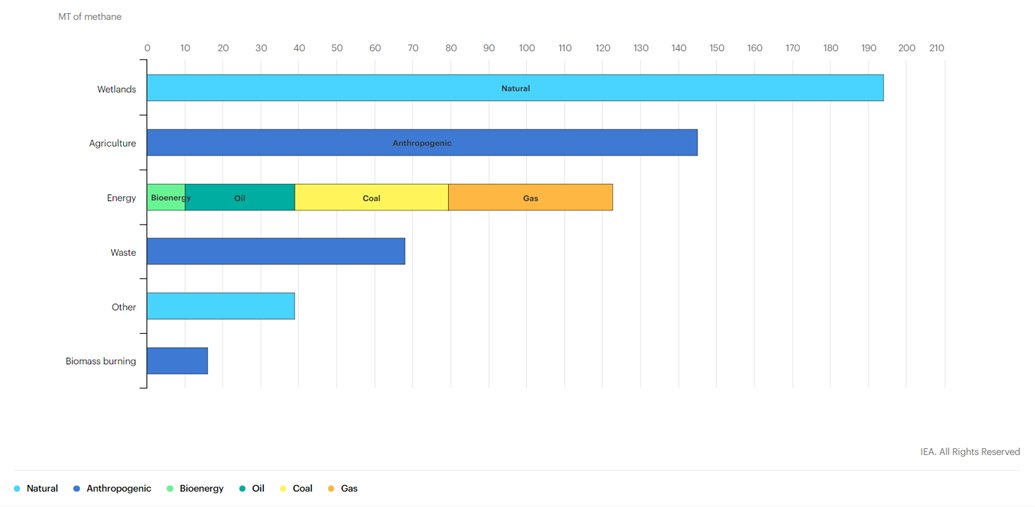
\includegraphics{fig/Methane_by_Source.jpeg}

Methane, the largest component of natural gas, is sometimes called a ``short-lived climate pollutant'' because it remains in the atmosphere for far less time than carbon dioxide, which can remain in the atmosphere for hundreds of years. But methane is also a climate ``super-pollutant,'' 86 times more potent than carbon dioxide at warming the atmosphere over a 20-year period.

Sources of methane include wetlands, rice paddies, livestock, biomass burning, organic waste decomposition and fossil fuel drilling and transport.

\emph{James Hansen}

The methane (CH4) growth rate{[}3{]} is shocking.
A CH4 increase causes tropospheric ozone (O3) and stratospheric water vapor (H2O)
to also increase.
Including these indirect effects, the climate forcing by observed CH4 growth
is half as large as the climate forcing by CO2.

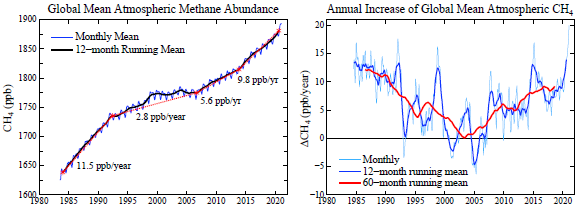
\includegraphics{fig/CH4_Annual_Increase.png}

After CH4 nearly stabilized early this century, growth has returned and recently accelerated to its highest rate in the period of accurate global data, with increased growth at least in part as a result of ``fracking'' for gas and reliance on gas as the complement to intermittent renewable energies.

\href{https://mailchi.mp/caa/the-world-has-cooled-off-whats-the-significance}{James Hansen 13 May 2021}

\hypertarget{global-methane-assessment}{%
\subsubsection{Global Methane Assessment}\label{global-methane-assessment}}

The Global Methane Assessment shows that human-caused methane emissions can be reduced by up to 45 per cent this decade. Such reductions would avoid nearly 0.3°C of global warming by 2045 and would be consistent with keeping the Paris Climate Agreement's goal to limit global temperature rise to 1.5 degrees Celsius (1.5˚C) within reach.

The assessment, for the first time, integrates the climate and air pollution costs and benefits from methane mitigation. Because methane is a key ingredient in the formation of ground-level ozone (smog), a powerful climate forcer and dangerous air pollutant, a 45 per cent reduction would prevent 260 000 premature deaths, 775 000 asthma-related hospital visits, 73 billion hours of lost labour from extreme heat, and 25 million tonnes of crop losses annually.

\href{https://www.ccacoalition.org/en/resources/global-methane-assessment-full-report}{Global Methane Assessment Report}

\href{https://www.inkl.com/news/a-sweeping-u-n-report-says-methane-is-far-worse-for-the-climate-human-health-than-previously-thought}{Inkl: Methane Far Worse}

\hypertarget{cut-methane-now}{%
\subsubsection{Cut Methane Now}\label{cut-methane-now}}

Methane is the biggest and really the only lever we have to slow
temperature rise during the next two decades.

Methane's potency and short atmospheric life make it a key greenhouse gas for policy makers to focus on as a way to combat global warming in the near term because the impact of those cuts will be felt almost immediately.

``If we cut methane emissions substantially during the 2020s, the abundance or concentration in the atmosphere will also drop rapidly during the 2020s,'' said Drew Shindell, an earth science professor at Duke University. ``If we cut CO2 emissions, it takes a long time for actual concentrations to drop, and then longer for the climate to adjust.''

\href{https://insideclimatenews.org/news/20042021/methane-biden-climate-summit/}{Inside}

\hypertarget{spotting-methane-from-space}{%
\subsubsection{Spotting Methane from Space}\label{spotting-methane-from-space}}

Methane is a key driver of climate change, with 80 times the global warming impact of carbon dioxide over a 20-year period. But methane only lingers in the atmosphere for about nine years, compared to a century for CO2.

That means reducing methane emissions from oil and gas wells and pipelines, livestock operations, landfills and other sources around the world will have an outsize impact on reducing global warming.

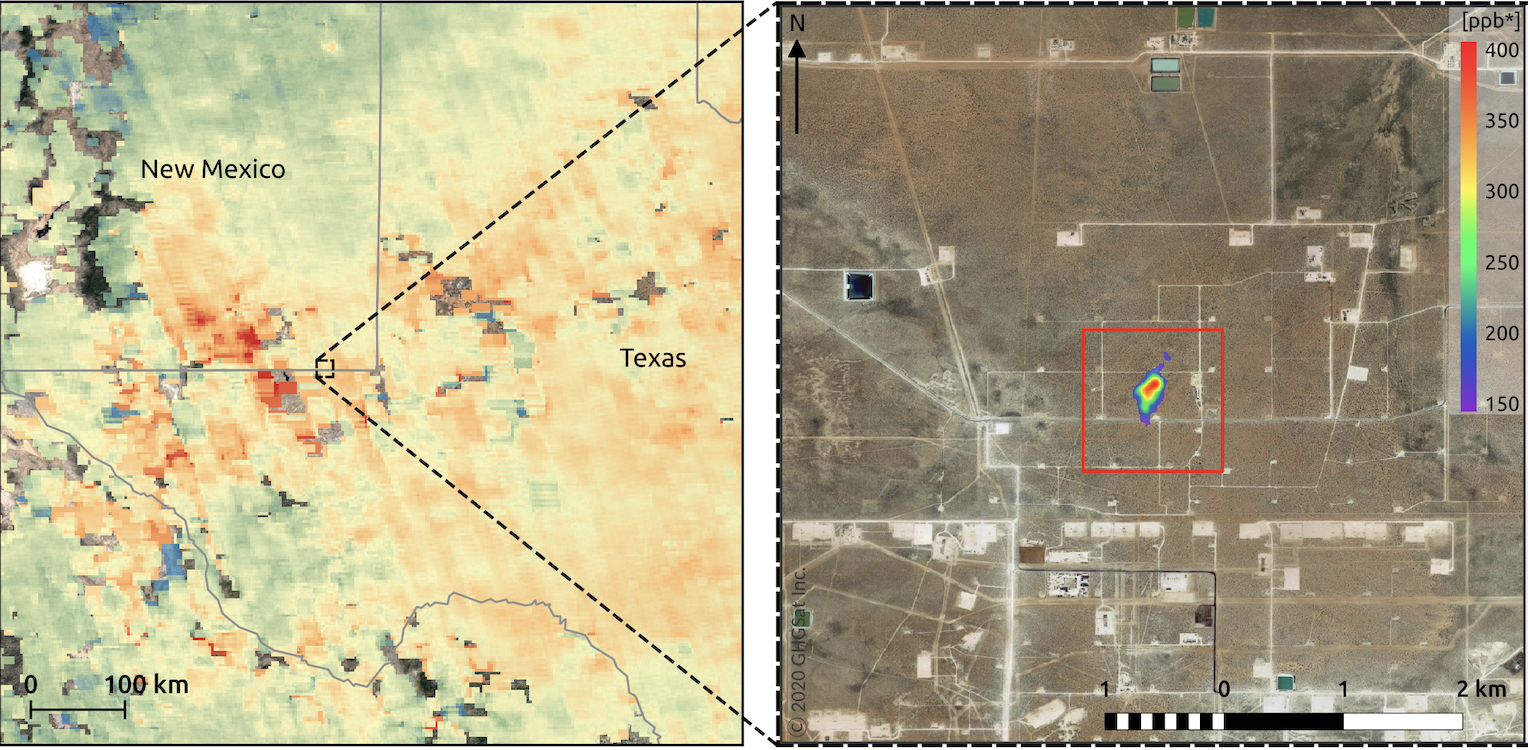
\includegraphics{fig/ESA_Methane_Spotting.png}

Two separate efforts to launch satellites that can scan the globe for methane emissions at a scope and level of detail not possible before, and to share their data with the public.

The first is \href{https://www.methanesat.org/}{MethaneSat}, a subsidiary of the Environmental Defense Fund that is set to launch its satellite in 2022 and start delivering data in 2023. MethaneSat will be able to scan 200-kilometer-wide swaths of the earth with spectrometers that can detect methane at concentrations of 2 to 3 parts per billion, down to resolutions of about 100 meters by 400 meters.
This will be the best performance of any satellite-based methane tracking technology yet launched.

In comparison, the \href{http://www.tropomi.eu/data-products/methane}{Tropomi} sensors on the European Space Agency's Copernicus Sentinel satellite can detect about 11 parts per billion at resolutions of 7 kilometers, and the sensors on satellites operated by Canadian-based company \href{https://www.ghgsat.com/pulse/}{GHGSat} can capture about 55 parts per billion, albeit at much tighter spatial dimensions, down to roughly 25 meters square.

MethaneSat will be able to capture leaks as low as 5 kilograms per hour per square kilometer.

Newly released \href{https://www.edf.org/media/study-cutting-methane-emissions-quickly-could-slow-climate-warming-rate-30}{research} finds that roughly half of global methane emissions can be cut over the next decade at no net cost. Of that low-cost reduction potential, 80 percent could come from the global oil and gas industries.

\href{https://www.canarymedia.com/articles/how-new-satellites-can-drive-action-against-methanes-outsize-impact-on-climate-change/}{CanaryMedia}

\hypertarget{methane-reservoir-laptev-sea}{%
\subsection{Methane Reservoir Laptev Sea}\label{methane-reservoir-laptev-sea}}

Methane bubbles regularly reach the surface of the Laptev Sea in the East Siberian Arctic Ocean (ESAO), each of them a small blow to our efforts to mitigate climate change. The source of the methane used to be a mystery, but a joint Swedish-Russian-U.S. investigation recently discovered that an ancient gas reservoir is responsible for the bubbly leaks.

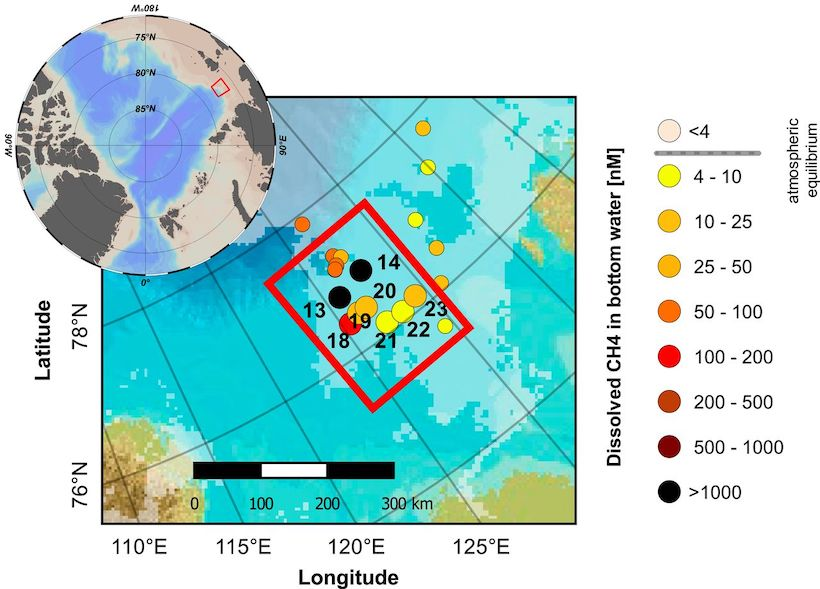
\includegraphics{fig/laptev-sea-methane-map.jpg}

Methane in the Laptev Sea is stored in reservoirs below the sea's submarine permafrost or in the form of methane hydrates---solid ice-like structures that trap the gas inside. It is also produced by microbes in the thawing permafrost itself. Not all of these sources are created equal: Whereas microbial methane is released in a slow, gradual process, disintegrating hydrates and reservoirs can lead to sudden, eruptive releases.

Methane is escaping as the Laptev's submarine permafrost is thawed by the relative warmth of overlying seawater. With an even stronger greenhouse effect than carbon dioxide, methane releases into the atmosphere could substantially amplify global warming.

The source of the methane was an old reservoir, deep below the permafrost.
The big finding was that we really have something that's coming out from a deep pool.
As the permafrost thaws, it opens up new pathways that allow methane to pass through.
There is a risk that this methane release might increase, so it will eventually have a sizable effect on the climate.

It is quite plausible that there are other sources---the thawing permafrost or the hydrates that can be the major source of methane in other parts of this enormous system.

The permafrost is a closed lid over the seafloor that's keeping everything in place. And now we have holes in this lid.

\href{https://eos.org/articles/a-massive-methane-reservoir-is-lurking-beneath-the-sea\#.YJUr2-3rTRI.twitter}{Eos}

\hypertarget{methane-hydrates}{%
\subsection{Methane-Hydrates}\label{methane-hydrates}}

\emph{Ruppel Abstract}

Gas hydrate, a frozen, naturally-occurring, and highly-concentrated form of methane, sequesters significant carbon in the global system and is stable only over a range of low-temperature and moderate-pressure conditions. Gas hydrate is widespread in the sediments of marine continental margins and permafrost areas, locations where ocean and atmospheric warming may perturb the hydrate stability field and lead to release of the sequestered methane into the overlying sediments and soils. Methane and methane-derived carbon that escape from sediments and soils and reach the atmosphere could exacerbate greenhouse warming. The synergy between warming climate and gas hydrate dissociation feeds a popular perception that global warming could drive catastrophic methane releases from the contemporary gas hydrate reservoir. Appropriate evaluation of the two sides of the climate-methane hydrate synergy requires assessing direct and indirect observational data related to gas hydrate dissociation phenomena and numerical models that track the interaction of gas hydrates/methane with the ocean and/or atmosphere. Methane hydrate is likely undergoing dissociation now on global upper continental slopes and on continental shelves that ring the Arctic Ocean. Many factors---the depth of the gas hydrates in sediments, strong sediment and water column sinks, and the inability of bubbles emitted at the seafloor to deliver methane to the sea-air interface in most cases---mitigate the impact of gas hydrate dissociation on atmospheric greenhouse gas concentrations though. There is no conclusive proof that hydrate-derived methane is reaching the atmosphere now, but more observational data and improved numerical models will better characterize the climate-hydrate synergy in the future.

\href{https://agupubs.onlinelibrary.wiley.com/doi/full/10.1002/2016RG000534}{Ruppel (2016) The interaction of climate change and methane hydrates}
\href{pdf/Ruppel_2016_Methane_Hydrates.pdf}{(pdf)}

\hypertarget{methane-emission-rates}{%
\subsection{Methane emission rates}\label{methane-emission-rates}}

\emph{Guardian}

Methane is four times more sensitive to global warming than previously thought, a new study shows. The result helps to explain the rapid growth in methane in recent years and suggests that, if left unchecked, methane related warming will escalate in the decades to come.

The growth of this greenhouse gas -- which over a 20 year timespan is more than 80 times as potent than carbon dioxide -- had been slowing since the turn of the millennium but since 2007 has undergone a rapid rise, with \href{https://gml.noaa.gov/ccgg/trends_ch4/\#:~:text=Global\%20CH4\%20Monthly\%20Means\&text=The\%20Global\%20Monitoring\%20Division\%20of,et\%20al.,\%201994}{measurements from the US National Oceanic and Atmospheric Administration} recording it passing 1,900 parts a billion last year, nearly triple pre-industrial levels.

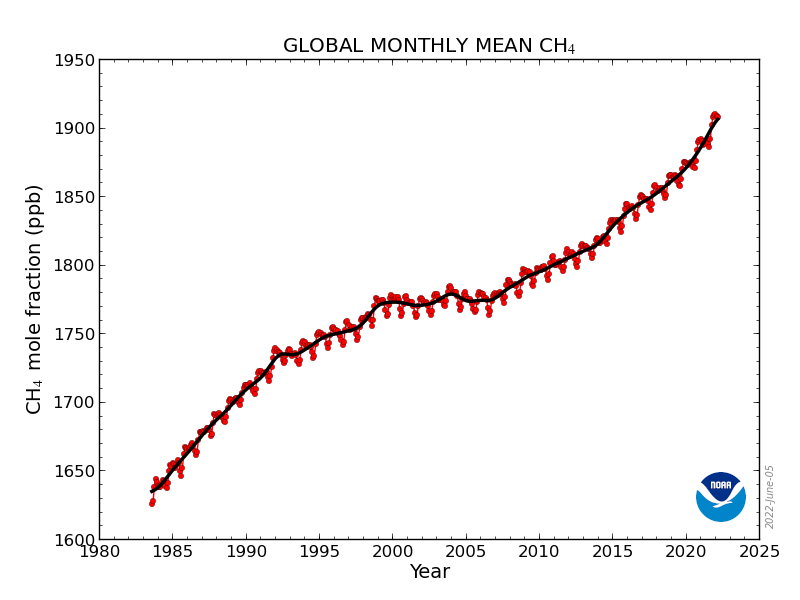
\includegraphics{fig/ch4_trend_all_gl.png}

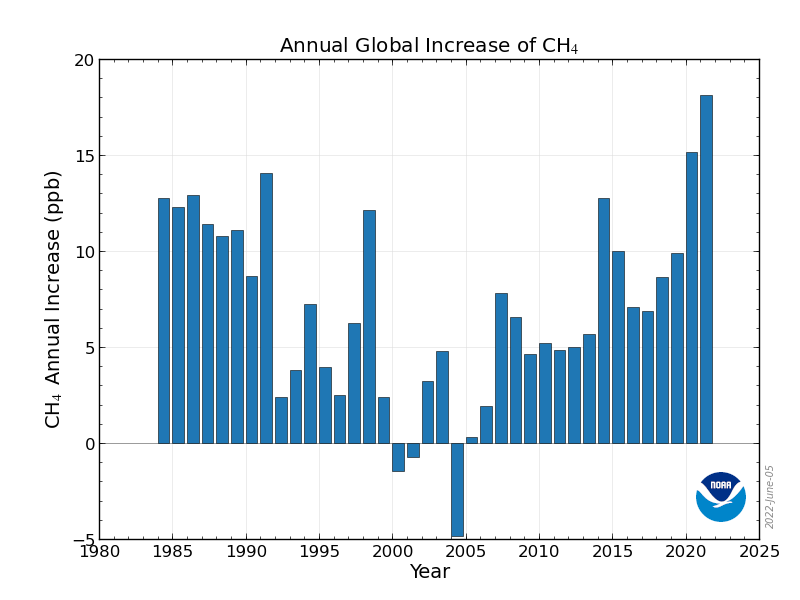
\includegraphics{fig/ch4_gr_gl.png}

About 40\% of methane emissions come from natural sources such as wetlands, while 60\% come from anthropogenic sources such as cattle farming, fossil fuel extraction and landfill sites. Possible explanations for the rise in methane emissions range from expanding exploration of oil and natural gas, rising emissions from agriculture and landfill, and rising natural emissions as tropical wetlands warm and Arctic tundra melts.

But another explanation could be a slowdown of the chemical reaction that removes methane from the atmosphere. The predominant way in which methane is ``mopped up'' is via reaction with hydroxyl radicals (OH) in the atmosphere.

The hydroxyl radical has been termed the `detergent' of the atmosphere because it works to cleanse the atmosphere of harmful trace gases,'' said Redfern. But hydroxyl radicals also react with carbon monoxide, and an increase in wildfires may have pumped more carbon monoxide into the atmosphere and altered the chemical balance. ``On average, a carbon monoxide molecule remains in the atmosphere for about three months before it's attacked by a hydroxyl radical, while methane persists for about a decade. So wildfires have a swift impact on using up the hydroxyl `detergent' and reduce the methane removal.

\href{https://www.theguardian.com/environment/2022/jul/05/global-heating-causes-methane-growth-four-times-faster-than-thought-study}{Guardian (2022) Methane much more sensitive to global heating than previously thought}

\hypertarget{methane-other}{%
\subsection{Methane (other)}\label{methane-other}}

\emph{Guardian}

Another setback has arisen in the attempt to neutralise methane as it escapes from beneath melting Arctic ice. Methane bubble plumes are increasingly being seen in the Arctic, and Wadhams is frustrated that the Intergovernmental Panel on Climate Change (IPCC) has not yet accepted his theory that, as the ice melts, we could face a catastrophic escape of methane that has been stored for 20,000 years. Estimates, he says, range from 50 to 700 gigatonnes, which could ``cause maybe a degree {[}centigrade{]} of warming, more or less instantly'', bringing forward by 15--35 years the average date at which the global mean temperature rise exceeds 2°C above pre-industrial levels.

The best geoengineering prevention for that relies, again, on the ocean. ``If you blow a fine powder, or aerosol, of an iron salt called ferric chloride over the sea surface in the place where methane is bubbling out, it reacts with the methane, producing ferric hydroxide, which dissolves in the water,'' he says.

Frustratingly for the theory's backers, a test voyage this year by the University of Copenhagen found no evidence that it could work efficiently enough to remove the required amounts of the gas.

Guardian{]}(\url{https://www.theguardian.com/environment/2021/jun/23/cloud-spraying-and-hurricane-slaying-could-geoengineering-fix-the-climate-crisis})

\hypertarget{aerosols}{%
\section{Aerosols}\label{aerosols}}

\emph{Hansen}

The global warming acceleration is due to the one huge climate forcing that we have chosen not to measure: the forcing caused by imposed changes of atmospheric aerosols.

It's a shame that we are not measuring the aerosol climate forcing to take advantage of this vast geophysical experiment to improve our understanding. The human-made aerosol forcing is almost as large as the CO2 forcing, but it is of the opposite sign, i.e., aerosols cause cooling.

Aerosols cause cooling by reflecting sunlight to space, thus by itself an increase of aerosols causes a temporary energy imbalance -- more energy going out than coming in. Earth restores energy balance by cooling off, thus reducing heat radiation to space.

The aerosol climate forcing is complex, as the largest part of their effect seems to be via their role as cloud condensation nuclei. Added condensation nuclei tend to make the average cloud particle smaller; that tends to make brighter, longer-lived clouds, but it's a complicated story.

We have so far only felt a fraction of the eventual warming due to the presumed decrease of aerosols of the past several years.

in the absence of adequate aerosol measurements -- let's use Earth's measured energy imbalance to estimate the impact of aerosol reductions on global warming. Earth's energy imbalance is measured to a good accuracy via precise monitoring of the rising global ocean temperature because the ocean is the repository for about 90 percent of the excess energy. Von Schuckmann et al.~(2020){[}4{]} report that the average imbalance over the period 1971-2018 was 0.47 ±0.1 W/m2, but in period 2010-2018 the imbalance was 0.87 ±0.1 W/m2.

Additional information on the energy imbalance is provided by combining the absolute calibration provided by measuring the change in the ocean heat content with the spatial and temporal information provided by satellite-borne radiometers. The CERES (Clouds and the Earth's Radiant Energy System) instruments{[}5{]} measure outgoing radiation -- both reflected sunlight and emitted terrestrial heat radiation. CERES cannot measure the tiny imbalance between the incoming and outgoing fluxes of radiation, but the stability of its sensors is sufficient to infer valuable information about the planet's energy imbalance.

Specifically, the CERES data -- in addition to having temporal variation of Earth's energy imbalance consistent with the ocean data of von Schuckmann et al.~-- show that most of the increased imbalance since 2015 is due to an increase of absorbed solar energy, i.e., a decrease in Earth's reflectivity. That is consistent with the expectation that the largest effect of aerosols on Earth's radiation balance and climate is via their effect on clouds.

We can only infer that Earth's energy imbalance -- which was less than or about half a watt per square meter during 1971-2015 -- has approximately doubled to about 1 W/m2 since 2015. This increased energy imbalance is the cause of global warming acceleration. We should expect the global warming rate for the quarter of a century 2015-2040 to be about double the 0.18°C/decade rate during 1970-2015.

\href{https://mailchi.mp/caa/july-temperature-update-faustian-payment-comes-due?e=96d59a909f}{Hansen (2021) July 2021 temp Update}

\hypertarget{ozone-layer}{%
\section{Ozone Layer}\label{ozone-layer}}

\hypertarget{artic-ozone-hole}{%
\subsection{Artic Ozone Hole}\label{artic-ozone-hole}}

\emph{Berwyn}

The ozone layer, Earth's protection against intense ultraviolet radiation, is at risk, despite the progress made in protecting atmospheric ozone by the 1987 Montreal Protocol.

Warming of the surface of the Arctic is matched by a colder polar vortex high in the atmosphere, which is speeding the breakdown of the Earth's shield against ultraviolet rays.

As greenhouse gases heated the surface of the planet, the researchers said, they have also, during the past 50 years, cooled the upper layers of the atmosphere over the Arctic. In the colder stratosphere, long-lived pollutants like chlorofluorocarbons and halons from refrigerants and industrial solvents break down and release chlorine and bromine, which react with sunlight to destroy ozone.

Concentrations of those pollutants in the atmosphere have decreased by about 10 percent since the ban, allowing the ozone layer above Antarctica to heal over the past 20 years, but progressively colder temperatures in the stratosphere above the Arctic are increasing the destruction of ozone in that region

\href{https://insideclimatenews.org/news/23062021/climate-research-mosaic-arctic-ozone/}{Berwyn (2020) Ozone Alarm in the High North - InsideClimateNews}

\emph{von der Gathen - Abstract}

Chemical loss of Arctic ozone due to anthropogenic halogens is driven by temperature, with more loss occurring during cold winters favourable for formation of polar stratospheric clouds (PSCs). We show that a positive, statistically significant rise in the local maxima of PSC formation potential (PFPLM) for cold winters is apparent in meteorological data collected over the past half century. Output from numerous General Circulation Models (GCMs) also exhibits positive trends in PFPLM over 1950 to 2100, with highest values occurring at end of century, for simulations driven by a large rise in the radiative forcing of climate from greenhouse gases (GHGs). We combine projections of stratospheric halogen loading and humidity with GCM-based forecasts of temperature to suggest that conditions favourable for large, seasonal loss of Arctic column O3 could persist or even worsen until the end of this century, if future abundances of GHGs continue to steeply rise.

\href{https://www.nature.com/articles/s41467-021-24089-6}{von der Gathen (2021) Climate change favours large seasonal loss of Arctic ozone}

\hypertarget{stratosphere-shrinking}{%
\section{Stratosphere shrinking}\label{stratosphere-shrinking}}

The thickness of the atmospheric layer has contracted by 400 metres since the 1980s, the researchers found, and will thin by about another kilometre by 2080 without major cuts in emissions. The changes have the potential to affect satellite operations, the GPS navigation system and radio communications.

The discovery is the latest to show the profound impact of humans on the planet. In April, scientists showed that the climate crisis had shifted the Earth's axis as the massive melting of glaciers redistributes weight around the globe.

The stratosphere extends from about 20km to 60km above the Earth's surface. Below is the troposphere, in which humans live, and here carbon dioxide heats and expands the air. This pushes up the lower boundary of the stratosphere. But, in addition, when CO2 enters the stratosphere it actually cools the air, causing it to contract.

\href{https://www.theguardian.com/environment/2021/may/12/emissions-shrinking-the-stratosphere-scientists-find}{Guardian}

\emph{Pisoft Abstract}

Rising emissions of anthropogenic greenhouse gases (GHG) have led to tropospheric warming and stratospheric cooling over recent decades. As a thermodynamic consequence, the troposphere has expanded and the rise of the tropopause, the boundary between the troposphere and stratosphere, has been suggested as one of the most robust fingerprints of anthropogenic climate change. Conversely, at altitudes above \textasciitilde55 km (in the mesosphere and thermosphere) observational and modeling evidence indicates a downward shift of the height of pressure levels or decreasing density at fixed altitudes. The layer in between, the stratosphere, has not been studied extensively with respect to changes of its global structure. Here we show that this atmospheric layer has contracted substantially over the last decades, and that the main driver for this are increasing concentrations of GHG. Using data from coupled chemistry-climate models we show that this trend will continue and the mean climatological thickness of the stratosphere will decrease by 1.3 km following representative concentration pathway 6.0 by 2080. We also demonstrate that the stratospheric contraction is not only a response to cooling, as changes in both tropopause and stratopause pressure contribute. Moreover, its short emergence time (less than 15 years) makes it a novel and independent indicator of GHG induced climate change.

\href{https://iopscience.iop.org/article/10.1088/1748-9326/abfe2b}{Pisoft}

\hypertarget{n2o}{%
\subsection{N2O}\label{n2o}}

The growth rate of the third strongest greenhouse gas, N2O, does not provide any good news. Its growth rate continues to increase.

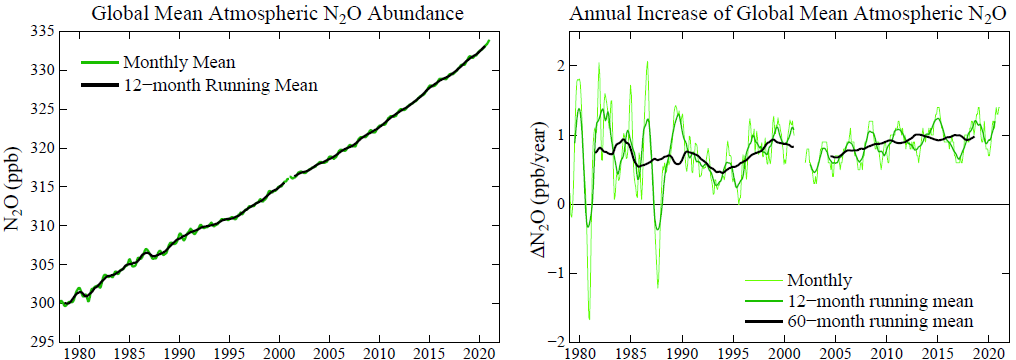
\includegraphics{fig/N2O_Abundance.png}

\href{https://mailchi.mp/caa/the-world-has-cooled-off-whats-the-significance}{James Hansen 13 May 2021}

\hypertarget{contrails}{%
\section{Contrails}\label{contrails}}

\emph{Pearce}

New research shows that condensation trails from aircraft exhaust are playing a significant role in global warming. Experts are concerned that efforts to change aviation engine design to reduce CO2 emissions could actually create more contrails and raise daily temperatures even more.

Like regular cirrus clouds, contrail clouds trap heat radiating from the earth's surface, causing warming in the air below.

Contrails are human-made clouds. They form in air above about 25,000 feet, when that air is moist and colder than -40 degrees Celsius. Like regular clouds, they arise when water vapor, in this case from the engine exhausts, forms into droplets by condensing onto particles in the air, in this case soot from the engines. Within a second, the water droplets freeze to make tiny ice crystals that show up visually as contrails.

If the air is not cool or moist enough, contrails may not form or may disappear quickly. But at other times, they stick around -- either as tight, white lines in the sky, like chalk marks, or gradually spreading to create thin layers of ice clouds. They are similar to natural cirrus clouds and are often called contrail cirrus clouds.

Contrail cirrus clouds cover around 0.6 percent of the global skies at any one time --- nine times the amount covered by contrails themselves. In areas with high amounts of air traffic, they can merge to cover as much as 38,000 square miles, roughly the size of Indiana, and last for many hours or even days.

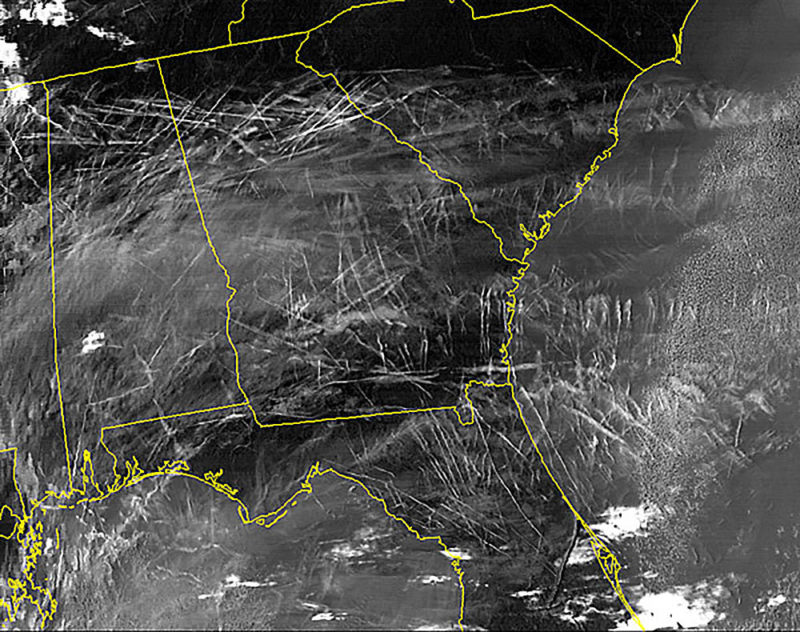
\includegraphics{fig/contrails.jpg}

Like regular cirrus clouds, contrail cirrus clouds have two competing effects on climate. They shade us by reflecting incoming sunlight back into space. But they also trap heat radiating from the earth's surface, so causing warming in the air below.

During the day, cooling compensates part of the warming. But at night, with no sunlight, only the warming effect operates. Red-eye flights are a red light for climate.

The average effect on the earth's radiation balance of contrails and contrail cirrus is 50 milliwatts per square meter of the earth's surface.
The figure is for 2006, the base year for the U.S. Federal Aviation Administration dataset used by the authors. It was double the 24 milliwatts from the CO2 that had accumulated in the atmosphere from a century of aviation (and is a significant part of a total anthropogenic effect at the time of around 1,600 milliwatts).

One is to divert aircraft away from air where contrails are likely to form. This can be done vertically by changing altitude, or horizontally by detouring around the problem air. But aircraft currently fly the shortest routes and at altitudes that minimize fuel burn \ldots controlling contrail formation in this way\ldots{} will almost certainly lead to increases in aircraft CO2 emissions.

A second approach to minimizing contrails is to change fuels --- from kerosene-based fuels to biofuels, hydrogen, liquid natural gas, or even electricity.

Even if fuel changes reduce soot emissions, researchers estimate contrail production will increase by a factor of 2.8 by 2050.

\href{https://e360.yale.edu/features/how-airplane-contrails-are-helping-make-the-planet-warmer}{Pearce (2019) Airplane Contrails make Planet warmer}

\href{https://twitter.com/KenCaldeira/status/1394648353594515460/photo/1}{Kaldeira (twitter thread)}

\hypertarget{clouds}{%
\section{Clouds}\label{clouds}}

\emph{Ceppi Significance}

A key challenge of our time is to accurately estimate future global warming in response to a doubling of atmospheric carbon dioxide---a number known as the climate sensitivity. This number is highly uncertain, mainly because it remains unclear how clouds will change with warming. Such changes in clouds could strongly amplify or dampen global warming, providing a climate feedback. Here, we perform a statistical learning analysis that provides a global observational constraint on the future cloud response. This constraint supports that cloud feedback will amplify global warming, making it very unlikely that climate sensitivity is smaller than 2 °C.

\emph{Ceppi Abstract}

Global warming drives changes in Earth's cloud cover, which, in turn, may amplify or dampen climate change. This ``cloud feedback'' is the single most important cause of uncertainty in Equilibrium Climate Sensitivity (ECS)---the equilibrium global warming following a doubling of atmospheric carbon dioxide. Using data from Earth observations and climate model simulations, we here develop a statistical learning analysis of how clouds respond to changes in the environment. We show that global cloud feedback is dominated by the sensitivity of clouds to surface temperature and tropospheric stability. Considering changes in just these two factors, we are able to constrain global cloud feedback to 0.43 ± 0.35 W⋅m−2⋅K−1 (90\% confidence), implying a robustly amplifying effect of clouds on global warming and only a 0.5\% chance of ECS below 2 K. We thus anticipate that our approach will enable tighter constraints on climate change projections, including its manifold socioeconomic and ecological impacts.

\href{https://www.pnas.org/content/118/30/e2026290118}{Ceppi (2021) Observational evidence that cloud feedback amplifies global warming}

\hypertarget{attributing-emissions}{%
\section{Attributing Emissions}\label{attributing-emissions}}

\hypertarget{norways-responsibility}{%
\subsection{Norway's Responsibility}\label{norways-responsibility}}

\begin{verbatim}
In real life responsibility is more than what is legally binding
\end{verbatim}

The emissions of CO2 that occur within Norway's territory are dwarfed by the emissions that result from combustion of all the oil and gas Norway produces. Because these fossil fuels are exported before being combusted, the emissions are allocated to the accounts of other countries. If Norway had generated electricity from the gas and then exported the electricity, for example, then emissions from that electricity generation would be allocated to Norway's accounts. There is therefore an element of artificiality associated with this allocation. It takes two to tango.

Norway's territorial emissions of CO2 were about 42 Mt in 2019, and over 1971--2019 totalled about 1.9 Gt. In comparison, emissions from Norwegian oil and gas since 1971 have been about 16 Gt. A similar amount (\textasciitilde15 Gt) will be emitted if all remaining Norwegian oil and gas resources are extracted from the continental shelf.

In 2019, emissions from Norwegian oil and gas amounted to 84 tonnes of CO2 for every person in Norway.

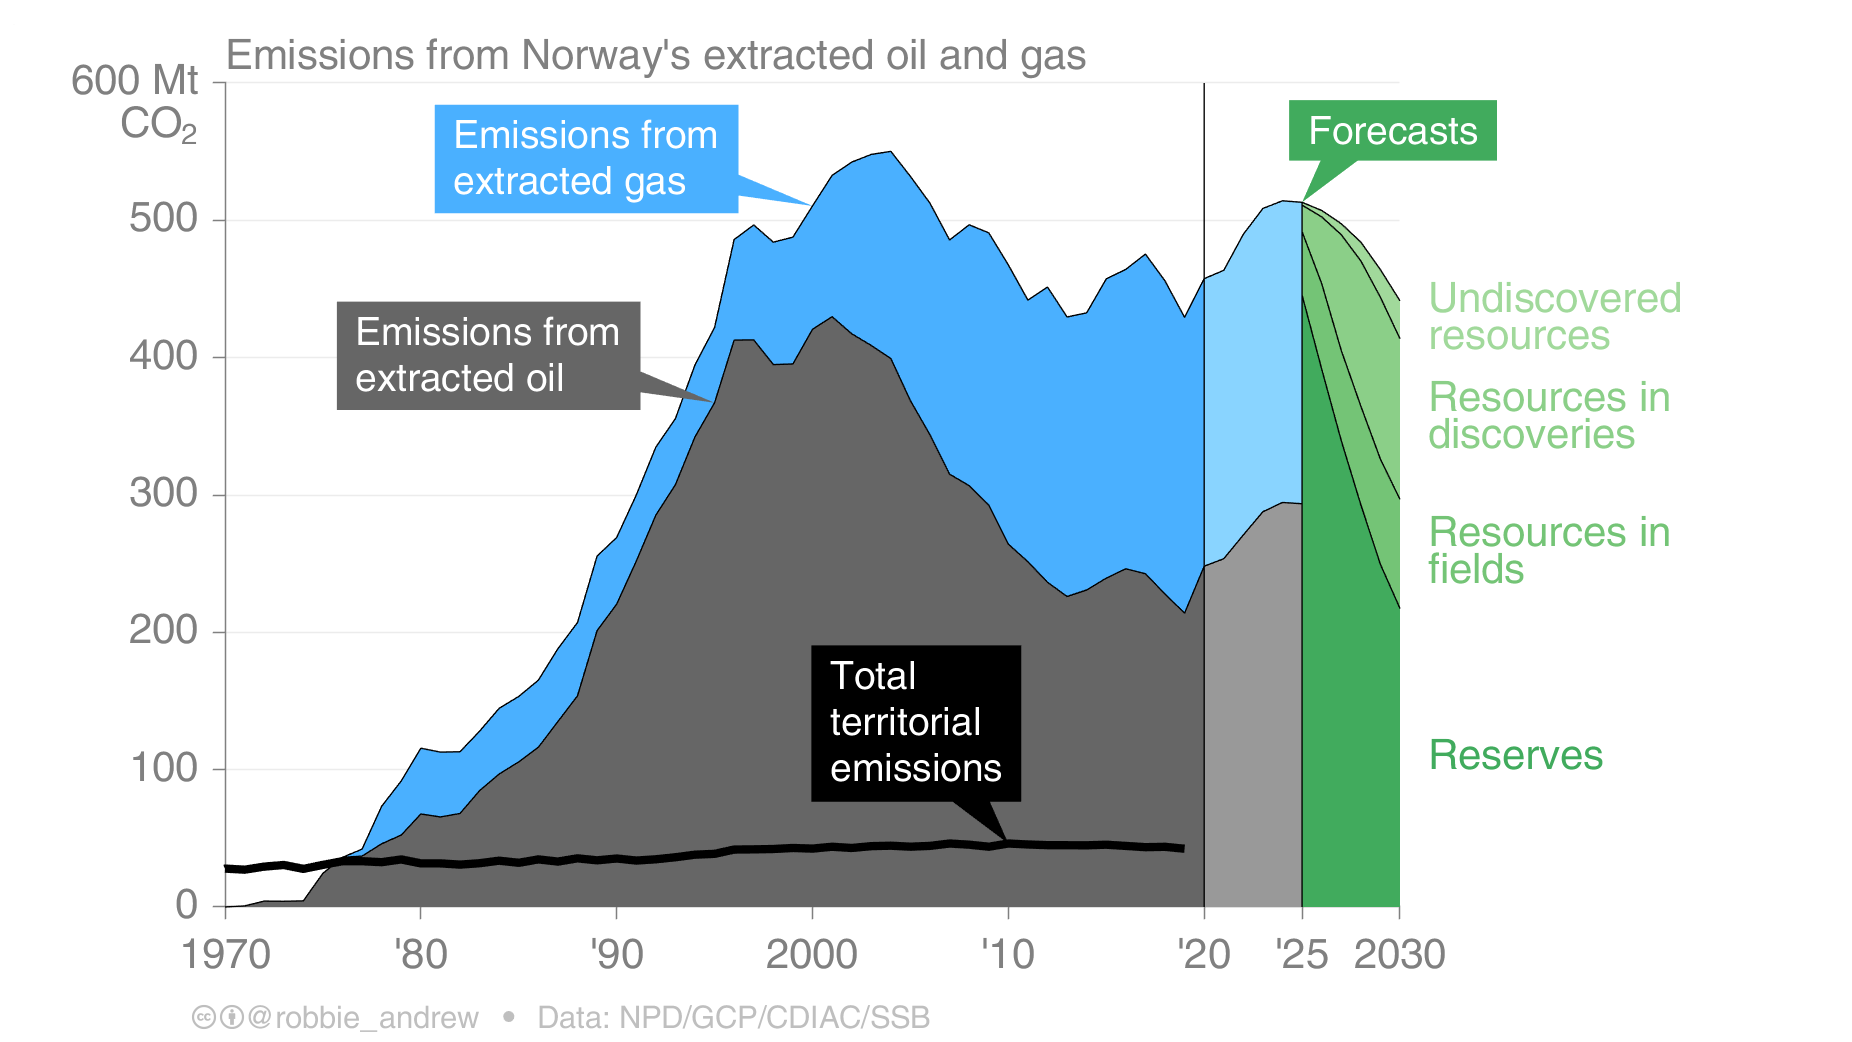
\includegraphics{fig/Emissions_extracted_Oil_Gas_Norway.png}

\href{https://folk.universitetetioslo.no/roberan/t/export_emissions.shtml}{Norways Export Emissions (Robbie Andrew)}

In Norwegian politics, there's been a very successful attempt to separate the discussion of oil policy from the discussion of climate policy. The two were never really tightly linked {[}in the country{]} until roughly the last decade, and this division has become increasingly difficult to maintain.

Norwegian politicians also haven't been alone in creating the conditions that made this division possible. They've been helped immensely by the international climate regime.

From the very beginning of international climate policy, there was this agreement that countries had to account for the emissions that they create when they burn fossil fuels. All the responsibility was placed on the demand side, not the supply side, which was very convenient for Norway.

Europe is the primary market for Norway's oil and gas. But determining the climate effects of Norwegian production is not straightforward. One study has estimated a clear climate benefit from reducing oil output, but the market is complex and the result really depends on your assumptions about how other actors will behave and how the market will evolve over time.

The big irony here is that Norway is a fairly large fossil-fuel producer, but we use relatively few fossil fuels directly in our energy use. Nearly all of our electricity has for a long time come from hydropower. In most years, we even export quite a lot of renewable electricity to our neighbors.
The only place where fossil fuels are used to directly produce energy is to run the platforms offshore. They use gas to run the turbines to get the energy needed for oil and gas production.

The government's new climate plan, which was unveiled just a few days ago, does include a number of new and more aggressive measures to reduce Norway's domestic emissions. The proposal to increase the already quite high CO2 tax on offshore emissions came as something of a surprise, and it is likely to pass even if it is currently being challenged by the industry.

However, it is important to keep in mind that this proposal only targets the production-related emissions of Norwegian oil, not the level of oil that is being extracted and exported. As such, it is in line with the historical separation between climate and oil policymaking, which tends to focus only on emissions happening within Norway and exclude any concern for the climate impact of exported oil and gas.

The Norwegian paradox has worked out fairly well up until the last few years because there has been little focus on the production of fossil fuels, and because Norway is small enough to avoid the scrutiny that some larger nations face. But this is quickly changing, both in the domestic and international political discussion.

There is now a lot more focus on the supply side of fossil fuels than 10 years ago, with several countries like Denmark announcing an end to drilling and new research showing a mismatch between planned fossil-fuel production and ideas such as a ``non-proliferation treaty'' for fossil fuels being floated. The treaty would bring the world together in agreeing to end the use of fossil fuels much like the UN came together to curb the spread of nuclear weapons.

This will make it increasingly hard for Norway to hold on to a leadership claim as long as oil production keeps being expanded into new areas.

\href{https://www.vox.com/22227063/norway-oil-gas-climate-change}{Norways Climate - Petroleum Dilemma (Bard Lahn)}

\hypertarget{global-north-vs-south-responsibility}{%
\subsection{Global North vs South Responsibility}\label{global-north-vs-south-responsibility}}

The global North is responsible for 92\% of total excess carbon dioxide emissions.
Climate breakdown is colonial in character and ultimately requires an anti-colonial struggle in response. (Jason Hickel)

\begin{figure}
\centering
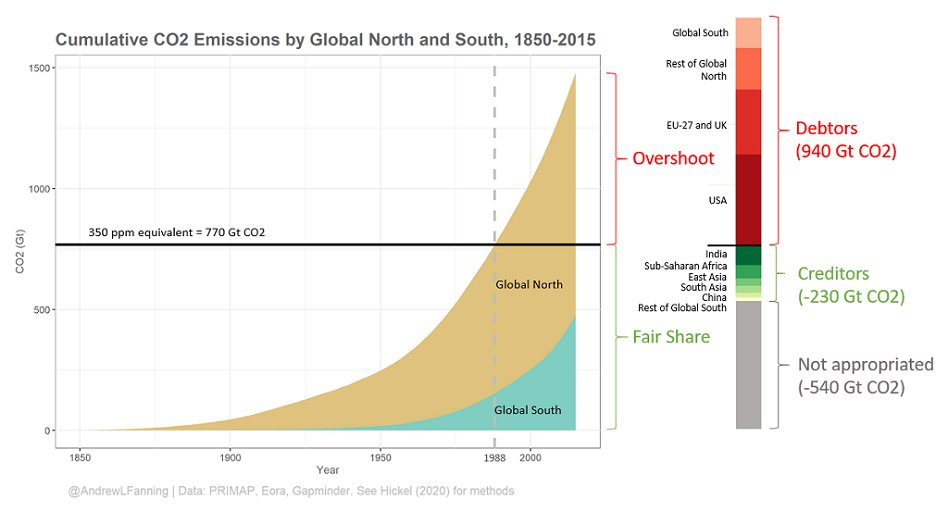
\includegraphics{fig/CO2_Emissions_Global_North_South.jpeg}
\caption{Fig. by \citet{AndrewFanning}}
\end{figure}

\hypertarget{concrete-cement}{%
\subsection{Concrete / Cement}\label{concrete-cement}}

\emph{CanaryMedia}

Concrete is everywhere, and it accounts for 7 to 8 percent of global carbon emissions.

Quick facts about clean concrete for people who don't work with concrete

\begin{itemize}
\tightlist
\item
  Cement is the most carbon-intensive component in concrete. One easy way to lower carbon impact is to stop the common industrial practice of chucking extra cement in the mix. Apparently, this is widespread and results in more cement in the finished product than what the engineers actually asked for.
\item
  Governments are the biggest purchasers of concrete (think highways, roads, bridges). If they start demanding carbon accounting or giving preference to lower-carbon concrete suppliers, it would have an outsize influence on the industry. A bill now up before California's legislature would do just that.
\item
  Another bill in California would cut carbon from concrete by 40 percent by the end of 2035. This one has support from Democrats, Republicans, industry and environmental groups. Crucially, it includes a ``border adjustment mechanism,'' which means the carbon limits apply to imported concrete. That ensures a level playing field for concrete suppliers if the law goes into effect.
\end{itemize}

(Canary Media Newsletter by Julian Spector
1 July 2021 (No Link))

\href{https://www.canarymedia.com/articles/california-considers-ambitious-bills-to-rein-in-carbon-emissions-from-concrete/}{CanryMedia}

\hypertarget{forests}{%
\chapter{Forests}\label{forests}}

\hypertarget{forests-tipping-go-from-sink-to-source-of-co2-due-to-temperature-increase.}{%
\section{Forests tipping: go from sink to source of CO2 due to temperature increase.}\label{forests-tipping-go-from-sink-to-source-of-co2-due-to-temperature-increase.}}

New research shows that Earth's overheated climate will
alter forests at a global scale even more fundamentally,
by flipping a critical greenhouse gas switch in the next few decades.
The study suggests that, by 2040, forests will take up only
half as much carbon dioxide from the atmosphere as they do now,
if global temperatures keep rising at the present pace.

Global warming has contributed to thinning canopies in European forests
and to sudden die-offs of aspen trees in Colorado,
as well as insect outbreaks that are killing trees around the world.
In many places, forests are not growing back.

The data show a clear temperature limit,
above which trees start to exhale more CO2 than they can take in through photosynthesis.
The findings mark a tipping point, of sorts, at which ``the land system will act to accelerate climate change rather than slow it down,''

\href{https://insideclimatenews.org/news/13012021/forests-heat-climate-change/}{Trees From Sink to Source (InsideClimateNews)}

At present, the land provides a ``climate service'' by absorbing
around 30 per cent of the emissions caused by humans each year.

Unlike other tipping elements in the Earth system, the climate tipping point
for the terrestrial biosphere could be exceptionally close --
20-30 years away -- without action.

Plant respiration, the process by which plants produce energy for growth,
causes CO2 to be released into the atmosphere.

The `buffer' or `discount' against carbon emissions that we currently receive from the biosphere is more fragile than we previously realised.

Climate models are tools used by scientists to simulate how the world is likely to respond to greenhouse gas emissions.

However, it is worth noting that the global dataset used in the study
uses ``very few samples from tropical regions''.
This means that it is still not fully understood how tropical forests
are responding to rising temperatures.

\href{https://www.independent.co.uk/environment/climate-change/land-ecosystems-tipping-point-temperature-b1786822.html}{Independent}

\emph{Memo Duffy}

The temperature dependence of global photosynthesis and respiration
determine land carbon sink strength.
While the land sink currently mitigates \textasciitilde30\% of anthropogenic carbon emissions,
it is unclear whether this ecosystem service will persist and
what hard temperature limits, if any, regulate carbon uptake.

The mean temperature of the warmest quarter (3-month period)
passed the thermal maximum for photosynthesis during the past decade.
At higher temperatures, respiration rates continue to rise
in contrast to sharply declining rates of photosynthesis.

Under business-as-usual emissions, this divergence elicits a
near halving of the land sink strength by as early as 2040.

The difference between gross primary productivity
and total ecosystem respiration
(carbon uptake by vegetation minus carbon loss to the atmosphere)
comprises the metabolic component of the land carbon
sink {[}net ecosystem productivity (NEP){]}.

To date, land ecosystems provide a climate regulation service
by absorbing \textasciitilde30\% of anthropogenic emissions annually.
While temperature functions as a key driver
of year-to-year changes in the land carbon sink,
its temperature response is still poorly constrained at biome to global scales,
making the carbon consequences of anticipated warming uncertain.

Like all biological processes, metabolic rates for photosynthesis
and respiration are temperature dependent; they accelerate with in-
creasing temperature, reach a maximum rate, and decline thereafter.

Highly divergent land carbon sink trajectories from Earth system models.

Continued future increases in sink strength due to the CO2 fertilization.

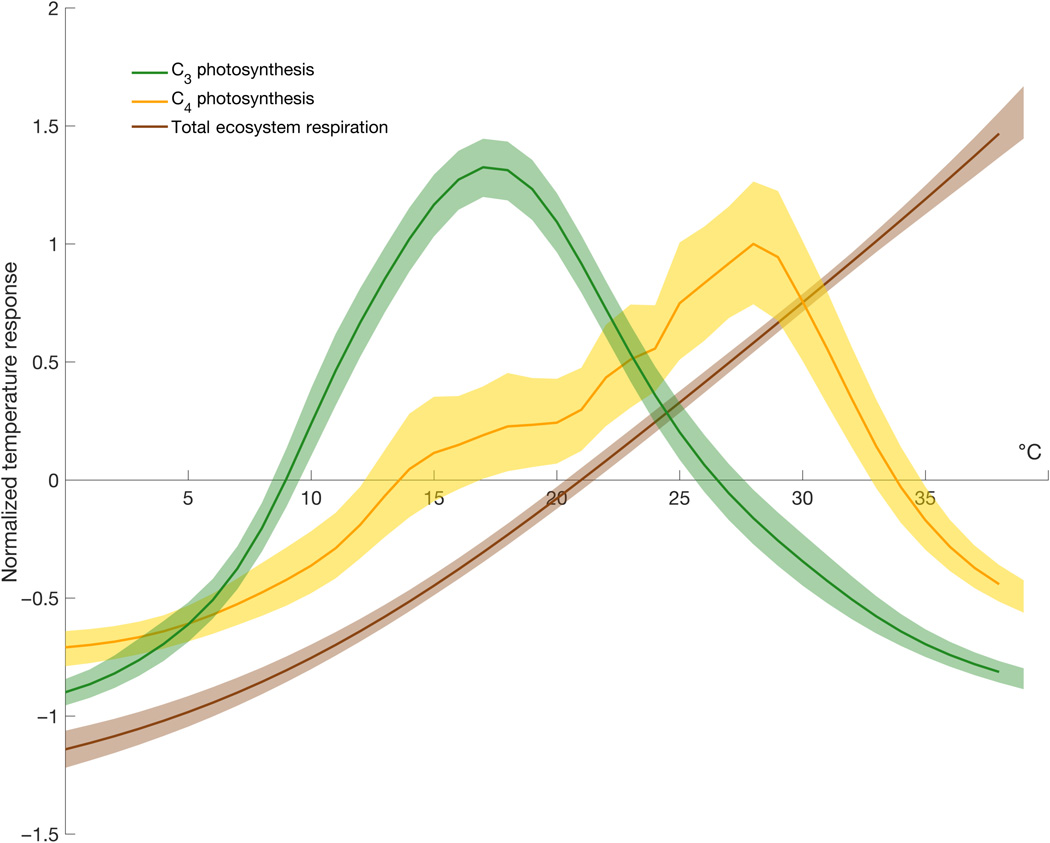
\includegraphics{fig/Photosythesis_Temp_Response.jpg}

The temperature response of global photosynthesis
shows distinct maxima at 18°C for C3 and 28°C for C4 plant systems.
In contrast to photosynthesis, respiration rates increase across
the range of ambient temperatures (up to 38°C),
with no evidence of Tmax or rate decline.
The thermal maxima of leaf and soil respiration reside at \textasciitilde60°-70°C.

Responses diverge at temperatures above Tmax.
The imbalance grows more pronounced as temperature increases.

Current climate mostly lies just below Tmax where slight increases in temperature act as
climate fertilization of land carbon uptake.
Under anticipated warming foreshadowed by historical temperature extremes and coincident
land carbon loss---however, more and more time will be spent above Tmax.
Past this threshold, the land carbon balance will first weaken and
ultimately reverse sign from carbon sink to carbon source.

25°C constitutes a powerful tipping point for the land
sink of carbon and a formidable positive climatic feedback,

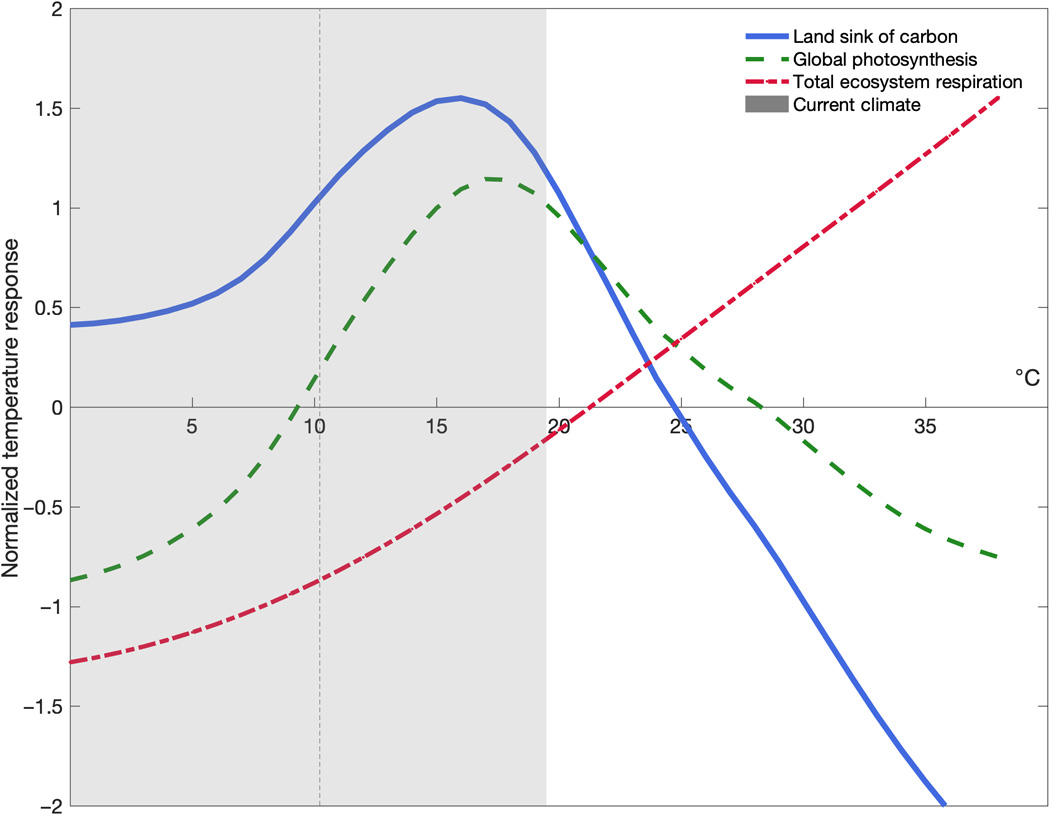
\includegraphics{fig/Land_Sink_of_Carbon.jpg}

Currently, less than 10\% of the terrestrial biosphere experiences
where land carbon uptake is degraded.
For regions that do experience these temperatures,
exposure is limited to 1 to 2 months or
constitutes areas with sparse to no vegetation.

Under business-as-usual emissions, by 2100, up to half
of the terrestrial biosphere could experience temperatures past
the treshold.

The impact of elevated temperatures on the land sink is more than a
function of cumulative area.
Biomes that cycle 40 to 70\% of all terrestrial carbon
including the rainforests of the Amazon and Southeast Asia and
the Taiga forests of Russia and Canada
are some of the first to exceed biome-specific Tmax
for half the year or more.
This reduction in land sink strength is effectively front-loaded
in that a 45\% loss occurs by midcentury,
with only an additional 5\% loss by the end of the century.
These estimates are conservative as they assume
full recovery of vegetation after temperature stress and
ignore patterns and lags in recovery.

In contrast to any CO2 fertilization effect,
anticipated higher temperatures associated with
elevated CO2 could degrade land carbon uptake.
Failure to account for this results in
a gross overestimation of climate change mitigation provided by terrestrial vegetation.

We are rapidly entering temperature regimes where biosphere productivity
will precipitously decline and
calls into question the future viability of the land sink.

\href{https://advances.sciencemag.org/content/7/3/eaay1052}{Duffy(2021) Temperature tipping point of the terrestrial biosphere}
\href{pdf/Duffy_2020_Temperature_Tipping_Point.pdf}{(pdf)}

\hypertarget{plant-and-cut---forest-ccs}{%
\section{Plant and Cut - Forest CCS}\label{plant-and-cut---forest-ccs}}

Wood can also serve purely as a long-term carbon storage device. The key to locking away the carbon is to cut off the oxygen supply to microbes, thereby preventing decomposition.

Natural experiments show how this can be done. 19th-century lumberjacks in the US and Canada frequently stored logs on the surfaces of the Great Lakes or floated them down rivers, some of which ended up sinking along the way. These have remained in such good condition that a modern-day cottage industry has arisen to recover the logs and turn them into everything from hardwood floors to violins. New Zealand has a similar industry with logs that were fortuitously buried in swamps as long as 60,000 years ago.

Based on such examples, scholars have proposed chopping down trees or collecting fallen logs and intentionally stowing them away. That could mean sinking them to the bottom of lakes, interring them in abandoned mines or burying them in specially dug trenches.
The idea hasn't gotten much traction yet, but in 2013, the Quebec Ministry of Agriculture, Fisheries and Food funded a pilot project to dig a trench and bury 35 metric tons of wood. The project came to about \$29 per metric ton of CO2 sequestered, according to government scientist Ghislain Poisson, in line with a theoretical estimate of \$10-\$50.

That is cheaper than most high-tech forms of carbon capture and storage, which usually involve machines that filter carbon out of the air and pump it underground. Sequestering carbon at the typical power plant, where emissions are highly concentrated, runs to \$30-\$91 per metric ton of CO2, but in open air, which is the holy grail, costs theoretically range from \$94-\$232. To help this promising new technology get off the ground (or rather, into the ground), the federal government offers a tax credit of about \$35 for every metric ton of CO2 removed in industrial carbon capture and storage. It's a policy that has enjoyed strong bipartisan support for over a decade.

\href{https://edition.cnn.com/2021/02/10/opinions/climate-plant-and-cut-trees-down-bader/index.html}{Plant and Cut (CNN)}

\hypertarget{deforestation-footprint}{%
\section{Deforestation Footprint}\label{deforestation-footprint}}

(see: env)

\href{Nature,\%20paywall}{Hoang: Mapping Deforestation Footprint}{]}(\url{https://www.nature.com/articles/s41559-021-01417-z})

\hypertarget{groundwater}{%
\chapter{Groundwater}\label{groundwater}}

\hypertarget{groundwater-rise}{%
\section{Groundwater rise}\label{groundwater-rise}}

\emph{Pierre-Louise}

Unlike rising seas, where the dangers are obvious, groundwater rise has remained under the radar. Hydrologists are aware of the problem and it's all over the scholarly research, but it has yet to surface in a significant way outside of those bubbles. Groundwater rise is only briefly mentioned in the most recent edition of the National Climate Assessment, released in 2018; it's absent from many state and regional climate adaptation plans, and even from flood maps.

Any coastal area where ``the land is really flat, and the geology is {[}the kind of{]} loose material that water moves through really easily,'' says Hill, is ``where this is really going to be a problem.'' This includes places like Miami, but also Oakland, California, and Brooklyn, New York. Silicon Valley communities like Mountain View are susceptible to groundwater rise, as is Washington, DC. Worldwide, the area at risk includes portions of northwestern Europe and coastal areas of the United Kingdom, Africa, South America, and Southeast Asia.

And because of how groundwater moves, people who are at risk may not know it until it's too late. ``One of the most important things about the groundwater is that the rising groundwater level precedes any inundation of the surface,'' says Rozell. Put another way, we will experience groundwater flooding long before the ocean comes lapping at our front door.

It might seem puzzling that rising seas could cause groundwater to rise. At first blush the two seem unrelated, but the connection is actually simple. That it has long been ignored reflects our bias toward addressing problems we can easily see.

To understand the link, it first helps to understand a bit about groundwater. The water nestled in sediments underground started as surface water, like rain or snow, and eventually seeped down. A layer of saturated soil rests below a layer of unsaturated soil; the boundary between the two is what's known as the water table. And in many coastal areas this layer of saturated soil, which can be meters thick, rests atop salt water from the ocean. As sea levels rise, the groundwater gets pushed up because salt water is denser than fresh water.

\href{https://www.technologyreview.com/2021/12/13/1041309/climate-change-rising-groundwater-flooding/}{Pierre-Louise (2021) How rising groundwater caused by climate change could devastate coastal communities}

\hypertarget{ice-sheet}{%
\chapter{Ice Sheet}\label{ice-sheet}}

\hypertarget{greenland}{%
\section{Greenland}\label{greenland}}

\emph{Abstract Noel}

Under anticipated future warming, the Greenland ice sheet (GrIS) will
pass a threshold when meltwater runoff exceeds the accumulation of snow,
resulting in a negative surface mass balance (SMB \textless{} 0) and sustained mass loss.

Here we dynamically and statistically downscale the outputs of an
Earth system model to 1 km resolution to infer that a Greenland near‐surface
atmospheric warming of 4.5 ± 0.3 °C---relative to pre‐industrial---is required
for GrIS SMB to become persistently negative.

Climate models from CMIP5 and CMIP6 translate this regional temperature change
to a global warming threshold of 2.7 ± 0.2 °C.
Under a high‐end warming scenario, this threshold may be reached around 2055,
while for a strong mitigation scenario it will likely not be passed.
Depending on the emissions scenario taken, our method estimates a 6‐13 cm sea level rise
from GrIS SMB in the year 2100.

\href{https://agupubs.onlinelibrary.wiley.com/doi/10.1029/2020GL090471}{Noel (2021) Greenland Ice Sheet Loss}
\href{pdf/Noel_2021_Greenland_Ice_Sheet_Loss.pdf}{(pdf)}

\emph{Boers Significance}

It has been suggested that, in response to anthropogenic global warming, the Greenland Ice Sheet may reach a tipping point beyond which its current configuration would become unstable. A crucial nonlinear mechanism for the existence of this tipping point is the positive melt-elevation feedback: Melting reduces ice sheet height, exposing the ice sheet surface to warmer temperatures, which further accelerates melting. We reveal early-warning signals for a forthcoming critical transition from ice-core-derived height reconstructions and infer that the western Greenland Ice Sheet has been losing stability in response to rising temperatures. We show that the melt-elevation feedback is likely to be responsible for the observed destabilization. Our results suggest substantially enhanced melting in the near future.

\emph{Boers Abstract}

The Greenland Ice Sheet (GrIS) is a potentially unstable component of the Earth system and may exhibit a critical transition under ongoing global warming. Mass reductions of the GrIS have substantial impacts on global sea level and the speed of the Atlantic Meridional Overturning Circulation, due to the additional freshwater caused by increased meltwater runoff into the northern Atlantic. The stability of the GrIS depends crucially on the positive melt-elevation feedback (MEF), by which melt rates increase as the overall ice sheet height decreases under rising temperatures. Melting rates across Greenland have accelerated nonlinearly in recent decades, and models predict a critical temperature threshold beyond which the current ice sheet state is not maintainable. Here, we investigate long-term melt rate and ice sheet height reconstructions from the central-western GrIS in combination with model simulations to quantify the stability of this part of the GrIS. We reveal significant early-warning signals (EWS) indicating that the central-western GrIS is close to a critical transition. By relating the statistical EWS to underlying physical processes, our results suggest that the MEF plays a dominant role in the observed, ongoing destabilization of the central-western GrIS. Our results suggest substantial further GrIS mass loss in the near future and call for urgent, observation-constrained stability assessments of other parts of the GrIS.

\href{https://www.pnas.org/content/118/21/e2024192118}{Boers (2021) Western Greenland Ice Sheet is close to a tipping point}

\href{https://www.theguardian.com/environment/2021/may/17/greenland-ice-sheet-on-brink-of-major-tipping-point-says-study}{Guardian}

\hypertarget{antarctica}{%
\section{Antarctica}\label{antarctica}}

\begin{quote}
Antarctica is larger than the US + Mexico and covered by an ice sheet several miles/km thick +80\% of all global fresh water!).
\end{quote}

\includegraphics{fig/Antarctica_Ice_Loss_to_Sea.jpeg}

\hypertarget{sea-level-rise-from-antarctica}{%
\subsection{Sea-level Rise from Antarctica}\label{sea-level-rise-from-antarctica}}

\emph{If it all melted, would raise global sea levels by 57 metres}

\emph{DeConto Abstract}

The Paris Agreement aims to limit global mean warming in the twenty-first century to less than 2 degrees Celsius above preindustrial levels, and to promote further efforts to limit warming to 1.5 degrees Celsius. The amount of greenhouse gas emissions in coming decades will be consequential for global mean sea level (GMSL) on century and longer timescales through a combination of ocean thermal expansion and loss of land ice. The Antarctic Ice Sheet (AIS) is Earth's largest land ice reservoir (equivalent to 57.9 metres of GMSL), and its ice loss is accelerating4. Extensive regions of the AIS are grounded below sea level and susceptible to dynamical instabilities5,6,7,8 that are capable of producing very rapid retreat. Yet the potential for the implementation of the Paris Agreement temperature targets to slow or stop the onset of these instabilities has not been directly tested with physics-based models. Here we use an observationally calibrated ice sheet--shelf model to show that with global warming limited to 2 degrees Celsius or less, Antarctic ice loss will continue at a pace similar to today's throughout the twenty-first century. However, scenarios more consistent with current policies (allowing 3 degrees Celsius of warming) give an abrupt jump in the pace of Antarctic ice loss after around 2060, contributing about 0.5 centimetres GMSL rise per year by 2100---an order of magnitude faster than today. More fossil-fuel-intensive scenarios result in even greater acceleration. Ice-sheet retreat initiated by the thinning and loss of buttressing ice shelves continues for centuries, regardless of bedrock and sea-level feedback mechanisms or geoengineered carbon dioxide reduction. These results demonstrate the possibility that rapid and unstoppable sea-level rise from Antarctica will be triggered if Paris Agreement targets are exceeded.

\href{https://www.nature.com/articles/s41586-021-03427-0}{DeConto (2021) The Paris Climate Agreement and future sea-level rise from Antarctica (Nature Paywall)}

\emph{Abrupt Jump in Ice Loss around 2060}

The world faces a situation where there is an ``abrupt jump'' in the pace of Antarctic ice loss around 2060.

The oceans would have to cool back down before the ice sheet could heal, which would take a very long time. On a societal timescale it would essentially be a permanent change.

This tipping point for Antarctica could be triggered by a global temperature rise of 3C (5.4F) above the preindustrial era feasible by 2100 under governments' current policies.

These ice shelves won't be able to just grow back.

Antarctica is being winnowed away by a warming atmosphere as well as the heating oceans, with warming seawater entering crevasses and gnawing away at ``pinning points'' that hold enormous bodies of ice to submerged bedrock. A rapid acceleration of melting could cause a cascading effect where huge amounts of ice and water flow uninterrupted into the Southern Ocean.
Once in motion, the impacts from such dramatic ice loss would unfurl over centuries.

\href{https://www.theguardian.com/environment/2021/may/05/antarctica-ice-sheet-melting-global-heating-sea-level-rise-study}{Milman (Guardian)}

\hypertarget{thwaites}{%
\subsection{Thwaites}\label{thwaites}}

\emph{Voosen}

An alarming crackup has begun at the foot of Antarctica's vulnerable Thwaites Glacier, whose meltwater is already responsible for about 4\% of global sea level rise. An ice sheet the size of Florida, Thwaites ends its slide into the ocean as a floating ledge of ice 45 kilometers wide. But now, this ice shelf, riven by newly detected fissures on its surface and underside, is likely to break apart in the next 5 years or so, scientists \href{https://agu.confex.com/agu/fm21/meetingapp.cgi/Paper/978762}{reported today at a meeting of the American Geophysical Union}.

\includegraphics{fig/Antarctica_Thwaites.jpeg}

The Thwaites Eastern Ice Shelf (TEIS) buttresses one third of Thwaites Glacier. Removal of TEIS has the potential to increase the contribution of Thwaites Glacier to sea level rise by up to 25\%. Recent research shows that the ice shelf is losing its grip on a submarine shoal that acts as a pinning point and the shear margin that separates TEIS from the Thwaites Glacier Tongue has extended, further weakening the TEIS connection to the pinning point. A sequence of Sentinel-1 radar imagery shows that parallel wing and comb cracks have recently formed rifts at high angles to the main shear margin and are propagating into the central part of the ice shelf at rates as high as 2km per year. We use satellite data, ground-penetrating radar, and GPS measurements to suggest that final collapse of Thwaites Glacier's last remaining ice shelf may be initiated by intersection of rifts with hidden basal crevasse zones within as little as 5 years.

The central part of TEIS has no obvious surface crevasses and smooth surface topography, except for the surface expression of a pronounced basal channel aligned parallel to ice flow. Despite this smooth surface, ground-penetrating radar shows a weak zone of thin ice and complex basal topography, including numerous basal crevasses, that is not in local hydrostatic equilibrium. This local disequilibrium suggests the presence of elevated vertical shear stresses that further weaken this critical part of the ice shelf. GPS stake network observations show no measurable regional strain in the horizontal plane because large-scale flow is being accommodated by the lateral shear margin.

In the near future, the propagating rifts are likely to intersect this weak zone, triggering rifting along the basal crevasses and, subsequently, along the basal channel and a into secondary set of basal crevasses on the eastern side of the basal channel. This ``zigzag'\,' rift sequence would disconnect the main flow from the influence of the pinning point (and compressive arches) and will ultimately lead to a complete disintegration of the ice shelf.

\href{https://www.science.org/content/article/ice-shelf-holding-back-keystone-antarctic-glacier-within-years-failure}{Voosen (2021) Ice shelf holding back keystone Antarctic glacier within years of failure}

\hypertarget{arctic-sea-ice}{%
\section{Arctic Sea Ice}\label{arctic-sea-ice}}

ARCTIC SEA ICE AT RECORD LOW for this time of year. This is an enormous source of amplifying feedback. Losing the remaining Arctic sea ice and its reflection of solar energy back to space would be equivalent to another one trillion tons of CO2.

\includegraphics{fig/Arctic_Sea_Ice_2107715.jpeg}

\href{https://twitter.com/PCarterClimate/status/1416264975522295809/photo/1}{Peter Carter (tweet)}

\hypertarget{ocean}{%
\chapter{Ocean}\label{ocean}}

\emph{IPCC SROCC}

The SROCC is the second special report that the IPCC has published this year and the third of the IPCC's sixth assessment cycle. The \href{https://www.carbonbrief.org/in-depth-qa-the-ipccs-special-report-on-climate-change-and-land}{report on climate change and land} was released in August, while the \href{https://www.carbonbrief.org/in-depth-qa-ipccs-special-report-on-climate-change-at-one-point-five-c}{1.5C report} was published in October 2018. The next special report will be on ``climate change and cities'', which will be published during the seventh assessment cycle of the IPCC -- and so will come after its \href{https://www.ipcc.ch/assessment-report/ar6/}{sixth assessment report (AR6)} in 2021-22.

The special report ``assesses new knowledge'' since the IPCC's fifth assessment report (AR5) -- published in 2013-14 -- and its 1.5C report. It covers ``how the ocean and cryosphere have and are expected to change with ongoing global warming, the risks and opportunities these changes bring to ecosystems and people, and mitigation, adaptation and governance options for reducing future risks''.

The global ocean -- comprising the Arctic, Pacific, Atlantic, Indian, and Southern oceans, as well as their marginal seas -- covers 71\% of the Earth surface, the report notes. It contains ``about 97\% of the Earth's water, supplies 99\% of the Earth's biologically-habitable space, and provides roughly half of the primary production on Earth''.

The cryosphere refers to frozen components of the Earth system that are at or below the land and ocean surface. These include ``snow, glaciers, ice sheets, ice shelves, icebergs, sea ice, lake ice, river ice, permafrost and seasonally frozen ground'', the report notes.

\href{https://www.ipcc.ch/srocc/}{IPCC SROCC (2021)}

\emph{Carbonbrief on SROCC}

``All people on Earth depend directly or indirectly on the ocean and cryosphere,'' the report warns, noting that ``human communities in close connection with coastal environments, small islands, polar areas and high mountains are particularly exposed'' to changes, such as sea level rise and melting glaciers.

It is ``virtually certain'' that the global ocean has warmed unabated since 1970, the report stresses, while ``global warming has led to widespread shrinking of the cryosphere''.

These changes are increasingly pushing adaptation responses ``to their limits'', with the most vulnerable people having ``the lowest capacity'' to respond. Sustainable development and climate change resilience depend ``critically on urgent and ambitious emissions reductions coupled with coordinated sustained and increasingly ambitious adaptation actions''.

In this detailed Q\&A, Carbon Brief unpacks what the report says about how climate change is affecting the Earth's ice and oceans -- and the wider impacts that is having on sea levels, marine life and human society, as well as extreme events and potential ``tipping points''.

\href{https://www.carbonbrief.org/in-depth-qa-the-ipccs-special-report-on-the-ocean-and-cryosphere}{Carbonbrief on SROCC}

\hypertarget{ocean-temperature}{%
\section{Ocean Temperature}\label{ocean-temperature}}

\emph{EPA}

Based on the historical record, increases in sea surface temperature have largely occurred over two key periods: between 1910 and 1940, and from about 1970 to the present. Sea surface temperature appears to have cooled between 1880 and 1910.

Changes in sea surface temperature can alter marine ecosystems in several ways. For example, variations in ocean temperature can affect what species of plants, animals, and microbes are present in a location, alter migration and breeding patterns, threaten sensitive ocean life such as corals, and change the frequency and intensity of harmful algal blooms such as ``red tide.''1 Over the long term, increases in sea surface temperature could also reduce the circulation patterns that bring nutrients from the deep sea to surface waters. Changes in reef habitat and nutrient supply could dramatically alter ocean ecosystems and lead to declines in fish populations, which in turn could affect people who depend on fishing for food or jobs.2,3

Because the oceans continuously interact with the atmosphere, sea surface temperature can also have profound effects on global climate. Increases in sea surface temperature have led to an increase in the amount of atmospheric water vapor over the oceans.4 This water vapor feeds weather systems that produce precipitation, increasing the risk of heavy rain and snow (see the Heavy Precipitation and Tropical Cyclone Activity indicators). Changes in sea surface temperature can shift storm tracks, potentially contributing to droughts in some areas.5 Increases in sea surface temperature are also expected to lengthen the growth season for certain bacteria that can contaminate seafood and cause foodborne illnesses, thereby increasing the risk of health effects.6

\includegraphics{fig/sea_surface_tmp_2.png}

\href{https://www.epa.gov/climate-indicators/climate-change-indicators-sea-surface-temperature}{EPA}

\emph{IUCN}

The ocean absorbs vast quantities of heat as a result of increased concentrations of greenhouse gases in the atmosphere, mainly from fossil fuel consumption. The Fifth Assessment Report published by the Intergovernmental Panel on Climate Change (IPCC) in 2013 revealed that the ocean had absorbed more than 93\% of the excess heat from greenhouse gas emissions since the 1970s. This is causing ocean temperatures to rise.

Data from the US National Oceanic and Atmospheric Administration (NOAA) shows that the average global sea surface temperature -- the temperature of the upper few metres of the ocean -- has increased by approximately 0.13°C per decade over the past 100 years. A 2012 paper published in the journal Geophysical Research Letters revealed that the deep ocean is also affected, with one third of the excess heat absorbed 700 m below the sea surface. Modelling studies published in IPCC's 2013 Report predict that there is likely to be an increase in mean global ocean temperature of 1-4oC by 2100.

The ocean's ability to absorb excess heat has shielded humans from even more rapid changes in climate. Without this oceanic buffer, global temperatures would have risen much more than they have done to date. IPCC's Fourth Assessment Report published in 2007 estimated that the Earth had experienced a warming of 0.55°C since the 1970s. According to an analysis by the Grantham Institute, if the same amount of heat that has gone into the top 2,000 m of the ocean between 1955 and 2010 had gone into the lower 10 km of the atmosphere, the Earth would have seen a warming of 36°C.

Ocean warming leads to deoxygenation -- a reduction in the amount of oxygen dissolved in the ocean -- and sea-level rise -- resulting from the thermal expansion of sea water and continental ice melting. The rising temperatures, coupled with ocean acidification (the decrease in pH of the ocean due to its uptake of CO2), affect marine species and ecosystems and, consequently, the fundamental benefits humans derive from the ocean.

Marine fishes, seabirds and marine mammals all face very high risks from increasing temperatures, including high levels of mortalities, loss of breeding grounds and mass movements as species search for favourable environmental conditions. Coral reefs are also affected by increasing temperatures which cause coral bleaching and increase their risk of mortality.

A 2012 report by the Food and Agriculture Organization of the United Nations estimates that marine and freshwater capture fisheries and aquaculture provide 4.3 billion people with about 15\% of their animal protein. Fisheries and aquaculture are also a source of income for millions of people worldwide. By altering distributions of fish stocks and increasing the vulnerability of fish species to diseases, ocean warming is a serious risk to food security and people's livelihoods globally. Economic losses related to ocean warming are likely to run from tens to hundreds of millions of dollars.

Rising temperatures also affect vegetation and reef-building species such as corals and mangroves, which protect coastlines from erosion and sea-level rise. Rising sea levels and erosion will particularly affect low-lying island countries in the Pacific Ocean, destroying housing and infrastructure and forcing people to relocate.

The rise in sea surface temperatures is causing more severe hurricanes and the intensification of El Niño events bringing droughts and floods. This can have significant socio-economic and health effects in some regions of the world.

Warming ocean temperatures are linked to the increase and spread of diseases in marine species. Humans risk direct transmission of these diseases when consuming marine species, or from infections of wounds exposed in marine environments.

\includegraphics{fig/sea_surface_tmp.png}

\href{https://www.iucn.org/resources/issues-briefs/ocean-warming}{IUCN}

\hypertarget{deep-ocean-heat-content}{%
\subsection{Deep Ocean Heat Content}\label{deep-ocean-heat-content}}

\emph{Bagnell Abstract}

The historical evolution of Earth's energy imbalance can be quantified by changes in the global ocean heat content. However, historical reconstructions of ocean heat content often neglect a large volume of the deep ocean, due to sparse observations of ocean temperatures below 2000 m. Here, we provide a global reconstruction of historical changes in full-depth ocean heat content based on interpolated subsurface temperature data using an autoregressive artificial neural network, providing estimates of total ocean warming for the period 1946-2019. We find that cooling of the deep ocean and a small heat gain in the upper ocean led to no robust trend in global ocean heat content from 1960-1990, implying a roughly balanced Earth energy budget within −0.16 to 0.06 \(Wm^{−2}\) over most of the latter half of the 20th century. However, the past three decades have seen a rapid acceleration in ocean warming, with the entire ocean warming from top to bottom at a rate of 0.63 ± 0.13 \(Wm^{−2}\). These results suggest a delayed onset of a positive Earth energy imbalance relative to previous estimates, although large uncertainties remain.

\emph{Bagnell Memo}

Over the past 15 years, the Argo program5 has deployed thousands of autonomous floats which provide continuous observations of the temperature in the upper half of the ocean, to a depth of 2000 m. This has allowed for a convergence in estimates of OHC over the last fifteen years2,5 and increased confidence in calculations of the ongoing EEI in light of independent confirmation from modern satellite observations2,6,7. However, several challenges exist for reducing uncertainty in estimates of total ocean warming and extending it over longer time periods. First, the deep ocean below 2000 m remains poorly observed, even during the Argo era, which leads to additional uncertainty on current estimates of total warming. While absolute temperature changes in the deep ocean are small8, the large volume of the ocean below 2000 m makes it a potentially meaningful contributor to the global heat inventory. Repeat hydrographic sampling indicates that the deep ocean may be warming significantly in some regions9, particularly the Southern Ocean8, whereas other regions may still be cooling as a response to cold periods in the past millennium10, making it critical to include the heat content of the deep ocean in global estimates of ocean warming. The second issue is that, prior to 2005, data collection was conducted primarily by scientific research vessels and ships of opportunity, leaving areas outside of major trade routes or research transects with few direct observations2,11. This leaves large gaps in the observational record that must be filled in order to estimate OHC.

Several methods have been devised to overcome these gaps in ocean temperature observations and to produce estimates of historical changes in OHC. One common approach applies objective mapping to interpolate the sparse temperature records in space and time. However, while these objective mapping products can reconstruct ocean temperatures back to \textasciitilde1950, they do not extend below 2000 m due to the sparse sampling at these depths. Dynamical data-assimilation models offer an alternative approach to objective mapping and provide full-depth estimates of OHC, but data sparsity means these models are poorly constrained at depth, leading to large cross-model varianc. Another approach based on the passive transport of surface temperature anomalies into the interior ocean can also reconstruct full-depth temperature anomalies and OHC changes, but relies on the potentially incorrect assumption of steady-state circulation16 and is sensitive to the initial condition used in the simulation10,16 and to poorly known surface ocean temperatures dating back several millennia. Finally, statistical methods have been used to detect large-scale trends in the deep ocean temperature from repeat hydrographic sampling, but these have coarse spatial resolution and do not cover the period prior to the mid-1980s. An interpolation product based on in situ temperature data that covers the deep ocean below 2000 m, allowing for a full-depth OHC estimate, remains crucial to reliably estimating historical changes in EEI.

Here, we interpolate historical ocean temperature data using an autoregressive artificial neural network (ARANN) to produce a single consistent estimate of the top-to-bottom OHC change for 1946--2019 using in situ temperature data from the World Ocean Database.
This approach adapts an established machine learning method to perform an iterative autoregression that adjusts spatio-temporal correlation scales over time from the in situ temperature data itself, and effectively propagates information from well-sampled times and regions to more sparsely sampled areas to produce global maps of temperature anomalies at roughly annual resolution.

\includegraphics{fig/deep_ocean_cooling.png}

\emph{Figure: Estimates of ocean heat content (OHC) changes for a the global ocean from the surface to seafloor, b the upper 700 m of the ocean, c the depth range 700--2000 m, and (d) the depth range 2000--5500 m. The mean estimates derived from this study (ARANN, blue) are shown with shading covering two standard deviations from the mean over the 240 ARANN ensemble members. The zero anomaly is defined such that the mean OHC of the ARANN estimate for the period 1946--2019 is zero. Also shown are the mean OHC anomaly from the IAP11 (red), NOAA12 (yellow), and JMA13 (purple) objective mapping products, which cover the 0--2000 m depth interval as shown in (b)--(c). These products have been adjusted to the mean ARANN OHC anomaly for 2005--2019. Shown for a the full ocean depth and d the deep ocean are OHC anomalies from passive ocean heat uptake models using Green's functions (GF)16 (light blue) and an optimized mixing model (OPT-0015)10 (green). The passive ocean heat uptake products are adjusted to the mean ARANN anomaly for 1955--1985. Repeat hydrographic sampling (RHS) gives temperature trends since 1985 in the deep ocean9 (maroon; d). The RHS method gives a linear trend from 1985 to 2000 and from 2000 to 2015, which has been adjusted to the mean ARANN anomaly for 1985--2015.}

\href{https://www.nature.com/articles/s41467-021-24472-3}{Bagnell (2021) 20th century cooling of the deep ocean contributed to delayed acceleration of Earth's energy imbalance}
\href{pdf/Bagnell_2021_Deep_Ocean_Cooling.pdf}{(pdf)}

\href{https://eos.org/articles/deep-ocean-cooling-may-have-offset-global-warming-until-1990}{EOS on Bagnell}

\hypertarget{ocean-acidification}{%
\section{Ocean Acidification}\label{ocean-acidification}}

\emph{Mackie}

Our goal is to provide you with the background to understand the chemical and physical
processes behind ocean acidification. This will allow you to evaluate the commentary on the
web. We were motivated to write the series by the increasing number comments and posts
in the blogosphere based on misconceptions about ocean acidification.
However, despite taking 18 posts and 18,000 words we have only scratched the surface of
the chemistry. This is not surprising as the concepts we have introduced do not stand alone.
Inevitably we have had to leave some things out and simplified others. For each concept we
have explained a dozen more cry out for their 15 minutes. Here is a negligently incomplete
list of a further 18 Quite Important concepts -- each deserving of at least a post -- that we
didn't mention or skipped lightly over. There are hundreds more.

\begin{quote}
δ 13 C, Ψ, Activity coefficients and when and how to use them, Alkalinity: A really useful definition for
alkalinity (i.e.~one that is a measurable quantity), Buffer theory, Burial of CaCO 3 sediments, Carbon vs.
oxygen stoichiometry for combustion of different fossil fuels, Congruent/incongruent dissolution,
Conservative ions and charge balance in seawater, Dissolution of CaCO 3 above the lysocline, DOM,
Fugacity, Inhibition of precipitation, Mass accumulation rate for CaCO 3 sediments, Mixed carbonates
(incorporation of other elements), Net global production of CaCO 3 , different pH scales, Revelle Factor.
\end{quote}

\includegraphics{fig/carbon_reservoirs.png}

\emph{Figure: Carbon reservoirs as preindustrial size (blue circles) and modern size (red circles) with
change since the industrial revolution (black circles). Numbers give size of preindustrial with
amount of change (+ or --) and also express the change as a \%. Size in gigatons of carbon = Gt
C. (1 Gt = 1,000 million tons, i.e.~billion tons).}

\emph{Mackie Memo}

The definition of an acid (in aqueous chemistry) is a substance that
gives (or donates) an \(H^{+}\) (proton) to water to form \$H\_\{3\}O\^{}\{+\} ,
while a base takes (or accepts) the proton.
This means that each acid (or base) reacts with a base (or acid) to produce another
acid-base pair.

Naive application of Le Chatelier's principle is not good enough for complex chemistry.
Le Chatelier's Principle is a way to predict how a see-saw
like equilibrium reaction responds when it is disturbed. It is a useful way to consider simple
reactions. However, Le Chatelier's principle only applies to single-step chemical reactions. It
can't be applied in a simple way to coupled or sequential reactions.

\href{pdf/Mackie_2011_Ocean_Acidification_Intro.pdf}{Mackie (2011) OA not not OK An introduction to the chemistry of Ocean Acidification (pdf)}
\href{https://skepticalscience.com/Mackie_OA_not_OK_post_0.html}{Mackie - Individual Chapters on SkepticalScience}

\hypertarget{outgassing}{%
\subsection{Outgassing}\label{outgassing}}

\emph{Sealevel.info}

Mankind is currently adding about 5 ppmv of CO2 (about 10½ PgC) to the atmosphere each year, but the atmospheric CO2 level is only rising at a rate of about 2.5 ppmv per year. The difference is the rate at which natural negative feedbacks (mainly terrestrial greening and absorption by the oceans) remove CO2 from the air: currently about 2.5 ppmv per year.

However, the solubility of gases like CO2 (or CH4) in water does decrease as the water gets warmer (per the temp­er­a­ture depen­dence of Henry's law), so as the oceans warm they would outgas CO2, if nothing else changed. The capacity of the water to hold dissolved CO2 decreases by about 3\% per 1°C by which the water warms.

\includegraphics{fig/CO2_solubility_in_water.png}

So, when the oceans are absorbing CO2, as is currently the case in most places other than the tropics, if the water warms then the oceans absorb CO2 slightly more slowly.

The effect of temperature change on the solubility of gases in water is surely one of the reasons that atmospheric CO2 levels swing up \& down by about 90 ppmv over glaciation/deglaciation cycles. (There are almost certainly also biological {[}2{]} and/or ice sheet burial mechanisms at work, which increase the magnitude of glacial-interglacial CO2 swings.)

The CO2, in turn, works as a GHG to cause warming. That is a slight positive feedback mechanism.

That positive feedback loop is undoubtedly one of the causes for the apparent hysteresisin the temperature and CO2 records: Over the last million years, the Earth's climate has tended to be either mild, as in our current interglacial (the Holocene), or, more of the time, heavily glaciated and cold, with relatively brief, unstable transitions between.

\href{https://sealevel.info/atmospheric_co2_increase_is_not_from_ocean_outgassing.html}{Sealevel.info}

\hypertarget{ocean-atmosphere-carbon-balance}{%
\section{Ocean-Atmosphere Carbon Balance}\label{ocean-atmosphere-carbon-balance}}

\emph{NASA}

For eons, the world's oceans have been sucking carbon dioxide out of the atmosphere and releasing it again in a steady inhale and exhale. The ocean takes up carbon dioxide through photosynthesis by plant-like organisms (phytoplankton), as well as by simple chemistry: carbon dioxide dissolves in water. It reacts with seawater, creating carbonic acid. Carbonic acid releases hydrogen ions, which combine with carbonate in seawater to form bicarbonate, a form of carbon that doesn't escape the ocean easily.

\includegraphics{fig/ocean_carbon_uptake.jpg}

\emph{Figure: The concentration of carbon dioxide (CO2) in ocean water (y axis) depends on the amount of CO2 in the atmosphere (shaded curves) and the temperature of the water (x axis). This simplified graph shows that as atmospheric CO2 increases from pre-industrial levels (blue) to double (2X) the pre-industrial amounts (light green), the ocean CO2 concentration increases as well. However, as water temperature increases, its ability dissolve CO2 decreases. Global warming is expected to reduce the ocean's ability to absorb CO2, leaving more in the atmosphere\ldots which will lead to even higher temperatures.}

As we burn fossil fuels and atmospheric carbon dioxide levels go up, the ocean absorbs more carbon dioxide to stay in balance. But this absorption has a price: these reactions lower the water's pH, meaning it's more acidic. And the ocean has its limits. As temperatures rise, carbon dioxide leaks out of the ocean like a glass of root beer going flat on a warm day. Carbonate gets used up and has to be re-stocked by upwelling of deeper waters, which are rich in carbonate dissolved from limestone and other rocks.

In the center of the ocean, wind-driven currents bring cool waters and fresh carbonate to the surface. The new water takes up yet more carbon to match the atmosphere, while the old water carries the carbon it has captured into the ocean.

The warmer the surface water becomes, the harder it is for winds to mix the surface layers with the deeper layers. The ocean settles into layers, or stratifies. Without an infusion of fresh carbonate-rich water from below, the surface water saturates with carbon dioxide. The stagnant water also supports fewer phytoplankton, and carbon dioxide uptake from photosynthesis slows. In short, stratification cuts down the amount of carbon the ocean can take up.

The ocean does not take up carbon uniformly. It breathes, inhaling and exhaling carbon dioxide. In addition to the wind-driven currents that gently stir the center of ocean basins (the waters that are most limited by stratification), the ocean's natural, large-scale circulation drags deep water to the surface here and there. Having collected carbon over hundreds of years, this deep upwelling water vents carbon dioxide to the atmosphere like smoke escaping through a chimney. The stronger upwelling brought by the cold phase of the Pacific Decadal Oscillation apparently enhanced the size of the chimney and let more carbon escape to the atmosphere.

\includegraphics{fig/ocean_circulation_carbon_sinks.jpg}

\emph{Figure: The global oceans are connected by deep currents (blue lines) and surface currents (red). Carbon from the atmosphere enters the ocean depths in areas of deep water formation in the North Atlantic and offshore of the Antarctic Peninsula. Where deep currents rise towards the surface, they can release ``fossil'' carbon dioxide stored centuries ago.}

After 30 years of measurements, the ocean carbon community is realizing that tracking human-induced changes in the ocean is not as easy as they thought it would be. It wasn't a mere matter of measuring changes in carbon concentrations in the ocean over time because the natural carbon cycle in the ocean turned out to be a lot more variable than they imagined. ``We discovered that natural processes play such an important role that the signals they generate can be as large as or larger than the anthropogenic signal,'' says Feely. ``Now we are trying to address how these decadal changes affect the uptake of carbon. Once we account for these processes, we can remove them from the data set and calculate the anthropogenic carbon dioxide as the residual.'' But to track the increasingly complicated carbon balance sheet, the ocean community needed models, mathematical simulations of the natural world.

\ldots{}

Stratification might wind up having competing effects on the overall carbon cycle, with saturation slowing carbon dioxide uptake in surface waters, but also suppressing venting.

``The link between the destruction of the ozone layer, the changing wind patterns, and the impact on the carbon cycle is the thing that makes Le Quéré's paper unique,'' says Feely. ``It links back to man-made impacts on the climate.'' The idea that the man-made ozone hole and global warming have changed the Southern Ocean carbon sink is ``disturbing on the one hand, but extremely interesting also,''

Scientists realized that to understand the ocean carbon cycle, they are going to have to look for the human fingerprint in ocean circulation and biology, not just in ocean chemistry.

\href{https://earthobservatory.nasa.gov/features/OceanCarbon}{NASA Earth Observatory}

\emph{Water Encyclopedia}

Of the three places where carbon is stored---atmosphere, oceans, and land biosphere---approximately 93 percent of the CO 2 is found in the oceans. The atmosphere, at about 750 petagrams of carbon (a petagram {[}Pg{]} is 10 15 grams), has the smallest amount of carbon.

Approximately 90 to 100 Pg of carbon moves back and forth between the atmosphere and the oceans, and between the atmosphere and the land biosphere. Although these exchange rates are large relative to the total amount of carbon stored in the atmosphere, the concentration of CO 2 was constant.

All trees, nearly all plants from cold climates, and most agricultural crops respond to increasing atmospheric CO 2 levels by increasing the amount of CO 2 they take up for photosynthesis .

The oceans contain about 50 times more CO 2 than the atmosphere and 19 times more than the land biosphere. CO 2 moves between the atmosphere and the ocean by molecular diffusion when there is a difference between CO 2 gas pressure (pCO 2 ) between the atmosphere and oceans. For example, when the atmospheric pCO 2 is higher than the surface ocean, CO 2 diffuses across the air-sea boundary into the sea water.
The oceans are able to hold much more carbon than the atmosphere because most of the CO 2 that diffuses into the oceans reacts with the water to form carbonic acid and its dissociation products, bicarbonate and carbonate ions . The conversion of CO 2 gas into nongaseous forms such as carbonic acid and bicarbonate and carbonate ions effectively reduces the CO 2 gas pressure in the water, thereby allowing more diffusion from the atmosphere.

The oceans are mixed much more slowly than the atmosphere, so there are large horizontal and vertical changes in CO 2 concentration. In general, tropical waters release CO 2 to the atmosphere, whereas high-latitude oceans take up CO 2 from the atmosphere. CO 2 is also about 10 percent higher in the deep ocean than at the surface. The two basic mechanisms that control the distribution of carbon in the oceans are referred to as the solubility pump and the biological pump.

Solubility Pump.

The solubility pump is driven by two principal factors. First, more than twice as much CO 2 can dissolve into cold polar waters than in the warm equatorial waters. As major ocean currents (e.g., the Gulf Stream) move waters from the tropics to the poles, they are cooled and can take up more CO 2 from the atmosphere. Second, the high latitude zones are also places where deep waters are formed. As the waters are cooled, they become denser and sink into the ocean's interior, taking with them the CO 2 accumulated at the surface.
Biological Pump.

Another process that moves CO 2 away from the surface ocean is called the biological pump. Growth of marine plants (e.g., phytoplankton) takes CO 2 and other chemicals from sea water to make plant tissue. Microscopic marine animals, called zooplankton, eat the phytoplankton and provide the basis for the food web for all animal life in the sea. Because photosynthesis requires light, phytoplankton only grow in the nearsurface ocean, where sufficient light can penetrate.

Although most of the CO 2 taken up by phytoplankton is recycled near the surface, a substantial fraction, perhaps 30 percent, sinks into the deeper waters before being converted back into CO 2 by marine bacteria. Only about 0.1 percent reaches the seafloor to be buried in the sediments.

Scientists research the exchange of carbon dioxide between the atmosphere and ocean. This photograph shows the Ronald H. Brown, a research vessel of the National Oceanic and Atmospheric Administration, in the Equatorial Pacific Ocean during the GASEX II expedition in 2001. The floating instrument in the foreground measures a number of parameters associated with the transfer of CO2 across the air--sea interface.
Scientists research the exchange of carbon dioxide between the atmosphere and ocean. This photograph shows the Ronald H. Brown, a research vessel of the National Oceanic and Atmospheric Administration, in the Equatorial Pacific Ocean during the GASEX II expedition in 2001. The floating instrument in the foreground measures a number of parameters associated with the transfer of CO 2 across the air--sea interface.

The CO 2 that is recycled at depth is slowly carried large distances by currents to areas where the waters return to the surface (upwelling regions). When the waters regain contact with the atmosphere, the CO 2 originally taken up by the phytoplankton is returned to the atmosphere. This exchange process helps to control atmospheric CO 2 concentrations over decadal and longer time scales.

n the 1980s, the oceans removed an estimated 2.0±0.6 Pg of anthropogenic CO 2 each year. Because humans are producing CO 2 at an everincreasing rate, the average ocean removal rate increased to 2.4±0.5 Pg of carbon each year in the 1990s.

The uptake of anthropogenic CO 2 by the oceans is driven by the difference in gas pressure in the atmosphere and in the oceans and by the air--sea transfer velocity. Because the pCO 2 is increasing in the atmosphere, CO 2 moves into the ocean in an attempt to balance the oceanic and atmospheric gas pressures.

The mechanisms that control the speed with which the CO 2 gas can move from the atmosphere to the oceans (air--sea transfer velocity) are not well understood today. Recent technological advances are helping scientists to better understand these mechanisms.

The transfer velocity is related to the surface roughness of the ocean and the wind speed. The difference in pCO 2 is related to the amount of carbon that is converted from CO 2 gas to other nongaseous carbon species in the sea water, like bicarbonate and carbonate ions. This so-called ``buffer capacity'' is what allows the oceans to hold so much carbon.

The relative concentrations of CO 2 (1\%), bicarbonate ion (91\%) and carbonate ion (8\%) control the acidity (pH) of the oceans. Since CO 2 is an acid gas, the uptake of anthropogenic CO 2 uses up carbonate ions and lowers the oceanic pH. The carbonate ion concentration of surface sea water will decrease by an estimated 30 percent with a doubling of atmospheric CO 2 from preindustrial levels (280 to 560 ppm). As the carbonate ion concentration decreases, the buffer capacity of the ocean and its ability to take up CO 2 from the atmosphere is reduced.

Over the long term (millennial timescales), the ocean has the potential to take up approximately 85 percent of the anthropogenic CO 2 that is released to the atmosphere. As long as atmospheric CO 2 concentrations continue to rise, the oceans will continue to take up CO 2 . However, this reaction is reversible. If atmospheric CO 2 were to decrease in the future, the oceans will start releasing the accumulated anthropogenic CO 2 back out into the atmosphere.

The ultimate storage place for anthropogenic CO 2 must be reactions that bind the CO 2 in a manner that is not easily reversed. Dissolution of calcium carbonate in the oceans, for example, is a long-term storage place for CO 2 . As the oceans continue to take up anthropogenic CO 2 , it will penetrate deeper into the water column, lowering the pH and making the waters more corrosive to calcium carbonate. The problem is that carbonate dissolution typically occurs in the deep ocean, well removed from the anthropogenic CO 2 taken up in the surface waters. In portions of the North Atlantic and North Pacific Oceans, however, anthropogenic CO 2 may have already penetrated deep enough to influence the dissolution of calcium carbonate in the water column.

Sediment Burial.

Burial of plant and animal material into the sediments can also provide long-term storage of anthropogenic CO 2 . Interestingly, almost no phytoplankton seem to grow faster in higher CO 2 environments, unlike many land plants. This is because phytoplankton growth in the oceans is generally limited by the availability of light and chemicals other than CO 2 , principally nitrogen and phosphorus but also smaller amounts of iron, zinc, and other micronutrients.

One proposed approach for enhancing carbon removal from the atmosphere is to enhance phytoplankton growth by fertilizing specific regions of the ocean with a relatively inexpensive biologically limiting chemical like iron. The hypothesis is that the resulting bloom of oceanic plants would remove CO 2 from the atmosphere then transport that carbon into the deep ocean or sediments, effectively removing it from the short-term budget. The effectiveness of the ``iron hypothesis'' is being tested with several research efforts attempting to scale up iron fertilization experiments.

Other carbon sequestration approaches, including direct injection of liquefied CO 2 into the deep ocean, are also being examined. Further research is necessary to determine whether any of these techniques will be effective or economically feasible. Implementation of these approaches may depend, in large part, on policy decisions made at national and international levels.

\href{http://www.waterencyclopedia.com/Bi-Ca/Carbon-Dioxide-in-the-Ocean-and-Atmosphere.html}{Water Encyclopedia}

\emph{NOAA PMEL}

Air-sea gas exchange is a physio-chemical process, primarily controlled by the air-sea difference in gas concentrations and the exchange coefficient, which determines how quickly a molecule of gas can move across the ocean-atmosphere boundary. It takes about one year to equilibrate CO2 in the surface ocean with atmospheric CO2, so it is not unusual to observe large air-sea differences in CO2 concentrations. Most of the differences are caused by variability in the oceans due to biology and ocean circulation. The oceans contain a very large reservoir of carbon that can be exchanged with the atmosphere because the CO2 reacts with water to form carbonic acid and its dissociation products. As atmospheric CO2 increases, the interaction with the surface ocean will change the chemistry of the seawater resulting in ocean acidification.

Evidence suggests that the past and current ocean uptake of human-derived (anthropogenic) CO2 is primarily a physical response to rising atmospheric CO2 concentrations. Whenever the partial pressure of a gas is increased in the atmosphere over a body of water, the gas will diffuse into that water until the partial pressures across the air-water interface are equilibrated. However, because the global carbon cycle is intimately embedded in the physical climate system there exist several feedback loops between the two systems. For example, increasing CO2 modifies the climate which in turn impacts ocean circulation and therefore ocean CO2 uptake. Changes in marine ecosystems resulting from rising CO2 and/or changing climate can also result in changes in air-sea CO2 exchange. These feedbacks can change the role of the oceans in taking up atmospheric CO2 making it very difficult to predict how the ocean carbon cycle will operate in the future.

\includegraphics{fig/ocean_atmosphere_concentration.jpg}

\href{https://www.pmel.noaa.gov/co2/story/Ocean+Carbon+Uptake}{NOAA PMEL}

\emph{National Geographic}

Warming is speeding up. The top part of the ocean is warming up about 24 percent faster than it did a few decades ago, and that rate is likely to increase in the future.

\href{https://www.nationalgeographic.com/environment/article/critical-issues-sea-temperature-rise}{National Geographic}

\emph{New Scientist}

As the world's oceans warm, their massive stores of dissolved carbon dioxide may be quick to bubble back out into the atmosphere and amplify the greenhouse effect, according to a new study.

The oceans capture around 30 per cent of human carbon dioxide emissions and hide it in their depths. This slows the march of global warming somewhat. But climate records from the end of the last ice age show that as temperatures climb, the trend reverses and the oceans emit CO2, which exacerbates warming.

Previous studies have suggested that it takes between 400 and 1300 years for this to happen. But now the most precise analysis to date has whittled that figure down.
We now think the delay is more like 200 years, possibly even less,

\href{https://www.newscientist.com/article/dn20413-warmer-oceans-release-co2-faster-than-thought/}{New Scientist}

\emph{RealClimate}

The oceans are presently taking up about 2 Gton C per year, a significant dent in our emissions of 7 Gton C per year. This could slow in the future, as overturning becomes inhibited by stratification, as the buffer loses its capacity due to acidification. Eventually, the fluxes could reverse as with a decrease in CO2 solubility due to ocean warming.

The situation today is complicated somewhat by a carbon spike transient. Atmospheric CO2 is rising so quickly that the terrestrial biosphere and the ocean carbon reservoirs find themselves far out of equilibrium. In attempting to keep up, the other reservoirs are taking up massive amounts of CO2. If emissions were to stop today, it would take a few centuries for the atmosphere to equilibrate, and it would contain something like 25\% of our emitted CO2.

\href{https://www.realclimate.org/index.php/archives/2006/05/positive-feedbacks-from-the-carbon-cycle/}{RealClimate}

\emph{RealClimate}

The ocean has a tendency to take up more carbon as the CO2 concentration in the air rises, because of Henry's Law, which states that in equilibrium, more in the air means more dissolved in the water. Stratification of the waters in the ocean, due to warming at the surface for example, tends to oppose CO2 invasion, by slowing the rate of replenishing surface waters by deep waters which haven't taken up fossil fuel CO2 yet.

The Southern Ocean is an important avenue of carbon invasion into the ocean, because the deep ocean outcrops here. Le Quere et al.~{[}2007{]} diagnosed the uptake of CO2 into the Southern Ocean using atmospheric CO2 concentration data from a dozen or so sites in the Southern hemisphere. They find that the Southern Ocean has begun to release carbon since about 1990, in contrast to the model predictions that Southern Ocean carbon uptake should be increasing because of the Henry's Law thing. We have to keep in mind that it is a tricky business to invert the atmospheric CO2 concentration to get sources and sinks. The history of this type of study tells us to wait for independent replication before taking this result to the bank.

Le Quere et al propose that the sluggish Southern Ocean CO2 uptake could be due to a windier Southern Ocean. Here the literature gets complicated. The deep ocean contains high concentrations of CO2, the product of organic carbon degradation (think exhaling fish). The effect of the winds is to open a ventilation channel between the atmosphere and the deep ocean. Stratification, especially some decades from now, would tend to shut down this ventilation channel. The ventilation channel could let the deep ocean carbon out, or it could let atmospheric carbon in, especially in a few decades as the CO2 concentration gets ever higher (Henry's Law again). I guess it's fair to say that models are not decisive in their assessment about which of these two factors should be dominating at present. The atmospheric inversion method, once it passes the test of independent replication, would trump model predictions of what ought to be happening, in my book.

A decrease in ocean uptake is more clearly documented in the North Atlantic by Schuster and Watson {[}2007{]}. They show surface ocean CO2 measurements from ships of opportunity from the period 1994-1995, and from 2002-2005. Their surface ocean chemistry data is expressed in terms of partial pressure of CO2 that would be in equilibrium with the water. If the pCO2 of the air is higher than the calculated pCO2 of the water for example, then CO2 will be dissolving into the water.

The pCO2 of the air rose by about 15 microatmospheres in that decade. The strongest Henry's Law scenario would be for the ocean pCO2 to remain constant through that time, so that the air/sea difference would increase by the 15 microatmospheres of the atmospheric rise. Instead what happened is that the pCO2 of the water rose twice as fast as the atmosphere did, by about 30 microatmospheres. The air-sea difference in pCO2 collapsed to zero in the high latitudes, meaning no CO2 uptake at all in a place where the CO2 uptake might be expected to be strongest.

One factor that might be changing the pressure of CO2 coming from the sea surface might be the warming surface waters, because CO2 becomes less soluble as the temperature rises. But that ain't it, as it turns out. The surface ocean is warming in their data, except for the two most tropical regions, but the amount of warming can only explain a small fraction of the CO2 pressure change. The culprit is not in hand exactly, but is described as some change in ocean circulation, caused maybe by stratification or by the North Atlantic Oscillation, bringing a different crop of water to the surface. At any event, the decrease in ocean uptake in the North Atlantic is convincing.

Canadell et al {[}2007{]} claim to see the recent sluggishness of natural CO2 uptake in the rate of atmospheric CO2 rise relative to the total rate of CO2 release (from fossil fuels plus land use changes). They construct records of the atmospheric fraction of the total carbon release, and find that it has increased from 0.4 back in about 1960, to 0.45 today. Carbon cycle models (13 of them, from the SRES A2 scenario) also predict that the atmospheric fraction should increase, but not yet. For the time period from 1960 to 2000, the models predict that we would find the opposite of what is observed: a slight decrease in the atmospheric fraction, driven by increasing carbon uptake into the natural world. Positive feedbacks in the real-world carbon cycle seem to be kicking in faster than anticipated, Canadell et al conclude.

There is no real new information in the Canadell et al {[}2007{]} analysis on whether the sinking sink is in the ocean or on land. They use an ocean model to do this bookkeeping, but we have just seen how hard it is to model or even understand some of the observed changes in ocean uptake. In addition to the changing ocean sink, drought and heat wave conditions may change the uptake of carbon on land. The infamously hot summer of 2003 in Europe for example cut the rate of photosynthesis by 50\%, dumping as much carbon into the air as had been taken up by that same area for the four previous years {[}Ciais et al., 2005{]}.

The warming at the end of the last ice age was prompted by changes in Earth's orbit around the sun, but it was greatly amplified by the rising CO2 concentration in the atmosphere. The orbits pushed on ice sheets, which pushed on climate. The climate changes triggered a strong positive carbon cycle feedback which is, yes, still poorly understood.

Now industrial activity is pushing on atmospheric CO2 directly. The question is when and how strongly the carbon cycle will push back.

\href{https://www.realclimate.org/index.php/archives/2007/11/is-the-ocean-carbon-sink-sinking/}{RealClimate}

\hypertarget{air-sea-flux-calculation}{%
\subsection{Air-Sea Flux Calculation}\label{air-sea-flux-calculation}}

\emph{Woolf Abstract}

The presence of vertical temperature and salinity gradients in the upper ocean and the occur-
rence of variations in temperature and salinity on time scales from hours to many years complicate the
calculation of the flux of carbon dioxide (CO 2 ) across the sea surface. Temperature and salinity affect the
interfacial concentration of aqueous CO 2 primarily through their effect on solubility with lesser effects
related to saturated vapor pressure and the relationship between fugacity and partial pressure. The effects
of temperature and salinity profiles in the water column and changes in the aqueous concentration act
primarily through the partitioning of the carbonate system. Climatological calculations of flux require atten-
tion to variability in the upper ocean and to the limited validity of assuming ``constant chemistry'' in trans-
forming measurements to climatological values. Contrary to some recent analysis, it is shown that the effect
on CO 2 fluxes of a cool skin on the sea surface is large and ubiquitous. An opposing effect on calculated
fluxes is related to the occurrence of warm layers near the surface; this effect can be locally large but will
usually coincide with periods of low exchange. A salty skin and salinity anomalies in the upper ocean also
affect CO 2 flux calculations, though these haline effects are generally weaker than the thermal effects.

\emph{Woolf Memo}

The significance of precise temperatures can be
readily understood from two facts. First, atmospheric and upper ocean CO 2 concentrations are almost in
balance globally, with a net influx into the contemporary ocean of only approximately 2\% of the diffusive
exchange. Second, the efflux and influx depend on the fugacity or partial pressure of CO 2 (pCO 2 ) in the
upper ocean and atmosphere, respectively, and the sensitivity of the fugacity in seawater is estimated at
more than 4\% per degree Kelvin temperature change.
There appears to be a
serious risk that mishandling temperature even slightly (i.e., biases of 0.1 K and less) can lead to substantial
errors in calculated net flux.

\emph{Thermal Skin Effect}

The cool skin {[}e.g., Donlon et al., 1999, 2002{]} is the phenomenon that the top millimeter or so of the upper
ocean (the ``thermal skin'') is generally slightly cooler than the water below (the ``mixed layer''). There have
been several attempts to estimate the error in the net global CO2 uptake if the thermal skin effect is
neglected. Various studies reported an increased uptake of up to one third of the uncorrected uptake; for
example, Robertson and Watson {[}1992{]} reported a correction of 0.6 PgC/yr ), while Van Scoy et al.~{[}1995{]}
estimated 0.4 PgC/yr.

There are a large number of thermal and haline effects that can potentially alter the air-sea flux of carbon
dioxide (and other gases). In this paper, we provide a careful and detailed treatment of the thermal effects
and also briefly discuss the haline effects.
Generally, these analogous haline effects are
smaller than the thermal effects, but worth including in a thorough calculation.

We have deliberately omitted another connection between temperature and gas fluxes: the coupling of
heat and gas fluxes through irreversible thermodynamics. In principle that coupling also affects CO 2 fluxes,
but the effect is negligible for all practical purposes.
We also assume that the gas at the interface will be in perfect equilibrium with the concentration
in the lower atmosphere. That assumption requires neglect of vertical gradients in the marine atmospheric
boundary layer and the ``kinetic layer'' immediately above the sea surface.
Some effects of aqueous carbon chemistry are included, but we have assumed that hydration and dehydra-
tion rates are too low to significantly alter the transfer velocity of CO 2

\href{https://agupubs.onlinelibrary.wiley.com/doi/full/10.1002/2015JC011427}{Woolf (2017) On the calculation of air-sea fluxes of CO2 in the presence of temperature and salinity gradients}
\href{pdf/Woolf_2016_Air-Sea_fluxes_of_CO2.pdf}{(pdf)}

\hypertarget{fungus-fast-track-carbon}{%
\subsection{Fungus fast track carbon}\label{fungus-fast-track-carbon}}

\emph{Gartwaite}

New research focused on interactions among microbes in water suggests fungal microparasites play a bigger than expected role in aquatic food webs and the global carbon cycle.

New research shows a crucial piece has been missing from the conventional explanation for what happens between this first ``fixing'' of CO2 into phytoplankton and its eventual release to the atmosphere or descent to depths where it no longer contributes to global warming. The missing piece? Fungus.

``Basically, carbon moves up the food chain in aquatic environments differently than we commonly think it does,'' said Anne Dekas, an assistant professor of Earth system science at Stanford University. Dekas is the senior author of a
\href{https://doi.org/10.1073/pnas.2102225118}{paper}
published June 1 in Proceedings of the National Academy of Sciences that quantifies how much carbon goes into parasitic fungi that attack microalgae.

Researchers until now have predicted that most carbon fixed into colonies of hard-shelled, single-celled algae known as diatoms then funnels directly into bacteria -- or dissolves like tea in the surrounding water, where it's largely taken up by other bacteria.

Conventional thinking assumes carbon escapes from this microbial loop mainly through larger organisms that graze on the bacteria or diatoms, or through the CO2 that returns to the atmosphere as the microbes breathe.

This journey is important in the context of climate change. ``For carbon sequestration to occur, carbon from CO2 needs to go up the food chain into big enough pieces of biomass that it can sink down into the bottom of the ocean,'' Dekas said. ``That's how it's really removed from the atmosphere. If it just cycles for long periods in the surface of the ocean, it can be released back to the air as CO2.''

It turns out fungus creates an underappreciated express lane for carbon, ``shunting'' as much as 20 percent of the carbon fixed by diatoms out of the microbial loop and into the fungal parasite. ``Instead of going through this merry-go-round, where the carbon could eventually go back to the atmosphere, you have a more direct route to the higher levels in the food web,'' Dekas said.

\href{https://earth.stanford.edu/news/fungus-creates-fast-track-carbon\#gs.5hnti5}{Garthwaite (2021) Fungus creates a fast track for carbon}

\hypertarget{sea-level-rise}{%
\section{Sea Level Rise}\label{sea-level-rise}}

\emph{Hausfather}

Sea level rise (SLR) is one of the most severe impacts of climate change, with rising waters threatening to inundate small-island nations and coastal regions by the end of the century.

At the same time, SLR is one of the impacts with the largest uncertainties, with different studies projecting widely different ranges over the 21st century.

The Earth's oceans have already risen by around 0.2m since the late 1800s, with the rate of SLR accelerating in recent decades. In its 2013 fifth assessment report (AR5), the Intergovernmental Panel on Climate Change (IPCC) estimated that SLR was ``unlikely'' to exceed 1m this century, even if emissions were very high.

However, a number of studies published in the years since then suggest that the worst-case projections for SLR could be much higher -- up to 2m or more this century.

With this week's release of the IPCC Special Report Ocean and Cryosphere in a Changing Climate (SROCC), it is useful to take a look at the current understanding of how sea level has changed in the past and may change in the future.

In this explainer, Carbon Brief examines estimates of historical sea level rise and the evidence that rates are accelerating. It explores the drivers of historical and future sea level rise, including thermal expansion of water, melting glaciers and melting ice sheets. Finally, it compares the worst-case projections from the IPCC with other studies published before and after AR5 was released.

Reconstructing past changes in global sea levels is far from a simple task. While high-quality satellite measurements with global coverage are available since the early 1990s, prior to that researchers have to rely on tide gauges scattered around the world.

These tide gauges primarily cover coastal regions, leaving it up to researchers to figure out how best to fill the gaps. Tide gauges are also subject to factors that can complicate the interpretation of local sea level changes, namely subsidence (sinking land) or isostatic rebound (rising land due to melting glaciers).

Sea levels have risen by between 0.18 and 0.2m (180 to 200mm) since 1900.

Rates of change in global sea levels are shown as longer-term 20-year averages because individual years are sensitive to global surface temperatures; El Niño years where temperatures are a bit warmer tend to have more rapid SLR than cooler La Niña years.

The current rate of sea level rise -- as measured by accurate satellite altimeters -- is around 50\% faster than was experienced in the 1940s.

Melting glaciers can affect the shape and gravitational field of the Earth, causing regional fluctuations in sea levels. Sediment compaction, plate tectonics and localised subsidence can all play a role in specific regions.

\includegraphics{fig/sea_level_rise.jpg}

\emph{Figure: Global mean sea level from 1992-2014 based on data collected from the TOPEX/Poseidon, Jason-1 and Jason-2 satellite altimeters. Figure from the NASA Scientific Visualization Studio.}

One of the major drivers of the SLR the world has experienced in recent decades is not from melting glaciers or ice sheets. Rather, it is driven by the thermal expansion of water. As the ocean warms, seawater becomes less dense and expands, raising sea levels.

The rapid increase in ocean heat content has led to around 19mm of sea level rise just from thermal expansion between 1993 and 2010, around a third of the total increase of 54mm.

While glacier melt and thermal expansion were responsible for the majority of historical SLR, this has been changing in recent years. There are now larger contributions to SLR coming from ice sheet melt and changes in land water storage -- driven in part by groundwater depletion for irrigation.

Since AR5 in 2013, a large number of new studies on future SLR have been published. Many of these have shown substantially higher worst-case SLR estimates by the end of the 21st century than those published in the AR5 -- largely due to a reassessment of the potential losses from Antarctic and Greenland ice sheets.

Since the publication of the IPCC report in 2013, we've seen the range of future SLR projections expand significantly, with some studies suggesting the possibility of up to 2.5m of global mean SLR by 2100.

There are a number of factors driving the uncertainty in future SLR amounts and rates, but the behaviour of the Antarctic and Greenland ice sheets in a warming climate is, perhaps, one of the largest contributors to this uncertainty. In particular, as new studies have come out suggesting the possibility of larger contributions to sea level rise from the Antarctic ice sheet than previously thought, we've seen the upper bound of future SLR projections climb upwards.

One study, published in Nature in 2016, suggested that a previously unconsidered process known as ``marine ice-cliff instability'' (MICI) meant the glaciers in the Antarctic were more unstable than scientists had thought. The paper concluded that ``Antarctica has the potential to contribute more than a metre of SLR by 2100 and more than 15m by 2500'' if future emissions are very high.

The IPCC reports have tended to err on the side of providing intentionally cautious and conservative estimates of SLR, rather than focusing on less likely, extreme possibilities that would be of high consequence, should they occur.

The IPCC Special Report Ocean and Cryosphere in a Changing Climate (SROCC) considered potential 21st century SLR estimates higher than those in the IPCC AR5.

\includegraphics{fig/sea_level_srocc.jpg}

\emph{Figure: Projected change in global average sea level during the 21st century (metres), relative to the average for 1986-2005. Each panel shows projections from the current report (SROCC, coloured line and area) relative to the projections made in AR5 (black line and grey area). Left: The low emissions RCP2.6 scenario. Centre: The medium emissions RCP4.5 pathway. Right: The very high emissions RCP8.5 scenario. Source: IPCC SROCC figure 4.9.}

Even these new estimates may end up being conservative. For example, a \href{https://www.pnas.org/content/116/23/11195}{recent study} by Prof Jonathan Bamber at the University of Bristol and colleagues brought together a group of 22 experts to assess their views of the likelihood of different future SLR scenarios. They found that a global SLR exceeding 2m by 2100 ``lies within the 90\% uncertainty bounds for a high-emission scenario''. This is more than twice the upper value found in the IPCC AR5.

\href{https://www.carbonbrief.org/explainer-how-climate-change-is-accelerating-sea-level-rise}{Hausfather 2021 (Carbonbrief Explainer)}

\emph{IPCC}

In its most recent assessment, the Intergovernmental Panel on Climate Change said the sea level was unlikely to rise beyond 1.1 metre (3.6ft) by 2100.

But climate researchers from the University of Copenhagen's Niels Bohr Institute believe levels could rise as much as 1.35 metres by 2100, under a worst-case warming scenario.

``The models used to base predictions of sea level rise on presently are not sensitive enough,'' he said. ``To put it plainly, they don't hit the mark when we compare them to the rate of sea level rise we see when comparing future scenarios with observations going back in time.''

\href{https://www.theguardian.com/environment/2021/feb/02/sea-level-rise-could-be-worse-than-feared-warn-researchers}{Higher Sea Level Rise (Guardian)}

\hypertarget{uncertainty}{%
\subsection{Uncertainty}\label{uncertainty}}

\emph{Gavin}

\textbf{Why is future sea level rise still so uncertain?}

Here's a list of factors that will influence future regional sea level (in rough order of importance):

\begin{verbatim}
ice mass loss from West Antarctica
ice mass loss from Greenland
ocean thermal expansion
mountain glacier melt
gravitational, rotational and deformational (GRD) effects
changes in ocean circulation
steric (freshwater/salinity) effects
groundwater extraction
reservoir construction and filling
changes in atmospheric pressure and winds
\end{verbatim}

And on top of that, the risks of coastal flooding also depend on:

\begin{verbatim}
tectonic/isostatic land motion
local subsidence
local hydrology
storm surges
tides
\end{verbatim}

If that wasn't bad enough, it doesn't even get into why some of the bigger terms here are so difficult to constrain.

Note that the factors listed above involve the whole Earth system: the oceans, the cryosphere, the atmosphere, the solid earth and lithosphere, and a full range of scales, from the city block and shoreline, to ice dynamics that change over kilometers, to GRD footprints, to the whole global ocean. While each of these elements has a devoted scientific community, sea level rise cuts across all the disciplines. And similarly, while each of these elements has a specialized modeling capability, there is no single model that encompasses all of this (not even close -- as yet).

What this means is that estimates of future sea level rise are mixes of information from multiple sources, tied together in more or less sophisticated frameworks (this is the approach in the IPCC SCROCC report and the upcoming AR6) that attempt to build a full uncertainty range from all the disparate sources of information (coupled ocean-atmosphere models, hydrology models, ice sheet models, solid earth models etc.). To reiterate, there is no `climate model' prediction of global sea level rise, though the climate models we often discuss here (the CMIP-class of models), do provide some of the inputs. This means that links and feedbacks between these different elements are not always coherent -- e.g.~the estimates of groundwater depletion (used for irrigation) or glacier melt might not impact the soils or the freshwater budget of the downstream rivers and ocean.

\href{https://www.realclimate.org/index.php/archives/2021/05/why-is-future-sea-level-rise-still-so-uncertain/\#.YKyaa3u_nmc.twitter}{RealClimate}

\hypertarget{tsls-transient-sea-level-sensitivity}{%
\subsection{TSLS Transient Sea Level Sensitivity}\label{tsls-transient-sea-level-sensitivity}}

By analyzing the mean rate of change in sea
level (not sea level itself), we identify a nearly linear rela-
tionship with global mean surface temperature (and there-
fore accumulated carbon dioxide emissions) both in model
projections and in observations on a century scale. This mo-
tivates us to define the ``transient sea level sensitivity'' as the
increase in the sea level rate associated with a given warm-
ing in units of meters per century per kelvin. We find that
future projections estimated on climate model responses fall
below extrapolation based on recent observational records.
This comparison suggests that the likely upper level of sea
level projections in recent IPCC reports would be too low.

\includegraphics{fig/Transient_Sea_Level_Sensitivity.png}

Sea level projections as assessed in AR5 and SROCC systematically fall
below what would be expected from extrapolating observations to
warmer conditions, as well as below the expert elicitation. Error
bars show estimated likely ranges (17 \%--83 \%).

\href{https://os.copernicus.org/articles/17/181/2021/}{Grindsted (2021) Transient Sensitivity of Sea Level Rise (Ocean Science)}
\href{pdf/Grindsted_2021_Transient_Sensitivity_of_Sea_Level_Rise.pdf}{(pdf)}

\emph{Verbeek}

From 1.1 meters to 1.35

In the first week of February this year, we learned that the rise in the sea level is likely to be faster and higher than previously thought, according to researchers who found that recent predictions are inconsistent with historical data. Until this research from the Niels Bohr Institute in Copenhagen, we relied on the (then) latest assessment of the IPCC that predicted that the sea level was unlikely to rise beyond 1.1 meters (that is 3.6 feet) by the end of this century.

But in week five of this year, the latest research said that the worst-case warming scenario could raise sea levels to 1.35 meters by 2100. This finding was published in the Journal of Ocean Science by scientists who had used historical data on the sea-level rise to validate various models relied on by the IPCC to make its assessment. They found that the IPCC models were not sensitive enough and found a discrepancy of about 25cm; they added in their report that some experts assign a substantially higher likelihood of such a 1.35-meter future.
From 1.35 meters to 2 meters

Let's move fast forward through the most recent history and move from week five of this year to week 32 when the IPCC released the first part of its Sixth Assessment Report. It summarizes the conclusions of 234 international scientists on the current climate research on how the Earth is changing as temperatures rise and what those changes will mean for the future. They conclude, for instance, that the evidence for accelerating ice sheet loss has become more evident; this factor is primarily responsible for the increase in the rate of sea-level rise since the 1990s. The other aspect is the expansion of ocean water when it gets warmer.

A new finding is that under the most extreme IPCC emissions scenario, the scientists could not rule out rapid ice sheet loss leading to sea level rise approaching 2 meters (7 feet) by the end of this century. So in just the first eight months of this year, the extreme scenario for sea-level rise went up from 1.1 meters to 2 meters. A level above which it gets incredibly challenging to keep our feet dry in the Netherlands. Due to deep uncertainty in ice sheet processes, the IPCC report could not rule out a seal level of 5 m by 2150 under a very high greenhouse gas emissions scenario.

\href{https://theplanet.substack.com/p/this-year-the-predictions-for-maximum}{Verbeek (2021) This year, the predictions for maximum sea-level rise nearly doubled}

\hypertarget{amoc---gulf-stream}{%
\section{AMOC - Gulf Stream}\label{amoc---gulf-stream}}

\textbf{Weakest Gulf Stream in Millenium}

The Atlantic Meridional Overturning Circulation (AMOC)---one of Earth's major ocean circulation systems---redistributes heat on our planet and has a major impact on climate. Here, we compare a variety of published proxy records to reconstruct the evolution of the AMOC since about ad 400. A fairly consistent picture of the AMOC emerges: after a long and relatively stable period, there was an initial weakening starting in the nineteenth century, followed by a second, more rapid, decline in the mid-twentieth century, leading to the weakest state of the AMOC occurring in recent decades.

\href{https://www.nature.com/articles/s41561-021-00699-z}{Caesar (2021) AMOC Millenium Weakest (Nature Geoscience) {[}paywall!{]}}

\href{https://twitter.com/rahmstorf/status/1364976597250568194}{Rahmstorf - Twitter Thread}

\href{https://www.theguardian.com/environment/2021/feb/25/atlantic-ocean-circulation-at-weakest-in-a-millennium-say-scientists}{The Guardian}

\href{https://www.theguardian.com/commentisfree/2021/feb/26/atlantic-currents-climate-oceans-next-century}{The Guardian (Commentary)}

\textbf{Gulf Stream Collapse}

\emph{Guardian}

Climate scientists have detected warning signs of the collapse of the Gulf Stream, one of the planet's main potential tipping points.

The research found ``an almost complete loss of stability over the last century'' of the currents that researchers call the Atlantic meridional overturning circulation (AMOC). The currents are already at their slowest point in at least 1,600 years, but the new analysis shows they may be nearing a shutdown.

\includegraphics{fig/north_atlantic_circulation.png}

\emph{Figure: North Atlantic Circulation. Blue - Cold Deep Water, Red - Warm Surface Water}

\href{https://www.theguardian.com/environment/2021/aug/05/climate-crisis-scientists-spot-warning-signs-of-gulf-stream-collapse}{Guardian}

\emph{Thornally Abstract}

The Atlantic meridional overturning circulation (AMOC) is a system of ocean currents that has an essential role in Earth's climate, redistributing heat and influencing the carbon cycle. The AMOC has been shown to be weakening in recent years; this decline may reflect decadal-scale variability in convection in the Labrador Sea, but short observational datasets preclude a longer-term perspective on the modern state and variability of Labrador Sea convection and the AMOC1. Here we provide several lines of palaeo-oceanographic evidence that Labrador Sea deep convection and the AMOC have been anomalously weak over the past 150 years or so (since the end of the Little Ice Age, LIA, approximately ad 1850) compared with the preceding 1,500 years. Our palaeoclimate reconstructions indicate that the transition occurred either as a predominantly abrupt shift towards the end of the LIA, or as a more gradual, continued decline over the past 150 years; this ambiguity probably arises from non-AMOC influences on the various proxies or from the different sensitivities of these proxies to individual components of the AMOC. We suggest that enhanced freshwater fluxes from the Arctic and Nordic seas towards the end of the LIA---sourced from melting glaciers and thickened sea ice that developed earlier in the LIA---weakened Labrador Sea convection and the AMOC. The lack of a subsequent recovery may have resulted from hysteresis or from twentieth-century melting of the Greenland Ice Sheet. Our results suggest that recent decadal variability in Labrador Sea convection and the AMOC has occurred during an atypical, weak background state. Future work should aim to constrain the roles of internal climate variability and early anthropogenic forcing in the AMOC weakening described here.

\href{https://www.nature.com/articles/s41586-018-0007-4}{Thornally (2018) Anomalously weak Labrador Sea convection and Atlantic overturning during the past 150 years (PayWall)}

\emph{Caesar Abstract}

The Atlantic meridional overturning circulation (AMOC)---a system of ocean currents in the North Atlantic---has a major impact on climate, yet its evolution during the industrial era is poorly known owing to a lack of direct current measurements. Here we provide evidence for a weakening of the AMOC by about 3 ± 1 sverdrups (around 15 per cent) since the mid-twentieth century. This weakening is revealed by a characteristic spatial and seasonal sea-surface temperature `fingerprint'---consisting of a pattern of cooling in the subpolar Atlantic Ocean and warming in the Gulf Stream region---and is calibrated through an ensemble of model simulations from the CMIP5 project. We find this fingerprint both in a high-resolution climate model in response to increasing atmospheric carbon dioxide concentrations, and in the temperature trends observed since the late nineteenth century. The pattern can be explained by a slowdown in the AMOC and reduced northward heat transport, as well as an associated northward shift of the Gulf Stream. Comparisons with recent direct measurements from the RAPID project and several other studies provide a consistent depiction of record-low AMOC values in recent years.

\href{https://www.nature.com/articles/s41586-018-0006-5}{Caesar (2018) Observed fingerprint of a weakening Atlantic Ocean overturning circulation (PayWall)}
\href{https://www.nature.com/articles/s41586-018-0006-5.epdf?author_access_token=d9GwXXnkYQw6itiGny0ZW9RgN0jAjWel9jnR3ZoTv0OdzeJ18XkImxSDnyYEEsE8cCDHkcmVSlMgRd2VzekBpzVfe728uOBU7B1e8unrLGpKyeWhlTvQKe6JHGdYV8iLm4nND7KgW4aTVEUH8xo0AA\%3D\%3D}{SharedIt}

\hypertarget{the-rise-and-fall-of-amoc}{%
\subsection{The Rise and Fall of AMOC}\label{the-rise-and-fall-of-amoc}}

The AMO is simply an artifact of studies that misinterpret
the time-varying pattern of human-caused climate change
as a low-frequency oscillation

At times I feel like I created a monster when I gave a name to this putative climate oscillation in 2000. The concept of the AMO has since been misapplied and misrepresented to explain away just about every climate trend under the sun, often based on flawed statistical methods that don't properly distinguish a true climate oscillation from a time-varying trend: If you assume that all trends are a simple linear ramp, and call everything left-over an ``oscillation'', then the simple fact that global warming flattened out from the 1950s through the 1970s driven by the ramp-up in cooling sulphate aerosol pollution masquerades as an apparent ``oscillation'' on top of a simple linear trend. We've published a number of articles over the years (see e.g.~here, here, here, here, here, and here) demonstrating that studies that use such an approach to define the AMO end up mis-attributing to a natural ``oscillation'' what is actually human-caused climate change. Such analyses have been used by some to dismiss, among other things, the impact climate change is having on increasingly active and destructive Atlantic hurricane seasons, attributing the increase in recent decades to a supposed upturn in the AMO.

\href{http://www.realclimate.org/index.php/archives/2021/03/the-rise-and-fall-of-the-atlantic-multidecadal-oscillation/}{RealClimate}

\hypertarget{rethinking-amoc}{%
\subsection{Rethinking AMOC}\label{rethinking-amoc}}

\emph{Chafik}

A weakened AMOC may have played a role in causing almost 600 years' worth of frigid winters in Europe and North America. This period, called the Little Ice Age, lasted roughly from 1300 until 1870 and came on the heels of the Medieval Warm Period (circa 950--1250), when temperatures in the Northern Hemisphere were unusually warm.

\includegraphics{fig/surface-deep-circulation-north-atlantic.png}

\emph{Figure: This simplified view (top) shows the surface flows (red arrows) and deep return flows (blue arrows) that make up the large-scale ocean circulation in the North Atlantic. Color bands on the ocean surface indicate average sea surface temperatures from 1900 to 2019 (data are from the Hadley Centre) and highlight the northward extent of warm waters to higher latitudes. The longitude-depth temperature distribution of the ocean (bottom; data are from the World Ocean Atlas 2018) across the Greenland-Scotland Ridge (GSR, white transect line in the top panel) is also shown. The exchange of waters across the GSR is driven by the rapid loss of heat to the atmosphere over the Nordic Seas. This heat loss causes the waters to sink and build a huge reservoir of cold, dense water that spills back into the deep North Atlantic across the GSR, completing the overturning process.}

Nearly half of the AMOC's poleward flow of warm, salty waters enters the Nordic Seas---comprising the Greenland, Iceland, and Norwegian Seas. Here the water cools and pools north of the undersea Greenland-Scotland Ridge (GSR).
A host of important questions remains about the dynamics of the ocean near the GSR and the effects of these dynamics on regulating climate.

The AMOC has two pathways of overturning circulation. One is open ocean convection in the Irminger and Labrador Seas that produces the upper layer of North Atlantic Deep Water (NADW).
The second involves progressive cooling of warm, salty water from the Atlantic in the Nordic Seas. This cooling results in dense water spilling over the GSR back into the North Atlantic---mainly through two passages, the Denmark Strait between Greenland and Iceland and the Faroe Bank Channel south of the Faroes---and forming a lower layer of NADW.

Both regions depend upon heat loss to produce water of greater density, but it appears that huge heat losses from the Nordic Seas and the concomitant production and pooling of very dense water behind the GSR are fundamental to maintaining a mild climate in northern Europe. This heat loss produces a healthy supply of NADW that spills back into the global abyss and enables warm, salty water to feed the Nordic Seas.

Evidence of strong variability in Nordic Seas inflow on multidecadal timescales.
The volume of and heat transported in this poleward flow, as measured at the GSR, are strongly coupled to the Atlantic multidecadal variability (AMV), which describes natural patterns of sea surface temperature variability in the North Atlantic that influence climate globally

The AMV affects Nordic Seas inflow because deep convection in the northeast Atlantic translates the surface temperature variations down into the upper layers of the ocean, and these variations shape the ocean's dynamic height field.

The inflow of warm water to the Nordic Seas has been quite stable over the past century since the start of modern oceanography.

Nordic Seas overturning circulation has been stable over the past 100 years. This stability is surprising given the extraordinary warming presently underway in the Nordic Seas and Arctic Ocean.
The continued stability of this vital ocean circulation system is not guaranteed in the future. It is also unclear how future change may manifest or which early-warning indicators should be relied upon to forecast change.

The recent discovery of an unknown route by which cold water courses its way through the Norwegian Sea. We identified that this new route directs cold deep flows north of the Faroe Islands to the Norwegian slope before turning them south through the Faroe-Shetland Channel and into the deep North Atlantic.

Which route water takes north of the GSR and how much is funneled each way depend on the prevailing winds.

Under weak westerly wind conditions in the Nordic Seas, the densest water that feeds the Faroe Bank Channel comes primarily from north of Iceland. During strong westerly wind conditions, however, more water seems to originate from along the Jan Mayen Ridge, which is located farther north of Iceland and more in the middle of the Nordic Seas. This wind dependence is curious, considering the strong control that bathymetry can exert on the circulation.

Deep rapid flow, or deep jet, called the Faroe-Shetland Channel Jet. Remarkably, this jet flows south along the eastern slope of the channel rather than along the western side as has long been assumed. The deep jet is found to be the main current branch in terms of transport that delivers the densest water to the North Atlantic Ocean via the Faroe Bank Channel. This surprising finding countered past observations and thinking.

We do not yet have a firm grasp of the deep circulation of the Nordic Seas and how it varies over time.

All available observational evidence so far indicates that there is no long-term trend in the Nordic Seas meridional overturning circulation to date.

The degree to which fresh water from the Arctic and Greenland Sea can mix with and dilute warm, saline water from the Atlantic. Such dilution could suppress deep temperature- and density-driven convection, thus weakening or shutting down the overturning in the Nordic Seas and, by extension, the deepest component of the AMOC.

However, most scientists \href{https://www.carbonbrief.org/guest-post-could-the-atlantic-overturning-circulation-shut-down}{no longer think} such a shutdown scenario is likely because observations to date indicate that Arctic and Greenland waters tend to remain trapped around and south of Greenland rather than mixing and diluting the Atlantic water flowing north in the Nordic Seas

Nonetheless, there is broad agreement that the climatic consequences of a potential shutdown of this vital ocean circulation are so enormous that they obligate us to improve our understanding of the Nordic Seas.

\href{https://eos.org/science-updates/rethinking-oceanic-overturning-in-the-nordic-seas\#.YHvKO1RSYTk.twitter}{Chafik (2021) Rethinking Oceanic Overturning in Nordic Seas}

\emph{Stefan}

(Referring to Caesar (above))

The Atlantic overturning circulation (sometimes popularly dubbed the Gulf Stream System) has weakened significantly since the late 19th Century, with most of the decline happening since the mid-20th Century.

The prime observational finding, is a long-term cooling trend in the subpolar Atlantic -- the only region in the world which has cooled while the rest of the planet has warmed.

\includegraphics{fig/North_Atlantic_CoolinG_AR5-Fig-SPM1.jpg}

\emph{Figure: Observed temperature trends since the beginning of the 20th Century}

What explains this cold blob?

If the ocean temperature in any region changes, this can only be due to a change in heat supply or loss. That can either be a change in heat flow via ocean currents or through the sea surface. Thus the subpolar Atlantic can either have cooled because the ocean currents are bringing less heat into this region, or alternatively because more heat is being lost to the atmosphere.

Weather dominates the short-term fluctuations, but the ocean currents dominate the long-term development because of the longer response time scale and ``memory'' of the ocean.

There is a significant correlation of the NAO with subpolar Atlantic surface temperatures. But on the longer time scales of interest to us (for 20-year smoothed data), changes in the sea surface temperature lead the NAO changes by three years. We conclude that changes in sea surface temperatures cause the changes in NAO and not vice versa.

In summer, the effect of heat flow through the sea surface should dominate, in winter the effect of ocean currents.
That is because the well-mixed surface layer of the ocean is thin, so only the uppermost part of the ocean heat transport gets to affect the surface temperature. But the thin surface layer still feels the full brunt of atmospheric changes, and even stronger than in winter, because the thermal inertia of the thin summer surface layer is small.

The cooling in the ``cold blob'' is most pronounced in winter.
That suggests the `cold blob' is driven from the ocean and not the atmosphere.

AMOC is the dominant mechanism of heat transport into the high-latitude Atlantic.
Across the different models, differences in the amount of AMOC slowdown nearly completely explain the differences in subpolar Atlantic temperatures.

We have the conclusion by Kanzow et al.~from hydrographic sections that the AMOC has weakened by \textasciitilde{} 10\% since the 1950s (see below). And the Nitrogen-15 data of Sherwood et al.~indicating a water mass change that matches what is predicted by the CM2.6 model for an AMOC slowdown. And the subsurface Atlantic temperature proxy data published recently by Thornalley et al.~Plus there is work suggesting a weakening open-ocean convection. And finally, our time evolution of the AMOC that we proposed based on our AMOC index, i.e.~based on the temperatures in the cold blob region, for the past decades matches evidence from ocean reanalysis and the RAPID project. Some of these other data are shown together with our AMOC index below.

\includegraphics{fig/AMOC-estimates.png}

\emph{Figure: Time evolution of the Atlantic overturning circulation reconstructed from different data types since 1700. The scales on the left and right indicate the units of the different data types. The lighter blue curve was shifted to the right by 12 years since Thornalley found the best correlation with temperature with this lag. Our index is the dark blue line starting in 1870. Graph: Levke Caesar.}

Measuring the AMOC at a particular latitude in principle requires measuring a cross-section across the entire Atlantic, from surface to bottom. There are only two data sets that aspire to measure AMOC changes in this way. First, the RAPID project which has deployed 226 moored measuring instruments at 26.5 ° North for that purpose since 2004. It shows a downward trend since then, which closely matches what we find with our temperature-based AMOC index. Second is the work by Kanzow et al.~(2010) using results of five research expeditions across the Atlantic between 1957 and 2004, correcting an earlier paper by Bryden et al.~for seasonal effects and finding a roughly 10\% decline over this period (in terms of the linear trend of these five data points).

Some other measurements cover parts of the overturning circulation, and generally for short periods only. For 1994-2013, Rossby et al.~(2013) -- at the Oleander line between 32° and 40° North -- found a decrease in the upper 2000m transport of the Gulf Stream by 0.8 Sverdrup (a Sverdrup is a flow of a million cubic meters per second).

It is important to realize that the AMOC is not the same as the Gulf Stream. The latter, as measured by Rossby, has a volume flow of \textasciitilde90 Sverdrup, while the AMOC has a volume flow of only 15-20 Sverdrup. While the upper northward branch of the AMOC does flow via the Gulf Stream, it thus only contributes about one fifth to the Gulf Stream flow. Any change in Gulf Stream strength could thus be due to a change in the other 80\% of Gulf Stream flow, which are wind-driven. The AMOC does however provide the major northward heat transport which affects the northern Atlantic climate, because its return flow is cold and deep. Most of the Gulf Stream flow, in contrast, returns toward the south near the sea surface at a similar temperature as it flowed north, thus leaving little heat behind in the north.

One interesting question for further research is how the AMOC in the Atlantic is linked to the exchange with the Nordic Seas across a line between Greenland, Iceland and Scotland. In our 2015 paper we showed a model result suggesting an anti-correlation of these overflows with the AMOC, and our new paper suggests a similar thing: a warm anomaly off Norway coinciding with the cold anomaly in the subpolar Atlantic, both in the high-resolution CM2.6 model and the observations.

Cold meltwater from Greenland flowing in? You can work that out from a simple heat budget calculation. The amount is far too small to matter for the large-scale sea surface temperature, but enough to matter for sea surface salinity.

\href{https://www.realclimate.org/index.php/archives/2018/05/if-you-doubt-that-the-amoc-has-weakened-read-this/}{Stefan (2018) If you doubt that the AMOC has weakened, read this}

\emph{PIK}

Because ongoing direct AMOC measurements only started in 2004, the researchers applied an indirect approach, using so-called proxy data, to find out more about the long-term perspective of its decline. Proxy data, as witnesses of the past, consist of information gathered from natural environmental archives such as tree rings, ice cores, ocean sediments, and corals, as well as from historical data, for instance from ship logs.
``We used a combination of three different types of data to obtain information about the ocean currents: temperature patterns in the Atlantic Ocean, subsurface water mass properties and deep-sea sediment grain sizes, dating back from 100 to ca. 1600 years. While the individual proxy data is imperfect in representing the AMOC evolution, the combination of them revealed a robust picture of the overturning circulation

{[}{]}(fig/PIK\_Gulf\_Stream.jpeg

An AMOC slowdown has long been predicted by climate models as a response to global warming caused by greenhouse gases -- according to a number of studies, this is likely the reason for the observed weakening. The Atlantic overturning is driven by what the scientists call deep convection, triggered by the differences in the density of the ocean water: Warm and salty water moves from the south to the north where it cools down and thus gets denser. When it is heavy enough the water sinks to deeper ocean layers and flows back to the south. Global warming disturbs this mechanism: Increased rainfall and enhanced melting of the Greenland Ice Sheet add fresh water to the surface ocean. This reduces the salinity and thus the density of the water, inhibiting the sinking and thus weakening the flow of the AMOC.
Its weakening has also been linked to a unique substantial cooling of the northern Atlantic over the past hundred years. This so-called `cold blob' was predicted by climate models as a result of a weakening AMOC, which transports less heat into this region.

The northward surface flow of the AMOC leads to a deflection of water masses to the right, away from the US east coast. This is due to Earth's rotation that diverts moving objects such as currents to the right in the northern hemisphere and to the left in the southern hemisphere. As the current slows down, this effect weakens and more water can pile up at the US east coast, leading to an enhanced sea level rise.

In Europe, a further slowdown of the AMOC could imply more extreme weather events like a change of the winter storm track coming off the Atlantic, possibly intensifying them. Other studies found possible consequences being extreme heat waves or a decrease in summer rainfall.

If we continue to drive global warming, the Gulf Stream System will weaken further -- by 34 to 45 percent by 2100 according to the latest generation of climate models.
This could bring us dangerously close to the tipping point at which the flow becomes unstable.

\href{https://www.pik-potsdam.de/en/news/latest-news/gulf-stream-system-at-its-weakest-in-over-a-millennium}{PIK}

\hypertarget{whale-mitigation}{%
\section{Whale Mitigation}\label{whale-mitigation}}

\emph{Chami}

\textbf{When it comes to saving the planet, one whale is worth thousands of trees.}

\begin{quote}
Many proposed solutions to global warming, such as capturing carbon directly from the air and burying it deep in the earth, are complex, untested, and expensive. What if there were a low-tech solution to this problem that not only is effective and economical, but also has a successful funding model?
\end{quote}

An example of such an opportunity comes from a surprisingly simple and essentially ``no-tech'' strategy to capture more carbon from the atmosphere: \emph{increase global whale populations}.

Marine biologists have recently discovered that whales---especially the great whales---play a significant role in capturing carbon from the atmosphere (Roman and others 2014). And international organizations have implemented programs such as Reducing Emissions from Degradation and Deforestation (REDD) that fund the preservation of carbon-capturing ecosystems.

The carbon capture potential of whales is truly startling. Whales accumulate carbon in their bodies during their long lives. When they die, they sink to the bottom of the ocean; each great whale sequesters 33 tons of CO2 on average, taking that carbon out of the atmosphere for centuries. A tree, meanwhile, absorbs only up to 48 pounds of CO2 a year.

Protecting whales could add significantly to carbon capture because the current population of the largest great whales is only a small fraction of what it once was. Sadly, after decades of industrialized whaling, biologists estimate that overall whale populations are now to less than one fourth what they once were. Some species, like the blue whales, have been reduced to only 3 percent of their previous abundance. Thus, the benefits from whales' ecosystem services to us and to our survival are much less than they could be.

\emph{Whale Pump}

Wherever whales, the largest living things on earth, are found, so are populations of some of the smallest, phytoplankton. These microscopic creatures not only contribute at least 50 percent of all oxygen to our atmosphere, they do so by capturing about 37 billion metric tons of CO2, an estimated 40 percent of all CO2 produced. To put things in perspective, we calculate that this is equivalent to the amount of CO2 captured by 1.70 trillion trees---four Amazon forests' worth---or 70 times the amount absorbed by all the trees in the US Redwood National and State Parks each year. More phytoplankton means more carbon capture.

In recent years, scientists have discovered that whales have a multiplier effect of increasing phytoplankton production wherever they go. How? It turns out that whales' waste products contain exactly the substances---notably iron and nitrogen---phytoplankton need to grow. Whales bring minerals up to the ocean surface through their vertical movement, called the ``whale pump,'' and through their migration across oceans, called the ``whale conveyor belt.

\includegraphics{fig/whale_flux.jpg}

Despite the fact that nutrients are carried into the ocean through dust storms, river sediments, and upwelling from wind and waves, nitrogen and phosphorus remain scarce and limit the amount of phytoplankton that can bloom in warmer parts of the oceans. In colder regions, such as in the Southern Ocean, the limiting mineral tends to be iron. If more of these missing minerals became available in parts of the ocean where they are scarce, more phytoplankton could grow, potentially absorbing much more carbon than otherwise possible.

If whales were allowed to return to their pre-whaling number of 4 to 5 million---from slightly more than 1.3 million today---it could add significantly to the amount of phytoplankton in the oceans and to the carbon they capture each year.

Despite the drastic reduction in commercial whaling, whales still face significant life-threatening hazards, including ship strikes, entanglement in fishing nets, waterborne plastic waste, and noise pollution. While some species of whales are recovering---slowly---many are not.

Enhancing protection of whales from human-made dangers would deliver benefits to ourselves, the planet, and of course, the whales themselves. This ``earth-tech'' approach to carbon sequestration also avoids the risk of unanticipated harm from suggested untested high-tech fixes. Nature has had millions of years to perfect her whale-based carbon sink technology. All we need to do is let the whales live.

\emph{Finance!}

International financial institutions, in partnership with other UN and multilateral organizations, are ideally suited to advise, monitor, and coordinate the actions of countries in protecting whales.

Whales are commonly found in the waters around low-income and fragile states, countries that may be unable to deal with the needed mitigation measures. Support for these countries could come, for example, from the Global Environment Facility, which typically provides support to such countries to meet international environmental agreements. The IMF is also well placed to help governments integrate the macroeconomic benefit that whales provide in mitigating climate change, as well as the cost of measures to protect the whales, into their macro-fiscal frameworks. The World Bank has the expertise to design and implement specific programs to compensate private sector actors for their efforts to protect whales. Other UN and multilateral organizations can oversee compliance and collect data to measure the progress of these efforts.

Coordinating the economics of whale protection must rise to the top of the global community's climate agenda.

\emph{Earth-Tech}

The ``earth-tech'' strategy of supporting whales' return to their previous abundance in the oceans would significantly benefit not only life in the oceans but also life on land, including our own.

\href{https://www.imf.org/external/pubs/ft/fandd/2019/12/natures-solution-to-climate-change-chami.htm}{Chami IMF (2019) Protect Whales - Limit Global Warming}
\href{pdf/Chami_2021_Whale_Pump.pdf}{(pdf)}

\hypertarget{antarcticas-role}{%
\section{Antarctica's Role}\label{antarcticas-role}}

Climate change is rapidly pushing five critical, interconnected processes in the Antarctic Southern Ocean towards substantial changes. It warns that disrupting these processes may disproportionately exacerbate global climate change and have widespread impacts on marine and human life worldwide, due to the region's central role in regulating our earth systems.

\includegraphics{fig/Antarctica_Circulation.jpeg}

\href{https://www.wilsoncenter.org/publication/polar-perspectives-no-5-climate-change-and-southern-ocean-resilience}{Wilson Center}

\hypertarget{failing-phytoplankton-failing-oxygen}{%
\section{Failing phytoplankton, failing oxygen}\label{failing-phytoplankton-failing-oxygen}}

\emph{University of Lancaster}

Falling oxygen levels caused by global warming could be a greater threat to the survival of life on planet Earth than flooding, according to researchers from the University of Leicester.

A study led by Sergei Petrovskii, Professor in Applied Mathematics from the University of Leicester's Department of Mathematics, has shown that an increase in the water temperature of the world's oceans of around six degrees Celsius -- which some scientists predict could occur as soon as 2100 -- could stop oxygen production by phytoplankton by disrupting the process of photosynthesis.

Professor Petrovskii explained: "Global warming has been a focus of attention of science and politics for about two decades now. A lot has been said about its expected disastrous consequences; perhaps the most notorious is the global flooding that may result from melting of Antarctic ice if the warming exceeds a few degrees compared to the pre-industrial level. However, it now appears that this is probably not the biggest danger that the warming can cause to the humanity.

``About two-thirds of the planet's total atmospheric oxygen is produced by ocean phytoplankton -- and therefore cessation would result in the depletion of atmospheric oxygen on a global scale. This would likely result in the mass mortality of animals and humans.''

The team developed a new model of oxygen production in the ocean that takes into account basic interactions in the plankton community, such as oxygen production in photosynthesis, oxygen consumption because of plankton breathing and zooplankton feeding on phytoplankton.

While mainstream research often focuses on the CO2 cycle, as carbon dioxide is the agent mainly responsible for global warming, few researchers have explored the effects of global warming on oxygen production.

The 2015 United Nations Climate Change Conference will be held in Le Bourget, Paris, from November 30 to December 11. It will be the 21st yearly session of the Conference of the Parties to the 1992 United Nations Framework Convention on Climate Change (UNFCCC) and the 11th session of the Meeting of the Parties to the 1997 Kyoto Protocol. The conference objective is to achieve a legally binding and universal agreement on climate, from all the nations of the world.

\href{https://www.sciencedaily.com/releases/2015/12/151201094120.htm}{University of Lancaster (2015)}

\emph{Petrovski Abstract}

Ocean dynamics is known to have a strong effect on the global climate change and on the composition of the atmosphere. In particular, it is estimated that about 70 \% of the atmospheric oxygen is produced in the oceans due to the photosynthetic activity of phytoplankton. However, the rate of oxygen production depends on water temperature and hence can be affected by the global warming. In this paper, we address this issue theoretically by considering a model of a coupled plankton--oxygen dynamics where the rate of oxygen production slowly changes with time to account for the ocean warming. We show that a sustainable oxygen production is only possible in an intermediate range of the production rate. If, in the course of time, the oxygen production rate becomes too low or too high, the system's dynamics changes abruptly, resulting in the oxygen depletion and plankton extinction. Our results indicate that the depletion of atmospheric oxygen on global scale (which, if happens, obviously can kill most of life on Earth) is another possible catastrophic consequence of the global warming, a global ecological disaster that has been overlooked.

\href{https://link.springer.com/article/10.1007/s11538-015-0126-0}{Petrovski (2015) Mathematical Modelling of Plankton--Oxygen Dynamics Under the Climate Change (paywall)}

\hypertarget{permafrost}{%
\chapter{Permafrost}\label{permafrost}}

\emph{Turetsky}

Permafrost stores 2x the amount of carbon in the atmosphere yet is not considered by many climate models. Are we totally screwed??? Here I will explain what we know and why I promote \#ClimateActionNow but not panic. 1/

\includegraphics{fig/permafrost_storage.jpg}

The Arctic (and its permafrost soils) is not a missing black box in any climate model, which all include Arctic soils. Until we explicitly include permafrost in these models, it is difficult to know what climate feedbacks we are missing. Likely to be in the middle. 2/

I research abrupt permafrost thaw, known to be a large source of methane. NO large scale models address abrupt thaw, yet. Ouch. Still, some portion of abrupt thaw fluxes are included in current modeling. What's the potential for overlap? More than zero, but we don't know. 3/

Facts: 1) Rates of permafrost thaw are increasing with rapid Arctic warming. 2) Permafrost extent on our planet is shrinking. 3) Unlike in the past, permafrost that thaws today or in the near future is unlikely to reform. Also, Arctic fires are an amplifier. 4/

So why do I advocate no panic?
1) the best evidence shows that reducing human emissions will keep some permafrost frozen.
2) Permafrost has resisted past warm periods. It deserves our help and RESPECT.
3) Losing permafrost is not the same as losing permafrost carbon\ldots. 5/

Permafrost thaw can stimulate plant growth and entirely offset permafrost carbon losses. In other places, this won't happen. The Arctic long has been a climate champion, but we need to prepare for a state change and an Arctic that exerts its muscles on global climate. 6/
Worrying about a missing Arctic carbon bomb does not keep me awake at night. Rather, I worry that we don't have the tools to monitor the Arctic increasing its climate muscles. Improved atmospheric monitoring, field networks, climate models. Let's not panic, let's get to work. 7/7

\href{https://twitter.com/queenofpeat/status/1473714739729551365}{Turetsky (twitter thread)}

Some text on Permafrost

\hypertarget{soil}{%
\chapter{Soil}\label{soil}}

\emph{Guardian}

The storage potential of one of the Earth's biggest carbon sinks -- soils -- may have been overestimated, research shows. This could mean ecosystems on land soaking up less of humanity's emissions than expected, and more rapid global heating.

The study, based on over 100 experiments, found the opposite. When plant growth increases, soil carbon does not. The finding is significant because the amount of organic carbon stored in soils is about three times that in living plants and double that in the atmosphere. Soils can also store carbon for centuries, whereas plants and trees rot quickly after they die.

When rising CO2 increases plant growth, there is a decrease in soil carbon storage.
If soils do absorb less in future, ``the speed of global warming could be higher''

Soils, plants and trees are important for carbon levels,
but ending the burning of fossil fuels is essential.
To stop global warming, we need to stop emissions,
because ecosystems only take up a fraction of all the CO2 emissions.

The researchers found that in grasslands, elevated CO2 led to 9\% plant growth -- less than forests -- but soil carbon rose by 8\%. Terrier said there has been a lot of discussion about tree planting as a way to tackle the climate crisis. ``What I found very concerning in that debate is that people were suggesting planting trees in natural grasslands, savannah, and tundra,'' he said. ``I think that would be a terrible mistake because, as our results imply, there is a very large potential to increase soil carbon storage in grasslands.''

Given that the land absorbs 30\% of the carbon emitted from fossil fuels and deforestation, understanding if that will change in the future matters.
Change would be determined by the balance between rising CO2 boosting plant growth and the negative effects of climate change itself, including drought, heatwaves and fires. The evidence to date suggests the biggest change will be the negative effects of global heating on ecosystems

\href{https://www.theguardian.com/environment/2021/mar/24/soils-ability-to-absorb-carbon-emissions-may-be-overestimated-study}{Guardian}

\hypertarget{soil-depth}{%
\section{Soil Depth}\label{soil-depth}}

No-till farming was developed and promoted in the mid-20th century as an erosion control measure. Under conve\\
ntional tillage, soil is broken up and mixed mechanically. In no-till farming, soil disturbance is minimized\\
and crop residues are left on the soil surface. Reducing or eliminating tillage improves water infiltration r\\
ates and protects against wind and water erosion. Reducing tillage also improves soil structure, allowing ``ag\\
gregates'' (intact clumps of soil) to form when they otherwise would have been broken into smaller pieces. Agg\\
regates are often carbon rich, and are thought to have a role in protecting organic matter from decay.Althoug\\
h this suggests that eliminating or reducing tillage might be a way to increase the overall amount of carbon\\
stored in soil, the relationship between tillage and soil carbon storage remains a heavily debated topic. No\\
fewer than 11 synthesis papers published in the past five years have addressed the relationship between tilla\\
ge and soil carbon storage.

These papers each analyzed data from hundreds of individual studies. While the synthesis papers analyzed many\\
of the same studies, they reached a range of conclusions. Some have concluded that tillage has no statistica\\
lly detectable effect on overall soil carbon storage, while others have identified positive effects or indica\\
ted that tillage effects depend on other factors such as climate and soil type

Sampling depth is likely a key source of the disagreement. It has two main effects, which we call the ``carbon\\
redistribution effect'' and ``density change effect''. We'll describe each in turn.

\href{https://carbonplan.org/research/soil-depth-sampling}{CarbonPlan}

\hypertarget{peatland}{%
\section{Peatland}\label{peatland}}

\emph{Gallego-Sala}

Peatlands cover just 3\% of the world's land area, but store twice as much carbon as all the trees on Earth combined.

The carbon held in these wetlands has been accumulating for millennia and may be ``irrecoverable''. This means that, once released, the carbon in the soil would take centuries to re-establish -- way beyond the timescales relevant for tackling climate change.

But the world is losing huge quantities of carbon from peatlands each year. In fact, humans have already pushed the Earth's peatlands from an overall ``sink'' of carbon to a ``source''. This is mainly due to drainage of tropical peatlands to convert land for farming.

It is now widely accepted that peatlands can play a key role in tackling climate change as one of many potential ``nature-based solutions'' -- both through restoration efforts, but also through ``avoided emissions'' from protecting pristine peatlands.

Peat is a wetland soil made of partially decomposed plant debris. The soil being saturated is key to its extraordinary stores of carbon.

The water creates ``anoxic'' conditions in the soil. This lack of oxygen slows down how quickly microbes can break down the organic matter the soil contains. Decomposition without oxygen produces methane, which is why peatlands are natural methane emitters. However, the sluggish pace of decomposition means that peatlands take up carbon more quickly than it is emitted.

Draining a peatland -- taking the water table below a certain threshold -- triggers a fundamental shift in this ecological balance. With oxygen now available, decomposition speeds up and carbon dioxide (CO2) emissions increase. This turns the peatland into a carbon source.

Additionally, peat is a fuel and, once it dries, it becomes increasingly easy to ignite. Peat fires are now common in drained or drought-affected peatlands all over the world. For example, during El Niño years, dry conditions in Indonesia can contribute to widespread peatland fires, substantially increasing global land-use emissions.

All of these extra emissions increase the account of CO2 in the atmosphere. Peatlands can be responsible for as much as 5-10\% of global annual human-caused CO2 emissions.

Restoring, or ``rewetting'', peatlands is, therefore, an important route towards recovering the carbon sink function in these ecosystems. It has been shown to be efficient in terms of both land area -- these are the most carbon dense ecosystems in the world -- and financial cost.

\href{https://www.carbonbrief.org/guest-post-are-the-worlds-peatlands-better-protected-after-cop26}{Gallego-Sala (2021) Peatlands cover just 3\% of the world's land area, but store twice as much carbon as all the trees on Earth combined.}

\hypertarget{land-use-change-luc}{%
\section{Land Use Change (LUC)}\label{land-use-change-luc}}

\emph{Independent}

A recent study in Nature Communications shows that global demands for commodities, especially in connection with agricultural development, are the main drivers of land use change in the global south.

A land use change is defined as a permanent or long-term conversion in the type of cover of an area of land, for instance from forest to urban use, agricultural crops or savanna, or vice versa. The researchers used modern satellite technology, now able to detect changes such as deforestation in near real time, to evaluate global trends.

They suggest global land use changes may be happening at a much higher rate than previously thought. The authors found that 17 per cent of the Earth's land surface has undergone change at least once since 1960, which works out to an area the size of Germany every year. Over that period there was a net forest loss of 0.8 million km², while agricultural crops expanded by 1 million km² and rangelands and pastures by 0.9 million km².

\href{https://www.independent.co.uk/news/science/cause-deforestation-world-global-markets-b1865516.html}{Independent}

\emph{Winkler}

we analyse the dynamics of global land use change at an unprecedented spatial resolution by combining multiple open data streams (remote sensing, reconstructions and statistics) to create the HIstoric Land Dynamics Assessment + (HILDA +). We estimate that land use change has affected almost a third (32\%) of the global land area in just six decades (1960-2019) and, thus, is around four times greater in extent than previously estimated from long-term land change assessments. We also identify geographically diverging land use change processes, with afforestation and cropland abandonment in the Global North and deforestation and agricultural expansion in the South. Here, we show that observed phases of accelerating (\textasciitilde1960--2005) and decelerating (2006--2019) land use change can be explained by the effects of global trade on agricultural production.

\textbf{Temporal dynamics of global land use change and its relation
to globalised markets.}

The rate of global land use change was not
constant over time. In analysing the temporal dynamics, we
identify two different phases: (1) an acceleration phase with an
increasing rate of change from 1960 to 2004; and (2) a decreasing
rate of change from 2005 to 2019. The transition from
constant to rising rates of land use change has been discussed in
the context of shifting global food regimes and coincides with a
period when global food production changed from agro-
technological intensification (driven by the Green Revolution in
the 1960s) to the production for globalised markets and
increasing trade, especially during the 1990s. We find this
acceleration phase to be more distinct in regions of the Global

South, as observed in South America, Africa and Southeast Asia,
where production and export of commodity crops
have increased, most strikingly since the 2000s.
The growing influence of tele-connected
markets is found to be a major driver of land use change, parti-
cularly deforestation for commodity crops in the Global South.
This offshoring of land use change from the Global North to the
South is evident in the growing proportion of cropland in the
countries of the Global South used for export and consumption
outside of their territories.
However, the data suggest a rather abrupt change to decreasing
rates of land use change in the period from 2005, which is most
evident in Africa and South America, regions of the
Subtropics and Tropics. We
hypothesise that the transition from accelerating to decelerating
land use change is related to market developments in the context
of the global economic and food crisis 2007--2009. Before the
crisis, rising demand for food, animal feed and biofuels as well as
increasing oil prices (reaching an all-time high in 2008 at \$145.31
per barrel of Crude) stimulated global agricultural production,
which enhanced global land use change. In particular, high oil
prices made bioenergy crops more competitive and profitable
compared to fossil fuels. Increasing demand, mostly in the
developed countries of the Global North, spurred bioenergy crop
expansion in the Global South (e.g.~production of oil crops in
Ghana, Argentina, Brazil and Indonesia).
Biofuel policies, climatic extremes and export bans led to
global food price spikes in 2007--2008 and in 2010, which
raised concerns about food security in many import-dependent
countries and rapidly growing economies (e.g.~the EU, China or
India). A wave of large-scale, transboundary land acquisitions and
foreign investments in agriculture emerged, mostly targeting sub-
Saharan Africa, Southeast Asia and South America 48,55,56 . This
development is reflected in the sudden increase in the rate of land
use change (during 2000--2005), ensuing fluctuations (during
2006--2010) and sharp decrease (after 2010) in countries of the
Global South, e.g.~Brazil, Argentina or Ethiopia.
We find that the observed slowdown of global land
use change after the economic crisis 2007--2009 is mainly caused
by a decline in agricultural expansion in the countries of the
Global South, particularly pronounced in Argentina, Ghana and
Ethiopia. We postulate that the global
deceleration of land use change is related to market mechanisms
during the economic crisis. With the economic boom coming to
an end during the Great Recession, the global demand for
commodities dropped. Countries which focussed on the produc-
tion of commodity crops for global markets prior to the crisis (e.g.
Argentina, Brazil, Ghana or Indonesia), no longer found buyers
for their goods, reduced agricultural production and, thus, the
rate of agricultural land expansion. The observed sharp decline in
the rate of land use change, especially in Africa, may
be further caused by a decrease in the number and size of global
land acquisitions after the financial crisis in 2007--2009. Since
then, hedge funds in land became less common and concerns
were raised about unsustainable practices related to transbound-
ary land acquisitions (e.g.~land/water degradation and displace-
ment of rural labour). Resulting incentives from international
organisations and exporting countries to limit land trade may
have led to the recent decline in large-scale land acquisitions.

\href{https://www.nature.com/articles/s41467-021-22702-2}{Winkler (2021) Global land use changes are four times greater than previously estimated}
\href{pdf/Winkler_2021_LUC_4_times_greater.pdf}{(pdf)}

\hypertarget{climate-effect-of-land-use-change}{%
\subsection{Climate effect of Land Use Change}\label{climate-effect-of-land-use-change}}

\emph{Kalnay Abstract}

The most important anthropogenic influences on climate are the emission of greenhouse gases1 and changes in land use, such as urbanization and agriculture. But it has been difficult to separate these two influences because both tend to increase the daily mean surface temperature. The impact of urbanization has been estimated by comparing observations in cities with those in surrounding rural areas, but the results differ significantly depending on whether population data or satellite measurements of night light are used to classify urban and rural areas. Here we use the difference between trends in observed surface temperatures in the continental United States and the corresponding trends in a reconstruction of surface temperatures determined from a reanalysis of global weather over the past 50 years, which is insensitive to surface observations, to estimate the impact of land-use changes on surface warming. Our results suggest that half of the observed decrease in diurnal temperature range is due to urban and other land-use changes. Moreover, our estimate of 0.27 °C mean surface warming per century due to land-use changes is at least twice as high as previous estimates based on urbanization alone.

\href{https://www.nature.com/articles/nature01675}{Kalnay (2003) Impact of urbanization and land-use change on climate}\href{pdf/Kalnay_2003_Impact_of_Urbanization_and_LUC_on_Climate.pdf}{(pdf)}

\hypertarget{fertilizers}{%
\section{Fertilizers}\label{fertilizers}}

\emph{Carbon Brief}

\begin{quote}
Fertilisers are helping to degrade {[}the soil{]} and not build fertile soils.
\end{quote}

The global production of fertilisers is responsible for around 1.4\% of annual CO2 emissions, and fertiliser use is a major contributor of non-CO2 greenhouse gas emissions.

Beyond CO2 and water, a plant needs three primary nutrients in large quantities in order to grow: nitrogen, phosphorus and potassium. These nutrients, which are sucked up from the soil by a plant's root system, have several different roles to play.

Among other things, nitrogen is a major component of chlorophyll, which is needed for photosynthesis, and amino acids, which are crucial for plant development. Phosphorus is heavily involved in the way plants produce energy. Potassium plays a key role in regulating how a plant transports and uses water.

Although nitrogen is the most abundant element on Earth, it is primarily found as ``unreactive'' nitrogen gas in the atmosphere. Its inert nature means that plants are unable to incorporate this nitrogen into their cells. Rather, plants need a reactive, or ``biologically available'', form of the element in order to build new biomass.

In the absence of human intervention, plants maintain a careful balance of nutrients in the soil. Certain microbes live symbiotically with legumes and other plants, taking nitrogen gas from the air and ``fixing'' it into the forms that plants can use, such as ammonia. The diagram below shows the processes that transform nitrogen into different forms in the soil.

\includegraphics{fig/nitrogen-cycle.jpg}

While each of these three major nutrients is naturally found in soils, for thousands of years, humans have been adding more in the form of fertilisers to encourage plant growth and boost crop yields.

Fertilisers can broadly be separated into two categories: organic fertilisers and mineral fertilisers, sometimes referred to as chemical or synthetic fertilisers. Together, nitrogen, phosphorus and potassium fertilisers are known as ``NPK fertilisers''.

Today, the world applies more than 100m tonnes of synthetic nitrogen fertiliser to its crops every year.
Around half of this is used to boost the production of cereals -- predominantly maize, wheat and rice. In addition, around 50m tonnes of phosphorus fertilisers and more than 40m tonnes of potassium are used annually.

Six companies have market caps in the tens of billions of US dollars: Canada's Nutrien, Australia's Wesfarmers, US-based CF Industries, SABIC Agri-Nutrients Company (formerly the Saudi Arabian Fertilizer Company), the US-based Mosaic Company and the ICL Group, formerly Israel Chemicals Ltd.

Synthetic fertiliser use is high in the US, Canada and western Europe, where large-scale, mechanised agriculture is the norm. Its use is also high in several large, fast-growing economies, including Brazil, China and India. By contrast, fertiliser use is low across most of Africa, with Egypt being a notable exception.

\includegraphics{fig/syntetic_fertilizer_map.png}

Use varies widely around the world, depending on the types of crops grown, the soil quality and myriad other factors. Nearly half of fertiliser applied in the US is used on maize fields, while soya crops are responsible for 40\% of Brazil's fertiliser consumption.

83\% of fertiliser used in Malaysia is applied to oil palm plantations, while just under 90\% of New Zealand fertiliser use is for grasslands. These regional differences extend to the types of fertiliser applied as well. Since soya, as with other legumes, is capable of fixing its own nitrogen, these plantations require higher inputs of phosphorus and lower use of nitrogen fertiliser.

Since 1960, the amount of fertiliser used annually has increased nearly 10-fold.
Fertiliser usage have gone hand-in-hand with increasing food yields -- global cereal production has grown three- or four-fold in that same period.
Had we not been eating high-meat diets, the world could have clearly fed more people with less fertiliser.
We wouldn't have all those livestock emissions if we hadn't had enough nitrogen to feed all those animals to increase our population.

{[}Genetic engineering{]} was the engine of the Green Revolution -- the high-yielding genetic varieties -- but the \emph{fuel} of the Green Revolution, to power the engine, was the fertilisers.

The mass adoption of synthetic fertilisers has come at a significant cost to the environment. Because the Haber-Bosch process is carried out at high temperature and pressure, the greenhouse gas emissions associated with it are substantial.

In fact, producing ammonia fertilisers is responsible for about 1\% of all global energy use and 1.4\% of CO2 emissions -- almost equivalent to the emissions of Germany. About 40\% of the fossil gas input into the process is burned to fuel the reaction, with the remaining 60\% being used as the feedstock.

Although discussions around the environmental impacts of fertilisers tend to focus on nitrogen, the limited quantity of phosphorus in the Earth means that that resource is actually a more pressing concern.

The global cycle of nutrients is completely unbalanced. This is terrible concerning sustainability.

Fertiliser contributes to climate change in several key ways. Energy-intensive extractive and manufacturing processes require the burning of significant amounts of fossil fuels to turn raw materials into usable fertilisers.

Many types of fertiliser are transported across long distances, adding to their greenhouse footprints. As with food-related emissions, transportation makes up only a small fraction of fertilisers' greenhouse gas emissions -- just a few percent of the total, according to Vaneeckhaute.

However, recent research has suggested that the transport emissions associated with the entire food system -- including transporting fertilisers, machinery and animal feed -- are significantly higher than previously estimated.

When nitrogen-containing fertilisers are applied to a field, some of the reactive nitrogen is taken up by plants, but another portion is lost to the environment. This is leached out into the soils, washed into rivers and other bodies of water by rain or irrigation water or released from the field directly into the atmosphere as vapour. Nutrient runoff can feed algal blooms, releasing methane and leading to oxygen declines in watercourses that can kill fish.

A third portion is lost to the atmosphere as nitrous oxide, a greenhouse gas nearly 300 times as powerful as CO2. Microbes in the soil can break down the nitrogen fertilisers applied to a field to produce nitrous oxide. Nitrous oxide is the third-most abundant greenhouse gas in the atmosphere, after CO2 and methane. Emissions of the gas are predominantly due to agriculture. In 2019, nitrous oxide emissions were about one-third higher than they were in 1990.

Nitrogen applied to crops can also escape to the atmosphere as ammonia or NOx gases, which can form particulate matter, absorbing or reflecting sunlight and producing a cooling effect. The warming and cooling effects of nitrogen approximately cancel each other out.
The short-term effects are net cooling, but the very long-term effect is a commitment to net warming,

Overuse of fertilisers can decimate microbial communities in the soil and decrease soil health. And excess phosphorus in the soil can become fixed to organic material or salts, resulting in a form of phosphate that is unusable by plants.

\href{https://www.carbonbrief.org/qa-what-does-the-worlds-reliance-on-fertilisers-mean-for-climate-change/}{Carbon Brief (2022) What does the world's reliance on fertilisers mean for climate change?}

\hypertarget{regenerative-agriculture}{%
\section{Regenerative Agriculture}\label{regenerative-agriculture}}

\emph{Grunwald}

\textbf{What exactly is 'Climate-Smart Agriculture?}

agriculture and the deforestation that makes room for it generate one-fourth of all greenhouse gas emissions. To meet the Paris targets for 2050, the agriculture sector somehow needs to reduce those emissions by 75 percent while increasing food production by more than 50 percent. Agriculture accounts for only one-ninth of U.S. greenhouse emissions --- partly because America's other sectors emit so much, partly because most deforestation happens abroad, partly because U.S. agriculture is the most efficient on earth --- but it's still a major climate problem. And unlike electricity or transportation, it's a climate problem we've barely even begun to try to solve.

``Climate-smart agriculture'' may have started out as a political catchphrase, but it's about to become an extremely lucrative business. USDA is now preparing to announce the winners of that \$1 billion grant program, perhaps as early as this week, and it has begun studying options for the new \$20 billion, which it has significant flexibility to decide how to spend. Showering farmers with cash is an American political tradition, and one thing that's certainly clear is that Biden plans to use carrots rather than sticks to promote his climate agenda in farm country.

``Farmers get really, really nervous about climate policy when they think it's top-down regulations, something being done to them,'' said Robert Bonnie, USDA's Under Secretary for Farm Production and Conservation. \hspace{0pt}``But when it's voluntary, collaborative, incentives-based, folks are interested. Making sure this stuff can pencil out for producers is just critical.''

Of course, the atmosphere doesn't notice whether climate policies pencil out economically for farmers; it's only affected by whether they reduce heat-trapping emissions. And at times, the Biden team has seemed to equate \hspace{0pt}``climate-smart agriculture'' with \hspace{0pt}``regenerative agriculture,'' an increasingly popular but scientifically controversial approach that aims to sequester more carbon in soils by farming in greater harmony with nature. The president put in an unexpected plug for soil-protecting \hspace{0pt}``cover crops'' during his first address to Congress, and his administration has promoted \hspace{0pt}``conservation tillage,'' \hspace{0pt}``rotational grazing'' and other regenerative practices designed to rebuild soils and increase soil carbon as well.

Globally, extraordinary momentum is building behind regenerative agriculture --- including the United Nations--supported, celebrity-studded Save Soil movement; food conglomerates such as General Mills, Cargill and Danone; fledgling carbon markets that provide financial rewards for emissions-reducing practices; environmental groups disgusted by conventional farming; and even the new King of the United Kingdom. But although there's solid evidence that regenerative practices can improve soil health and reduce erosion, there's not yet much evidence they can reliably and permanently sequester carbon underground or mitigate climate change --- while there's plenty of evidence that other practices unrelated to soil carbon can reduce emissions.

Only half the world's nitrogen fertilizers (which are usually manufactured from fossil fuels) actually end up fertilizing crops. The rest escape into the environment, where they pollute rivers, aquifers and streams, create a dead zone the size of Rhode Island and Delaware combined in the Gulf of Mexico, and foul the air with nitrous oxide, a greenhouse gas 300 times more potent than carbon dioxide.

Here's a simple idea: Let's not waste so much fertilizer! It's expensive for farmers, especially lately, and it's a disaster for the planet.
we already have proven ways to get more nitrogen into plants and less into the environment. Some farmers apply \hspace{0pt}``slow-release fertilizer,'' which gives soils more time to absorb nutrients and helps reduce runoff. Many American farmers also have self-driving tractors that use GPS technology and machine learning to apply the optimal amount of fertilizer in the fields where it's needed.

\href{https://www.canarymedia.com/articles/food-and-farms/what-exactly-is-climate-smart-agriculture}{Grunwald (2022) What exactly is \hspace{0pt}`climate-smart agriculture'?}

\hypertarget{part-policy}{%
\part{Policy}\label{part-policy}}

\hypertarget{adaptation}{%
\chapter{Adaptation}\label{adaptation}}

Climate Services may help build \emph{resilience}

\href{https://gfcs.wmo.int/}{Climate Services}

\href{https://klimaservicesenter.no/faces/desktop/index.xhtml}{Norsk KlimaServiceSenter}

\hypertarget{lagging-mitigation-lagging-adaptation}{%
\section{Lagging mitigation, lagging adaptation}\label{lagging-mitigation-lagging-adaptation}}

Given the current uncertainties around efforts to limit climate change,
the world must plan for, finance and implement climate change adaption measures
appropriate for the full range of global temperature increases or
face serious costs, losses and damages.

Adaptation -- reducing countries' and communities' vulnerability to climate change
by increasing their ability to absorb impacts and remain resilient --
is a key pillar of the Paris Agreement.
The Agreement requires all of its signatories to plan and implement adaptation measures
through national adaptation plans, studies, monitoring of climate change effects and
investment in a green future.

The Gap Report finds that such action is lagging far behind where it should be.
It finds that while nations have advanced in planning and implementation, huge gaps remain,
particularly in finance for developing countries and
bringing adaptation projects to the stage where they bring real reductions in climate risks.

The Green Climate Fund (GCF) has allocated 40 per
cent of its total portfolio to adaptation and is increasingly crowding-in private sector investment.
Another important development is the increasing momentum to ensure a sustainable financial
system.

New tools such as sustainability investment criteria, climate-related disclosure principles
and mainstreaming of climate-related risks into investment decisions can stimulate investments in
climate resilience and direct finance away from investments that increase vulnerability.

Nature-based solutions (NbS), one of the most cost-effective ways in the adaptation portfolio, has
a potential to make a big contribution to climate change adaptation, but there are few tangible
plans and limited financing available for them.
NbS are mainly used to address coastal hazards, intense precipitation, heat and
drought.

\href{https://www.unep.org/resources/adaptation-gap-report-2020}{UNEP Adaptation Report 2020}

\hypertarget{mobilization-for-adaptation}{%
\section{Mobilization for Adaptation}\label{mobilization-for-adaptation}}

\hypertarget{climate-grant-universities}{%
\subsection{Climate Grant Universities}\label{climate-grant-universities}}

With cues from the successful land grant model, the United States should establish a system of universities to democratize access to climate knowledge and aid efforts to tackle the climate crisis.

A national climate extension network will address local-scale gaps in the U.S. climate knowledge system created by the unequal availability of climate services.

\href{https://eos.org/opinions/climate-grant-universities-could-mobilize-community-climate-action}{Kopp (2021) Climate Grant Universities Could Mobilize Community Climate Action}

\hypertarget{carbon-pricing}{%
\chapter{Carbon Pricing}\label{carbon-pricing}}

\hypertarget{cbam}{%
\section{CBAM}\label{cbam}}

While some countries are moving ahead aggressively, ambition varies country-by-country such that four-fifths of global emissions remain unpriced and the global average emissions price is only \$3 per ton. As a knock-on effect, some countries and regions with high or rising carbon prices are considering placing charges on the carbon content of imports from places without similar schemes. From a global climate perspective, however, such border carbon adjustments are insufficient instruments as carbon embodied in trade flows is typically less than 10 percent of countries' total emissions.

\href{https://blogs.imf.org/2021/06/18/a-proposal-to-scale-up-global-carbon-pricing/}{IMF}

\hypertarget{policy-sequencing}{%
\section{Policy Sequencing}\label{policy-sequencing}}

\emph{Meckling}

Many economists have long held that carbon pricing---either through a carbon tax or cap-and-trade---is the most cost-effective way to decarbonize energy systems, along with subsidies for basic research and development. Meanwhile, green innovation and industrial policies aimed at fostering low-carbon energy technologies have proliferated widely. Most of these predate direct carbon pricing. Low-carbon leaders such as California and the European Union (EU) have followed a distinct policy sequence that helps overcome some of the political challenges facing low-carbon policy by building economic interest groups in support of decarbonization and reducing the cost of technologies required for emissions reductions. However, while politically effective, this policy pathway faces significant challenges to environmental and cost effectiveness, including excess rent capture and lock-in. Here we discuss options for addressing these challenges under political constraints. As countries move toward deeper emissions cuts, combining and sequencing policies will prove critical to avoid environmental, economic, and political dead-ends in decarbonizing energy systems.

The EU offers a prime example of this policy sequence. The EU adopted rules on promoting renewable energies in 2001, after eight member states had already implemented renewable-energy sup-port schemes. This occurred in the context of the liberalization of electricity markets across Europe. The EU followed up with indus-trial policy for renewable fuels in the transport sector in 2003.In a second phase, the EU adopted carbon pricing in 2003, which entered into force in 2005.In a third phase, the EU's decarbonization efforts led to a ratcheting up of all measures in the 2020 Climate and Energy Package of 2009, the 2030 Climate and Energy Package of 2014, and the recent EU winter package of 2016. California followed a path similar to that of the EU11. China is on its way to replicate the policy path of climate leaders: in the mid-2000s, it adopted supply-side industrial policy to develop clean-energy industries, followed by feed-in tariffs that fostered domestic demand for renewable energy, leading to a domestic carbon pricing system in the energy sector to be implemented in 2017

Careful policy sequencing can help facilitate the progressive decarbonization of energy systems under political constraints, as California and the EU demonstrate. An excessive focus on the need for efficient pricing alone often ignores these constraints. A better integration of economic and political perspectives should help point the way forward on low-carbon policymaking

\href{https://gwagner.com/policy-sequencing}{Wagner (Blog)}
\href{http://rdcu.be/yqPt}{Meckling (Nature)(web-pdf)}

\hypertarget{limited-impact-on-emissions}{%
\section{Limited Impact on Emissions}\label{limited-impact-on-emissions}}

\emph{Green -Abstract}

Carbon pricing has been hailed as an essential component of any sensible climate policy. Internalize the externalities, the logic goes, and polluters will change their behavior. The theory is elegant, but has carbon pricing worked in practice? Despite a voluminous literature on the topic, there are surprisingly few works that conduct an ex-post analysis, examining how carbon pricing has actually performed. This paper provides a meta-review of ex-post quantitative evaluations of carbon pricing policies around the world since 1990. Four findings stand out. First, though carbon pricing has dominated many political discussions of climate change, only 37 studies assess the actual effects of the policy on emissions reductions, and the vast majority of these are focused on Europe. Second, the majority of studies suggest that the aggregate reductions from carbon pricing on emissions are limited -- generally between 0\% and 2\% per year. However, there is considerable variation across sectors. Third, in general, carbon taxes perform better than emissions trading schemes (ETSs). Finally, studies of the EU-ETS, the oldest emissions trading scheme, indicate limited average annual reductions -- ranging from 0\% to 1.5\% per annum. For comparison, the IPCC states that emissions must fall by 45\% below 2010 levels by 2030 in order to limit warming to 1.5 degrees Celsius -- the goal set by the Paris Agreement (IPCC 2018). Overall, the evidence indicates that carbon pricing has a limited impact on emissions.

"Green -Memo*

Carbon taxes place a surcharge on fuel or energy use. In emissions trading schemes, the
government sets a ceiling or cap on the total amount of allowed emissions. Allowances are
distributed to those firms regulated by the scheme, either free of charge or by auction. Each
firm then has the right to emit up to its share of allowances. They may also trade allowances
with each other to meet their individual emission allocations. Those who emit more than their
allowance can purchase more; those that emit less can sell their excess supply, or bank it for
future use.
an
Carbon taxes and ETSs differ in a number of respects. First, carbon taxes provide certainty of
cost: the price is set by the government. Yet there is no limit on emissions, provided that
regulated entities are willing and able to pay the tax. By contrast, ETSs provide certainty of
quantity: the cap, set by the government, constitutes the upper limit on emissions. The cost
will vary, depending on the scarcity (or oversupply) of allowances, and other design features. In
practice, the distinction between the two policies is sometimes blurred (Hepburn, 2006). For
example, an ETS might have a floor price; this guaranteed price makes it resemble a tax.

First, the mismatch between the incremental effects of
carbon pricing and the demand for rapid decarbonization cannot be understated. The IPCC
states that emissions must fall by 45\% below 2010 levels by 2030 in order to limit warming to
1.5 degrees Celsius -- the goal set by the Paris Agreement (IPCC 2018). The Low Carbon
Economy Index estimates that this translates to an annual emissions reduction of 11.3\% by the
``average'' G20 nation (PwC 2019). Yet GHG emissions have risen an average of 1.5\% per year in
the last decade (UN Environment 2019, p.~iv). It is important to understand the extent to which
one of the most widely-used climate policies contributes to this goal.

Second, there is little evidence to suggest that carbon pricing promotes decarbonization
The most common outcome is fuel-switching and efficiency improvements.
Unlike policies which create pathways to decarbonization -- such as binding renewable
portfolio standards, feed in tariffs or investment in R\&D --
carbon pricing addresses emissions (flow), rather than overall concentrations of
greenhouse gases (stock).

The real work of emission control is done through regulatory instruments.
Within the EU, where nations are also part of the EU-ETS, nations without a carbon
tax reduced emissions more quickly than those with a carbon tax.

It is astonishing how little hard evidence there is on the actual performance of
carbon pricing policies using ex-post data.
Tthe overall effect on reductions for both types of policy is
quite small, generally between 0-2\% per annum.
Norway, Sweden and Denmark were early
adopters, implementing some of the first carbon taxes in 1991-92.
EU-ETS was the first compulsory emissions trading scheme, beginning in 2005.

The single study of California cap and trade scheme
estimates that between 24\%-43\% of emissions from electricity generation were shifted out of
state to avoid carbon pricing regulations.

The drivers of these modest reductions are incremental solutions: fuel switching,
enhanced efficiency, and reduced consumption of fuels.
These actions, though useful on the margins, fall well short of
the societal transformations identified needed.

A common rejoinder is that carbon prices simply aren't high enough to generate substantial
emissions reductions.
Indeed, low prices are pervasive; the vast majority of carbon prices are
well below even the most conservative estimates of the ``social cost of carbon'' (SCC).

Given the prevalence of low prices, it is particularly important to consider the few jurisdictions
with carbon prices at or near the SCC.
Sweden has the highest carbon price in the world.
Studies range in their reduction estimates from 0\%-17\% per year, with the upward
bound being an outlier among all 37 studies.
In 2019, Finnish taxes on transport fuels were at \$68 per ton, and \$58 per ton for
all other fossil fuels.
Emissions reductions there are estimated to be between 0\%-1.7\%
The other two jurisdictions with high carbon taxes are
Switzerland (\$99 per ton in 2019) and Lichtenstein (\$99 per ton in 2019
, No estimates of their effects on emissions).

It may be the case that pricing will work better after a certain threshold is surpassed. Indeed,
Aydin and Esen find that energy taxes, including CO2 taxes, only reduce emissions after
surpassing 2.2\% of GDP (2018). Yet after nearly four decades of experience with carbon pricing,
the empirical evidence to date suggests that low prices are a feature of this policy, rather than a
bug. More worrisome is the fact that even those nations with high prices have relatively
modest reductions.

A problem for carbon pricing concerns leakage, which occurs when economic
activity subject to carbon pricing shifts to a jurisdiction without similar regulations. This
problem is pervasive in environmental regulation, driven by variation in policy stringency.
To the extent that leakage occurs, but is excluded from the studies examined here, emissions
reductions may be overestimated.

Offsets can have two possible impacts on overall reductions. First, to the extent that offsets are
not additional, their use will decrease the actual reductions achieved through a carbon pricing
policy.
To date, offsets have been an important component of most ETSs.

\href{https://iopscience.iop.org/article/10.1088/1748-9326/abdae9/meta}{Green(2021) Carbon Pricing Ex-Post}
\href{pdf/Green_2021_Carbon_Pricing_Ex-Post.pdf}{(pdf)}

\hypertarget{carbon-price-norway}{%
\section{Carbon Price Norway}\label{carbon-price-norway}}

Norway has a carbon price covering \textasciitilde80\% of emissions, but it varies substantially by sector. The highest price is \textasciitilde80€/tCO₂ (domestic aviation) \& agriculture is not taxed.

The average is \textasciitilde60€/tCO₂, but Norwegian emissions are dropping very slowly.

\begin{figure}
\centering
\includegraphics{fig/Norsk_Karbonpris_SM14_2021.jpeg}
\caption{St.meld. 14 (2020-2021)}
\end{figure}

\hypertarget{carbon-offsets}{%
\chapter{Carbon Offsets}\label{carbon-offsets}}

\begin{quote}
There is no clear standard of what constitutes a carbon offset, and there is no global organization that defines offsets, sets criteria for them or verifies their validity.
\end{quote}

Carbon offset schemes allow individuals and companies to invest in environmental projects around the world in order to balance out their own carbon footprints. The projects are usually based in developing countries and most commonly are designed to reduce future emissions. This might involve rolling out clean energy technologies or purchasing and ripping up carbon credits from an emissions trading scheme. Other schemes work by soaking up CO2 directly from the air through the planting of trees.

\begin{itemize}
\tightlist
\item
  Selling Indulgencies*
  George Monbiot famously compared carbon offsets with the ancient Catholic church's practice of selling indulgences: absolution from sins and reduced time in purgatory in return for financial donations to the church.
  Just as indulgences allowed the rich to feel better about sinful behaviour without actually changing their ways, carbon offsets allow us to buy complacency, political apathy and self-satisfaction.
\end{itemize}

\emph{Additionality}
the key issue for anyone who does want to offset is whether the scheme you're funding actually achieves the carbon savings promised. This boils down not just to the effectiveness of the project at soaking up CO2 or avoiding future emissions. Effectiveness is important but not enough. You also need to be sure that the carbon savings are additional to any savings which might have happened anyway.
The problem is that it's almost impossible to prove additionality with absolute certainly, as no one can be sure what will happen in the future, or what would have happened if the project had never existed.

Partly because of the difficulty of ensuring additionality, many offset providers guarantee their emissions savings. This way, if the emissions savings don't come through or they turn out to be ``non-additional'', the provider promises to make up the loss via another project.

As the offset market grows, some offset companies have enough capital to invest in projects speculatively: they fund an offset project and then sell the carbon savings once the cuts have actually been made. This avoids the difficulty of predicting the future -- and also avoids the claim that a carbon cut made some years in the future is worth less than a cut made now.

These kinds of guarantees and policies provide some reassurances, but do they mean anything in the real world? Without actually visiting the offset projects ourselves, how can individuals be sure that the projects are functioning as they should?

Even if offset projects do work as advertised, some environmentalists argue that they're still a bad idea. If we're to tackle climate change, they argue, the projects being rolled out by offset companies should be happening anyway, funded by governments around the world, while companies and individuals reduce their carbon footprints directly. Only in this way -- by doing everything possible to make reductions everywhere, rather than polluting in one place and offsetting in another -- does the world have a good chance of avoiding runaway climate change, such critics claim.

\emph{Market Standards}
To try and answer these questions, the voluntary offset market has developed various standards, which are a bit like the certification systems used for fairly traded or organic food. These include the Voluntary Gold Standard (VGS) and the Voluntary Carbon Standard (VCS).
Offsets with these standards offer extra credibility, but that still doesn't make them watertight. Heather Rogers, author of Green Gone Wrong, visited a number of offset schemes in India and found all kinds of irregularities.

\emph{Offset Price}
Many people are confused by the low prices of carbon offsets. If it's so bad for the environment to fly, can a few pounds really be enough to counteract the impact? The answer is that, at present, there are all kinds of ways to reduce emissions very inexpensively. After all, a single low-energy lightbulb, available for just £1 or so, can over the space of six years save 250kg of CO2 -- equivalent to a short flight. That's not to say that offsetting is necessarily valid, or that plugging in a low-energy lightbulb makes up for flying. The point is simply that the world is full of inexpensive ways to reduce emissions. In theory, if enough people started offsetting, or if governments started acting seriously to tackle global warming, then the price of offsets would gradually rise, as the low-hanging fruit of emissions savings -- the easiest and cheapest ``quick wins'' -- would get used up.

Another frequent point of confusion about the cost of offsetting is that different offset companies quote different prices for offsetting the same activity. There are two reasons for this. First, there are various ways of estimating the precise impact on climate change of certain types of activity -- including flying, which affects global temperature in various different ways. Second, different types of offset project will inevitably have different costs -- especially given that projects may be chosen not just for the CO2 impacts but for their broader social benefits.

\href{https://www.theguardian.com/environment/2011/sep/16/carbon-offset-projects-carbon-emissions\#:~:text=Carbon\%20offset\%20schemes\%20allow\%20individuals,designed\%20to\%20reduce\%20future\%20emissions.}{Duncan Clark (Guardian 2011): Complete Guide to Carbon Offsetting}

\textbf{Offsetting carbon reductions do nothing to eliminate emissions, and they delay tough choices}

While net-zero goals are based on climate science, they allow governments and corporations responsible for emissions to delay tough decisions, rely on new and unproven technology, have no clear standards to account for the amount of carbon that goes into and comes out of the atmosphere, lack an international governing body to apply any such standards, and do not address the root cause of climate change by lowering fossil fuel use directly.

``Net-zero by 2050 is a meaningless target,'' DiPerna said. ``If you look at the arc of decision-making, if you look at the arc of an executive's career, if you look at the arc of a presidential administration, you got four, three, two, five years to execute your power,'' she said. ``You can promise anything for three decades, but it's what can you do within the arc of your control that's important''.

It's a relatively expensive way to reduce emissions. Reducing the emissions before they go into the atmosphere tends to be much cheaper than removing them afterward.

\href{https://www.rollcall.com/2021/05/05/off-put-by-offsets-why-some-advocates-doubt-net-zero-pledges/}{Hulac (2021) Off-put by Offsets}

\emph{Irfan}

\textbf{Carbon Offsets Explained}

Carbon offset projects have a long history of overpromising and underdelivering, threatening fragile progress on climate change. Some of the more established offset programs --- like the United Nations' REDD+ program or the Kyoto Protocol's Clean Development Mechanism --- have had a poor track record of meaningful reductions in emissions. Disagreements about rules around offsets also continue to derail international climate change negotiations. So there's a lot of well-deserved skepticism around them.

But advocates say that the enormous potential of offsets to combat climate change, protect nature, and route money to the parts of the planet that need it the most shows that they need to be part of the portfolio of solutions to limit warming. Here are five of the most important things to know.

\href{https://www.vox.com/2020/2/27/20994118/carbon-offset-climate-change-net-zero-neutral-emissions}{Irfan (2022) Can you really negate your carbon emissions? Carbon offsets, explained}

\hypertarget{market-upscaling}{%
\section{Market Upscaling}\label{market-upscaling}}

Carney presented plans at the virtual Davos meeting of global business and political leaders on Wednesday evening for vast increases in the number of carbon offsets sold, aiming to expand the market from about \$300m at present to between \$50bn and \$100bn a year.

He told the conference that he ``categorically rejected'' criticism that offsets were greenwash. Companies buying offsets in the market would be subject to scrutiny, and must have clear plans to reach net zero, ``not something written on the back of a napkin'', he said, but would need offsets to fulfil their plans.

``This is bringing those companies into a formal system,'' he said. ``This is about maximising the use of a very limited {[}global{]} carbon budget. This is complementary {[}to companies taking action to reduce their own emissions{]} and is one piece of the puzzle. We do need this market.''

The leaders of two UK environmental charities have written to Mark Carney, the UN climate envoy and former governor of the Bank of England, to raise concerns over the blueprint for carbon offsetting that could result in billions of new carbon credits being sold around the world.

Campaigners say system risks becoming greenwashing exercise unless loopholes closed.

The markets are used as a cover by companies that wish to give the appearance of working towards net zero emissions but prefer buying cheap credits to the more difficult task of cutting their emissio

This initiative risks setting a terrible example ahead of the critical carbon market negotiations at the global climate summit in Glasgow later this year. {[}It{]} seems to have ignored past failures of offsetting schemes to guarantee emission cuts. At the same time, it assumes that the natural world has unlimited potential to absorb climate-wrecking emissions. It fails to acknowledge that the most important thing companies must do is to reduce their own emissions and use of fossil fuels.

Carney's scheme will serve as a giant get-out-of-jail-free card for polluting companies.

There is a danger that it becomes a large international greenwashing exercise, creating a market with low standards but high PR value,

\href{https://www.theguardian.com/environment/2021/jan/27/green-groups-raise-concerns-over-carney-carbon-credits-plan}{Guardian on Carney Offsets}

\begin{quote}
If you scale a bad thing, it doesn't matter how big you make it, it's still bad.
\end{quote}

As Mark Carney presented the world's top political and business leaders with a blueprint to scale up the voluntary carbon market on Wednesday, campaigners warned key criteria to improve environmental integrity were missing.

With carbon neutrality pledges becoming the benchmark for climate ambition, businesses around the world are looking to offset the emissions they cannot cut and for cheaper ways to meet their climate goals.

Its report identified ways to bring coherence to what is currently a fragmented market. But it said little on how to ensure projects financed through the market deliver genuinely additional emissions reductions.

An open letter to Carney signed by 47 researchers, academics and campaigners ahead of the launch accused the initiative of trying to ``minimise the cost of compliance for private corporations'' at the cost of environmental integrity.

An independent process driven by civil society should define what constitute a quality offset to avoid the private sector self-regulating.

Sequestrating carbon in ecosystems should not replace real emissions cuts.
We need to sequester past emissions that are already in the atmosphere whereas offsetting by definition is about future emissions. The whole point of an offset is that an entity keeps emitting. There is a striking lack of binding and credible measures to actually prioritise emissions reductions.

The biodiversity co-benefits that result from the voluntary carbon market are ``a strong assumption'' with no evidence.

It's important not to forget the huge flows of finance currently facilitating the drivers of biodiversity loss - warning against the market being perceived as an adequate substitute to conservation.

\href{https://www.climatechangenews.com/2021/01/27/carneys-carbon-offset-taskforce-ducks-environmental-integrity-questions/}{ClimateChangeNews}

\emph{Memo TSVCM Report}

Chaired by Bill Winters, group chief executive of Standard Chartered, and sponsored by the Institute of International Finance (IIF), the taskforce includes some of the world's most polluting companies: airline easyJet, plane manufacturer Boeing, oil giants BP, Shell and Total, and steel producer Tata Steel. No green groups are represented among its members.

The need for climate action, and tools to
mobilize finance for the low-carbon and
resilient transition, grows more urgent by the
day. To achieve the Paris goals to limit global
warming to 1.5 degrees Celsius, the global
community needs to reach net-zero emissions
by no later than 2050. This will require a
whole-economy transition---every company,
every bank, every insurer and investor
will have to adjust their business models,
develop credible plans for the transition, and
implement them.

Many companies, especially in hard-to-
abate sectors, will need to offset emissions
as they achieve their decarbonization goals,
creating a surge in demand for credible
offsets.

To facilitate this global
decarbonization there is a need for a large,
transparent, verifiable and robust voluntary
carbon market, one that promotes genuine
action of high environmental integrity.

Along with the carbon avoided, reduced, or
removed, the scaling up of markets has the
further potential to help support financial
flows to the Global South, as activities and
projects in these countries can provide a cost-
effective source of these carbon-emission
reductions. Voluntary carbon markets can
also play a critical role in scaling down cost
curves for emerging climate technologies,
bringing these technologies to market earlier,
and allowing them to be used in direct
decarbonization efforts.

The Taskforce has found
six key areas where efforts are required
to achieve a large, transparent, verifiable,
and robust voluntary carbon market;
these themes are establishing core carbon
principles, core carbon reference contracts,
infrastructure, offset legitimacy, market
integrity, and demand signaling.

!! Direct
emissions reductions by corporates must
be the priority, with appropriate offsetting
playing an important complementary role
to accelerate climate mitigation action.

\href{https://www.iif.com/tsvcm}{Taskforce on Scaling Voluntary Carbon Markets}
\href{pdf/TSVCM_2021_Scaling_Carbon_Markets.pdf}{(pdf)}

\hypertarget{css---carbon-capture-and-storage}{%
\chapter{CSS - Carbon Capture and Storage}\label{css---carbon-capture-and-storage}}

\emph{Tyndall Report:}

CCS, as the technology is known, is designed to
strip out carbon dioxide from the exhaust gases of industrial processes.
These include gas- and coal-fired electricity generating plants, steel-making,
and industries including the conversion of natural gas to hydrogen,
so that the gas can then be re-classified as a clean fuel.

The CO2 that is removed is converted into a liquid and pumped underground
into geological formations that can be sealed for generations
to prevent the carbon escaping back into the atmosphere.

It is a complex and expensive process, and many of the schemes proposed in the 1990s
have been abandoned as too expensive or too technically difficult.

Currently (2020) there are only 26 CCS plants operating globally,
capturing about 0.1\% of the annual global emissions from fossil fuels.

Ironically, 81\% of the carbon captured to date has been used to
extract more oil from existing wells by pumping the captured carbon into the ground
to force more oil out.
This means that captured carbon is being used to extract oil that
would otherwise have had to be left in the ground.

CCS features prominently in many energy and climate change scenarios,
and in strategies for meeting climate change mitigation targets.

It is the cumulative emissions from each year between now and 2030 that will
determine whether we are to achieve the Paris 1.5°C goal.
With carbon budgets increasingly constrained we cannot expect
CSS to make a meaningful contribution to 2030 climate targets.

\hypertarget{css-will-not-work-as-planned-and-is-a-dangerous-distraction}{%
\section{CSS will not work as planned and is a dangerous distraction}\label{css-will-not-work-as-planned-and-is-a-dangerous-distraction}}

Instead of financing a technology they can neither develop in time
nor make to work as claimed,
governments should concentrate on scaling up proven technologies
like renewable energies and energy efficiency.

The technology has not lived up to expectations.
Instead of capturing up to 95\% of the carbon from any industrial process,
rates have been as low as 65\% when they begin and have only gradually improved.

\href{https://climatenewsnetwork.net/carbon-capture-and-storage-wont-work-critics-say/}{CCS won't work (ClimateNewsNetwork)}

Global operational CCS capacity is currently 39MtCO2 per year,
this is about 0.1\% of annual global emissions from fossil fuels.

There are just 26 operational CCS plants in the world,
with 81\% of carbon captured to date used to extract more oil
via the process of Enhanced Oil Recovery {[}EOR{]}, and at this stage
CCS planned deployment remains dominated by EOR.
Financing of these CCS projects has relied on the increased revenue from EOR,

CCS is not capable of operating with zero emissions.
Many projections assume a capture rate for CCS of 95\%, however,
capture rates at that level are unproven in practice.

Current capacity in the energy sector is just 2.4 MtCO 2 a year.
This compares to the International Energy Agency's (IEA) estimate of 310 MtCO 2 a year in the
energy sector by 2030, an increase of 129 times from today.

Reliance on CCS is not a solution to the climate emergency.

\href{https://foe.scot/resource/report-carbon-capture-storage-energy-role/}{Tyndall Centre Report}
\href{pdf/Tyndall_2020_CCS-Summary.pdf}{(pdf Summary)}
\href{pdf/Tyndall_2020_CCS-Report.pdf}{(pdf Report)}

\emph{But the industry do not agree:}

When CCS was first touted, it was seen as a way of cleaning up
electricity generated by fossil fuels, in particular those burning coal.
But now it is clear it can play a key role in cleaning up other industries.

The opposition to CCS technology from some campaigners seems
driven by a hatred of fossil fuel companies that is
preventing a level-headed understanding of how we can stop climate change.

\href{https://www.theguardian.com/environment/2021/jan/16/carbon-capture-vital-meeting-climate-goals-scientists-cut-emissions}{Industry Response to Tyndall Report}

\hypertarget{css-and-dac-cause-more-damage-than-good}{%
\section{CSS and DAC cause more Damage than Good}\label{css-and-dac-cause-more-damage-than-good}}

Spending money on carbon capture and storage or use (CCS/U) and synthetic direct air capture and storage and use (SDACCS/U) increases carbon dioxide equivalent (CO2e) emissions, air pollution, and costs relative to spending the same money on clean, renewable electricity replacing fossil or biofuel combustion.

The low net capture rates are due to uncaptured combustion emissions from natural gas used to power the equipment, uncaptured upstream emissions, and, in the case of CCU, uncaptured coal combustion emissions. Moreover, the CCU and SDACCU plants both increase air pollution and total social costs relative to no capture. Using wind to power the equipment reduces CO2e relative to using natural gas but still allows air pollution emissions to continue and increases the total social cost relative to no carbon capture. Conversely, using wind to displace coal without capturing carbon reduces CO2e, air pollution, and total social cost substantially. Further, using wind to displace coal reduces more CO2e than using the same wind to power the capture equipment. As such, spending money on wind powering carbon capture always increases CO2e compared with spending on the same wind replacing fossil fuels or biofuels. In sum, CCU and SDACCU increase or hold constant air pollution health damage and reduce little carbon before even considering sequestration or use leakages of carbon back to the air. Spending on capture rather than wind replacing either fossil fuels or bioenergy always increases CO2e, air pollution, and total social cost substantially. No improvement in CCU or SDACCU equipment can change this conclusion while fossil power plant emissions exist, since carbon capture always incurs an equipment cost never incurred by wind, and carbon capture never reduces, instead mostly increases, air pollution and fuel mining, which wind eliminates. Once fossil power plant emissions end, CCU (for industry) and SDACCU social costs need to be evaluated against the social costs of natural reforestation and reducing nonenergy halogen, nitrous oxide, methane, and biomass burning emissions.

\href{https://research.american.edu/carbonremoval/2019/11/13/jacobson-mark-2019-why-carbon-capture-and-direct-air-capture-cause-more-damage-than-good-to-climate-and-health/}{Jakobsen (2019)}

\hypertarget{beccs}{%
\section{BECCS}\label{beccs}}

BECCS, rapidly emerged as the new saviour technology. By burning ``replaceable'' biomass such as wood, crops, and agricultural waste instead of coal in power stations, and then capturing the carbon dioxide from the power station chimney and storing it underground, BECCS could produce electricity at the same time as removing carbon dioxide from the atmosphere. That's because as biomass such as trees grow, they suck in carbon dioxide from the atmosphere. By planting trees and other bioenergy crops and storing carbon dioxide released when they are burnt, more carbon could be removed from the atmosphere.

BECCS, just like all the previous solutions, was too good to be true.

Across the scenarios produced by the Intergovernmental Panel on Climate Change (IPCC) with a 66\% or better chance of limiting temperature increase to 1.5°C, BECCS would need to remove 12 billion tonnes of carbon dioxide each year. BECCS at this scale would require massive planting schemes for trees and bioenergy crops.

The Earth certainly needs more trees. Humanity has cut down some three trillion since we first started farming some 13,000 years ago. But rather than allow ecosystems to recover from human impacts and forests to regrow, BECCS generally refers to dedicated industrial-scale plantations regularly harvested for bioenergy rather than carbon stored away in forest trunks, roots and soils.

Currently, the two most efficient biofuels are sugarcane for bioethanol and palm oil for biodiesel -- both grown in the tropics. Endless rows of such fast growing monoculture trees or other bioenergy crops harvested at frequent intervals devastate biodiversity.

It has been estimated that BECCS would demand between 0.4 and 1.2 billion hectares of land. That's 25\% to 80\% of all the land currently under cultivation. How will that be achieved at the same time as feeding 8-10 billion people around the middle of the century or without destroying native vegetation and biodiversity?

Growing billions of trees would consume vast amounts of water -- in some places where people are already thirsty. Increasing forest cover in higher latitudes can have an overall warming effect because replacing grassland or fields with forests means the land surface becomes darker. This darker land absorbs more energy from the Sun and so temperatures rise. Focusing on developing vast plantations in poorer tropical nations comes with real risks of people being driven off their lands.

And it is often forgotten that trees and the land in general already soak up and store away vast amounts of carbon through what is called the natural terrestrial carbon sink. Interfering with it could both disrupt the sink and lead to double accounting.

\href{https://theconversation.com/climate-scientists-concept-of-net-zero-is-a-dangerous-trap-157368}{Dyke}

\href{https://www.youtube.com/watch?v=24ESlXSa1sU\&feature=emb_imp_woyt}{Youtube: BECCS Explainer}

\hypertarget{cdr---mitigation-deterrence}{%
\section{CDR - Mitigation Deterrence}\label{cdr---mitigation-deterrence}}

\emph{Grant Abstract}

\emph{Carbon Dioxide Removal} (CDR) features heavily in low-carbon scenarios, where it often substitutes
for emission reductions in both the near-term and long-term, enabling temperature targets to be
met at lower cost. There are major concerns around the scale of CDR deployment in many
low-carbon scenarios, and the risk that anticipated future CDR could dilute incentives to reduce
emissions now, a phenomenon known as mitigation deterrence. Here we conduct an in-depth
analysis into the relationship between emissions reduction and emissions removal in a global
integrated assessment model. We explore the impact of CDR on low-carbon scenarios, illustrating
how the pathway for the 2020s is highly sensitive to assumptions around CDR availability. Using
stochastic optimisation, we demonstrate that accounting for uncertainty in future CDR
deployment provides a strong rationale to increase rates of mitigation in the 2020s. A 20\% chance
of CDR deployment failure requires additional emissions reduction in 2030 of 3--17 GtCO 2 .
Finally, we introduce new scenarios which demonstrate the risks of mitigation deterrence and the
benefits of formally separating CDR and emissions reduction as climate strategies. Continual
mitigation deterrence across the time-horizon leads to the temperature goals being breached by
0.2--0.3 ◦ C. If CDR is treated as additional to emissions reduction, up to an additional
700--800 GtCO 2 can be removed from the atmosphere by 2100, reducing end-of-century warming
by up to 0.5 ◦ C. This could put sub-1.5 ◦ C targets within reach but requires that CDR is additional
to, rather than replaces, emission reductions.

\emph{Grant Memo}

In almost all modelled scenarios, the role of CDR is
limited to facilitating greater fossil fuel consumption.

Near-term emission reductions
should not be substituted for uncertain future con-
tributions to decarbonisation. Low-carbon scenarios
must not dilute the pressure for systemic change or
lead decision makers to underestimate the poten-
tial for action now.

\href{https://iopscience.iop.org/article/10.1088/1748-9326/ac0749}{Grant (2021) Confronting mitigation deterrence in low-carbon scenarios}
\href{pdf/Grant_2021_Mitigation_Deterrence.pdf}{(pdf)}

\href{https://energypost.eu/what-if-carbon-capture-fails-modelling-the-consequences-and-solutions/}{energypost.eu (2021) What if Carbon Capture fails? Modelling the consequences and solutions}

\hypertarget{ccs---not-a-climate-solution}{%
\section{CCS - Not a Climate Solution}\label{ccs---not-a-climate-solution}}

\emph{Sekara}

Seven large-scale CCS projects have been attempted at U.S. power plants, each with hundreds of millions of dollars of government subsidies, but these projects were either canceled before they reached commercial operation or were shuttered after they started due to financial or mechanical troubles. There is only one commercial-scale CCS power plant operation in the world, in Canada, and its captured carbon dioxide is used to extract more oil from wells -- a process called ``enhanced oil recovery.''

In industrial facilities, all but one of the dozen CCS projects in the U.S uses the captured carbon dioxide for enhanced oil recovery.

This expensive oil extraction technique has been described as ``climate mitigation'' because the oil companies are now using carbon dioxide. But a modeling study of the full life cycle of this process at coal-fired power plants found it puts 3.7 to 4.7 times as much carbon dioxide into the air as it removes.

\href{https://theconversation.com/why-the-oil-industrys-pivot-to-carbon-capture-and-storage-while-it-keeps-on-drilling-isnt-a-climate-change-solution-171791}{Sekara (2021) Why the oil industry's pivot to carbon capture and storage -- while it keeps on drilling -- isn't a climate change solution}

\hypertarget{co2-direct-air-capture}{%
\chapter{CO2 Direct Air Capture}\label{co2-direct-air-capture}}

\emph{Sekara}

Another method would directly remove carbon dioxide from the air. Oil companies like Occidental Petroleum and ExxonMobil are seeking government subsidies to develop and deploy such ``direct air capture'' systems. However, one widely recognized problem with these systems is their immense energy requirements, particularly if operating at a climate-significant scale, meaning removing at least 1 gigaton -- 1 billion tons -- of carbon dioxide per year.

That's about 3\% of annual global carbon dioxide emissions. The \href{https://www.nap.edu/catalog/25259/negative-emissions-technologies-and-reliable-sequestration-a-research-agenda}{U.S. National Academies of Sciences} projects a need to remove 10 gigatons per year by 2050, and 20 gigatons per year by century's end if decarbonization efforts fall short.

The only type of direct air capture system in relatively large-scale development right now must be powered by a fossil fuel to attain the extremely high heat for the thermal process.

A \href{https://www.nap.edu/catalog/25259/negative-emissions-technologies-and-reliable-sequestration-a-research-agenda}{National Academies of Sciences} study of direct air capture's energy use indicates that to capture 1 gigaton of carbon dioxide per year, this type of direct air capture system could require up to 3,889 terawatt-hours of energy -- almost as much as the total electricity generated in the U.S. in 2020. The largest direct air capture plant being developed in the U.S. right now uses this system, and the captured carbon dioxide will be used for oil recovery.

Another direct air capture system, employing a solid sorbent, uses somewhat less energy, but companies have struggled to scale it up beyond pilots. There are ongoing efforts to develop more efficient and effective direct air capture technologies, but some scientists are skeptical about its potential. One study describes enormous material and energy demands of direct air capture that the authors say make it \href{https://doi.org/10.1038/s41467-020-17203-7}{``unrealistic.''} Another shows that spending the same amount of money on clean energy to replace fossil fuels is \href{https://research.american.edu/carbonremoval/2019/11/13/jacobson-mark-2019-why-carbon-capture-and-direct-air-capture-cause-more-damage-than-good-to-climate-and-health/}{more effective at reducing emissions, air pollution and other costs}.

\href{https://theconversation.com/why-the-oil-industrys-pivot-to-carbon-capture-and-storage-while-it-keeps-on-drilling-isnt-a-climate-change-solution-171791}{Sekara (2021) Why the oil industry's pivot to carbon capture and storage -- while it keeps on drilling -- isn't a climate change solution}

\hypertarget{sai-stratospheric-aerosol-injection}{%
\chapter{SAI Stratospheric Aerosol Injection}\label{sai-stratospheric-aerosol-injection}}

\emph{Pain-killer - no solution}

I often compare SAI to painkillers, opioids, which treat symptoms but don't solve underlying problems -- and their use can delay much needed action on a solution.
This corresponds to my largest concern about the risks of SAI research: the moral hazard. This is the idea that humanity will relax its already feeble efforts on mitigation because of the hope of a `painkiller`.
Also similar to painkillers, there is the danger of addiction to SAI, in which continued use requires higher and higher doses as no action on emissions is taken. Just like sudden withdrawal of opioids can be disastrous, so could sudden cessation of SAI -- creating a `termination shock', as the full force of underlying climate change came to bear over the 2-3 year lifetime of stratospheric aerosol.

SAI has not been researched nearly enough to even consider anything close to deployment and research is slow. There are essentially no existing governance processes specific to small-scale outdoor experiments on SAI.

As the principal investigator of the Stratospheric Controlled Perturbation Experiment (SCoPEx) -- a proposed experiment that would be the first to inject particles into the stratosphere, but which would begin outdoor testing without particle injection -- I share concerns about SAI research.

\textbf{What is known, and not known, about stratospheric aerosol injection (SAI)?}

SAI is the idea of introducing particles into the stratosphere, which would scatter sunlight to space and cool the Earth's surface. Our prediction is that they would stay there for 2-3 years before returning to ground.

Current computer-based models make injecting particles into the atmosphere look good -- I fear too good. Some simulations have suggested that combining SAI with emissions cuts could reduce many global climate impacts, such as extreme temperatures, droughts, and tropical storm intensity.

SAI could perhaps be used to slow down the rate of climate change (a rapid rate of change could make it impossible for humanity and ecosystems to adapt), while the slower acting -- but more important -- emission reductions, and very likely carbon dioxide removal, are taking place.

Yet, there are also tremendous uncertainties and potential risks around SAI. For example, sulfate aerosol, a commonly modelled aerosol due to its natural stratospheric occurrence, destroys the stratospheric ozone layer and heats up the stratosphere, changing atmospheric circulation.

We do not understand stratosphere circulation well enough, and so we cannot know the implications of messing with it without research.

\emph{SCoPex}

If we receive permission, our Stratospheric Controlled Perturbation Experiment (SCoPEx) would launch a large research balloon from Esrange Space Center in Kiruna, Sweden. It would rise to approximately 20 kilometers, where we would test its navigation, communication, and instrumentation under extreme stratospheric conditions.

Later, if approved by the independent Advisory Committee, follow-up experiments would release about 2 kilograms of calcium carbonate particles over an area roughly 1 kilometer long and 100 meters wide. (SCoPEx proposes to study calcium carbonate as early indoor research suggests it may cause lower ozone destruction and significantly less stratospheric heating than sulfate.)

The balloon would then turn around to measure whether the particle sizes, locally reflected sunlight, and chemical impact on ozone match our models.

These results and meteorological measurements would then be integrated into global climate models, improving their ability to predict the effectiveness and risks of stratospheric geoengineering.

\includegraphics{fig/Scopex-Picture.png}

\href{https://www.c2g2.net/stratospheric-aerosol-injection-could-be-a-painkiller-but-not-a-cure-and-more-research-is-needed/}{Keutsch}

\hypertarget{cap-and-trade}{%
\chapter{Cap and Trade}\label{cap-and-trade}}

\emph{Tooze Memo}

Carbon pricing is the economists' preferred weapon to address the climate crisis. Two methods are proposed: (1) tax or (2) ``cap and trade''.

Carbon taxes curb emissions by raising their price. The logic is simple and the problems are obvious. Taxes are unpopular. And you have to make sure to pick the right rate. If you do manage to get acceptance and get the tax right, the effect can be powerful. It is especially effective if you can fix an escalating tax rate that provides an incentive to long-term investment in emissions saving. In the UK, an adjustable tax was introduced in 2013 to establish a rising minimum price floor for carbon emissions from power generation. The foreseeable escalation of costs accelerated the rapid end of coal-burning in the UK.

\includegraphics{fig/cap_and_trade_UK.png}

Cap and trade systems are more complex. The authorities issue permits for a given amount of pollution. These are auctioned off to the highest bidder and a market is created in which polluters can trade permits amongst themselves. Rather than imposing a tax the government creates a kind of currency - emissions certificates - and a market for those certificates. To many economists since the 1980s, this has looked like the best solution. Rather than imposing taxes it creates an asset and allows a market mechanism to determine who is willing to pay to continue polluting. The absolute level of pollution is capped and can be progressively adjusted downwards. It is, however, hedged with problems.

Above all if the aim of the game in adopting cap and trade is to avoid the painful politics of taxation, cap and trade more often than not proves to be a dead end. Rather than deciding on the tax rate you have to decide on the quantity of permits. If you dodge that question and issue them for free, the system becomes an absurd and counterproductive shell game. It discredits the entire model.

Europe has long taxed energy. In the 1990s after the first major climate conferences, the EU attempted to agree on a carbon tax, but couldn't get the deal done. At the urging of American NGOs and key European corporate leaders, the EU opted for a cap and trade system. In political terms, a cap and system that is not a tax has the advantage that the rules of the EU do not require unanimity. Launched in 2005, the EU's Emissions Trading System was, until China began to roll out its system in 2021, the largest in the world. But, for most of its existence to date, the EU's Emissions Trading System (ETS) was a sad joke. Far too many permits were handed out free by national governments. Prices were prone to crashing. When they did not, polluters could earn a subsidy by selling their free certificates to other polluters. The amount of revenue collected was derisory.

However, things have begun to change. Brussels now runs the EU ETS with a much firmer hand. The supply of certificates has tightened. In electricity generation all permits are auctioned and prices have surged to an appreciable 50 euros per ton of emissions. This will end coal-fired power generation whether the Poles like it or not.

The US, by contrast, has never taxed energy heavily. In the 1990s Clinton's effort to pass a carbon tax failed. In 2009-2010 Congressional opposition defeated the Obama administration's somewhat lack luster effort at cap and trade. Al Gore's Inconvenient Truth may have been a global hit, but even with elaborate preparation there simply were not the votes. As a result, the Green New Deal proposed by the climate left dropped any mention of carbon pricing in favor of investment and regulation. The Biden administration has continued in that vein. Robinson Meyer of The Atlantic recently published an obituary for carbon taxes in the US.

The two approaches could and should coexist side by side. But a serious push towards decarbonization, however you do it, involves up-front costs. To avoid outsourcing and undercutting from imported high-carbon competition, national efforts have to be shielded by carbon border adjustments - tariffs on high carbon imports-

The contribution which most comprehensively sums up the critique of carbon pricing that is prevalent in the US today is Danny Cullenward and David G. Victor's timely book,
\href{https://www.amazon.com/s?k=cullenward+victor\&ref=nb_sb_noss}{Making Climate Policy Work}. Their sophisticated argument, based in political science and political economy, deserves a hearing on both sides of the Atlantic.

Cullenward is an economist, lawyer and activist attached to (carbon)plan noted for critical work on carbon offset schemes. Victor (UC San Diego) is an IPCC veteran and a well-known critic of ``top down'' efforts at carbon regulation. He champions the kind of ``bottom up'' model of climate policy that triumphed in Paris in 2015.

Rather than seeking to distribute an overall global carbon budget from the top down, which triggers an acrimonious zero-sum distributional battle, the Paris agreement adopted a more minimal approach. All that national governments adhering to the Paris agreement are required to do, is to state their best offer. There is no requirement to achieve consistency and no hard enforcement mechanism. It was this ``light touch'' model that enabled a truly comprehensive agreement to be stitched together.

Rather than attempting a perfect and comprehensive market solution, they propose that we should focus on devising a set of proposals for industrial policy and regulation to address each of the five major areas of pollution: power generation, industry, transport, buildings and agriculture.

Conceptually, this preference for ad hoc ``bottom up'' solutions is influenced by Victor's collaboration with Chuck Sabel and the project of experimental governance that Sabel has been developing with his long-time writing partner Jonathan Zeitlin. Rather than grand schematics like a global carbon budget or a universal carbon price they focus on the need to break down big problems into smaller more manageable challenges that can be addressed by pragmatic and adaptive experimentation.

The knock on the ``bottom up'' approach is that it does not produce an adequate overall package to address the global crisis. The knock on experimental governance is that it offers a sugar-coated account of the operation of power. The result is that Cullenward and Victor's approach is liable to be dismissed as inadequately forceful and comprehensive.

The Paris agreement was the first attempt to get a comprehensive deal. But that does not mean that the work is done. Rather the opposite. The first round of inadequate national commitments was simply the starting point. The point of the Paris agreement is not the initial deal, but the iterative process it sets in motion

The spirit of the Paris deal was not to argue over a finished scheme, but to generate collective movement in the right direction.

Contrary to the suggestion that this iterative and experimental approach to governance is naive about power, it was chosen precisely out of an acute awareness of the limits that the existing distribution of power and influence impose on any possible agreement.

\emph{Read Cullenward and Victor between the lines and it reads like Machiavelli - as disillusioned, realistic, situated advice to a climate prince.}
Their critique of carbon pricing, starts precisely from where the locus of decision-making is. They seek to be realistic about what might motivate action and what might serve as a check. For that reason they actually favor carbon taxation as a simple and direct means of shifting resource allocations. Their criticism is directed towards cap and trade and the fantasy of markets.

Their book is a powerful critique of the neoliberal ideology that has sustained the carbon market idea in the North Atlantic.

The idea of carbon trading as an idea is favored by ``academic and policy elites'', Cullenward and Victor argue. They may be well-intentioned but in practice their support for cap and trade serves to uphold the disastrous status quo.

They describe cap and trade carbon markets as ``Potemkin markets'' - arrangements that look like markets but in fact fail to exercise any meaningful discipline.

The idea of comprehensive carbon pricing is a dangerous fantasy, a mirage - a shimmering, promising illusion on the far horizon that lures desperate traveler to their doom.

There is a certain sort of economist that cannot resist a cute idea, a gimmick, a clever incentive scheme, a device, a mechanism. Cap and trade is that kind of idea.

Carbon market proposals fail to work systematically because interest groups manipulate them. They also fail because the very idea is a simplistic fantasy.

\begin{quote}
One is reminded of Karl Polanyi's famous critique of 19th-century classical economics not as a realistic description of the world, but as a draconian project of remaking that world in its simplified image.
\end{quote}

There is, in fact, no such thing as ``the'' market. What there are are distinct sectors each with its own specific logic, each with its particular pattern of fossil fuel use. Rather than attempting to create a single overarching carbon price, what we need, to drive decarbonization are a series of precise interventions, each following the logic of a particular sector.

\emph{EU ETS}

Cullenward and Victor are duly critical of the failed early stages of the EU's ETS. They also alert to the risks of extending the carbon pricing model to new areas - motor vehicles and domestic fuels - as the Commission proposes. But they recognize that in the EU, carbon pricing has a unique and propitious political backdrop. They also recognize the institutional learning that is owed to the decade-long engagement by the EU's institutions. Measures such as the Market Stability Reserve introduced in 2019, which drain excess certificates from the system, exercise a steadying upward pressure on prices. The system can be made to work much better.

\emph{Deep Note}

What is exposed in the debates about decarbonization is ultimately the question of what actually drives the accumulation of capital, what makes the economy go, what the productive machinery actually is.

\href{https://adamtooze.substack.com/p/adam-tooze-chartbook-31-the-mirage}{Tooze (2021) The Mirage of Carbon Markets?}

\href{https://www.boell.de/de/2021/02/03/was-von-co2-preisen-zu-erwarten-ist-und-was-nicht}{Böll Stiftung (2021) Was von CO2-Preisen zu erwarten ist -- und was nicht}

\href{pdf/Boell_Pricing_Carbon.pdf}{Böll Stiftung (2020) Report 'Pricing carbon An important instrument of ambitious climate policy (pdf)}

\hypertarget{fee-and-dividend}{%
\chapter{Fee and dividend}\label{fee-and-dividend}}

We agreed on the merits of fee-and-dividend, because it is
more efficacious than cap-and-trade and easier to make near-global. Also, it would be popular
because it helps address a growing wealth disparity that exists in many nations. We even talked
about writing a joint paper on fee-and-dividend to help decisionmakers understand its merits.

{[}James Hansen: Sophie's Planet Ch.47{]}

\hypertarget{sai-stratospheric-aerosol-injection-1}{%
\chapter{SAI Stratospheric Aerosol Injection}\label{sai-stratospheric-aerosol-injection-1}}

As the mirage of each magical technical solution disappears, another equally unworkable alternative pops up to take its place. The next is already on the horizon -- and it's even more ghastly. Once we realise net zero will not happen in time or even at all, \href{https://theconversation.com/why-you-need-to-get-involved-in-the-geoengineering-debate-now-85619}{geoengineering} -- the deliberate and large scale intervention in the Earth's climate system -- will probably be invoked as the solution to limit temperature increases.

\href{https://theconversation.com/climate-scientists-concept-of-net-zero-is-a-dangerous-trap-157368}{Dyke}

\emph{Pain-killer - no solution}

I often compare SAI to painkillers, opioids, which treat symptoms but don't solve underlying problems -- and their use can delay much needed action on a solution.
This corresponds to my largest concern about the risks of SAI research: the moral hazard. This is the idea that humanity will relax its already feeble efforts on mitigation because of the hope of a `painkiller`.
Also similar to painkillers, there is the danger of addiction to SAI, in which continued use requires higher and higher doses as no action on emissions is taken. Just like sudden withdrawal of opioids can be disastrous, so could sudden cessation of SAI -- creating a `termination shock', as the full force of underlying climate change came to bear over the 2-3 year lifetime of stratospheric aerosol.

SAI has not been researched nearly enough to even consider anything close to deployment and research is slow. There are essentially no existing governance processes specific to small-scale outdoor experiments on SAI.

As the principal investigator of the Stratospheric Controlled Perturbation Experiment (SCoPEx) -- a proposed experiment that would be the first to inject particles into the stratosphere, but which would begin outdoor testing without particle injection -- I share concerns about SAI research.

\textbf{What is known, and not known, about stratospheric aerosol injection (SAI)?}

SAI is the idea of introducing particles into the stratosphere, which would scatter sunlight to space and cool the Earth's surface. Our prediction is that they would stay there for 2-3 years before returning to ground.

Current computer-based models make injecting particles into the atmosphere look good -- I fear too good. Some simulations have suggested that combining SAI with emissions cuts could reduce many global climate impacts, such as extreme temperatures, droughts, and tropical storm intensity.

SAI could perhaps be used to slow down the rate of climate change (a rapid rate of change could make it impossible for humanity and ecosystems to adapt), while the slower acting -- but more important -- emission reductions, and very likely carbon dioxide removal, are taking place.

Yet, there are also tremendous uncertainties and potential risks around SAI. For example, sulfate aerosol, a commonly modelled aerosol due to its natural stratospheric occurrence, destroys the stratospheric ozone layer and heats up the stratosphere, changing atmospheric circulation.

We do not understand stratosphere circulation well enough, and so we cannot know the implications of messing with it without research.

\emph{SCoPex}

If we receive permission, our Stratospheric Controlled Perturbation Experiment (SCoPEx) would launch a large research balloon from Esrange Space Center in Kiruna, Sweden. It would rise to approximately 20 kilometers, where we would test its navigation, communication, and instrumentation under extreme stratospheric conditions.

Later, if approved by the independent Advisory Committee, follow-up experiments would release about 2 kilograms of calcium carbonate particles over an area roughly 1 kilometer long and 100 meters wide. (SCoPEx proposes to study calcium carbonate as early indoor research suggests it may cause lower ozone destruction and significantly less stratospheric heating than sulfate.)

The balloon would then turn around to measure whether the particle sizes, locally reflected sunlight, and chemical impact on ozone match our models.

These results and meteorological measurements would then be integrated into global climate models, improving their ability to predict the effectiveness and risks of stratospheric geoengineering.

\includegraphics{fig/Scopex-Picture.png}

\href{https://www.c2g2.net/stratospheric-aerosol-injection-could-be-a-painkiller-but-not-a-cure-and-more-research-is-needed/}{Keutsch}

\hypertarget{scc---social-costs-of-carbon}{%
\chapter{SCC - Social Costs of Carbon}\label{scc---social-costs-of-carbon}}

\begin{verbatim}
The most important number you have never heard of
    Greenstone Testimony
    Greenstone Estimating SCC
    Greenstone Updating SCC     
Current prices far below SCC
\end{verbatim}

SCC: The straw that stirs the drink

The dollar value that future populations and governments around the
world would be willing to pay to avoid experiencing climate change.

\begin{quote}
If you could see dimly into the future---which you can!---and calculate in dollars the benefits of actions preventing utter destruction and chaos, what would you call this price?
You might call it ``the alpha price,'' the price of having a safe future.
\end{quote}

The s̶o̶c̶i̶a̶l̶ ̶c̶o̶s̶t̶ ̶o̶f̶ ̶c̶a̶r̶b̶o̶n̶ alpha price is a regulatory tool (yawn) that addresses an important disparity, which is the difference between market prices for fossil fuels and the value of the damage they inflict on the world. By calculating the alpha price\ldots{}
and using it as a ``benefit'' in cost-benefit analyses, government can make sure that they truly understand the costs and benefits of new policies. They ensure that demonstrably incorrect market prices for fossil fuels are not obscuring the real benefits of action.
t's a complicated thing, calculating the alpha price, which brings us to the question of how bureaucratic inertia and professional conventions perpetuate thinking we don't need anymore.
Hold your breath, we're free-diving now deep into the bowels of regulatory bureaucracy.
Which brings us to the punchline: Is there a better way to bring about a net-zero, safe future without even relying on an alpha price? Is applying a cost-benefit analysis to climate change itself a part of the bureaucratic and professional conventions that are holding back climate progress? Maybe! That's why(I think!) \citet{noahqk} et al have given us Near-Term to Net-Zero and (I think) why \citet{GernotWagner}
et al have given us declining CO2 price paths.
(Eric Roston, twitter thread).

\hypertarget{the-most-important-number-you-have-never-heard-of}{%
\section{The most important number you have never heard of}\label{the-most-important-number-you-have-never-heard-of}}

\hypertarget{greenstone-testimony}{%
\subsection{Greenstone Testimony}\label{greenstone-testimony}}

\begin{itemize}
\tightlist
\item
  The social cost of carbon (SCC) is the cost to society of polluting an additional ton of CO2.
  The SCC enables regulators to account for potential benefits to society through lower carbon
  emissions and also points towards the optimal price on carbon required to address excess
  greenhouse gas emissions. The US government SCC was approximately \$50 per ton of CO2
  as of 2016, using a discount rate of 3\%.
\end{itemize}

Since its inception, the SCC has been used in roughly 150 federal regulations that cover energy
efficiency, forest conservation, fuel-economy standards, and emissions performance standards.
Indeed, in many cases the SCC was instrumental in passing these regulations, offering relevant
agencies a reliable, transparent tool to calculate the full benefits the new rules would offer to
society. All told, a recent paper calculated, federal regulations written to include the SCC in the
US have more than \$1 trillion of benefits.

When one considers the possibility of larger-than-
expected temperature changes for a given change in emissions, sea level rise in short time
periods, physical ``tipping points'', and human responses like mass migration, then the case for a
low discount rate appears strong.

The broader point is that global
interest rates have declined since the SCC was set and, even setting aside the risk characteristics
of payoffs from climate mitigation investments, there is a solid case that the discount rates
currently used to calculate the SCC may be too high.

When the US accounts for the full global benefits of reducing
our emissions, this incentivizes reciprocal climate policies in other countries, like China and
India, that reduces their emissions which benefits the US.

The use of a SCC that only
considers domestic benefits is very likely to deprive the United States of emissions reductions in
the United States that would protect us from more virulent climate change

Climate Impact Lab (CIL) aims to produce the
world's first empirically derived estimate of the social cost of carbon

CIL's core findings to date have been in the mortality sector. Climate change has a demonstrable
impact on mortality rates, as extreme temperatures, both hot and cold, affect health outcomes
such as heat stroke and cardiovascular disease. Using data from forty countries and statistical
methods to account for the benefits and costs of adaptation, we estimate the full mortality risk
due to climate change to be an additional 85 deaths per 100,000 in 2100.
This increase in the global mortality rate is more than the mortality rate associated with
all infectious diseases in 2018.

The elevated mortality risk equates to a monetary cost of \$23.6
per metric ton of carbon emitted today when using the same assumptions that underlie the
Obama SCC calculation. In other words, we estimate the partial social cost of carbon,
accounting for costs to human mortality alone, to be at least \$23.6 per ton.

The Obama administration's estimate of the SCC assumed that society is
risk neutral, that is, we are not willing to pay a premium to avoid uncertainty. If the more
realistic assumption that society is risk averse were introduced, then the estimated SCC would be
higher, likely substantially so, than the \$50 per metric ton of CO 2 discussed in the previous
section. Similarly, there is a good case for scaling the damages from the CIL's research upwards
to reflect the risk aversion that characterizes individuals' choices in their own lives.

While Accra, Ghana will see an increase in the full mortality
risk of 160 per 100,000 due to climate change in 2100, Oslo, Norway will experience a decline in
the full mortality risk of 230 per 100,000 due to warmer winters.
Climate change
will leave some regions as winners and others as losers both around the globe and within the
United States.

Climate impacts vary considerably
across locations. While northern latitudes will experience net savings due to reduced heating
needs, increased cooling demand will lead to large increases in many areas of the tropics.

Within the United States, I find that rural
areas will be hard-hit. My co-author and I estimate that with a high emissions scenario 18 , rising
temperatures will reduce 2050 corn acreage by 94\% and soybean acreage by 98\% when
compared to levels in 2002. The lost corn and soybean production will not be replaced by
increased production of any crop currently grown in the US: as returns to agriculture decline in
connection with climate change, farmers will seek to shift land use toward different crops and
non-agricultural options. It will effectively bring an end to the more than 150-year tradition of
farming as we know it in the US corn-belt that encompasses great swatches of Iowa, Nebraska,
and Illinois.

The uneven distribution of climate damages means that the very mitigation of climate change is a
pursuit of environmental justice.

\href{http://www.impactlab.org/news-insights/michael-greenstone-testifies-on-the-economic-effects-of-climate-change/}{Michael Greenstone testimony}
\href{pdf/Greenstone_2019_Testimony.pdf}{(pdf)}

\hypertarget{greenstone-estimating-scc-mit-ceepr-wp-2011-006}{%
\subsection{Greenstone Estimating SCC (MIT CEEPR WP 2011-006):*}\label{greenstone-estimating-scc-mit-ceepr-wp-2011-006}}

For 2010, the central value of the
SCC is \$21 per ton of CO 2 emissions and sensitivity analyses are to be conducted
at \$5, \$35, and \$65 (2007\$). This paper summarizes the methodology and
process used to develop the SCC values.

The 2009-2010 interagency process that developed these SCC values was the first U.S. federal
government effort to promote consistency in the way that agencies calculate the social benefits of
reducing CO 2 emissions in regulatory impact analyses. 4 Prior to 2008, reductions in CO 2
emissions were not valued in federal benefit--cost analyses.

\emph{IAMs}

Analysts face a number of significant challenges when attempting to quantify the economic
impacts of CO 2 emissions. In particular, analysts must make assumptions about four main steps
of the estimation process: (1) the future emissions of greenhouse gases; (2) the effects of past and
future emissions on the climate system; (3) the impact of changes in climate on the physical and
biological environment; and, (4) the translation of these environmental impacts into economic
damages. Integrated assessment models (IAMs) have been developed to combine these steps
into a single modeling framework; the word ``integrated'' refers to the fact that they integrate
knowledge from science and economics. However, they gain this advantage at the expense of a
more detailed representation of the underlying climatic and economic systems.

The IAMs translate emissions into changes in atmospheric greenhouse gas concentrations,
atmospheric concentrations into changes in temperature, and changes in temperature into
economic damages.

The emissions projections used in the models are based on specified socio-
economic (GDP and population) pathways. These emissions are translated into concentrations
using the carbon cycle built into each model, and concentrations are translated into warming
based on each model's simplified representation of the climate and a key parameter, climate
sensitivity. Finally, transforming the stream of economic damages over time into a single value
requires judgments about how to discount them.

(DICE-PAGE-FUND differences discussed in paper omitted here)

Overall, the power of the IAMs is that they offer guidance to the incredibly complex question of
what an extra ton of greenhouse damages will do to human wellbeing. This is no small task and
this is what makes them so appealing. However, the results are highly dependent on a series of
assumptions that cannot easily be verified.

On Discount Rates:

\emph{Historically Observed Interest Rates}

\emph{Ramsey Equation}

Ramsey discounting also provides a useful framework to inform the choice of a discount rate.
Under this approach, the analyst applies either positive or normative judgments in selecting
values for the key parameters of the Ramsey equation: η (coefficient of relative risk aversion or
elasticity of the marginal utility of consumption) and ρ (pure rate of time preference). 18 These
are then combined with g (growth rate of per-capita consumption) to equal the interest rate at
which future monetized damages are discounted: ρ + η·g.

Most papers in the climate change literature adopt values for η in the range of 0.5 to 3, although
not all authors articulate whether their choice is based on prescriptive or descriptive reasoning. 19
Dasgupta (2008) argues that η should be greater than 1 and may be as high as 3, since η equal to
1 suggests savings rates that do not conform to observed behavior. With respect to the pure rate
of time preference, most papers in the climate change literature adopt values for ρ in the range of
0 to 3 percent per year. The very low rates tend to follow from moral judgments involving
intergenerational neutrality. Some have argued that to use any value other than ρ = 0 would
unjustly discriminate against future generations (e.g., Arrow et al.~1996, Stern et al.~2006).
However, even in an inter-generational setting, it may make sense to use a small positive pure
rate of time preference because of the small probability of unforeseen cataclysmic events (Stern
et al.~2006).

Some economists and non-economists have argued for constant discount rates below 2 percent
based on the prescriptive approach. When grounded in the Ramsey framework, proponents of
this approach have argued that a ρ of zero avoids giving preferential treatment to one generation
over another. The choice of η has also been posed as an ethical choice linked to the value of an
additional dollar in poorer countries compared to wealthier ones. Stern et al.~(2006) applies this
perspective through his choice of ρ = 0.1 percent per year η = 1, yielding an annual discount rate
of 1.4 percent when combined with the growth rate. Recently, Stern (2008) revisited the values
used in Stern et al.~(2006), stating that there is a case to be made for raising η due to the amount
of weight lower values place on damages far in the future (over 90 percent of expected damages
occur after 2200 with η = 1).

If there is a persistent element to the uncertainty in the discount rate (e.g., the
rate follows a random walk), then it will result in an effective (or certainty-equivalent) discount
rate that declines over time. Consequently, lower discount rates tend to dominate over the very
long term

\emph{Updating 2021 - \$125 - Abstract}

This paper outlines a two-step process to return the United States government's
Social Cost of Carbon (SCC) to the frontier of economics and climate science.
The first step is to implement the original 2009-2010 Inter-agency Working
Group (IWG) framework using a discount rate of 2\%. This can be done
immediately and will result in an SCC for 2020 of \$125. The second step is to
reconvene a new IWG tasked with comprehensively updating the SCC over the
course of several months that would involve the integration of multiple recent
advances in economics and science. We detail these advances here and provide
recommendations on their integration into a new SCC estimation framework.

\href{pdf/Greenestone_2011_Estimating_SCC.pdf}{Michael Greenstone (2011) Estimatiung SCC (pdf)}

\hypertarget{greenstone-updating-scc}{%
\subsection{Greenstone: Updating SCC}\label{greenstone-updating-scc}}

In many respects, the SCC is the ``straw that stirs the drink'' for most domestic climate
policies, determining in some cases whether or not regulatory action can proceed.

A defining feature of the best new (after 2010) research is that it relies on large-scale data
sets, rather than assumptions that are often unverifiable.

New estimates for two of three recently studied SCC
sectors (mortality and agriculture) indicate substantially larger damages from CO 2 ,
suggesting that the SCC, as settled in 2013, is too low.
Climate change is projected to disproportionately
harm today's poorest populations, exacerbating concerns about environmental justice.

The Biden administration can initiate the first step immediately
and simply involves implementing the IWG's approach again with a discount rate of no
higher than 2 percent, which reflects profound changes in international capital markets
that make the current values difficult to justify. At a discount rate of 2\% the SCC in
2020 is \$125.

There are seven ``ingredients'' necessary to construct the SCC. The first four are often
referred to as ``modules'' :

\begin{verbatim}
1. A socioeconomic and emissions trajectory, which predicts how the global  
economy and CO 2 emissions will grow in the future;  
2. A climate module, which measures the effect of emissions on the climate;  
3. A damages module, which translates changes in climate to economic  
damages; and  
4. A discounting module, which calculates the present value of future  
damages.  
\end{verbatim}

In addition, there are three cross-cutting modeling decisions
that affect the entire process:

\begin{verbatim}
1. Whether to include global or instead only domestic climate damages;  
2. How to value uncertainty; and  
3. How to treat equity.  
\end{verbatim}

\includegraphics{fig/scc_steps.png}

DICE, FUND, and PAGE substantially
underestimate the speed of temperature increase, relative to climate models that satisfy
the NAS criteria for meeting scientific standards (Figure 4). 17 For example, higher
atmospheric CO 2 concentrations cause the oceans to warm and acidify, which makes
them less effective at removing CO 2 from the atmosphere. The consequence is a positive
feedback loop that accelerates warming. 18 However, this dynamic is missing from both
the DICE and PAGE climate modules.
The delayed projection
of warming in the IAMs' climate models means that resulting estimates of the SCC are
likely to be too low. The delay pushes warming further into the future, which is
discounted more heavily.

A simple Earth system model that can conduct uncertainty analysis while also
matching predictions from these more complex models is necessary. (FAIR)

A key limitation of FAIR and other simple climate models is that they do not represent
the change in global mean sea level rise (GMSL) due to a marginal change in emissions.
However, statistical methods can be used in combination with long historical records of
both temperature and sea level to build a semi-empirical model of the relationship
between GMSL and GMST. 25 Such models are readily available 26 and can enable the
inclusion of marginal damages due both to warming and to projected changes in sea
level. An important potential caveat is that available semi-empirical models of GMSL,
in addition to more complex bottom-up models, may underestimate future sea level rise
due to their inability to capture plausible future dynamics that are not observed in the
historical record (e.g., ice cliff collapse).

At least two problems have plagued the IAM damage functions. First, they are
primarily derived from ad-hoc assumptions and simplified relationships, not large-scale
empirical evidence. Further, the IAM damage functions have tended to treat the world
as nearly homogeneous, dividing the globe into at most sixteen regions. This aggregation
misses a great deal, especially because there are important nonlinearities in the
relationship between temperature and human well-being that are obscured by
substantial aggregation.

The damage functions from FUND, DICE, and PAGE used by the IWG do not
meet this criterion. They are only loosely calibrated to empirical evidence and/or
rely on outdated estimates that fail to isolate the role of changes in the climate
from economic variables such as income and institutions. For example, the
majority of the studies used in FUND's sector-specific damage functions were
published prior to 2000, and all likely suffer from the influence of unobserved
factors that are correlated with temperature. Similarly, early versions of DICE
utilized a damage function that was only loosely tied to empirical literature (Diaz
and Moore, 2017; Nordhaus, 2010), while the recent DICE update continues to
rely on empirical papers that fail to identify plausibly causal effects (Nordhaus
and Moffat, 2017).

Dramatic reductions in computing costs and increased data availability have
enabled researchers to identify the effects of climate change on social and
economic conditions at local scale across the globe. This body of work has
uncovered that many socioeconomic outcomes display a strongly nonlinear
relationship with climate variables.

The existing IAMs' damage functions fail to adequately characterize
nonlinearities, to disaggregate local impacts around the world, or to include
information from lower-income, hotter regions of the globe.

Overturned past findings that suggested that
climate change would benefit agriculture, instead finding that it would cause substantial
damage.

Along with a set of socioeconomic and emissions scenarios, discussed below,
the climate and damages modules together translate a single additional ton of CO2
emissions into a trajectory of additional warming, and a stream of future damages. The
final step in the SCC calculation is to express this stream of damages as a single present
value, so that future costs and benefits can be directly compared to costs and benefits of
actions taken today.

!!
There are two reasons for ``discounting the future,'' or more precisely for discounting
future monetary amounts, whether benefits or costs. The first is that an additional
dollar is worth more to a poor person than a wealthy one, which is referred to in
technical terms as the declining marginal value of consumption. The relevance for the
SCC is that damages from climate change that occur in the future will matter less to
society than those that occur today, because societies will be wealthier. The second,
which is debated more vigorously, is the pure rate of time preference: people value the
future less than the present, regardless of income levels. While individuals may
undervalue the future because of the possibility that they will no longer be alive, it is
unclear how to apply such logic to society as a whole facing centuries of climate change.
Perhaps the most compelling explanation for a nonzero pure rate of time preference is
the possibility of a disaster (e.g., asteroids or nuclear war) that wipes out the population
at some point in the future, thus removing the value of any events that happen
afterwards.

!!
U.S. government agencies have relied on the Office of Management and
Budget's (OMB's) guidance to federal agencies on the development of regulatory
analysis in Circular A-4, and used 3 percent and 7 percent discount rates in cost-benefit
analysis. 61 These two values are justified based on observed market rates of return,
which can be used to infer the discount rate for the SCC since any expenditures
incurred today to mitigate CO 2 emissions must be financed just like any other
investment. The 3 percent discount rate is a proxy for the real, after-tax riskless interest
rate associated with U.S. government bonds and the 7 percent rate is intended to reflect
real equity returns like those in the stock market. However, climate change involves
intergenerational tradeoffs, raising difficult scientific, philosophical and legal questions
regarding equity across long periods of time. There is no scientific consensus about the
correct approach to discounting for the SCC.

The assumption that climate damages were projected to be uncorrelated with overall market
returns (eliminating the 7 percent rate, derived from equity markets) and thus used
insights from asset pricing theory that the riskless interest rate was appropriate.

The equilibrium real interest rate has declined substantially since the 1990s,
suggesting a lower discount rate is justified. 65 Additionally, evidence from long-term real
estate investments suggests that for climate mitigation, which has payoffs over very long
periods of time, discount rates should be even lower than those used to discount costs
and benefits of shorter-lived investments. 66 Overall, our judgement is that it is difficult
to defend a 3 percent discount rate for climate investments and there is now a
compelling case for a riskless discount rate of no higher than 2 percent.

!!
There is also the possibility, however, that the riskless rate itself is not appropriate as
the central discount rate due to the unique risk properties of climate change and
uncertainty about future interest rates. Because discount rates reflect the returns to
investments that mitigate climate change, Americans are best served by using an
interest rate associated with investments that match the structure of payoffs from
climate mitigation. Capital asset pricing models recommend low discount rates in
scenarios where investments (in this case CO 2 mitigation) pay off in ``bad'' states of the
world---that is, if climate damages are likely to coincide with a slowing overall economic
growth rate that for example could be due ``tipping points'' or large-scale human
responses to climate change, including mass migration. 68 If on the other hand climate
damages act as tax on the economy (i.e., total damages are larger when the economy
grows faster), then higher discount rates like the average return in equity markets would
be merited.

\emph{Ramsey}
A second potential approach to deriving a discount rate is to explicitly account for
future economic growth using the so-called Ramsey equation, 69 which is often referred to
as the prescriptive approach. This approach has been recommended by the NAS as a
``feasible and conceptually sound framework''. Rather than rely on observed
interest rates, it derives a discount rate from assumptions about three parameters: the
pure rate of time preference, the growth rate of consumption, and a parameter capturing
the decreasing marginal utility of consumption. Values for the first and third parameters
have been estimated in a large literature, while the consumption growth rate will depend
on the set of socioeconomic scenarios developed in the socioeconomic and emissions
module described above. 70
The Ramsey approach has two key limitations. First, future economic growth is
uncertain, while the Ramsey equation is deterministic. Second, climate damages are
likely to be the highest in possible future scenarios where economic growth is the lowest.
Both facts imply that climate mitigation policies act as a form of insurance for the
future and imply a lower discount rate than is given by the Ramsey equation. Besides
these limitations, some find it unappealing that the Ramsey approach requires several
judgments by ``experts'' about the value of key parameters, rather than relying on
observed market interest rates.

\emph{Socioeconomic and Emissions Module}
To calculate the SCC, it is necessary to compare a baseline trajectory of
economic growth and CO 2 emissions to a trajectory in which one more ton of CO 2 is
released. All else equal, a higher baseline CO 2 emissions trajectory will result in a
greater SCC, because projected climate change damages are nonlinear; that is, an
additional ton of CO 2 emissions is projected to cause more damages at higher
atmospheric concentrations of CO 2 .
Baseline economic growth affects the SCC in a
variety of competing ways. Richer economies consume more energy and generate higher
emissions, such that marginal tons do more damage and populations have higher
willingness-to-pay to avoid climate change, which increases the SCC.

\emph{Uncertainty}
In the last decade, advances in
computing have enabled probabilistic climate change projections that capture multiple
measures of uncertainty about the magnitude of climate damages. Thus, for the first
time, it is possible to characterize these uncertainties and to incorporate them into the
calculation of the SCC.
Accounting for this uncertainty when individuals are modeled as risk averse can
substantially increase the SCC.

\emph{Equity}
An additional dollar is worth more to a poor person than a wealthy one.
Applying this principle to the SCC would require ``equity weighting''.
This logic would mean
that damages occurring in poor countries are weighted more highly than damages in
wealthy countries.
The same logic that justifies discounting and the valuation of uncertainty over
future states of the world implies that equity weights should be applied in any SCC
calculation; declining marginal value of consumption is the fundamental economic
concept behind all three concerns. Therefore, the most intellectually coherent approach
to treating equity would be to calibrate equity weights from the large literature studying
the marginal value of consumption, and to apply these weights at the spatial resolution
of damages.

This pathway (C) is based on the recognition that a simple economic principle---declining
marginal value of consumption---underlies the motivation for discounting as well as the
valuation of both equity and uncertainty. 100 This principle is based on the
straightforward observation that \$100 is worth more to a person living in poverty than a
wealthy person. In the climate setting, declining marginal value implies that one should
attach a higher value to future and present impacts of climate change when they occur
to populations experiencing lower incomes. It also means that when future incomes are
uncertain, one has to account for the risk of severe damages occurring when average
global income is very low, and thus when the value of an additional dollar is relatively
high.

Therefore, an argument can be made for computing an SCC in which the damage
function represents the difference in the ``certainty-equivalent'' value of consumption
across all years, populations, and possible future states of the world with and without
climate change. 102 In this approach, the valuation of climate damages is conducted from
the perspective of a person who does not know their circumstances in advance, so they
account for all potential income levels and degrees of climate risk they might face.

Under this approach, discounting, uncertainty valuation, and accounting for equity
implications are all incorporated into the construction of a single, certainty-equivalent
damage function.

\href{Greenstone_2021_Updating_SCC.pdf}{Carleton Greenstone (2021) Updating SCC (pdf)}

\href{http://www.impactlab.org/}{Climate Impact Lab}

\href{https://fair.readthedocs.io/en/latest/}{FAIR}

\hypertarget{current-prices-far-below-scc}{%
\section{Current Prices far below SCC}\label{current-prices-far-below-scc}}

The vast majority of carbon prices are
well below even the most conservative estimates of the ``social cost of carbon'' (SCC).
The SCC internalizes the environmental and health effects of greenhouse gas emissions. A recent study
surveyed environmental experts on their estimation of SCC, which ranged between \$80 and
\$300 per ton (Pindyck, 2019). Another study estimates a global median price of \$417, with
substantial national level variation (Ricke et al., 2018) A more conservative estimate puts the
SCC between \$50-\$100 by 2030 (Carbon Pricing Leadership Commission, 2017).
Even compared to the most conservative estimates of the SCC, carbon pricing falls short. The
most recent World Bank survey of carbon pricing shows that half of the 61 carbon pricing
policies around the globe have a price lower than \$10. The IMF estimates that the average
global price for carbon is \$2/ton (Parry, 2019).

\href{https://iopscience.iop.org/article/10.1088/1748-9326/abdae9/meta}{Green(2021) Carbon Pricing Ex-Post}
\href{pdf/Green_2021_Carbon_Pricing_Ex-Post.pdf}{(pdf)}

\hypertarget{stern-stiglitz-alternative-approach}{%
\section{Stern Stiglitz Alternative Approach}\label{stern-stiglitz-alternative-approach}}

\emph{A Catalogue of all that is wrong with IAMs}

\emph{Abstract}

Designing policy for climate change requires analyses which integrate the interrelationship
between the economy and environment, including: the immense risks and impacts on distribution
across and within generations; the many failures, limitations or absences of key markets; and the
limitations on government, both in offsetting these failures and distributional impacts. Much of
the standard economic modelling, including Integrated Assessment Models, does not embody key
aspects of these essentials. We identify fundamental flaws in both the descriptive and normative
methodologies commonly used to assess climate policy, showing systematic biases, with costs of
climate action overestimated and benefits underestimated. We provide an alternative
methodology by which the social cost of carbon may be calculated, one which embraces the
essential elements we have identified.

\textbf{Memo}

\emph{Ambition}

The idea of integrating economics and the environment makes eminent sense, but the devil
is in the details. The fact that the overwhelming consensus in the international community,
including the scientific community, differs so markedly from the results of the IAMs raises a
key question: is it sloppy thinking, perhaps an excess of compassion for the species that
may be extinguished as climate change proceeds apace to the 3.5 to 4 degree
``recommended'' by the IAMs, that has led the international community to irrationally
embrace a goal involving excessive costs from the perspective of a hard-headed analysis of
society welfare maximization; or is it that the IAMs have left something---or many things---
out of their analysis? Or is their whole conceptual apparatus so deeply flawed as to give us
little guidance either for the calculation of SCC or the level of climate change that should be
acceptable? The objective of this paper is to answer that question, and in doing so, to
formulate another approach, which better reflects the risks, the distributive effects, and the
market failures that are integral to the analysis of climate change.

\emph{Varia}

Capital markets do not represent moral valuations across individuals.

The key assumption within IAMs, showing how they all, on
damages, on technology, on values and preferences, in the treatment of risk, distribution,
and other market failures, tilt conclusions away from strong action on climate change and
towards a low social cost of carbon.

\emph{Conclusion}

The paper provides a path towards the reconciliation between the perspectives of the
broader scientific community, which has pushed for urgent and strong action (IPCC, 2018;
Ripple et al., 2020) and a part of the economics community, using particular versions of
Integrated Assessment Models, who have been skeptical of the need for such urgent action
and have not only been tolerant of, but urged the acceptance, of higher levels of climate
change. The intuitions of the scientific community may well be right: the simplistic models
of the economists have simply not captured essential aspects of the societal decision
problem, and when they do so, the disparities in perspectives may be closed, if not
eliminated.

\href{https://www.nber.org/papers/w28472}{Stern Stiglitz NBER}
\href{pdf/Stern_Stiglitz_2021_SCC_Alternative_w28472.pdf}{(pdf)}

\hypertarget{stern-stiglitz-carbon-pricing-commission}{%
\subsection{Stern Stiglitz Carbon Pricing Commission}\label{stern-stiglitz-carbon-pricing-commission}}

The Commission's objective is to identify indicative corridors of carbon prices that can
be used to guide the design of carbon-pricing instruments and other climate policies,
regulations, and measures to incentivize bold climate action and stimulate learning and
innovation to deliver on the ambition of the Paris Agreement and support the achievement
of the Sustainable Development Goals.

The purpose of this Commission is to explore explicit carbon-pricing
options and levels that would induce the change in behaviors---
particularly in those driving the investments in infrastructure,
technology, and equipment---needed to deliver on the temperature
objective of the Paris Agreement,** in a way that fosters economic
growth** and development, as expressed in the Sustainable
Development Goals (SDGs)

`Climate Policy Packages'

Relatively high prices today may be more effective in driving the needed changes
and may not require large future increases,
but they may also impose higher, short-term adjustment costs.

\href{https://www.carbonpricingleadership.org/report-of-the-highlevel-commission-on-carbon-prices}{Stern Stiglitz (2017) Commision Report}
\href{pdf/Stern_Stiglitz_2017_Commision_Report.pdf}{(pdf)}

\hypertarget{mcc---mortality-cost-of-carbon}{%
\section{MCC - Mortality Cost of Carbon}\label{mcc---mortality-cost-of-carbon}}

\emph{Bressler Abstract}

Many studies project that climate change can cause a significant number of excess deaths.
Yet, in integrated assessment models (IAMs) that determine the social cost of carbon (SCC)
and prescribe optimal climate policy, human mortality impacts are limited and not updated to
the latest scientific understanding. This study extends the DICE-2016 IAM to explicitly
include temperature-related mortality impacts by estimating a climate-mortality damage
function. We introduce a metric, the mortality cost of carbon (MCC), that estimates the
number of deaths caused by the emissions of one additional metric ton of CO2. In the
baseline emissions scenario, the 2020 MCC is 2.26 × 10 ‒4 {[}low to high estimate −1.71× 10 ‒4
to 6.78 × 10 ‒4 {]} excess deaths per metric ton of 2020 emissions. This implies that adding
4,434 metric tons of carbon dioxide in 2020---equivalent to the lifetime emissions of 3.5
average Americans---causes one excess death globally in expectation between 2020-2100.
Incorporating mortality costs increases the 2020 SCC from \$37 to \$258 {[}−\$69 to \$545{]} per
metric ton in the baseline emissions scenario. Optimal climate policy changes from gradual
emissions reductions starting in 2050 to full decarbonization by 2050 when mortality is
considered.

\emph{Bressler Memo}

IAMs do not represent the latest scientific understanding of climate impacts. Although substantial advances in climate impact research have been made in recent years, IAMs are still omitting a significant portion of likely damages

A wide variety of climate damages---sea level rise, extreme weather, the direct effects of heat on productivity, agricultural impacts, and many more---must be monetized and summarized into a single number, and the relative contribution of these damages is often unclear

The magnitude of climate damages is sensitive to subjective choices around the monetization of non-market damages, and, since damages occur over long timescales, the discount rate at which future damage is converted into present value

In this study, we create an extension to DICE-2016 called DICE-EMR (Dynamic Integrated Climate-Economy Model with an Endogenous Mortality Response). We construct an additional reduced-form mortality damage function that projects the effect of climate change on the mortality rate using estimates from studies chosen from an interdisciplinary systematic research synthesis.

We use DICE-EMR to produce a new metric that avoids some of the limitations of the SCC: the mortality cost of carbon (MCC). The 2020 MCC is the number of expected temperature-related excess deaths globally from 2020 to 2100 caused by the emission of one additional metric ton of carbon-dioxide-equivalent emissions in 2020. We find that in the DICE baseline scenario that results in 4.1 °C warming above preindustrial temperatures by 2100, the 2020 MCC is 2.26 × 10−4 lives per metric ton in the central estimate, which implies that adding 4,434 metric tons of carbon dioxide in 2020---equivalent to the lifetime emissions of 3.5 average Americans---causes one excess death globally in expectation between 2020 and 2100. We also update the SCC and the optimal climate policy from DICE-2016 in DICE-EMR. After incorporating mortality costs in DICE-EMR, the 2020 SCC increases over sevenfold to \$258 per metric ton in the central estimate in the baseline emissions scenario, and optimal climate policy changes from gradual emissions reductions starting in 2050 to full decarbonization by 2050.

\href{https://www.nature.com/articles/s41467-021-24487-w}{Bressler (2021) The mortality cost of carbon}
\href{pdf/Bressler_2021_Mortality_Costs_of_Carbon.pdf}{(pdf)}

\emph{Guardian}

The lifestyles of around three average Americans will create enough planet-heating emissions to kill one person, and the emissions from a single coal-fired power plant is likely to result in more than 900 deaths, according to the first analysis to calculate the mortal cost of carbon emissions.

The new research builds upon what is known as the ``social cost of carbon'', a monetary figure placed upon the damage caused by each ton of carbon dioxide emissions, by assigning an expected death toll from the emissions that cause the climate crisis.

The analysis draws upon several public health studies to conclude that for every 4,434 metric tons of CO2 pumped into the atmosphere beyond the 2020 rate of emissions, one person globally will die prematurely from the increased temperature. This additional CO2 is equivalent to the current lifetime emissions of 3.5 Americans.

Adding a further 4m metric tons above last year's level, produced by the average US coal plant, will cost 904 lives worldwide by the end of the century, the research found. On a grander scale, eliminating planet-heating emissions by 2050 would save an expected 74 million lives around the world this century.

The figures for expected deaths from the release of emissions aren't definitive and may well be ``a vast underestimate'' as they only account for heat-related mortality rather than deaths from flooding, storms, crop failures and other impacts that flow from the climate crisis, according to Daniel Bressler of Columbia University's Earth Institute, who wrote the paper.

\href{https://www.theguardian.com/environment/2021/jul/29/carbon-emissions-americans-social-cost}{Guardian}

\hypertarget{geoengineering}{%
\chapter{Geoengineering}\label{geoengineering}}

\hypertarget{solar-geoengineering}{%
\section{Solar Geoengineering}\label{solar-geoengineering}}

\emph{NAS Recommendations}

The US should establish a multimillion-dollar research programme on solar geoengineering, according to the country's national science academy.

It recommends funding of \$100m (£73m) to \$200m over five years to better understand the feasibility of interventions to dim the sun, the risk of harmful unintended consequences and how such technology could be governed in an ethical way.

The National Academies of Sciences (NAS) said cutting fossil fuel emissions remained the most urgent and important action to tackle the climate crisis. But it said the worryingly slow progress on climate action meant all options needed to be understood.

Outdoor experiments should be allowed only if they provide critical knowledge that cannot be obtained by other means, said the report, and the research programme ``should not be designed to advance future deployment of these interventions''.

Proponents of geoengineering argue that impacts of global heating could be so great that every option to limit these must be explored. Opponents argue that such research increases the risk that such technologies could be deployed, perhaps by rogue states, instead of cutting emissions. Critics also warn that solar geoengineering could cause damage such as crop failures, and would need to be maintained to avoid a sudden hike in temperature, unless carbon emissions fall rapidly.

``Solar geoengineering is an extremely risky and intrinsically unjust technological proposal that doesn't address any of the causes of climate change,'' said Silvia Ribeiro, Latin America director for the ETC campaign group. ``The report asking for more research into a technology we don't want is essentially flawed.''

\href{https://www.theguardian.com/environment/2021/mar/25/top-us-scientists-back-100m-geoengineering-research-proposal}{The Guardian}
\href{https://www.nap.edu/download/25762}{NAS Solar geoengineering Recommendations}
\href{pdf/NAS_2021_Sun_Geoengineering.pdf}{(pdf)}

\hypertarget{ocean-geoengineering}{%
\section{Ocean Geoengineering}\label{ocean-geoengineering}}

\emph{Guardian}

Tom Green has a plan to tackle climate change. The British biologist and director of the charity Project Vesta wants to turn a trillion tonnes of CO2 into rock, and sink it to the bottom of the sea.

Green admits the idea is ``audacious''. It would involve locking away atmospheric carbon by dropping pea-coloured sand into the ocean. The sand is made of ground olivine -- an abundant volcanic rock, known to jewellers as peridot -- and, if Green's calculations are correct, depositing it offshore on 2\% of the world's coastlines would capture 100\% of total global annual carbon emissions.

The plan relies on a natural process called weathering. ``Weathering has been working on the planet for billions of years,'' says Green, a graduate of Harvard Business School who runs Project Vesta from San Francisco. ``When rain falls on volcanic rocks, they dissolve a little in the water, causing a chemical reaction that uses carbon dioxide from the atmosphere. The carbon ends up in the ocean, where it's used by marine-calcifying organisms like corals and shell-making animals, whose skeletons and shells sink to the bottom of the ocean as sediment and eventually become limestone.''

Olivine weathers easily, and allowing ocean currents to churn it up, says Green, ``will make it dissolve much more quickly, to happen on a human-relevant timescale''. It is not a rare mineral: there are beaches in the Galapagos islands and in Hawaii that are green with olivine-rich sand.

The idea of using the sea to absorb excess carbon is not far-fetched, says Green. Ocean water can hold 150 times more CO2 than air, per unit of volume. ``The ocean has already taken up about 30\% of the excess carbon dioxide that we've emitted as a society,'' he says. He and his colleagues are gearing up to test their process in two similar Caribbean coves, one acting as an untouched ``control'' in the experiment.

Nobody knows if these concepts will work, or what consequences there could be.

UCLA engineers have developed a machine that mimics how seashells form. Called a flow reactor, the machine sucks seawater in, and an electrical charge makes it alkaline, which triggers the CO2 to react with the seawater's magnesium and calcium, producing limestone and magnesite (like forming shells). The water then flows out and, depleted of its captured CO2, is ready to take up more. A byproduct of this process -- hydrogen -- can be extracted for fuel.

It's a similar concept to weathering olivine in the ocean, and Sant's plan is for initial small studies before a gradual scaling up. The team aims to remove between 10 and 20 gigatonnes of CO2 from the atmosphere, starting in 2050.
It will be a huge challenge to build a system large enough -- and then to build thousands more.

Jean-Pierre Gattuso, research director at the Laboratoire d'Océanographie de Villefranche in Paris, says the latest research suggests the idea is not viable. ``Ocean fertilisation experiments were performed at sea demonstrating that iron addition can trigger a phytoplankton bloom,'' he says. ``However, the amount of CO2 permanently sequestered appears to be small, because most of the organic matter produced is respired back to CO2 before it has a chance to be stored in the deep ocean. An unintended consequence may also be the creation of low-oxygen areas of water.''

\includegraphics{fig/seawater_spraying_ship.png}

``Marine cloud-brightening'' is spraying a fine mist of seawater into clouds so that the salt makes them brighter, and more reflective of the sun's heat.

It is already being trialled as part of an Australian government-funded research programme to limit damage to the Great Barrier Reef, and Wadhams believes it could be used on a mass scale. However, he thinks the most urgent need is to deploy it ``on a more restricted scale, around the edges of the Arctic'' where the methane escape risks are highest.

Ray Pierrehumbert, professor of physics at Oxford University, sees red flags.
``A lot of weather patterns like monsoons depend on the difference in heating between the continents and the oceans,'' he says. ``If you do something to cool down the North Atlantic, let's say to preserve the sea ice or Greenland glaciers, that shifts precipitation in the tropics. Every part of the atmosphere is connected, so if you don't balance your warming and cooling very carefully, then you get all sorts of changes in the climate system, some of which are difficult to predict.''
A graver risk, he says, is viewing technology such as this as a way to avoid reducing emissions. ``Once you emit CO2, its warming effect will continue for thousands of years. Whereas marine cloud-brightening relies on particles that fall out of the atmosphere after, maybe, seven days. So you have to renew them every week. And if you come to rely on it for something like keeping the Great Barrier Reef from dying, you have to continue doing it for ever. But all sorts of things could happen to force you to stop -- wars, whatever -- and if you do stop, then you get this extremely rapid, catastrophic warming.''

cloud-seeding rarely appears without the accompanying phrase ``playing god''. But that isn't deterring the people behind another new ocean geoengineering project to tackle hurricanes by cooling the surface water where they form.

In 2017, with his brother Bjorn, Olav Hollingsaeter, a former Norwegian navy submariner, started OceanTherm to repurpose established technology to reduce storm intensity. During Norwegian winters, OceanTherm uses ``bubble curtains'' to release compressed air into deep water. These push warmer water to the surface, which stops harbours freezing over. Deploying bubble curtains in warmer waters shoots colder deep water upwards, cooling the surface.

Hollingsaeter is in talks with decision-makers in areas affected by hurricanes around the Gulf of Mexico, but his quest is complicated by legal and ethical concerns. A similar ``hurricane slayer'' project by Alan Blumberg, the oceanographer behind an attempt to cool surface water by pumping colder water up, told the Washington Post in 2019 that his research stalled over fears it might change the landfall of a storm, or increase its flooding impact.

Hollingsaeter claims his design improves on Blumberg's . ``When you're pumping colder water to the surface, the cold water is much heavier and will sink. But the bubble curtain mixes the water temperatures all the way up, so there's a thick layer of cooler water.''

He admits that nobody knows if cooling surface water could change a storm's trajectory or power but argues that the potential benefits make it worth further research.

Rewilding coastlines is perhaps an easier climate crisis mitigation plan to get behind. There are three types of ``blue carbon'' coastal ecosystems that store carbon in sediment or soil: mangroves, salt marshes and seagrasses. Together, they absorb more carbon than land forests, and the carbon escapes only if the ecosystems are destroyed.
Unfortunately, this is what has happened to half of the world's mangroves and many salt marshes, as coastlines are cleared of natural landscapes. In the UK alone, more than 90\% of seagrass meadows have been lost to coastal development, anchor damage and algae-feeding pollution.

\href{https://www.theguardian.com/environment/2021/jun/23/cloud-spraying-and-hurricane-slaying-could-geoengineering-fix-the-climate-crisis}{Guardian}

\hypertarget{fair-shares}{%
\chapter{Fair Shares}\label{fair-shares}}

This analysis proposes a novel method for quantifying national responsibility for damages related to
climate change by looking at national contributions to cumulative CO 2 emissions in excess of the planetary boundary
of 350 ppm atmospheric CO 2 concentration. This approach is rooted in the principle of equal per capita access to
atmospheric commons.

For this analysis, national fair shares of a safe global carbon budget consistent with the planetary boundary
of 350 ppm were derived. These fair shares were then subtracted from countries' actual historical emissions (territorial
emissions from 1850 to 1969, and consumption-based emissions from 1970 to 2015) to determine the extent to which
each country has overshot or undershot its fair share. Through this approach, each country's share of responsibility
for global emissions in excess of the planetary boundary was calculated.

As of 2015, the USA was responsible for 40\% of excess global CO 2 emissions. The European Union (EU-28)
was responsible for 29\%. The G8 nations (the USA, EU-28, Russia, Japan, and Canada) were together responsible
for 85\%. Countries classified by the UN Framework Convention on Climate Change as Annex I nations (ie, most
industrialised countries) were responsible for 90\% of excess emissions. The Global North was responsible for 92\%.
By contrast, most countries in the Global South were within their boundary fair shares, including India and China
(although China will overshoot soon).

\includegraphics{fig/Hickel_fair_shares.jpg}

These figures indicate that high-income countries have a greater degree of responsibility for climate
damages than previous methods have implied. These results offer a just framework for attributing national
responsibility for excess emissions, and a guide for determining national liability for damages related to climate
change, consistent with the principles of planetary boundaries and equal access to atmospheric commons.

\href{https://www.thelancet.com/journals/lanplh/article/PIIS2542-5196(20)30196-0/fulltext}{Hickel (2021) The Lancet Planetary Health}
\href{pdf/Hickel_2021_Fair_Shares.pdf}{(pdf)}

\hypertarget{part-impacts}{%
\part{Impacts}\label{part-impacts}}

\hypertarget{impacts}{%
\chapter{Impacts}\label{impacts}}

Overview of Nature Communications on Climate Change Impacts:

\href{https://www.nature.com/collections/hcfhgcahdc}{Nature Communications}

\hypertarget{draught}{%
\chapter{Draught}\label{draught}}

\hypertarget{european-draught-extremes}{%
\subsection{European Draught Extremes}\label{european-draught-extremes}}

The series of severe droughts and heatwaves in Europe since 2014 is the most extreme for more than 2,000 years, research suggests.

The study analysed tree rings dating as far back as the Roman empire to create the longest such record to date. The scientists said global heating was the most probable cause of the recent rise in extreme heat.

The study also found a gradual drying of the summer climate in central Europe over the last two millennia, before the recent surge. The scientists ruled out volcanic activity and solar cycles as causes of this long-term trend and think subtle changes in Earth's orbit are the cause.

The scientists said changes in the position of the jet stream and the circulation of air over the continent caused the droughts, and that climate change was probably the underlying driver.

Previous climate reconstructions from tree rings used width and wood density to determine temperature. The Büntgen-led study used measurements of carbon and oxygen isotopes to show how much water was available to the trees, giving a record of droughts. This showed that the high frequency of recent European droughts was unprecedented, even compared with severe historical droughts such as the Renaissance drought in the early 16th century.

The wood samples come from the Czech Republic and Bavaria in Germany, and represent climate conditions across central Europe. High temperatures were the main cause of recent droughts, and these have been seen across Europe.

\href{https://www.theguardian.com/environment/2021/mar/15/climate-crisis-recent-european-droughts-worst-in-2000-years}{Guardian}

\emph{Abstract Büntgen}

Europe's recent summer droughts have had devastating ecological and economic consequences, but the severity and cause of these extremes remain unclear. Here we present 27,080 annually resolved and absolutely dated measurements of tree-ring stable carbon and oxygen (δ13C and δ18O) isotopes from 21 living and 126 relict oaks (Quercus spp.) used to reconstruct central European summer hydroclimate from 75 bce to 2018 ce. We find that the combined inverse δ13C and δ18O values correlate with the June--August Palmer Drought Severity Index from 1901--2018 at 0.73 (P \textless{} 0.001). Pluvials around 200, 720 and 1100 ce, and droughts around 40, 590, 950 and 1510 ce and in the twenty-first century, are superimposed on a multi-millennial drying trend. Our reconstruction demonstrates that the sequence of recent European summer droughts since 2015 ce is unprecedented in the past 2,110 years. This hydroclimatic anomaly is probably caused by anthropogenic warming and associated changes in the position of the summer jet stream.

\href{https://www.nature.com/articles/s41561-021-00698-0}{Büntgen (2021) European drought extremes - Nature (Paywall)}

\hypertarget{rainfall}{%
\chapter{Rainfall}\label{rainfall}}

\hypertarget{decreased-globel-precipitation-area}{%
\section{Decreased Globel Precipitation Area}\label{decreased-globel-precipitation-area}}

\emph{Benestad}

The total area with 24 hrs precipitation has shrunk by 7\% between 50°S--50°N over the period 1998--2016, according to the satellite-based Tropical Rain Measurement Mission data. A decrease in the daily precipitation area is an indication of profound changes in the hydrological cycle, where the global rate of precipitation is balanced by the global rate of evaporation. This decrease was accompanied by increases in total precipitation, evaporation, and wet-day mean precipitation. If these trends are real, then they suggest increased drought frequencies and more intense rainfall.
A linear dependency was also found between the global mean temperature and the 50°S--50°N daily precipitation area with a slope value of −17 × 106km2∕°C.

\includegraphics{fig/rainfall_area_random_day.jpg}

Figure: Global Rainfall Area on a random day.

\includegraphics{fig/rainfall_area_trend.jpg}

Figure: Time series of the rainfall area based on daily TRMM data expressed as the fraction of the total surface area between 50°S--50°N. A linear trend analysis indicates a change in the estimated rainfall area from 25\% to 23\% over the 1998--2016 period. The trend is statistically significant at the 1\% level.
(TRMM- Tropical Rainfall Measurement Mission).

The study of the precipitation area AP is both scientifically interesting and important in terms of our understanding of the hydrological cycle and climate change. A 7\% decrease in AP over two decades is dramatic, especially if it reflects a real ongoing long-term change. The precipitation between 50°S--50°N dominates the water budget of the global hydrological cycle both because it represents 77\% of the surface area and because the precipitation is most intense in the tropics (table 2). One plausible physical explanation for the observed decline may be that an increased rate of atmospheric overturning {[}7{]} may have resulted in more convection and precipitation from cumulonimbus type clouds rather than more spatially extensive stratonimbus clouds. Such changes will have consequences even if they only are due to slow natural variability.

A regression analysis suggested that the daily precipitation area diminishes with the global mean temperature, and used with global climate model simulations, crude projections for the future suggested a decrease in daily precipitation area by 28\% by 2100. For monthly accumulated precipitation, however, the area appears to experience an increase over time, as the area of monthly precipitation is influenced by migratory phenomena and the area is estimated for amounts that are aggregated over longer time scales.

\href{https://iopscience.iop.org/article/10.1088/1748-9326/aab375}{Benestad}

\hypertarget{quasi-stationary-rainstorms}{%
\section{Quasi-stationary Rainstorms}\label{quasi-stationary-rainstorms}}

\emph{Kahraman Abstract}

Under climate change, increases in precipitation extremes are expected due to higher atmospheric moisture. However, the total precipitation in an event also depends on the condensation rate, precipitation efficiency, and duration. Here, a new approach following an ``ingredients-based methodology'' from severe weather forecasting identifies important aspects of the heavy precipitation response to climate change, relevant from an impacts perspective and hitherto largely neglected. Using 2.2 km climate simulations, we show that a future increase in precipitation extremes across Europe occurs, not only because of higher moisture and updraft velocities, but also due to slower storm movement, increasing local duration. Environments with extreme precipitation potential are 7× more frequent than today by 2100, while the figure for quasi-stationary ones is 11× (14× for land). We find that a future reduction in storm speeds, possibly through Arctic Amplification, could enhance event accumulations and flood risk beyond expectations from studies focusing on precipitation rates.

\emph{Kahraman Plain language Summary}

Intense rainstorms are expected to be more frequent due to global warming, because warmer air can hold more moisture. Here, using very detailed climate simulations (with a 2.2 km grid), we show that the storms producing intense rain across Europe might move slower with climate change, increasing the duration of local exposure to these extremes. Our results suggest such slow-moving storms may be 14× more frequent across land by the end of the century. Currently, almost-stationary intense rainstorms are uncommon in Europe and happen rarely over parts of the Mediterranean Sea, but in future are expected to occur across the continent, including in the north. The main reason seems to be a reduced temperature difference between the poles and tropics, which weakens upper-level winds in the autumn, when these short-duration rainfall extremes most occur. This slower storm movement acts to increase rainfall amounts accumulated locally, enhancing the risk of flash floods across Europe beyond what was previously expected.

\href{https://agupubs.onlinelibrary.wiley.com/doi/full/10.1029/2020GL092361}{Kahraman (2021) Quasi-Stationary Intense Rainstorms Spread Across Europe Under Climate Change}
\href{pdf/Kahraman_2021_Quasistationary_Rainstorms.pdf}{(pdf)}

\href{https://forskning.no/klima-vaer-og-vind/klimaendringer-vil-fore-til-mer-intenst-regnvaer-som-beveger-seg-sakte-over-europa/1892814}{Forskning.no}

\hypertarget{landslides}{%
\section{Landslides}\label{landslides}}

\href{https://blogs.agu.org/landslideblog/2018/08/24/global-fatal-landslide-occurrence-1/}{The global landslide hotspot is located in South Asia}, driven by the summer (SW) \href{https://blogs.agu.org/landslideblog/?s=monsoon\&submit.x=0\&submit.y=0\&mswhere=blog}{monsoon}. The monsoon drives a period of intense and prolonged rainfall in the period centred on June to September. Rainfall levels can be high -- in some cases the highest in the world. The monsoon also drives convective activity that can cause cloudbursts. Together, these effects trigger large numbers of landslides, with catastrophic outcomes.

Thus, one of the key elements in the understanding of future landslide patterns is to understand the dynamics of the monsoon with climate change -- i.e.~under future warming. If the monsoon is likely to intensify then we might see more landslides through time. And of course vice versa. The pattern is not simple of course; the monsoon could weaken but rainfall intensity could increase. So understanding the dynamics of the monsoon is key.

A new open access paper has just been published in the journal \href{https://www.earth-system-dynamics.net/}{Earth System Dynamics} \href{https://esd.copernicus.org/articles/12/367/2021/}{(Katzenberger et al.~2021)} that examines the dynamics of the Indian monsoon under future warming scenarios. To do so it examines the 32 global climate models within the Coupled Model Intercomparison Project Phase 5 (CMIP5) under a range of emission scenarios.

The results are really interesting. As the authors put it:

All of these models show a substantial increase in June-to-September (JJAS) mean rainfall under unabated climate change (SSP5-8.5) and most do also for the other three Shared Socioeconomic Pathways analyzed (SSP1-2.6, SSP2-4.5, SSP3-7.0). Moreover, the simulation ensemble indicates a linear dependence of rainfall on global mean temperature with a high agreement between the models independent of the SSP if global warming is the dominant forcing of the monsoon dynamics as it is in the 21st century; the multi-model mean for JJAS projects an increase of 0.33 mm d−1 and 5.3 \% per kelvin of global warming.

These are fascinating results. Under most likely scenarios for future warming the monsoon will strength, with more rainfall on average. In graphical form the figure below displays the outcomes:

\includegraphics{fig/petley_monsoon.png}

\emph{Figure: Multi-model mean of Indian summer monsoon rainfall (mm d−1) for the Indian summer monsoon for 1860--2090 relative to the mean (horizontal black line) in 1985--2015 (grey background) for the four scenarios (SSP1-2.6, SSP2-4.5, SSP3-7.0 and SSP5-8.5). The 20-year smoothed time series of one ensemble member per model was used to calculate the multi-model mean. Shading in the time series represents the range of mean plus/minus 1 standard deviation marked with circles on the right side of the figure. Image and caption (lightly edited) from \href{https://esd.copernicus.org/articles/12/367/2021/}{Katzenberger et al.~(2021)}.}

nterestingly, the models project that both the west coast of India and the Himalaya region will show substantial increases in monsoon precipitation. These are the areas most affected by landslides. The models also suggest greater interannual variability, indicating that some years will be exceptionally wet.

Studies like this provide a general expectation for future behaviour. There will be nuances of course that require further investigation, such as the impacts on cloudburst rainfall and the interaction between the atmosphere and the topography. But in general terms, the models suggest that we might expect to see increased landslide activity driven by the summer monsoon with time. Coupled with the ongoing environmental degradation in the Himalayas, especially through haphazard road construction, the picture for future landslide impacts is poor. Strategies to adapt to future warming are urgently required.

\href{https://blogs.agu.org/landslideblog/2021/04/15/future-warming-1/}{Petley: Indian Monsoon}

\hypertarget{water-availability}{%
\section{Water availability}\label{water-availability}}

\emph{Abstract Konapala}

Accessibility of water resources for human consumption and ecosystems largely depends on the spatio-temporal distribution of both precipitation and evaporation.
As a result, changes in characteristics of precipitation and evaporation due to human-caused climate change in the 21st century may result in changes in water availability (WA) that have implications for both humans and the biosphere.
Previous studies have elucidated trends in precipitation in terms of both annual mean, seasonal variation, and the distribution of extreme events. Studies have also examined the corresponding changes in evaporation characteristics.
Though the combined monthly distribution of precipitation and evaporation have widespread implications for regional hydrology, crop yield, and ecology, few studies have examined the concomitant changes in both annual mean and seasonal variation in these variables.
Moreover, the existing global climate classifications that form the basis for WA studies rarely consider seasonal variation characteristics from a non-parametric standpoint, even though they vary in a complex manner across global land regions.

\href{https://www.nature.com/articles/s41467-020-16757-w}{Konapala (2021) Water Availability}
\href{pdf/Konapala_2021_Water_Availability.pdf}{(pdf)}

\hypertarget{energy-crops-takes-away-water}{%
\subsection{Energy Crops takes away Water}\label{energy-crops-takes-away-water}}

Billions more people could have difficulty accessing water if the world opts for a massive expansion in growing energy crops to fight climate change, research has found.

The idea of growing crops and trees to absorb CO2 and capturing the carbon released when they are burned for energy is a central plank to most of the Intergovernmental Panel on Climate Change's scenarios for the negative emissions approaches needed to avoid the catastrophic impacts of more than 1.5°C of global warming.

But the technology, known as bioenergy with carbon capture and storage (BECCS), could prove a cure worse than the disease, at least when it comes to water stress.

Fabian Stenzel at the Potsdam Institute for Climate Impact Research in Germany and his colleagues project that the water needed to irrigate enough energy crops to stay under the 1.5°C limit would leave 4.58 billion people experiencing high water stress by 2100 -- up from 2.28 billion today. That is 300 million more people than a scenario in which BECCS isn't used at scale and warming spirals to a devastating 3°C.

``I was a little bit shocked. The takeaway message is, so far, we haven't looked at side effects enough. To limit all the trade-offs that we might face in terms of climate change and climate change mitigation, it's really important to look at the holistic Earth system,'' says Stenzel.

\href{https://www.newscientist.com/article/2270227-carbon-negative-crops-may-mean-water-shortages-for-4-5-billion-people/\#ixzz6q2AZOybe}{New Scientist}

\emph{Stenzel}

Bioenergy with carbon capture and storage (BECCS) is considered an important negative
emissions (NEs) technology, but might involve substantial irrigation on biomass plantations.
Potential water stress resulting from the additional withdrawals warrants evaluation against
the avoided climate change impact. Here we quantitatively assess potential side effects of
BECCS with respect to water stress by disentangling the associated drivers (irrigated biomass
plantations, climate, land use patterns) using comprehensive global model simulations.
By considering a widespread use of irrigated biomass plantations, global warming by the
end of the 21st century could be limited to 1.5 °C compared to a climate change scenario with
3 °C. However, our results suggest that both the global area and population living under
severe water stress in the BECCS scenario would double compared to today and even exceed
the impact of climate change. Such side effects of achieving substantial NEs would come as
an extra pressure in an already water-stressed world and could only be avoided if sustainable
water management were implemented globally.

\href{https://www.nature.com/articles/s41467-021-21640-3}{Stenzel in Nature}
\href{pdf/Stenzel_2021_Biomass_Plantation_Water_Stress.pdf}{(pdf)}

\hypertarget{agricultural-productivity}{%
\section{Agricultural Productivity}\label{agricultural-productivity}}

Despite important agricultural advancements to feed the world in the last 60 years, a Cornell-led study shows that global farming productivity is 21\% lower than it could have been without climate change. This is the equivalent of losing about seven years of farm productivity increases since the 1960s.

The future potential impacts of climate change on global crop production has been quantified in many scientific reports, but the historic influence of anthropogenic climate change on the agricultural sector had yet to be modeled.

The scientists and economists developed an all-encompassing econometric model linking year-to-year changes in weather and productivity measures with output from the latest climate models over six decades to quantify the effect of recent human-caused climate change on TFP.

The results show clearly that adaption efforts must look at the whole supply chain, including labor and livestock.
Even as agriculture becomes more mechanized and sophisticated, the sensitivity to weather does not go away.

This study is a big leap beyond the traditional focus on a few major grain crops.
By looking at the whole system -- the animals, the workers, the specialty crops -- we can see that the entire agricultural economy is quite sensitive to weather. It seems that in agriculture, practically everything gets harder when it's hotter.

\href{https://news.cornell.edu/stories/2021/04/climate-change-has-cost-7-years-ag-productivity-growth}{Ortiz-Bobea Cornell News}

Agricultural research has fostered productivity growth, but the historical influence of anthropogenic climate change (ACC) on that growth has not been quantified. We develop a robust econometric model of weather effects on global agricultural total factor productivity (TFP) and combine this model with counterfactual climate scenarios to evaluate impacts of past climate trends on TFP. Our baseline model indicates that ACC has reduced global agricultural TFP by about 21\% since 1961, a slowdown that is equivalent to losing the last 7 years of productivity growth. The effect is substantially more severe (a reduction of \textasciitilde26--34\%) in warmer regions such as Africa and Latin America and the Caribbean. We also find that global agriculture has grown more vulnerable to ongoing climate change.

\href{https://www.nature.com/articles/s41558-021-01000-1}{Nature (Paywall)}

A third of global food production will be at risk by the end of the century if greenhouse gas emissions continue to rise at their current rate, new research suggests.

Many of the world's most important food-growing areas will see temperatures increase and rainfall patterns alter drastically if temperatures rise by about 3.7C, the forecast increase if emissions stay high.

Researchers at Aalto University in Finland have calculated that about 95\% of current crop production takes place in areas they define as ``safe climatic space'', or conditions where temperature, rainfall and aridity fall within certain bounds.

If temperatures were to rise by 3.7C or thereabouts by the century's end, that safe area would shrink drastically, mostly affecting south and south-eastern Asia and Africa's Sudano-Sahelian zone, according to a paper published in the journal One Earth on Friday.

\href{https://www.theguardian.com/environment/2021/may/14/third-of-global-food-production-at-risk-from-climate-crisis}{Guardian}

Climate change risks pushing 1/3 of food production outside safe climatic space.

\emph{Kummu}

We developed the novel concept of safe
climatic space, which allows us, for the
first time, to identify the climatic
conditions under which food production
developed during the stable Holocene
climate conditions. We show that nearly
one-third of global food crop production
and over one-third of livestock
production could be forced beyond these
suitable conditions by 2081--2100 if we
cannot limit the warming to 1.5--2 C. The
most vulnerable areas would be South
and Southeast Asia and Africa's Sudano-
Sahelian Zone.

\includegraphics{fig/agricultural_safe_climatic_space.png}

\href{https://www.cell.com/one-earth/fulltext/S2590-3322(21)00236-0}{Kummu (2021)}
\href{pdf/Kummu_2021_Food_outside_Safe_Climatic_Space.pdf}{(pdf)}

\emph{Jägermeyr Abstract}

Potential climate-related impacts on future crop yield are a major societal concern. Previous projections of the Agricultural Model Intercomparison and Improvement Project's Global Gridded Crop Model Intercomparison based on the Coupled Model Intercomparison Project Phase 5 identified substantial climate impacts on all major crops, but associated uncertainties were substantial. Here we report new twenty-first-century projections using ensembles of latest-generation crop and climate models. Results suggest markedly more pessimistic yield responses for maize, soybean and rice compared to the original ensemble. Mean end-of-century maize productivity is shifted from +5\% to −6\% (SSP126) and from +1\% to −24\% (SSP585)---explained by warmer climate projections and improved crop model sensitivities. In contrast, wheat shows stronger gains (+9\% shifted to +18\%, SSP585), linked to higher CO2 concentrations and expanded high-latitude gains. The `emergence' of climate impacts consistently occurs earlier in the new projections---before 2040 for several main producing regions. While future yield estimates remain uncertain, these results suggest that major breadbasket regions will face distinct anthropogenic climatic risks sooner than previously anticipated.

\href{https://www.nature.com/articles/s43016-021-00400-y}{Jägermeyr (2021) Climate impacts on global agriculture emerge earlier in new generation of climate and crop models}

\hypertarget{human-health}{%
\chapter{Human Health}\label{human-health}}

\hypertarget{morbidity-and-mortality}{%
\section{Morbidity and Mortality}\label{morbidity-and-mortality}}

\hypertarget{humid-heat-bulbs}{%
\section{Humid Heat Bulbs}\label{humid-heat-bulbs}}

\emph{Foster on Raymond}

In the article ``The Emergence of Heat and Humidity Too Severe for Human Tolerance,'' published in Science Advances, Colin Raymond, Tom Matthews, and Radley M. Horton explain that what are called dry-bulb temperatures, measurements obtained from an ordinary thermometer, are not adequate in ascertaining the dangers to human health associated with heat stress.68 Instead, it is necessary to measure the wet-bulb temperature---heat and humidity. This is obtained by placing a wet cloth on the thermometer and blowing air on it. Human beings cool themselves or shed their metabolic heat at high temperatures via sweat-based latent cooling. But once the wet-bulb temperature reaches 35°C (or 95°F), this cooling mechanism ceases to be effective. Under such conditions, human beings are not able to cool themselves by sweating, even if they are in the shade, wearing little clothing, and drinking plenty of water. When outside and exposed to such wet-bulb temperatures for six hours, even young, healthy individuals will perish from this heat stress. In humid regions, and for populations whose physical conditions are less than optimal, it is possible for lives to be threatened even with lower wet-bulb temperatures, between 26°C and 32°C, as was the case in the heatwaves that hit Europe in 2003 and Russia in 2010, killing thousands of people, especially the elderly and other vulnerable populations.69

Raymond and his colleagues stress that ``extreme heat remains one of the most dangerous natural hazards'' and ``a wet-bulb temperature\ldots of 35°C marks our upper physiological limit.'' Thus, it is not possible simply to adapt to progressively warmer temperature, when heat and humidity surpass the point of what is survivable. These worrying wet-bulb temperature conditions are occurring a few hours at a time in coastal and major river regions of South Asia, the Middle East, Mexico, and Central America. Such conditions are likely to become more regular and to last longer in these regions over the next few decades, or even years, with even more deadly consequences, while spreading across larger terrestrial stretches, rendering parts of the world uninhabitable. In the second half of the century, if ``business-as-usual'' trends continue, the likely consequences are too horrific to imagine.70

\href{https://monthlyreview.org/2022/07/01/socialism-and-ecological-survival-an-introduction/}{Foster (2022) On Raymond (Monthly Review July/August 2022)}

\includegraphics{fig/wet_bulb_death.jpeg}

\emph{Abstract Raymond:}

Humans' ability to efficiently shed heat has enabled us to range over every continent,
but a wet-bulb temperature (TW) of 35°C marks our upper physiological limit,
and much lower values have serious health and productivity impacts.
Climate models project the first 35°C TW occurrences by the mid-21st century.
However, a comprehensive evaluation of weather station data shows that
some coastal subtropical locations have already reported a TW of 35°C and
that extreme humid heat overall has more than doubled in frequency since 1979.
Recent exceedances of 35°C in global maximum sea surface temperature provide further
support for the validity of these dangerously high TW values.
We find the most extreme humid heat is highly localized in both space and time and
is correspondingly substantially underestimated in reanalysis products.
Our findings thus underscore the serious challenge posed by humid heat
that is more intense than previously reported and increasingly severe.

\href{https://advances.sciencemag.org/content/6/19/eaaw1838}{Raymond (2020) The emergence of heat and humidity too severe for human tolerance}
\href{pdf/Raymond_2020_Human_Heat_Tolerance.pdf}{(pdf)}

\emph{Inside}

While scientists warn with increasing urgency that global warming is sharply increasing the likelihood of deadly heat waves, many regions are doing little to protect vulnerable populations.

Recent research shows that the global death toll from extreme heat is rising, but still, ``Large parts of society don't think of heat as a threat,'' said University of Oxford University climate scientist Fredi Otto after researchers unveiled a series of new extreme heat studies at the European Geosciences Union online conference last month.

The research discussed at the conference suggests that many models are underestimating the short-term threat to the most vulnerable areas---densely populated tropical regions---and that the threats aren't clearly communicated. And a study released in late April showed that, in the U.S., the risk of power failures during such heatwaves could increase the death toll.

Last week's updates to the U.S. Environmental Protection Agency's Climate Indicators website, which had been delayed for years by the Trump administration, showed that major U.S. cities experienced three times as many heat waves---four or more days with temperatures that should only occur every 10 years---in the 2010s as during the 1960s. The season in which heat waves occur has lengthened by 47 days. In addition to heat exhaustion, recent research also showed that extreme heat dramatically increases the chances of pre-term births.

\href{https://insideclimatenews.org/news/16052021/extreme-heat-risks-climate-change/}{Inside}

\emph{Mann on US Heat Dome 2021}

he science is clear on how human-caused climate change is already affecting heat waves: Global warming has caused them to be hotter, larger, longer and more frequent. What were once very rare events are becoming more common.

Heat waves now occur three times as often as they did in the 1960s --- on average at least six times a year in the United States in the 2010s. Record-breaking hot months are occurring five times more often than would be expected without global warming. And heat waves have become larger, affecting 25 percent more land area in the Northern Hemisphere than they did in 1980; including ocean areas, heat waves grew 50 percent.

Extreme heat is the deadliest form of extreme weather in the United States, causing more deaths on average than hurricanes and floods combined over the past 30 years. Recent research projects that heat stress will triple in the Pacific Northwest by 2100

The heat wave afflicting the Pacific Northwest is characterized by what is known as an omega block pattern, because of the shape the sharply curving jet stream makes, like the Greek letter omega (Ω). This omega curve is part of a pattern of pronounced north-south wiggles made by the jet stream as it traverses the Northern Hemisphere. It is an example of a phenomenon known as wave resonance, which scientists (including one of us) have shown is \href{https://news.psu.edu/story/545128/2018/10/31/research/controlling-future-summer-weather-extremes-still-within-our-grasp}{increasingly favored} by the considerable warming of the Arctic.

\href{https://www.nytimes.com/2021/06/29/opinion/heat-dome-climate-change.html}{Mann (2021) US heat Dome}

\hypertarget{urban-heat-exposure}{%
\subsection{Urban Heat Exposure}\label{urban-heat-exposure}}

\emph{Tuholske Significance}

Increased extreme heat exposure from both climate change and the urban heat island effect threatens rapidly growing urban settlements worldwide. Yet, because we do not know where urban population growth and extreme heat intersect, we have limited capacity to reduce the impacts of urban extreme heat exposure. Here, we leverage fine-resolution temperature and population data to measure urban extreme heat exposure for 13,115 cities from 1983 to 2016. Globally, urban exposure increased nearly 200\%, affecting 1.7 billion people. Total urban warming elevated exposure rates 52\% above population growth alone. However, spatially heterogeneous exposure patterns highlight an urgent need for locally tailored adaptations and early warning systems to reduce harm from urban extreme heat exposure across the planet's diverse urban settlements.

\emph{Tuholske Abstract}

Increased exposure to extreme heat from both climate change and the urban heat island effect---total urban warming---threatens the sustainability of rapidly growing urban settlements worldwide. Extreme heat exposure is highly unequal and severely impacts the urban poor. While previous studies have quantified global exposure to extreme heat, the lack of a globally accurate, fine-resolution temporal analysis of urban exposure crucially limits our ability to deploy adaptations. Here, we estimate daily urban population exposure to extreme heat for 13,115 urban settlements from 1983 to 2016. We harmonize global, fine-resolution (0.05°), daily temperature maxima and relative humidity estimates with geolocated and longitudinal global urban population data. We measure the average annual rate of increase in exposure (person-days/year−1) at the global, regional, national, and municipality levels, separating the contribution to exposure trajectories from urban population growth versus total urban warming. Using a daily maximum wet bulb globe temperature threshold of 30 °C, global exposure increased nearly 200\% from 1983 to 2016. Total urban warming elevated the annual increase in exposure by 52\% compared to urban population growth alone. Exposure trajectories increased for 46\% of urban settlements, which together in 2016 comprised 23\% of the planet's population (1.7 billion people). However, how total urban warming and population growth drove exposure trajectories is spatially heterogeneous. This study reinforces the importance of employing multiple extreme heat exposure metrics to identify local patterns and compare exposure trends across geographies. Our results suggest that previous research underestimates extreme heat exposure, highlighting the urgency for targeted adaptations and early warning systems to reduce harm from urban extreme heat exposure.

\emph{Tuholske Memo}

Our main findings use an extreme heat exposure threshold defined as
WBGT max \textgreater{} 30 °C, the
International Standards Organization (ISO) occupational heat
stress threshold for risk of heat-related illness among acclimated
persons at low metabolic rates (100 to 115 W). WBGT max is a
widely used heat stress metric that captures the biophysical
response of hot temperature--humidity combinations
that reduce labor output, lead to heat-related illness, and
can cause death. In using a threshold WBGT max \textgreater{} 30 °C,
which has been associated with higher mortality rates among
vulnerable populations, we aim to identify truly extremely hot
temperature--humidity combinations that can harm human
health and well-being.
We recognize, however, that strict exposure
thresholds do not account for individual-level risks and
vulnerabilities related to acclimatization, socio-economic, or health status
or local infrastructure. We also note that there are a
range of definitions of exposure, and we provide further analysis
identifying 2-d or longer periods during which the maximum heat
index (HI max ) exceeded 40.6 °C
following the US National Weather Service's definition for an
excessive heat warning.

\href{https://doi.org/10.1073/pnas.2024792118}{Tuholske (2021) Global urban population exposure to extreme heat}
\href{pdf/Tuholske_2021_Urban_Extreme_Heat.pdf}{(pdf)}

\hypertarget{covid}{%
\section{COVID}\label{covid}}

\emph{Abstract Beyer}

Bats are the likely zoonotic origin of several coronaviruses (CoVs) that infect humans, including SARS-CoV-1 and
SARS-CoV-2, both of which have caused large-scale epidemics. The number of CoVs present in an area is strongly
correlated with local bat species richness, which in turn is affected by climatic conditions that drive the geograph-
ical distributions of species. Here we show that the southern Chinese Yunnan province and neighbouring regions
in Myanmar and Laos form a global hotspot of climate change-driven increase in bat richness. This region coin-
cides with the likely spatial origin of bat-borne ancestors of SARS-CoV-1 and SARS-CoV-2. Accounting for an es-
timated increase in the order of 100 bat-borne CoVs across the region, climate change may have played a key role
in the evolution or transmission of the two SARS CoVs.

\includegraphics{fig/climate_change_bats_covid.jpg}

\href{https://www.sciencedirect.com/science/article/pii/S0048969721004812}{Beyer (2021) Climate Change -\textgreater{} Bats -\textgreater{} Covid}
\href{pdf/Beyer_2010_Climate_Change_Bat_Covid.pdf}{(pdf)}

\hypertarget{metabolism}{%
\section{Metabolism}\label{metabolism}}

Global temperature rises threaten food chains and the survival of larger animals.
Warmer conditions result in less efficient energy transfer, ultimately causing reductions in biomass.

Temperature rises due to the global climate crisis are putting growing pressure on food chains,
ultimately threatening the survival of larger animals.
New research examined the transfer of energy from tiny single celled organisms up to large mammals.
4C of warming reduced the energy transfer by up to 56 per cent -
posing a grave risk to animals higher up the food chain.

Scientists from the University of Exeter and Queen Mary University of London
measured the transfer of energy from phytoplankton -
a kind of single-celled algae, to small animals which eat them - (zooplankton).
Warmer conditions increase the ``metabolic cost'' of growth,
meaning there was less efficient energy flow through the food chain,
and consequently a reduction in overall biomass.

Phytoplankton and zooplankton are the foundation of food webs that
support freshwater and marine ecosystems that humans depend on.

The study is the first direct evidence that the cost of growth increases in higher temperatures,
limiting the transfer of energy up a food chain.

\href{https://www.independent.co.uk/climate-change/news/food-chains-global-warming-animals-b1809501.html}{Independent}

\emph{Abstract Barneche:}

In natural ecosystems, the efficiency of energy transfer from resources to consumers
determines the biomass structure of food webs.
As a general rule, about 10\% of the energy produced in one trophic level makes it up to the next.
Recent theory suggests this energy transfer could be further constrained
if rising temperatures increase metabolic growth costs,
although experimental confirmation in whole ecosystems is lacking.
We quantified nitrogen transfer efficiency (a proxy for overall energy transfer)
in freshwater plankton in artificial ponds exposed to 7 years of experimental warming.
We provide the first direct experimental evidence that, relative to ambient conditions,
4 °C of warming can decrease trophic transfer efficiency by up to 56\%.
In addition, both phytoplankton and zooplankton biomass were lower in the warmed ponds,
indicating major shifts in energy uptake, transformation and transfer.
These new findings reconcile observed warming-driven changes in individual-level growth costs
and carbon-use efficiency across diverse taxa
with increases in the ratio of total respiration to gross primary production at the ecosystem level.
Our results imply that an increasing proportion of the carbon fixed by photosynthesis
will be lost to the atmosphere as the planet warms,
impairing energy flux through food chains,
with negative implications for larger consumers and the functioning of entire ecosystems.

\href{https://www.nature.com/articles/s41586-021-03352-2.epdf?sharing_token=en8G_PplC0NZ0bhBexd-sNRgN0jAjWel9jnR3ZoTv0Ocz1xjDcPWe-XYsQ6aAwENGLYkqI0ZtDZNzNTVzQDqzZn-V1IKe1zVtdJyDa_OeTOMHVBxxTmAVAdf8C0XWZFeT5VbXvvLwC4vezF-pqJafKF8PZc0_EjTPOG1MccecjM\%3D}{Barneche (2020) Warming impairs trophic transfer}

\hypertarget{melting-glacier-viral-spillovers}{%
\section{Melting Glacier Viral Spillovers}\label{melting-glacier-viral-spillovers}}

\emph{Geddes}

Genetic analysis of soil and lake sediments from Lake Hazen, the largest high Arctic freshwater lake in the world, suggests the risk of viral spillover -- where a virus infects a new host for the first time -- may be higher close to melting glaciers.

The findings imply that as global temperatures rise owing to climate change, it becomes more likely that viruses and bacteria locked up in glaciers and permafrost could reawaken and infect local wildlife, particularly as their range also shifts closer to the poles.

\href{https://www.theguardian.com/science/2022/oct/19/next-pandemic-may-come-from-melting-glaciers-new-data-shows}{Geddes (2022) Next pandemic may come from melting glaciers}

\hypertarget{societal-collapse}{%
\chapter{Societal Collapse}\label{societal-collapse}}

\hypertarget{deep-adaptation}{%
\section{Deep Adaptation}\label{deep-adaptation}}

(More unde `Actions')

\href{pdf/\%20Bendell_2020_Deep_Adaptation.pdf}{Bendell (2018) Deep Adaption: A Map for Navigating Climate Tradegy (pdf)}

\hypertarget{climate-controvercies}{%
\chapter{Climate Controvercies}\label{climate-controvercies}}

\href{https://arxiv.org/abs/0707.1161v3}{Gerlich (2007) Falsification Of The Atmospheric CO2 Greenhouse Effects Within The Frame Of Physics}
\href{pdf/Gerlich_2007_Falsification_Greenhouse.pdf}{(pdf)}

\emph{Halpern on Gerlich}

Gerhard Gerlich and Ralf D. Tscheuschner claim to have falsified the existence of an atmospheric greenhouse effect.1 Here, we show that their methods, logic, and conclusions are in error. Their most significant errors include trying to apply the Clausius statement of the Second Law of Thermodynamics to only one side of a heat transfer process rather than the entire process, and systematically ignoring most non-radiative heat flows applicable to the Earth's surface and atmosphere. They claim that radiative heat transfer from a colder atmosphere to a warmer surface is forbidden, ignoring the larger transfer in the other direction which makes the complete process allowed. Further, by ignoring heat capacity and non-radiative heat flows, they claim that radiative balance requires that the surface cool by 100 K or more at night, an obvious absurdity induced by an unphysical assumption. This comment concentrates on these two major points, while also taking note of some of Gerlich and Tscheuschner's other errors and misunderstandings.

\href{https://ui.adsabs.harvard.edu/abs/2010IJMPB..24.1309H/abstract}{Halpern on Gerlich (2010) (paywall)}

\href{https://arxiv.org/abs/1012.0421}{Gerlich Reply to Halpern (2010)}
\href{pdf/Gerlich_2007_Falsification_Greenhouse_reply_to_Halpern.pdf}{(pdf)}

\emph{Skeptical Science}

The second law of thermodynamics has been stated in many ways. For us, Rudolf Clausius said it best:

\begin{quote}
``Heat generally cannot flow spontaneously from a material at lower temperature to a material at higher temperature.''
\end{quote}

The skeptic tells us that, because the air, including the greenhouse gasses, is cooler than the surface of the Earth, it cannot warm the Earth. If it did, they say, that means heat would have to flow from cold to hot, in apparent violation of the second law of thermodynamics.

The skeptic is ignoring the fact that the Earth is being warmed by the sun, which makes all the difference.

o summarise: Heat from the sun warms the Earth, as heat from your body keeps you warm. The Earth loses heat to space, and your body loses heat to the environment. Greenhouse gases slow down the rate of heat-loss from the surface of the Earth, like a blanket that slows down the rate at which your body loses heat. The result is the same in both cases, the surface of the Earth, or of your body, gets warmer.

So global warming does not violate the second law of thermodynamics.

\href{https://skepticalscience.com/Second-law-of-thermodynamics-greenhouse-theory.htm}{SkepticalScience on Gerlich}

\href{https://skepticalscience.com/postma-disproved-the-greenhouse-effect.htm}{SkepticalScience on Postma}

\emph{Endersbee}

\href{pdf/Endersbee_2008_GCC_has_natural_causes.pdf}{Endersbee (2008) GCC has natural causes (pdf)}

\href{https://forskning.no/klima-kronikk/kronikk-co2-okningen-er-ikke-naturlig/1183609}{Bellerby on Segalstad (2008)}

\hypertarget{part-actions}{%
\part{Actions}\label{part-actions}}

\hypertarget{action-strategy}{%
\chapter{Action Strategy}\label{action-strategy}}

\emph{Battistoni}

Paradoxically, it is because climate change is a permanent state of affairs that the politics of it have tended to focus outsized attention on \emph{events}, whether climate disasters or Cop summits, which offer discrete moments of action and attention in the face of an otherwise \emph{amorphous problem.}

If everyone expects that this ``climate chaos'' will lead us to turn on each other -- every person or nation or ``race'' for itself -- then that is what we will get.

The need for ``an ecosystem of tactics -- electoral campaigns, community and union organizing, public demonstrations, and, yes, property destruction''.
In Gramsci's terms, the moment requires both wars of manoeuvre and wars of position: we need to dig in on some fronts, and disrupt and destabilise on some others.

Our efforts must help manage not only the ``energy transition'' but a fundamental reconstruction of productive and reproductive systems (at least those upon which the wealthiest parts of the world rely), and of the collective commitment to global wellbeing. It is impossible to imagine that there is only one answer to these challenges.

\href{https://www.newstatesman.com/ideas/2021/11/what-kind-of-crisis-is-the-climate-crisis}{Battistoni (2021) Was Donald Trump's `war on coal' real, or just the market at work?
To make sense of a destabilising planet we must look to the ideas of Antonio Gramsci.}

\emph{Abstract Fazey}

The most critical question for climate research is no longer about the problem,
but about how to facilitate the transformative changes necessary to avoid
catastrophic climate-induced change.
Addressing this question, however, will require massive upscaling of research
that can rapidly enhance learning about transformations.
Ten essentials for guiding action-oriented transformation and energy research are therefore presented,
framed in relation to second-order science.
They include:

\begin{enumerate}
\def\labelenumi{(\arabic{enumi})}
\tightlist
\item
  Focus on transformations to low-carbon, resilient living;
  (2)Focus on solution processes;
\item
  Focus on `how to' practical knowledge;
\item
  Approach research as occurring from within the system being intervened;
\item
  Work with normative aspects;
\item
  Seek to transcend current thinking;
\item
  Take a multi-faceted approach to understand and shape change;
\item
  Acknowledge the value of alternative roles of researchers;
\item
  Encourage second-order experimentation; and
\item
  Be reflexive.
\end{enumerate}

Joint application of the
essentials would create highly adaptive, reflexive, collaborative and impact-oriented research able to enhance
capacity to respond to the climate challenge. At present, however, the practice of such approaches is limited and
constrained by dominance of other approaches. For wider transformations to low carbon living and energy
systems to occur, transformations will therefore also be needed in the way in which knowledge is produced and
used.

\href{https://reader.elsevier.com/reader/sd/pii/S2214629617304413?token=817149646451360A90945310B67ABAC7C6C3EF55A11B2E9C4FF912AD621159A7360FF543919CFBD1F4C7B89342B7D78F}{Fazey: Ten Essentials for Action}
\href{pdf/Fazey_2018_Ten_Essentials_for_Action.pdf}{(pdf)}

\hypertarget{authoritarian-or-democratic-action}{%
\section{Authoritarian or Democratic Action}\label{authoritarian-or-democratic-action}}

\emph{Mittiga Abstract}

Is authoritarian power ever legitimate? The contemporary political theory literature---which largely conceptualizes legitimacy in terms of democracy or basic rights---would seem to suggest not. I argue, however, that there exists another, overlooked aspect of legitimacy concerning a government's ability to ensure safety and security. While, under normal conditions, maintaining democracy and rights is typically compatible with guaranteeing safety, in emergency situations, conflicts between these two aspects of legitimacy can and often do arise. A salient example of this is the COVID-19 pandemic, during which severe limitations on free movement and association have become legitimate techniques of government. Climate change poses an even graver threat to public safety. Consequently, I argue, legitimacy may require a similarly authoritarian approach. While unsettling, this suggests the political importance of climate action. For if we wish to avoid legitimating authoritarian power, we must act to prevent crises from arising that can only be resolved by such means.

\href{https://www.cambridge.org/core/journals/american-political-science-review/article/abs/political-legitimacy-authoritarianism-and-climate-change/E7391723A7E02FA6D536AC168377D2DE}{Mittiga (2021) Political Legitimacy, Authoritarianism, and Climate Change (paywall)}

\href{https://www.rossmittiga.com/publications.html}{Mittiga Homepage}

\emph{Drumm Comment}

Dont act shocked by this if you arent willing to admit that you believe that genocide is okay as long as it's done by democracy. That probably really is what you believe!

\href{https://twitter.com/drumm_colin/status/1477336568679469059}{Drumm (twitter thread)}

\emph{Wuttke Comment}

\href{https://twitter.com/Kunkakom/status/1476850341564063756}{Wuttke (twitter thread)}

\emph{Povitkina Abstract}

Previous research has shown that democracies exhibit stronger commitments to mitigate climate change and, generally, emit less carbon dioxide than non-democratic regimes. However, there remains much unexplained variation in how democratic regimes perform in this regard. Here it is argued that the benefits of democracy for climate change mitigation are limited in the presence of widespread corruption that reduces the capacity of democratic governments to reach climate targets and reduce CO2 emissions. Using a sample of 144 countries over 1970--2011, the previously established relationship between the amount of countries' CO2 emissions and their level of democracy is revisited. It is empirically tested whether this relationship is instead moderated by the levels of corruption. The results indicate that more democracy is only associated with lower CO2 emissions in low-corruption contexts. If corruption is high, democracies do not seem to do better than authoritarian regimes.

\href{https://www.researchgate.net/publication/323530041_The_limits_of_democracy_in_tackling_climate_change}{Povikina (2018) The limits of democracy in tackling climate change}
\href{pdf/Povitkina_2018_Limits_of_Democracy_Climate_Change.pdf}{(pdf)}

\hypertarget{sts---societal-transformation-scenario}{%
\section{STS - Societal Transformation Scenario}\label{sts---societal-transformation-scenario}}

\emph{Kuhnhenn: Beyond IPCC}

To stop climate change, we have to limit global warming to 1.5°C. But can we still achieve this target? And if so, what pathways can society take in transiting towards a climate-just economy? One important yardstick emerging from it was the need for global emissions to reach net-zero by 2050, the Intergovernmental Panel on Climate Change (IPCC) says in his «Special Report on Global Warming to 1.5°C». One important problem with this and other scenarios is that virtually all rely on continued global economic growth.

The Heinrich-Böll-Stiftung and the Konzeptwerk Neue Ökonomie realised the importance of broadening the discussion's perspective and considering societal pathways that are currently not included in either the IPCC reports or the public debate. Together with researchers from engineering and the natural and social sciences, Heinrich Böll Foundation and Konzeptwerk Neue Ökonomie developed a «Societal Transformation Scenario» for this publication -- a global climate mitigation scenario that explores the climate effects of limiting global production and consumptions and of envisioning a broader societal transformation to accompany these transformations to reach a good life for all.

The Societal Transformation Scenario (STS) is a climate mitigation scenario that distinguishes itself from the scenarios cited by the IPCC in that it assumes a socio-ecological transformation, leading to a better life while reducing consumption and production in the Global North.

The scenarios so far covered by the IPCC usually portray a world that sees no radical societal change, and has global GDP to rising until 2100 in all regions. Since economic growth is a major driver of greenhouse gas (GHG) emissions, these scenarios often rely on high-risk Carbon Dioxide Removal technologies and on a dangerous ``overshoot'' of the 1.5°C limit.

IPCC scenarios are very much shaped by what is currently often
assumed to be economically and socially feasible, without considering new lines of
societal change and progress.

The consequence
of adhering to the growth paradigm is that mitigation scenarios have to rely on high-
risk technologies such as geoengineering, CCS and nuclear energy to reach mitigation
goals. In many cases, such scenarios even assume the temperature will «overshoot»
the 1.5°C goal at least temporarily -- with unknown consequence for humans and eco-
systems and at the risk of hitting irreversible tipping points.

Being convinced that a sufficient decoupling of economic growth from GHG
emissions is unlikely to happen in the future (see Section 1), we focus on reducing
consumption and production in countries of the Global North as a way to reduce
emissions.

A substantial
reduction in consumption cannot result from a sum of individuals changing
their behaviour; it has to be achieved by reshaping key infrastructures of socie-
ties and by regulative frameworks, economic principles and incentive structures
guiding behaviour within society. For different sectors (mobility, housing, food),
we provide a first rough collection of instruments for achieving just those aims.

The STS instead envisages is a comprehensive socio-ecological transformation
that involves radical redistribution of wealth and labour and a change of welfare
systems, economic principles and lifestyles.

The STS excludes any mitigation options that lead to
disproportionate environmental degradation and destruction, including nuclear
energy 31 and so-called «negative emissions» technologies.

The STS is not primarily
about producing and consuming less; it is about organising society differently.

The assumes a society that finds ways and instruments to prosper
without an ever-increasing level of consumption and production, to prosper beyond
growth, with redistribution of wealth and work as a fundamental building block.

The transformation is not envisaged as the result of some master plan that is
implemented top-down; it is developed bottom-up.

\href{https://eu.boell.org/en/2020/12/09/societal-transformation-scenario-staying-below-15degc}{Kuhnhenn (2020) Societal Transformation Strategy}
\href{pdf/Kuhnhenn_2020_STS.pdf}{(pdf)}

\href{https://www.boell.de/en/2020/12/08/faqs-societal-transformation-scenario-sts}{STS-FAQ}

\href{http://www.globalcalculator.org/}{GlobalCalculator}

\href{http://tool.globalcalculator.org/globcalc.html?levers=22rfoe2e13be1111c2c2c1n31hfjdcef222hp233f211111fn2211111111/dashboard/en}{Global Calculator Tool}

\hypertarget{societal-impact-lack-of}{%
\section{Societal Impact (Lack of)}\label{societal-impact-lack-of}}

\textbf{How to reshape research agendas for sustainability}

\emph{Abstract Lahsen:}

After decades of inadequate responses to scientists' warnings about global environmental threats,
leading analysts of the science-policy interface are seeking an important shift of research focus.
This switch is from continued modeling and diagnoses of biogeochemical conditions in
favor of enhanced efforts to understand the many socio-political obstacles to achieving just
transformations towards sustainability, and how to overcome them. We discuss why this shift
continues to prove elusive. We argue that rarely analyzed mutually reinforcing power structures,
interests, needs, and norms within the institutions of global environmental change science obstruct
rethinking and reform. The blockage created by these countervailing forces are shielded from
scrutiny and change through retreats behind shields of neutrality and objectivity, stoked and
legitimated by fears of losing scientific authority. These responses are maladaptive, however, since
transparency and reflexivity are essential for rethinking and reform, even in contexts marked by
anti-environmentalism. We therefore urge greater openness, self-critique, and power-sharing
across research communities, to create spaces and support for conversations, diverse knowledges,
and decisions conducive to sustainability transformations.

\emph{Memo Lahsen:}

\emph{Lock-in on biogeochemical climate science}

\ldots witnessed internal conversations about
not `overselling' policy-relevant science by mak-
ing overly strong claims about its conclusiveness,
reflecting attempts to reconcile continued science
funding with policy relevance. Decades later, dia-
gnoses of biogeochemical realities and uncertainty
reduction remain the dominant center of global
change research.

A study of the allocation of climate research funding by 333 funding sources in 37
countries found that 770\% more funding went to natural science compared to social science,
and that only 0.12\% of funding went to social science focused on
climate mitigation --- that is,
to prevention of climate change, as opposed to
generally less transformative resilience and adaptation efforts.

Early career scientists, pushed for
greater inclusion of social questions, including devel-
opment and inequality challenges, and questioned
decades-old prioritization of atmospheric and Earth
system modeling and observation systems.

Starved of decisive funds
and power, Future Earth was born weak, however,
a shadow of what was intended.

The Belmont Forum has since joined forces with
Future Earth in some endeavors, including a sub-
program on transformations to sustainability. How-
ever, it continues to direct its massive budget primar-
ily towards diagnosing biogeochemical conditions
and earth system modeling.

The shield of value neutrality allows incum-
bent interests against institutional restructuring to
present the lack of support of Future Earth as a
defense of quality science.

The persistent underfunding contrasts the importance of these
branches of research for understanding and foster-
ing cultural orientations---including `changes in the
hearts and minds of the people' --- conducive to transformations towards
greater environmental sustainability and socio-
economic solidarity and equity.

\href{pdf/Lahsen_2021_Sustainability_Obstruction.pdf}{Lahsen (2021) Sustainability Transformation Obstruction (pdf)}

\hypertarget{deep-adaptation-1}{%
\section{Deep Adaptation}\label{deep-adaptation-1}}

\emph{Bendell Abstarct}

Abstract
The purpose of this conceptual paper is to provide readers with an opportunity to reassess
their work and life in the face of what I believe to be an inevitable near-term societal collapse
due to climate change.
The approach of the paper is to analyse recent studies on climate change and its implications
for our ecosystems, economies and societies, as provided by academic journals and
publications direct from research institutes.
That synthesis leads to my conclusion there will be a near-term collapse in society with serious
ramifications for the lives of readers. The paper does not prove the inevitability of such
collapse, which would involve further discussion of social, economic, political and cultural
factors, but it proves that such a topic is of urgent importance. The paper reviews some of the
reasons why collapse-denial may exist, in particular, in the professions of sustainability
research and practice, therefore leading to these arguments having been absent from these
fields until now.
The paper offers a new meta-framing of the implications for research, organisational practice,
personal development and public policy, called the Deep Adaptation Agenda. Its key aspects
of resilience, relinquishment, restoration and reconciliation are explained. This agenda does
not seek to build on existing scholarship on ``climate adaptation'' as it is premised on the view
that societal collapse is now likely, inevitable or already unfolding.
The author believes this is one of the first papers in the sustainability management field to
conclude that climate-induced near-term societal collapse should now be a central concern for
everyone, and therefore to invite scholars to explore the implications.

\href{pdf/Bendell_2020_Deep_Adaptation.pdf}{Bendell (2018) Deep Adaption: A Map for Navigating Climate Tradegy (pdf)}

\hypertarget{academic-failure}{%
\chapter{Academic Failure}\label{academic-failure}}

\emph{Steinberger}

On climate change, the scientific community (by and large) has been criminally negligent when it comes to observing --- and especially learning from --- its own track record.

The physical science of climate change has been a resounding, phenomenal, triumphant success.

Science, as a whole body of institutions, people and knowledge, has failed on climate change.
Spectacularly failed to curb or even slow down increases in greenhouse gas emissions.

Trying to exist outside history

The scientific endeavor, since at least Enlightenment \& Newton, tries to see its contributions as existing outside history and culture. If something is scientifically true, it should be true before it was ``discovered'' and for all eternity after. This is a lovely idea in theory, but with devastating consequences. Because no matter the eternal truth of a scientific finding: its interpretation and translation into understanding and action relies upon the cultural and historical context surrounding its discovery.

The historical context of the late 20th century should have been taken much, much, much more seriously by scientific institutions and communities, because it included an ominous domination of neoclassical economic thinking in politics and culture, and a circumscribed, idealized role for scientists in public pronouncements and public life.

Partly as a result of descending from the Enlightenment, partly as a result of the structure of scientific institutions (universities, academies, national research centers), partly because this model worked relatively well for a long time without needing to be challenged, many scientific disciplines took on the idealized position of remote, neutral observers, staying well apart from the object of observation, emerging from their ivory towers to bestow impartial pronouncements on the busy world around.

Climate impacts will tear through social systems and disrupt them. Technological transitions will either happen (or not) depending on experimentation and adoption within social systems. An insistence on science as purely apolitical and technocratic thus leaves a blind spot the size of humanity in how climate impacts will affect us, and how we might respond and act proactively.

A final problem with the aspirations to being purely technocratic and apolitical advisors to power is that we have been generally averse to take our scientific findings directly to the people.

\href{https://medium.com/age-of-awareness/a-postmortem-for-survival-on-science-failure-and-action-on-climate-change-35636c79971e}{Julia Steinberger (2017) Postmortem}

\hypertarget{capitalism-and-climate-change}{%
\chapter{Capitalism and Climate Change}\label{capitalism-and-climate-change}}

\hypertarget{orthogonal}{%
\section{Orthogonal?}\label{orthogonal}}

\emph{Milanovic}

The third critique that Alyssa Battistoni makes is in my opinion the easiest to answer. She criticizes the absence of discussion of climate change in ``Capitalism, Alone'', calling such absence ``irresponsible''. This is because development of capitalism is hitting the planetary limits and might lead to substantial catastrophes through the change in climate and loss of livelihood for many people, especially in Africa. I find this critique relatively easy to answer because it is based on a misunderstanding or even sloppy thinking. What is responsible for climate change is economic growth, not capitalism as such. Economic growth in turn comes from our desire, in poor and rich countries alike, among poor and rich people alike, to lead better lives and to have more goods and services. It is the production and consumption of these goods and services that is responsible for climate change. So if one wants to stop the climate change one needs to reduce the production of goods and services that are CO2 emission-intensive. But doing so through a combination of taxes and subsidies does in no way change capitalism.

No partisan of climate change, however radical, whether it be Alexandria Ocasio-Cortez, Bernie Sanders, or Greta Thunberg has suggested that large oil companies be nationalized, or that many of the companies responsible for emissions be run by worker councils; they have not suggested that profits of ``bad'' companies be confiscated. All such movements would indeed spell the end of capitalism in at least some sectors. Yet such ideas are never mentioned. No partisan of struggle against climate change is ever advocating policies that would effectively stop capitalism even in one small part of the economy. What they are advocating is a specific combination of taxes and subsidies, discouragement of consumption, carbon permits, and moral suasion (or moral shaming) which would result in the reduction of emissions.

But whether electricity or oil companies or meat producers or a person using air conditioning are working within one set of incentives, where the products that are responsible for climate change are cheap or expensive, they are still working within the capitalist framework. The company is still privately owned, the objective of the company is still maximization of profit, the objective of individuals is still maximization of wealth. It is just taking place under a different structure of prices. Differently structured prices may, one hopes, curb climate change but they have really nothing to do with eliminating capitalism. Since my book is about capitalism, I have very little to say about proposals which have nothing to say about capitalism as a mode of production. Despite much ``noise'', capitalism, as accurately defined, and climate change, even in the words of their most vocal opponents, are really orthogonal. Whatever policies are adopted regarding climate change---even if they are of the most radical kind currently on offer---will have very little impact on capitalism as an economic system. Such policies can reduce profit rates of some companies or some branches of production but they will simply redistribute profits within the capitalist sector, not end capitalism as a system. To be blunt: capitalism and greed would be pursued under different relative prices.

\href{http://glineq.blogspot.com/2021/05/capital-gains-my-reply-to-alyssa.html}{Milanovic}

\hypertarget{climate-finance}{%
\chapter{Climate Finance}\label{climate-finance}}

\includegraphics{fig/trading_future4profits.png}

\hypertarget{green-investing}{%
\section{Green Investing}\label{green-investing}}

\emph{Fancy}

\textbf{The market is the market}

``The evidence on climate risk is compelling investors to reassess core assumptions about modern finance,'' the BlackRock chairman, Larry Fink, wrote in his highly influential annual letter to CEOs in 2020. ``In the near future -- and sooner than most anticipate -- there will be a significant reallocation of capital.''

But the climate crisis can never be solved by today's free markets -
because the system is built to extract profits.
Investors have a fiduciary duty to maximise returns to their clients and as long as there is money to be made in activities that contribute to global warming, no amount of rhetoric about the need for sustainable investing will change that.
It's cheaper and easier to market yourself as green rather than do the long tail work of actually improving your sustainability profile.
That's expensive and if there is no penalty from the government, in the form of a carbon tax or anything else, then this market failure is going to persist.

Moving money to green investments doesn't mean polluters will no longer find backers.
The argument is similar to that of divestment, another strategy that doesn't work.
If you sell your stock in a company that has a high emissions footprint,
it doesn't matter.
The company still exists, the only difference is that you don't own them.
The company is going to keep on going the way they were and
there are 20 hedge funds who will buy that stock overnight.
The market is the market.

The public don't realizes we are not talking about stopping climate change.
We are literally talking about selling assets so we don't get caught
up in the damage when it hits.

\textbf{BAU}

Under the current system the costs are simply too high and
the benefits of conducting business as usual are too great.

\textbf{Government led}

The overarching point is that real change has to be led by government, not Wall Street.

\href{https://www.theguardian.com/business/2021/mar/30/tariq-fancy-environmentally-friendly-green-investing}{Fancy (2021) Green investing `is definitely not going to work'}

\hypertarget{sustainable-finance}{%
\section{Sustainable Finance}\label{sustainable-finance}}

\begin{quote}
Basel rules limiting the ability of banks to provide long-term, non-recourse finance to clean energy projects. Solvency rules that prevented investors from funding infrastructure and public transport. Liquidity rules that made it impossible for pension funds and life insurers to back newer technologies. Definitions of fiduciary duties that stopped pension fund trustees from taking into account ESG considerations. Accounting regulations that failed to require disclosure of climate risks. Public investment funds forced by regulators to use ratings agencies that ignored climate change.
\end{quote}

World Economic Forum published a version of the white paper at Davos in January 2013, kicking off a heated debate among delegates and at subsequent events.

In January 2014, The United Nations Environment Programme picked up the baton, launching an Inquiry into the Design of a Sustainable Financial System, which resulted in October 2015 in a major report entitled The Financial System We Need. Then, December 2015 saw the formation of the Task Force on Climate-related Financial Disclosures (TCFD), chaired by Mike Bloomberg (founder and majority owner of Bloomberg LP) at the request of the Financial Stability Board and its (then) chair Mark Carney (governor of the Bank of England at the time). TCFD has done much to raise awareness of climate change and the need for more climate-related disclosures in financial circles.

It is now hard to argue that the financial system is institutionally fossilist. Indeed, there is a lively debate going on about whether central banks should be promoting climate action -- being `institutionally anti-fossilist' -- or not.

A veritable smorgasbord of organizations has sprung up in recent years, promoting sustainable finance from various angles. All of them, however, depend on methodologies that are at best not transparent, and at worst downright misleading.

No amount of investment in clean energy and transportation will get the world to net zero if the capital markets continue to invest at the same time in fossil fuel-based infrastructure. Investors must also stop funding fossil assets, and they may even have to walk away from assets before the end of their productive lives. How can the capital markets contribute to, rather than impede, such decisions?

It is not up to the financial system to protect the environment:
that's the job of regulators in energy, transport, industry and so on.
As soon as clean solutions made economic sense, the money would flow --
but not before, because of their risks.

Central banks should stick to managing risks within the financial system posed by societal choices, not trying to manipulate the choices made by society.

\textbf{Greenhouse Gas Protocol}

The methodologies of the Greenhouse Gas Protocol. Originally developed 20 years ago by the World Resources Institute (WRI) and the World Business Council for Sustainable Development (WBCSD), this is the rule-book defining Scope 1, Scope 2 and Scope 3 emissions.

A quick reminder: Scope 1 are emissions from your own burning of fossil fuels or emissions of other greenhouse gases; Scope 2 are emissions embodied in purchased energy services -- electricity, steam, heating and cooling; and Scope 3 are emissions elsewhere in your value chain, either upstream or downstream.

Accounting for Scope 1 and Scope 2 is relatively straightforward. A utility's Scope 1 is a power user's Scope 2, so if you own shares in both, there is a double-count, but it is fairly easily removed. Scope 3, however, is a whole different ball game.

\textbf{Scope 3}

Take the example of a sustainability consultant taking a flight as part of a client engagement. The resulting emissions would count as Scope 1 for the airline, and Scope 3 for both the provider of jet fuel and the consultant's employer. They should also, however, be counted as Scope 3 by her client. And by the company which extracted the crude oil from which the jet fuel was produced. And by the owner of the refinery where it was refined. And the `fixed base operator' who delivered the fuel to the plane. The same emissions should also be counted as Scope 3 by the owners of the departure and arrival airports, the leasing company that owns the plane, and the insurers of the oil production platform, the refinery, the airport and the aircraft -- as well as the provider of the consultant's travel insurance. Then there are the companies providing the air traffic control system, components and subassemblies of the aircraft, aircraft maintenance, airport security and catering services.

A big asset owner or asset manager might conceivably hold shares in every one of these companies. Not only that, but in addition to equity, they might own some of each company's debt too, perhaps several issues of different maturities. And what about derivatives? If you buy a call option on a company's stock, are you responsible for some of its emissions? A credit default swap? If you borrow stock and sell it short? If you warehouse debt as collateral for a collateralized debt obligation?

How is any investor meant to keep up with this, not on an annual or quarterly basis, but as it changes by the millisecond?

f the goal is to get executives and investors to think about the carbon intensity of the value chain to which their organizations or portfolio companies belong, and to push them to work with other value chain players to reduce emissions, this approach is great. It is clearly working, and its promoters are to be lauded.

If, however, you want to find out how many tons of carbon dioxide companies in your investment portfolio are actually emitting, or if you want to differentiate between two possible funds on the basis of their impacts on the climate, or if you want to regulate your capital markets to ensure compatibility with the Paris Agreements -- then Scope 3 is simply a mess.

\textbf{EU Taxonomy}

The European Union, meanwhile, is plumping for a completely different approach: the \href{https://ec.europa.eu/info/business-economy-euro/banking-and-finance/sustainable-finance/eu-taxonomy-sustainable-activities_en}{EU Taxonomy for Sustainable Activities}, an attempt to define a master list to make it easy to see which companies are sustainable and, by extension, which investors are backing sustainable economic activity. As so often in sustainable finance, practice and theory diverge fast.

For the average EU business, the Taxonomy will entail a level of disclosure far beyond anything found in financial statements. Taken literally, it would reveal profitability by line item, investment plans for individual plants and future project launches. The more likely outcome is that an army of accountants and consultants will ensure that data are estimated and aggregated in such a way as to meet legal requirements while revealing little of value to competitors -- or investors.

Disclosure will be little more than educated guesswork --
and expensive guesswork, particularly for smaller players.

From January 2022, the EU expects asset managers to use the Taxonomy
to disclose the sustainability of their investments and funds.

What is needed is a way of allocating responsibility to specific players
in an economic activity,
which will generally be the \emph{first player in the supply chain}
who could have avoided causing them, but did not do so.

That is my one-line summary of the conclusions reached by the Expert Group on Climate Obligations for Corporations, a collection of 68 eminent jurists and human rights experts who have produced the \href{https://climateprinciplesforenterprises.files.wordpress.com/2021/01/epwebpdf2.pdf}{Principles on Climate Obligations for Corporations (pdf)}. In its 372 pages they attempt to establish -- in the absence of explicit law or precedent -- where companies' and investors' legal obligations with respect to climate change are likely to lie.

Differentiate between emissions that are avoidable and those that are excessive,
and take into account which player actually has control over the decisions
that drive emissions.

\emph{Demand Focus}

holding everyone responsible for emissions means holding no one responsible, and blaming fossil fuel producers -- however egregious their past misconduct -- effectively means placing the onus for climate action on those with most to lose from accelerating it. Instead of demonizing the supply of fossil fuels, we need to focus primarily on choking off demand. By demanding action on climate while maintaining demand for the products that cause it, society is sending mixed signals.

Each ton of carbon extracted anywhere in the world should automatically be tracked through the point where it is burned to the product or service for which it is used.

\emph{Distributed Ledger}

Distributed ledger technology could have been designed with a job like this in mind,
\href{https://www.oecd.org/finance/Blockchain-technologies-as-a-digital-enabler-for-sustainable-infrastructure-key-findings.pdf}{as the OECD acknowledges in this white paper (pdf)},
particularly in the era of satellite technology, sensor networks,
big data and machine learning.
Knowing exactly what is emitted and who is responsible will be a game-changer.

The long-term shift of climate risk from fuzzy and voluntary ESG reports to quantified and regulated financial statements will mark a huge inflection point in the history of climate action.

Focusing responsibility for Scope 3 emissions on those who make the decisions that cause them, and ensuring that risks are quantified and included in financial reports, will do a huge amount to drive capital into decarbonizing the global economy.

None of the currently available carbon accounting methodologies
focuses corporations unequivocally on the two goals:
reducing controllable emissions and
developing high-quality offsets capturing carbon and sequestering it permanently.

The world will never get to net zero if avoided emissions count.

Where developing world countries require incentives to avoid deforestation
or leave fossil fuels in the ground,
these must be provided by governments, not private players.

If we can accelerate these four trends -- transparently allocating emissions to the organizations causing them; integrating climate risk into financial reporting; extending carbon pricing; and focusing on net zero -- we can build a sustainable financial system. A future in which the health of the capital markets is not in opposition to the health of the planet.

\href{https://about.bnef.com/blog/liebreich-climate-and-finance-lessons-from-a-time-machine/}{Liebreich}

\hypertarget{financial-stability}{%
\section{Financial Stability}\label{financial-stability}}

\emph{FED Note}

Climate change-related financial risks pose both micro- and macroprudential concerns, but analysis and research is at an early stage.
This Note describes an approach to understanding how risks arising from climate change may affect financial stability, and connects this discussion to the financial stability monitoring framework described in the Federal Reserve's Financial Stability Reports.
That framework distinguishes between shocks to the financial system and economy, which are difficult to predict, and vulnerabilities, which are underlying features of an economic or financial system that can amplify the negative effects of shocks.
We describe how climate-related risks may emerge both as shocks and as vulnerabilities that could amplify the effects of climate-change related shocks or other shocks.

This analysis offers a way to assess the financial stability impact of risks resulting from climate change as information on the nature, extent, and timing of those risks improves. Our approach to describing climate-related financial stability risks is complementary to, though both simpler and broader than, the existing international typology described in \href{https://www.bis.org/review/r151009a.pdf}{Carney (2015)}.

We offer three main conclusions. First, the Federal Reserve's financial stability monitoring framework is flexible enough to broadly incorporate many key elements of climate-related risks. Second, although we believe that climate change increases financial stability risks, more research and analysis is needed to incorporate these risks fully into financial stability monitoring, including substantial improvements in data and models. Third, domestic and international transparency efforts around climate-related financial exposures may help clarify the nature and scope of financial stability risks related to climate change.

In principle, quantifying climate-related risks should be similar to quantifying other financial stability risks. In practice, however, climate-related risks face several challenges to measurement beyond those associated with conventional financial system vulnerabilities and potential shocks, and which will require investment to address. These climate-related features impair not only estimation and modeling at the level of the overall economy, but also the analysis of region-, sector-, asset-, institution-, and investor-level exposures. Investment in data procurement, and careful analysis of climate-related data to describe specific economic and financial risks, is critical to addressing these challenges and producing high-quality research on climate-related outcomes.

A fundamental challenge relates to merging and cleaning climate-related data for use in economic models.24 Availability of sufficiently granular spatiotemporal and climate-related financial data is limited, including information on exposure to physical hazards or the emission levels of activities associated with particular investments or financial institutions. Investors or researchers hoping to assess the financial impacts of climate-related risks must often use proxies involving spatiotemporal weather data.

Models that seek to link climate directly to economic output involve a separate set of challenges. Climate models typically simulate the interaction of a wide range of variables over many decades. In addition, the effects of climate change on economic activity may involve heterogeneous local or regional effects. These factors introduce uncertainty into even short- and medium-term projections, making aggregate climate models an imprecise source of information for near-term economic estimates and risk assessment.

Deeper analysis of the specific channels by which climate-related risks create hidden vulnerabilities in the financial sector will be an especially important topic for exploration.

\href{https://www.federalreserve.gov/econres/notes/feds-notes/climate-change-and-financial-stability-20210319.htm}{FED Note on Climate Risk and Financial Stability}

To take action, central banks must decide
on some strategic issues
Central banks can formulate a clear strategic view on their
tolerance of climate-related risks and decide how forward-
looking they wish their frameworks to be.

Central banks need to form a clear opinion surrounding
the appropriateness of various climate-related metrics in
order to adjust their operational frameworks. At the current
juncture, in the absence of reliable and commonly agreed
ways of putting a price tag on climate-related risks, central
banks wishing to act may have no choice but to consider
using non-financial climate-related metrics as a pragmatic
starting point.
Central banks should develop policies to monitor and
manage issues surrounding data quality and availability.
The limited availability and accuracy of relevant data is
currently constraining virtually all climate-related risk
metrics.

\href{https://www.ngfs.net/en/adapting-central-bank-operations-hotter-world-reviewing-some-options}{NGFS Adapting Central Bank Operations to a hotter World}
\href{pdf/ngfs_2021_monetary_policy_operations.pdf}{(pdf)}

\hypertarget{methods-and-data}{%
\subsection{Methods and Data}\label{methods-and-data}}

\emph{Battison}

Climate change has been recently recognised as a new source of risk for the financial system. Over the last years, several central banks and financial supervisors have recommended that investors and financial institutions need to assess their exposure to climate-related financial risks. Central banks and financial supervisors have also started designing climate stress tests that can assess how vulnerable the financial system is to climate change.
Nevertheless, the financial community falls short of methodologies that allow the successful analysis of the risks that climate change poses to the financial system.

Indeed, the characteristics of climate risks (i.e., deep uncertainty, non-linearity and endogeneity) challenge traditional approaches to macroeconomic and financial risk analysis.

Embedding climate change in macroeconomic and financial analysis using innovative perspectives is fundamental for a comprehensive understanding of risks and opportunities in the era of the climate crisis.

This Special Issue is devoted to the relation between climate risks and financial stability and represents the first comprehensive attempt to fill methodological gaps in this area and to shed light on the financial implications of climate change. It includes original contributions that use a range of methodologies ̶ such as network modelling, dynamic evolutionary macroeconomic modelling and financial econometrics ̶ to analyse climate-related financial risks and the implications of financial policies and instruments aiming at the low-carbon transition. The research insights of these contributions can inform the decisions of central banks and financial supervisors about the integration of climate change considerations into their policies and financial risk assessment.

\href{https://www.sciencedirect.com/science/article/abs/pii/S1572308921000267}{Battison (2021) Climate Risk and Financial Stability (Paywall)}

\hypertarget{legal-action}{%
\chapter{Legal Action}\label{legal-action}}

\href{https://youth4climatejustice.org/the-case/}{youth4climate The Case}

\hypertarget{ecocide-crime}{%
\section{Ecocide: Crime?}\label{ecocide-crime}}

Ecocide is not yet illegal. International lawyers are working to
codify it as a fifth crime but their campaign faces a long and uncertain road,
riddled with thorny issues.

\textbf{Pope Francis}

Pope Francis, shepherd of 1.2 billion Catholics, has been among the most outspoken,
calling out the wrongdoing with the full force of his office.
He has advocated for the prosecution of corporations for ecocide,
defining it as the damage or destruction of natural resources, flora and fauna or ecosystems.
He has also suggested enumerating it as a sin in the Catechism of the Catholic Church,
a reference text for teaching the doctrine of the faith.

President Emmanuel Macron of France, too, has been sharply vociferous.
He has called the burning of the Amazon's rainforests an ecocide and
blamed Brazilian President Jair Bolsonaro for
reckless mismanagement of a planetary resource.

Indigenous leaders have gone further.
They have formally requested the International Criminal Court to investigate Bolsonaro
for crimes against humanity.

To prosecute and imprison political leaders and corporate executives for ecocidal actions,
like Bolsonaro's, would require a parsing of legal boundaries and
a recalibration of criminal accountability.

The moral power of advocates is increasing with the advance of environmental destruction.
They already have much admissible evidence to make a case for
placing limits on behaviors that make planetary matters worse.

Half a century after the problem was clearly identified,
no one and no entity can yet be held responsible for climate change,
the largest ecocide of all.

\href{https://insideclimatenews.org/news/07042021/ecocide-should-destruction-of-the-planet-be-a-crime/}{Sasson}

\emph{Kutznet}

The International Criminal Court, which was formally established in 2002 under a treaty called the Rome Statute to prosecute genocide, crimes against humanity, crimes of aggression and war crimes when its member countries, which currently number 123, fail to do so themselves.

Early drafts of the Rome Statute included the crime of environmental destruction, but it was removed after opposition from the United States, United Kingdom and the Netherlands, relegated instead to a wartime offense that has never been enforced.

As a result, international criminal law includes few guardrails to prevent peacetime environmental destruction.

``We currently cannot hold big corporations or big governments accountable for ecocide. So, what do you do? We name and shame, that's all we've got.''

An ecocide crime would require International Criminal Court members to enact their own national ecocide laws, and failure to enforce those laws would enable the international court to step in.

Making ecocide a crime could help in weak states, where corporate polluters are sometimes more powerful than national governments.

While political leaders and warlords have been the usual targets of the court, an ecocide crime could place business executives on notice, too.

China, the United States, India and Russia---four of the world's top polluters---are not members of the International Criminal Court, but if a corporation based in one of those countries were to operate within a member state, as many of them do, their executives could fall under the court's jurisdiction.

The push to criminalize ecocide remained on the periphery until December 2019, when Vanuatu and the Maldives, two island nations threatened by rising seas and climate change-driven extreme weather, recommended that the court consider amending its statute to ``criminalize acts that amount to ecocide.''

After Vanuatu asked the International Criminal Court to consider criminalizing ecocide, Mehta's Stop Ecocide Foundation independently convened a panel of international legal experts, including Mackintosh of UCLA, to draft a clear definition of ecocide. They plan to publish their definition in June, at which point they hope at least one of the court's member nations will formally propose making ecocide the fifth international crime against peace.

Mehta has said the definition would likely require \emph{``willful disregard''} for environmental destruction related to practices like widespread logging, drilling, mining and deep-sea trawling.

But climate change poses a greater challenge: Not only is it difficult to connect polluters to specific harms, he said, but there's also nothing illegal about extracting or burning fossil fuels.

``The situation we're dealing with is that the carbon system, which has fueled our economies since the Industrial Revolution, has not only been lawful, but it's been encouraged,''

Another point that the drafters will have to grapple with is whether the crime of ecocide should require prosecutors to prove that humans have been harmed. Mackintosh said that while this ``human harm'' threshold could prove appealing politically---the court's existing crimes all largely involve harm to humans---focusing ecocide only on the environment could make it easier for prosecutors to prove, especially when it comes to harms related to climate change, which are often incremental and indirect.

If a nation agrees to introduce the ecocide proposal to the International Criminal Court for consideration, that is when even harder work will begin. Ratification is a multi-step process that ultimately requires support from either two-thirds or seven-eighths of the court's members, depending on the type of amendment introduced.

While no country has committed to formally proposing that the court adopt ecocide, the campaign is gaining traction, fueled by the youth-led climate movement and radical new groups like Extinction Rebellion.

In December, Belgian Foreign Minister Sophie Wilmès asked International Criminal Court member states to examine the possibility of adopting ecocide as a crime. A member of Belgium's Parliament has also proposed a bill to criminalize ecocide. And French lawmakers are working on legislation to make ecocide an offense punishable by fines and prison, though Stop Ecocide criticized the bill as ``weak.''

At least 10 countries have national ecocide laws already, including Vietnam, which enacted the law in 1990.

Separately, French lawyers in January filed a request with the International Criminal Court on behalf of Amazonian indigenous groups asking that the court investigate Brazil's Bolsonaro for crimes against humanity.

Mehta's campaign is also part of a wider effort by activists who have been looking to the courts to force more aggressive action on climate change.

As of July 1, 2020, at least 1,550 climate change cases have been filed in 38 countries, according to a U.N. report.

\href{https://insideclimatenews.org/news/07042021/climate-crisis-ecocide-vanuatu-the-fifth-crime/}{Kusnetz}

\hypertarget{german-constitutional-court}{%
\section{German Constitutional Court}\label{german-constitutional-court}}

In an order published today, the First Senate of the Federal Constitutional Court held that the provisions of the Federal Climate Change Act of 12 December 2019 (Bundes-Klimaschutzgesetz -- KSG) governing national climate targets and the annual emission amounts allowed until 2030 are incompatible with fundamental rights insofar as they lack sufficient specifications for further emission reductions from 2031 onwards. In all other respects, the constitutional complaints were rejected.

\href{https://www.bundesverfassungsgericht.de/SharedDocs/Pressemitteilungen/EN/2021/bvg21-031.html}{BVerfG}

The judgment of 29 April 2021 quashing parts of the Climate Protection Act (CPA) has made history. Not only because the First Senate of the BVerfG put an end to deferring the reduction of greenhouse gasses to the future, or at least to the next government. But because this turn to the future came in the form of a turn to international law and institutions. It is precisely by relying on international law that the court overcomes the counter-majoritarian difficulty commonly tantalizing climate litigation and human rights law generally. The most astonishing fact is, however, that the court entirely avoids the tragic choice between supposedly undemocratic international commitments and the democratic legislature. I argue that it does so by approaching constitutional law in a decidedly postcolonial perspective.

{[}Goldman - Verfassingablog 30 april 2021{]}(\url{https://verfassungsblog.de/judges-for-future/}

\hypertarget{eu-import-ban}{%
\section{EU Import Ban}\label{eu-import-ban}}

\emph{Guardian}

Beef, palm oil, cocoa and other products linked to deforestation will be banned from entering the European Union under landmark legal proposals that attempt to help prevent the felling of the world's great forests.

``What we propose is a pioneering initiative,'' Virginijus Sinkevičius, the EU environment commissioner, said. ``EU action alone will not solve the problem. We also need major markets like the US and China to clean up their supply chain and we need producers to step up protection of the forests, but we stand ready to help.''

The EU's proposals left out fragile ecosystems such as Brazil's Cerrado savannah and peatlands in south-east Asia, both rich stores of carbon, plant and animal life.

Between 1990 and 2008, EU consumption led to 10\% of global deforestation, according to a commission estimate.

\href{https://www.theguardian.com/environment/2021/nov/17/eu-deforestation-beef-coffee-import-ban-commodities-endangered-forests}{Gurdian (2021) EU aims to curb deforestation with beef and coffee import ban}

\hypertarget{lobbying}{%
\chapter{Lobbying}\label{lobbying}}

\emph{Lobbying might be viewd as an `anti-action' action}

The oil industry knew at least 50 years ago that air pollution from burning fossil fuels posed serious risks to human health, only to spend decades aggressively lobbying against clean air regulations.

The industry was long aware that it created large amounts of air pollution, that pollutants could lodge deep in the lungs and be ``real villains in health effects'', and even that its own workers may be experiencing birth defects among their children.

These concerns did little to stop oil and gas companies, and their proxies, spreading doubt about the growing body of science linking the burning of fossil fuels to an array of health problems that kill millions of people around the world each year. Echoing the fossil-fuel industry's history of undermining of climate science, oil and gas interests released a torrent of material aimed at raising uncertainty over the harm caused by air pollution and used this to deter US lawmakers from placing further limits on pollutants.

\href{https://www.theguardian.com/environment/2021/mar/18/oil-industry-fossil-fuels-air-pollution-documents}{Guardian}

\hypertarget{net-zero-1}{%
\chapter{Net Zero}\label{net-zero-1}}

The predecessor to `Net Zero' was and still is called `offsetting'.

\hypertarget{net-zero-trap}{%
\section{Net Zero Trap}\label{net-zero-trap}}

\textbf{Burn Now - Pay Later}

The threats of climate change are the direct result of there being too much carbon dioxide in the atmosphere. So it follows that we must stop emitting more and even remove some of it. This idea is central to the world's current plan to avoid catastrophe. In fact, there are many suggestions as to how to actually do this, from mass tree planting, to high tech direct air capture devices that suck out carbon dioxide from the air.

The current consensus is that if we deploy these and other so-called ``carbon dioxide removal'' techniques at the same time as reducing our burning of fossil fuels, we can more rapidly halt global warming. Hopefully around the middle of this century we will achieve ``net zero''. This is the point at which any residual emissions of greenhouse gases are balanced by technologies removing them from the atmosphere.

This is a great idea, in principle. Unfortunately, in practice it helps perpetuate a belief in technological salvation and diminishes the sense of urgency surrounding the need to curb emissions now.

We have arrived at the painful realisation that the idea of net zero has licensed a recklessly cavalier ``burn now, pay later'' approach which has seen carbon emissions continue to soar. It has also hastened the destruction of the natural world by increasing deforestation today, and greatly increases the risk of further devastation in the future.

\hypertarget{net-negative}{%
\section{Net Negative}\label{net-negative}}

\textbf{Overshoot}

Given the dawning realisation of how difficult Paris would be in the light of ever rising emissions and limited potential of BECCS, a new buzzword emerged in policy circles: the ``overshoot scenario''. Temperatures would be allowed to go beyond 1.5°C in the near term, but then be brought down with a range of carbon dioxide removal by the end of the century. This means that net zero actually means carbon negative. Within a few decades, we will need to transform our civilisation from one that currently pumps out 40 billion tons of carbon dioxide into the atmosphere each year, to one that produces a net removal of tens of billions.

\hypertarget{direct-air-capture}{%
\section{Direct Air Capture}\label{direct-air-capture}}

Direct air capture, now being \href{https://www.wri.org/blog/2020/03/to-unlock-the-potential-of-direct-air-capture-we-must-invest-now}{touted by some} as the most promising technology out there, has taken hold. It is generally more benign to ecosystems because it requires significantly \href{https://hoffmanncentre.chathamhouse.org/article/betting-on-beccs-exploring-land-based-negative-emissions-technologies/}{less land} to operate than BECCS, including the land needed to power them using wind or solar panels.

Unfortunately, it is widely believed that direct air capture, because of its \href{https://www.wri.org/blog/2021/01/direct-air-capture-definition-cost-considerations}{exorbitant costs and energy demand}, if it ever becomes feasible to be deployed at scale, will not be able to \href{https://www.nature.com/articles/s41558-020-0885-y}{compete with BECCS} with its voracious appetite for prime agricultural land.

\href{https://theconversation.com/climate-scientists-concept-of-net-zero-is-a-dangerous-trap-157368}{Dyke}

\hypertarget{net-zero-targeting}{%
\section{Net Zero Targeting}\label{net-zero-targeting}}

Navigating the nuances of net-zero targets
analyses the momentum of targets for net-zero
emissions across companies, cities and regions
worldwide. We seek to unravel the net-zero
targets to better enable the identification of truly
ambitious actors and enhance support towards
them. We offer recommendations for increasing
target transparency with the aim of achieving
greater accountability and ambition.

\href{https://newclimate.org/2020/10/22/navigating-the-nuances-of-net-zero-targets/}{NewClimate Institute (2020) Net-Zero Targets Report}
\href{pdf/NewClimate_NetZeroReport_October2020.pdf}{(pdf)}

\hypertarget{action-tracker}{%
\section{Action Tracker}\label{action-tracker}}

\href{https://climateactiontracker.org/}{climateactiontracker}

\hypertarget{net-negative-1}{%
\subsection{Net Negative}\label{net-negative-1}}

\textbf{India}

India does not have a target for when it will cut emissions and has been under diplomatic pressure ahead of the COP26 summit in Glasgow in November.

Instead it aims to reduce emissions intensity --- or the amount of pollution relative to GDP --- by 33 per cent by 2030, relative to 2005 levels. Emissions intensity targets do not guarantee reductions in absolute emissions.

India is expected to be among the world's biggest contributors to emissions growth in coming years because of its increasing energy needs, although its total emissions today are less than half of the US level.

Energy Minister Singh said: ``I believe that it's important for all the developed countries to talk about, not net zero, but about removing more carbon from the atmosphere than they are adding --- net negative is what they need to talk about.''

\href{https://www.ft.com/content/b45113f8-5b5b-4f3e-a450-0a2b100595f6?shareType=nongift}{ft}

\hypertarget{scope3-value-chain-emissions}{%
\section{Scope3 Value Chain Emissions}\label{scope3-value-chain-emissions}}

\begin{quote}
Addressing scope 3 emissions is fundamental for companies to realize credible climate change commitments and is mandatory for all members of Race to Zero. It lets customer-facing sectors use their influence to speed and support rapid decarbonization throughout the economy.
\end{quote}

In most supply chains, the costs of getting to net zero (the state in which as much carbon is absorbed as is released into the atmosphere) are surprisingly low.

\includegraphics{fig/bcg_8supply_chains.png}

Eight global supply chains account for more than 50\% of annual greenhouse gas emissions. Only a small proportion of these emissions are produced during final manufacturing. Most are embedded in the supply chain---in base materials, agriculture, and the freight transport needed to move goods around the world.

For producers of many of these materials, as well as for freight transport players, ambitious decarbonization is extremely challenging. Many emission reduction measures are comparatively expensive. Supply chain partners often operate in markets that are commoditized, with slim margins and limited opportunities for differentiation. Across a whole value chain, however, emissions may be addressed more affordably. In most supply chains, there is the potential for substantially more efficiency and for much greater reuse of materials.
In addition, a large share of emissions comes from traditional power, which can be replaced relatively cheaply with renewables.

As a result of this---and the fact that emission-intensive base materials account for only a small share of end consumer prices---decarbonization is much less expensive for companies at the end of any given value chain. In fact, in all the value chains we have analyzed, full decarbonization would lead to an increase of no more than 4\% in end consumer prices.

So why is supply chain decarbonization not already commonplace? The answer is that it is challenging.

For one thing, most companies do not understand the extent or the nature of the problem. While a manufacturer can calculate the greenhouse gas emissions from its own operations with a relatively high degree of confidence, getting a view on scope 3 emissions is complex. The challenges are especially daunting for companies with tens of thousands of individual products and significant turnover in the supplier base. Some even struggle to understand who their suppliers are in the first place. It does not help that data-sharing on product emission footprints is still in its infancy.

\href{https://www.bcg.com/publications/2021/fighting-climate-change-with-supply-chain-decarbonization}{BCG}

\hypertarget{outreach}{%
\chapter{Outreach}\label{outreach}}

Fossil fuel emissions from human activity are driving up Earth's temperature---
yet something else is at work.
The warming has set in motion nature's own feedback loops
which are raising temperatures even higher.
The urgent question is:
Are we approaching a point of no return, leading to an uninhabitable Earth,
or do we have the vision and will to slow, halt, and reverse them?

\href{https://feedbackloopsclimate.com/introduction/}{Feedbackloops 5 Videos}

\hypertarget{climate-politics}{%
\chapter{Climate Politics}\label{climate-politics}}

\hypertarget{asset-revaluation---existential-politics}{%
\section{Asset Revaluation - Existential Politics}\label{asset-revaluation---existential-politics}}

\emph{Colgan Abstract}

Whereas scholars have typically modeled climate change as a global col-
lective action challenge, we offer a dynamic theory of climate politics based on the
present and future revaluation of assets. Climate politics can be understood as a
contest between owners of assets that accelerate climate change, such as fossil fuel
plants, and owners of assets vulnerable to climate change, such as coastal property.
To date, obstruction by ``climate-forcing'' asset holders has been a large barrier to effect-
ive climate policy. But as climate change and decarbonization policies proceed, holders
of both climate-forcing and ``climate-vulnerable'' assets stand to lose some or even all of
their assets' value over time, and with them, the basis of their political power. This
dynamic contest between opposing interests is likely to intensify in many sites of polit-
ical contestation, from the subnational to transnational levels. As it does so, climate
politics will become increasingly existential, potentially reshaping political alignments
within and across countries. Such shifts may further undermine the Liberal International
Order (LIO); as countries develop pro-climate policies at different speeds and magni-
tudes, they will have incentives to diverge from existing arrangements over trade and
economic integration.

\emph{Colgan memo}

For the last three decades, international relations (IR) theory has presented the
politics of climate change as a collective action problem, relying on models of
strategic interaction to explain the presence or absence of international cooper-
ation. We suggest a different approach. We offer a dynamic theory of climate
change politics based on the present and future revaluation of assets. We use
``assets'' as a broad category that includes all inputs to production and sources of
material wealth: capital, labor, and natural endowments. We argue that climate
change, along with decarbonization policies to mitigate it, will trigger a profound
and uneven process of economic revaluation of these assets. That revaluation will
ultimately render certain assets valueless, creating a stark distributional struggle,
which we term ``existential politics.'' Our aim is to develop a parsimonious
political-economic model of the role of asset revaluation on climate politics. It
serves as a materialist conceptual scaffolding upon which scholars can add ideational
variables to explain climate politics.

The traditional thinking over-
emphasizes free riding by viewing climate change as a static collective action
problem among states.
It underemphasizes distributional struggles, particularly
those in domestic politics.

The politics of asset revaluation are central to understanding the interests
and contestation around climate change.

\emph{CFA (Climate Forcing Assets) - CVA (Climate Vulnerable Assets)}

We distinguish between two ideal-typical groups: holders of climate-forcing assets
(CFAs) (for example, oil fields, beef farms) and holders of climate-vulnerable assets
(CVAs) (for example, coastal property, fisheries). As climate change proceeds, and
steps to address it unfold, they alter the value of these assets, and thus, over time,
alter the balance of political power between their holders.

\emph{LIO Liberal International Order}

Our theory of asset revaluation highlights a particular threat to the Liberal
International Order (LIO) not commonly explored in the IR literature. The variation
in climate and industrial policies across nations will affect the costs of exports and
imports, incentivizing nations to place new restrictions on trade or other economic
linkages. This threat is distinct from those commonly associated with climate
change, such as increased risk of conflict, mass migration, or economic crises

We view current plans to introduce carbon border adjustment mechanisms, which
would apply tariffs to certain goods from countries that do not have pro-climate pol-
icies, as an early indicator of the tensions that we expect to grow between climate pol-
itics and the LIO.

Our argument also challenges the implicit normative assumption underpinning
much of this special issue: that the LIO as it has existed should be preserved.

The focus on climate multilateralism from the 1992 Rio Summit to the 2015 Paris
Agreement has emphasized the collective action problem of mitigation. According to
this view, free riding is the key political challenge. This account overlooks critical
features of the problem.
Many states are defying the static logic of collective
action, and instead are choosing to enact pro-climate policies such as carbon
pricing or regulations that restrict emissions.

The key driver of climate politics is domestic politics:
politicians are responding to the demands of their constituents,
many of whom want emissions reductions regardless of what other countries
are doing.

We focus on how policy choices iteratively affect
the size of economic interests that underpin domestic politics.

Climate change is a distributional problem unprecedented in scale,
not only among states, but also within them.

Conventional bargaining models are useful in understanding the role of such obstruc-
tionists, but the solutions they suggest have limited application to climate.
Bargaining theory offers little insight on the conditions
under which actors' preferences change, and how that affects political outcomes.

Unlike international trade, for example, reciprocity is not a key feature of a
potential climate bargain because climate benefits accrue globally, not dyadically.

The \emph{infeasibility of intergenerational distribution}:
conventional bargaining theory has been less successful when
applied to climate change.

The empirical results reflect these difficulties: whereas inter-
national trade negotiators have overcome various bargaining problems, climate change
negotiators have not had similar success.

\textbf{Existential Politics}

Existential
politics often means that there is a contest over whose way of life gets to survive.
Should we have Miami Beach and the Marshall Islands, or should we have coal
miners, ExxonMobil, and Chevron?

This extreme form of distributional politics
exists in other areas of international political economy (for example, a trade agree-
ment or technological change can wipe out an uncompetitive industry), but we
suggest that the scale of climate change will make existential politics the increasingly
dominant lens through which to understand climate politics.

As distributional conflicts expand and intensify, climate politics will become
existential.
Different interests will not only fight over who gets what but also over
whose way of life survives.

A greater
number of actors will be directly, and sometimes gravely, affected by climate
change. In turn, the gravity of these effects shifts the policy discussion from extract-
ing concessions---an issue of distribution---to ensuring survival. The politics of
mitigation thus seems primed to become increasingly existential.

\href{https://www.cambridge.org/core/journals/international-organization/article/asset-revaluation-and-the-existential-politics-of-climate-change/0963988860A37F6988E73738EA93E0A1\#}{Colgan (2020) Asset Revaluation and the Existential Politics of Climate Change}
\href{pdf/Colgan_2020_Asset_Climate_Politics.pdf}{(pdf)}

\hypertarget{climate-clubs}{%
\section{Climate Clubs}\label{climate-clubs}}

\emph{Falkner Abstract}

The idea of a stringent climate club, once the reserve of academic debates, is quickly
gaining ground in international policy circles. This reflects dissatisfaction with the
multilateral UNFCCC process, but also hope that a minilateral club could increase
climate policy ambition, reinvigorate the Paris Agreement process, and make
future emissions pledges stick. With the Biden Presidency renewing the US
commitment toward climate action and the European Green Deal proposal for
carbon border tariffs, some are advocating the creation of a transatlantic climate
club. What could a club approach hope to achieve, and what do we know about
its political feasibility and desirability? In this article, we seek conceptual
clarification by establishing a typology of different club models; we inject a greater
sense of political realism into current debates on the feasibility of these models;
and we consider their legitimacy in the context of international climate cooperation.

\textbf{Key policy insights}

\begin{itemize}
\tightlist
\item
  Knowledge gaps and confusion regarding the nature of climate clubs hold back
  debates about what intergovernmental clubs can contribute to international
  climate policy.
\item
  Club design matters: existing club models vary in terms of the proposed size,
  purpose, operational principles, legal strength, and relationship to the UNFCCC.
\item
  Clubs focused on normative commitments face low barriers to establishment.
  They lack legal strength but can help raise policy ambition.
\item
  Clubs aimed at negotiating targets and measures can increase bargaining
  efficiency, but struggle to deal with equity and distributional conflicts.
\item
  Clubs seeking to change incentives via club benefits and sanctions face the
  highest hurdles to implementation. Their promise to tackle free-riding remains
  untested and difficult to achieve.
\item
  Climate clubs face an international legitimacy deficit. Any club proposal needs to
  consider how to add to, and not distract from, the multilateral climate regime.
\end{itemize}

\emph{Falkner Memo}

We propose three ideal types of climate clubs (for similar categorizations:
(a) normative clubs, consisting of countries that make a normative commitment to certain climate policy objectives;
(b) bargaining clubs, which facilitate more effective negotiation of climate mitigation targets, measures and rules among significant powers; and
(c) transformational clubs, with legally binding membership rules, tangible club benefits and sanctioning mechanisms that seek to change the incentive structure of a select group of members.

Clubs can be small or large in size. Due to more or less demanding entry rules, they would tend to start out as small minilateral forums, but can grow into larger multilateral bodies, as is the case with the GATT/WTO trade regime. In the climate field, where the United Nations Framework Convention on Climate Change (UNFCCC) serves as the central multilateral regime with near-universal membership, most clubs are smaller and often minilateral in nature. Unlike ad-hoc coalitions in multilateral negotiations or one-off gatherings of state representatives, clubs are permanent creations, whether formally or informally constituted, that are built around a common purpose and with rules governing membership.

A \emph{normative club} brings together countries that share a normative commitment to achieving certain objectives. The key membership criterion is adherence to the shared climate policy ambition.

The main purpose of a \emph{bargaining club} is to facilitate more efficient negotiations of common objectives, targets and policies, especially among powerful or significant players in a given issue area. The key membership criterion is significant international status, power and relevant capabilities.
Rather than rally like-minded actors behind an ambitious normative commitment, a bargaining club seeks to promote compromise-seeking among relevant players, including those with diverging normative ambition. The minilateral form is the main reason for their greater bargaining efficiency.
Bargaining clubs can serve as an alternative to multilateral forums when they achieve deeper levels of cooperation.

\emph{Transformational clubs} are the most demanding type of climate clubs. They comprise countries that share a common purpose but also seek to change members' incentive structure. In doing so, they seek to overcome the free-riding problem and enhance compliance with ambitious climate targets. This works in two principal ways: by creating club benefits that are available only to members (e.g.~preferential trading, access to technology and finance), and by sanctioning members that are non-compliant.

\href{https://www.tandfonline.com/doi/full/10.1080/14693062.2021.1967717}{Falkner (2021) Climate clubs: politically feasible and desirable?}
\href{pdf/Falkner_2021_Climate_Clubs.pdf}{(pdf)}

\hypertarget{climate-debt}{%
\section{Climate Debt}\label{climate-debt}}

\emph{Sasha}

The global North is \href{https://www.thelancet.com/journals/lanplh/article/PIIS2542-5196(20)30196-0/fulltext}{responsible for 92\% of emissions} in excess of the planetary boundary, while the global South bears the brunt of the destruction. The climate breakdown is a process of atmospheric colonisation.

To date, there has been no robust attempt to quantify national responsibility for the ecological, social, and economic damages caused by excess global CO2 emissions.

The predominant approaches to conceptualising national responsibility for emissions focus on current annual territorial emissions, or in some cases cumulative territorial emissions, in a manner that does not account simultaneously for both the scale of national emissions and population size of countries.

The literature on climate debt addresses this limitation by recognising the principle of equal per capita access to atmospheric commons, yet existing methods in the literature do not allow quantification of national responsibility for emissions in excess of a given safe global carbon budget.

Furthermore, no existing methods have attempted to quantify responsibility for emissions in consumption-based terms, in a manner that accounts for international trade.

\href{https://esgonasunday.substack.com/p/week-41-the-cop-drama-is-coming-the}{ESG on Sunday 2021 Week 41}

\hypertarget{distributive-conflicts-vs-commons-free-riders}{%
\section{Distributive Conflicts vs Commons Free-riders}\label{distributive-conflicts-vs-commons-free-riders}}

\emph{Aklin Abstract}

Climate change policy is generally modeled as a global collective action problem struc-
tured by free-riding concerns. Drawing on quantitative data, archival work, and elite inter-
views, we review empirical support for this model and find that the evidence for its claims
is weak relative to the theory's pervasive influence. We find, first, that the strongest collec-
tive action claims appear empirically unsubstantiated in many important climate politics
cases. Second, collective action claims---whether in their strongest or in more nuanced
versions---appear observationally equivalent to alternative theories focused on distributive
conflict within countries. We argue that extant patterns of climate policy making can be
explained without invoking free-riding. Governments implement climate policies regard-
less of what other countries do, and they do so whether a climate treaty dealing with free-
riding has been in place or not. Without an empirically grounded model for global climate
policy making, institutional and political responses to climate change may ineffectively
target the wrong policy-making dilemma. We urge scholars to redouble their efforts to
analyze the empirical linkages between domestic and international factors shaping climate
policy making in an effort to empirically ground theories of global climate politics. Such
analysis is, in turn, the topic of this issue's special section.

\emph{Aklin Memo}

Over the past decades, many social scientists have come to view environmental
problems as, first and foremost, commons management issues.

Collective action characterizations of commons management issues highlight
two distinct logics. First, players must expect an outcome under the ``business-as-
usual'' that is suboptimal compared to some other possible outcome. What makes
competing outcomes ``better'' is not always specified. Second, players face individual
disincentives to move from the suboptimal to the optimal outcome. Investing in
public goods production is individually costly, but the benefits of action are contin-
gent on the number and scale of group contributions. Furthermore, no actor can
unilaterally produce the public good alone. Thus, every player has an incentive to
free-ride and let others shoulder the costs of public goods provision. But the public
good will not be provided if every player behaves this way.

Decades of
international negotiations have sought to address free-riding because there was
widespread belief that this was holding back climate policy. Treaties such as the
Kyoto Protocol and the Paris Agreement sought to create transparent and verifiable
commitments, presumably in order to increase compliance. Our findings join
critical voices arguing that this was the wrong solution to a misunderstood prob-
lem.

Solutions such as climate clubs, while offering
several benefits, may still not solve the climate problem if the logic of climate
politics has been misdiagnosed. To the extent that distributive conflicts are the
main constraint on effective policies, international agreements may be more
successful if they instead focus on empowering key pro-climate interest groups
and neutralizing veto players, such as fossil fuel interests.

Collective action theory does not provide the only theoretical framework to make
sense of political conflict over climate policy. A distinct meta-theoretical approach
begins by recognizing the fundamentally redistributive nature of climate policy
making.
Climate policy involves a dramatic renegotiation of the institutions that
structure economic and social activity within each economy. Consequently, climate
policies create new economic winners and losers. Sharp divisions in the material
interests of political and economic stakeholders subsequently trigger distributive
conflict over climate policy making. Conflicts over material benefits are further
reinforced by ideological struggles among politicians, voters, and interest groups.

An emerging literature on distributive climate conflict highlights two families
of explanations. One literature describes climate policy outcomes as a function of
special interest control; a second (possibly complementary) literature emphasizes
the importance of a sectoral and ideological balance of power. Together, these
accounts highlight an alternative meta-theoretical account that can motivate expla-
nations for climate policy action and inaction without invoking the importance of
free-riding concerns.

\href{https://direct.mit.edu/glep/article/20/4/4/95068/Prisoners-of-the-Wrong-Dilemma-Why-Distributive}{Aklin (2020) Prisoners of the Wrong Dilemma: Why Distributive Conflict, Not Collective Action, Characterizes the Politics of Climate Change}
\href{pdf/Aklin_2021_Prisoners_of_Wrong_Dilemma.pdf}{(pdf)}

\hypertarget{technology}{%
\chapter{Technology}\label{technology}}

\hypertarget{cement}{%
\section{Cement}\label{cement}}

\emph{Lobet}

\begin{quote}
``Our dream is to decarbonize cement, and we want to do it as fast as possible''
\end{quote}

The chemical reaction at the heart of today's cement-manufacturing process is a major reason why the production of this essential building material accounts for an estimated 7 percent of global carbon dioxide emissions from energy and industrial sources.

But a small group of tech entrepreneurs says they've found a better way. Cody Finke, co-founder and CEO of Brimstone Energy, is one of them.

Today, producers use limestone, a common rock, as the basis of cement. They mine it, grind it and then heat it up to temperatures roughly a quarter as hot as the surface of the sun. This drives carbon dioxide out of the rock and into the atmosphere.

Limestone is a form of calcium carbonate, a chemical compound with the formula CaCO3, made up of three main elements: calcium, carbon and oxygen. Extracting the calcium and oxygen needed for cement leaves behind the single carbon atom and two oxygen atoms --- CO2. Fifty to 65 percent of the CO2 emissions from cement production result from the fact that the source rock is limestone, not from heating cement kilns to high temperatures.

Brimstone's alternative recipe swaps out this limestone for calcium silicate rocks, which are also very common. The silicates contain the same calcium oxide, commonly known as lime. But \hspace{0pt}``there is\ldots no CO2 in the rock,''

Using an alternative source rock also allows Brimstone to lower the kiln temperatures --- another way the company can reduce CO2 emissions. Typical cement production requires temperatures of approximately 900 degrees Celsius for one key part of the process and 1,450 degrees Celsius for the other. Brimstone's process, in contrast, requires temperatures above 500ºC for only 20 percent of its heat energy.

Because of these lower temperature requirements, Brimstone can use electric kilns for most of its process instead of kilns fired by coal, petroleum coke or natural gas.
For now, the company still expects to burn a fossil fuel for the hottest 20 percent of its process or use hydrogen if it's available. It's possible to electrify the entire process, Finke said; it's just uneconomical to do so today.

\href{https://www.canarymedia.com/articles/clean-industry/changing-up-the-recipe-to-make-low-carbon-cement}{Lobet (2021) Changing up the recipe to make low-carbon cement}

\hypertarget{part-appendices}{%
\part{Appendices}\label{part-appendices}}

\hypertarget{appendix-appendices}{%
\appendix}


\hypertarget{about}{%
\chapter{About}\label{about}}

\includegraphics{fig/me.jpg}

\emph{Dyre Haugen} and \emph{Dyrehaugen} is Webian for \emph{Jon Martin} -
self-owned Globian, Webian, Norwegian and Canarian with
a background from industrial research policy, urban planning and
economic development consulting on global, regional and urban scales.
I am deeply concerned about the (insane) way
humanity (i.e.~capitalism) interfere with nature.
In an effort to gain insights in how and why this happens
stuff is collected from around the web and put together
in a linked set of web-sites.
The sites are operated as personal notebooks.
However, these days things can be easily published to the
benefit of others concerned with the same issues.
But be aware - this is not polished for presentation or
peer-reviewed for exactness.
I offer you just to have a look at my `work-desk' as it appears in the moment.
Any comment or suggestion can be mailed to \href{mailto:dyrehaugen@gmail.com}{\nolinkurl{dyrehaugen@gmail.com}}
You can follow me on twitter as @dyrehaugen.
Thanks for visiting!

\hypertarget{history}{%
\chapter{History}\label{history}}

\emph{In Norwegian}
Allerede på 1950-tallet oppdaget en gruppe amerikanske forskere tegn på at menneskelig aktivitet kunne gjøre jorda varmere.

Prinsippene bak global oppvarming hadde da vært kjent siden slutten av 1800-tallet.

Det skulle likevel ta lang tid før temaet fikk stor oppmerksomhet her i landet.

I 1959 dukket for første gang ordet «drivhuseffekt» opp i en norsk avis. Men vi skal langt inn på 1980-tallet før den norske offentligheten fikk et forhold til det som senere blir omtalt som klimaendringer eller global oppvarming.

\href{https://forskning.no/media/hvorfor-varslet-ikke-norske-forskere-om-klimaendringene-tidligere/1795682}{Klimaforskerne varslet ikke (Lars Sandved Dalen i Forskning.no)}

\href{https://forskersonen.no/klima-kronikk-meninger/hvor-skrasikre-kunne-forskerne-egentlig-vaere-om-klimaendringene-for-90-tallet/1802246}{Replikk til Dalen}

\hypertarget{links}{%
\chapter{Links}\label{links}}

\textbf{Current Dyrehaugen Sites:}

\begin{itemize}
\tightlist
\item
  \href{https://dyrehaugen.github.io/rcap}{rcap - On Capitalism} \href{http://localhost/rcap}{(loc)}
\item
  \href{https://dyrehaugen.github.io/rclm}{rclm - On Climate Change} \href{http://localhost/rclm}{(loc)}
\item
  \href{https://dyrehaugen.github.io/recs}{recs - On Economics} \href{http://localhost/recs}{(loc)}
\item
  \href{https://dyrehaugen.github.io/rngy}{rfin - On Finance} \href{http://localhost/rfin}{(loc)}
\item
  \href{https://dyrehaugen.github.io/rngy}{rngy - On Energy} \href{http://localhost/rngy}{(loc)}
\item
  \href{https://dyrehaugen.github.io/renv}{renv - On Environment} \href{http://localhost/renv}{(loc)}
\item
  \href{https://dyrehaugen.github.io/rsts}{rsts - On Statistics} \href{http://localhost/rsts}{(loc)}
\item
  \href{https://dyrehaugen.github.io/rurb}{rurb - On Urbanization} \href{http://localhost/rurb}{(loc)}
\item
  \href{https://dyrehaugen.github.io/rvar}{rvar - On Varia} \href{http://localhost/rvar}{(loc)}
\item
  \href{https://dyrehaugen.github.io/rwsd}{rwsd - On Wisdom} \href{http://localhost/rwsd}{(loc)}
\end{itemize}

\textbf{Blogs:}

\begin{itemize}
\tightlist
\item
  \href{https://dyrehaugen.github.io/rde}{rde - Blog in English} \href{http://localhost/rde}{(loc)}
\item
  \href{https://dyrehaugen.github.io/rdn}{rdn - Blog in Norwegian} \href{http://localhost/rdn}{(loc)}
\end{itemize}

\textbf{Discontinued:}

\begin{itemize}
\tightlist
\item
  \href{https://dyrehaugen.github.io/jdt}{jdt - Collection (Jekyll)} \href{http://localhost/jdt}{(loc)}
\item
  \href{https://dyrehaugen.github.io/hdt}{hdt - Collection (Hugo)} \href{http://localhost/hdt}{(loc)}
\end{itemize}

\textbf{Not listed:}

\begin{itemize}
\tightlist
\item
  (q:) dhe dhn jrw56
\item
  (z:) rcsa rpad rstart
\end{itemize}

\hypertarget{news}{%
\chapter{NEWS}\label{news}}

\hypertarget{global-co2-emissions-have-been-flat-for-a-decade-new-data-reveals}{%
\section{211104 Global CO2 emissions have been flat for a decade, new data reveals}\label{global-co2-emissions-have-been-flat-for-a-decade-new-data-reveals}}

Global carbon dioxide (CO2) emissions from fossil fuels and cement have rebounded by 4.9\% this year, new estimates suggest, following a Covid-related dip of 5.4\% in 2020.

The Global Carbon Project (GCP) projects that fossil emissions in 2021 will reach 36.4bn tonnes of CO2 (GtCO2), only 0.8\% below their pre-pandemic high of 36.7GtCO2 in 2019.

The researchers say they ``were expecting some sort of rebound in 2021'' as the global economy bounced back from Covid-19, but that it was ``bigger than expected''.

While fossil emissions are expected to return to near-record levels, the study also reassesses historical emissions from land-use change, revealing that global CO2 output overall may have been effectively flat over the past decade.

The 2021 GCP almost halves the estimate of net emissions from land-use change over the past two years -- and by an average of 25\% over the past decade.

These changes come from an update to underlying land-use datasets that lower estimates of cropland expansion, particularly in tropical regions. Emissions from land-use change in the new GCP dataset have been decreasing by around 4\% per year over the past decade, compared to an increase of 1.8\% per year in the prior version.

However, the GCP authors caution that uncertainties in land-use change emissions remain large and ``this trend remains to be confirmed''.

\href{https://www.carbonbrief.org/global-co2-emissions-have-been-flat-for-a-decade-new-data-reveals}{CarbonBrief}

\hypertarget{top-climate-scientists-are-sceptical-that-nations-will-rein-in-global-warming}{%
\section{211104 Top climate scientists are sceptical that nations will rein in global warming}\label{top-climate-scientists-are-sceptical-that-nations-will-rein-in-global-warming}}

Nature conducted an anonymous survey of the 233 living IPCC authors last month and received responses from 92 scientists --- about 40\% of the group. Their answers suggest strong scepticism that governments will markedly slow the pace of global warming, despite political promises made by international leaders as part of the 2015 Paris climate agreement.

Six in ten of the respondents said that they expect the world to warm by at least 3 °C by the end of the century, compared with what conditions were like before the Industrial Revolution. That is far beyond the Paris agreement's goal to limit warming to 1.5--2 °C.

\includegraphics{fig/ipcc_scientist_expected_temp_rise.png}

Most of the survey's respondents --- 88\% --- said they think global warming constitutes a `crisis', and nearly as many said they expect to see catastrophic impacts of climate change in their lifetimes.

\href{https://www.nature.com/articles/d41586-021-02990-w}{Nature}

\hypertarget{microsoft-co2-removal}{%
\section{210921 Microsoft CO2-removal}\label{microsoft-co2-removal}}

In January this year, Microsoft made a major announcement: it had paid for the removal of 1.3 million tonnes of carbon dioxide from the atmosphere. Among its purchases were projects to expand forests in Peru, Nicaragua and the United States, as well as initiatives to regenerate soil across US farms. Microsoft will pay the Swiss firm Climeworks to operate a machine in Iceland that pulls CO2 from the air and injects it into the ground, where it mineralizes and turns to stone. The amount of CO2 to be removed is equivalent to about 11\% of the annual emissions from Microsoft's value chain; of this, the company will count less than half as being certified to officially compensate for its emissions. It is the largest corporate procurement of carbon removal so far.

Microsoft did this as part of its 2020 commitment to slash its greenhouse-gas emissions to `net zero' --- as one of more than 120 nations and 1,500 companies to set such goals1. By 2030, the company will reduce its emissions by half or more, and will have 100\% of its electricity consumption matched by zero-carbon energy purchases. It will electrify its vehicle fleet, stop using diesel for backup energy and reduce emissions across its value chain. Emissions that are harder to abate, including historical emissions, will be compensated for by withdrawing carbon from the atmosphere. The firm is levying an internal carbon tax across all types of greenhouse-gas emission. It has set up a US\$1-billion fund to invest in carbon reduction and removal technologies, and partnerships to provide social and environmental benefits. The aim is that, by 2030, the company will be carbon negative. By 2050, it will have removed all of its emissions since it was founded in 1975.

Here we summarize the lessons learnt from Microsoft's carbon-removal efforts, along with those from another early corporate procurement --- the \$9-million purchases of carbon removal in 2020 and 2021 by the US--Irish financial-infrastructure company Stripe. Although these are just two companies' efforts, they are the first significant open solicitations focused exclusively on carbon removal. We write as a team composed of Microsoft staff working on the company's carbon-negative programme and research scientists who analyse carbon reduction and removal strategies.

We highlight three `bugs' in the current system: inconsistent definitions of net zero, poor measurement and accounting of carbon, and an immature market in CO2 removal and offsets. These challenges need to be overcome if the world is to reach net zero by mid-century.

\href{https://www.nature.com/articles/d41586-021-02606-3}{Nature}

\hypertarget{orca-turned-on---iceland}{%
\section{210909 ORCA turned on - Iceland}\label{orca-turned-on---iceland}}

The world's largest plant designed to suck carbon dioxide out of the air and turn it into rock has started running, the companies behind the project said on Wednesday.

The plant, named Orca after the Icelandic word ``orka'' meaning ``energy'', consists of four units, each made up of two metal boxes that look like shipping containers.

Constructed by Switzerland's Climeworks and Iceland's Carbfix, when operating at capacity the plant will draw 4,000 tonnes of carbon dioxide out of the air every year, according to the companies.
The climate crisis requires a new culture and politics, not just new tech
Peter Sutoris
Read more

According to the US Environmental Protection Agency, that equates to the emissions from about 870 cars. The plant cost between US\$10 and 15m to build, Bloomberg reported.

To collect the carbon dioxide, the plant uses fans to draw air into a collector, which has a filter material inside.

Once the filter material is filled with CO2, the collector is closed and the temperature is raised to release the CO2 from the material, after which the highly concentrated gas can be collected.

The CO2 is then mixed with the water before being injected at a depth of 1,000 metres into the nearby basalt rock where it is mineralised.

\href{https://www.theguardian.com/environment/2021/sep/09/worlds-biggest-plant-to-turn-carbon-dioxide-into-rock-opens-in-iceland-orca}{Guardian}

\hypertarget{arctic-sea-ice-at-record-low}{%
\section{210715 Arctic Sea Ice at Record Low}\label{arctic-sea-ice-at-record-low}}

ARCTIC SEA ICE AT RECORD LOW for this time of year. This is an enormous source of amplifying feedback. Losing the remaining Arctic sea ice and its reflection of solar energy back to space would be equivalent to another one trillion tons of CO2.

\href{https://twitter.com/PCarterClimate/status/1416264975522295809/photo/1}{Peter Carter (twitter)}

\hypertarget{dutch-court-against-shell}{%
\section{210526 Dutch Court against Shell}\label{dutch-court-against-shell}}

This is a real ruling: it includes Scope 3 emissions.

\emph{Rechtspraak}

De rechtbank Den Haag beveelt Royal Dutch Shell (RDS) om via het concernbeleid van de Shell-groep de CO2-uitstoot eind 2030 terug te brengen tot netto 45\% ten opzichte van het niveau van 2019.

\href{https://www.rechtspraak.nl/Organisatie-en-contact/Organisatie/Rechtbanken/Rechtbank-Den-Haag/Nieuws/Paginas/Royal-Dutch-Shell-moet-CO2-uitstoot-terugbrengen.aspx}{Rechtsspraak (Dutch)}
\href{https://uitspraken.rechtspraak.nl/inziendocument?id=ECLI:NL:RBDHA:2021:5339\&showbutton=true\&keyword=shell}{English Translation}

\hypertarget{ndcs-need-80-increase-to-2c}{%
\section{210509 NDCs need 80\% increase to 2°C}\label{ndcs-need-80-increase-to-2c}}

On current trends, the probability of staying
below 2 °C of warming is only 5\%

\href{https://www.nature.com/articles/s43247-021-00097-8}{Liu (2021) Nature}
\href{pdf/Liu_2021_NDC_80pct_2C.pdf}{(pdf)}

\hypertarget{young-legal-action}{%
\section{210508 Young Legal Action}\label{young-legal-action}}

The young people taking their countries to court over climate inaction

Children and young adults around the world are demanding action from governments on global heating and the ecological crisis,

\href{https://www.theguardian.com/environment/2021/may/07/the-young-people-taking-their-countries-to-court-over-climate-inaction}{Guardian}

\hypertarget{earths-axis-tilted-by-melting-glaciers}{%
\section{210424 Earth's Axis tilted by Melting Glaciers}\label{earths-axis-tilted-by-melting-glaciers}}

Since the 1990s, the loss of hundreds of billions of tonnes of ice a year into the oceans resulting from the climate crisis has caused the poles to move in new directions.

The direction of polar drift shifted from southward to eastward in 1995 and that the average speed of drift from 1995 to 2020 was 17 times faster than from 1981 to 1995.

Since 1980, the position of the poles has moved about 4 metres in distance.

The accelerated decline {[}in water stored on land{]} resulting from glacial ice melting is the main driver of the rapid polar drift after the 1990s.

\href{https://www.theguardian.com/environment/2021/apr/23/climate-crisis-has-shifted-the-earths-axis-study-shows}{Guardian}

\hypertarget{co2-and-methane-surged-in-2020}{%
\section{210410 CO2 and Methane surged in 2020}\label{co2-and-methane-surged-in-2020}}

Levels of the two most important anthropogenic greenhouse gases, carbon dioxide and methane, continued their unrelenting rise in 2020 despite the economic slowdown caused by the coronavirus pandemic response.

\textbf{CO2}

The global surface average for carbon dioxide (CO2), calculated from measurements collected at NOAA's remote sampling locations, was 412.5 parts per million (ppm) in 2020, rising by 2.6 ppm during the year. The global rate of increase was the fifth-highest in NOAA's 63-year record, following 1987, 1998, 2015 and 2016. The annual mean at NOAA's Mauna Loa Observatory in Hawaii was 414.4 ppm during 2020.

The economic recession was estimated to have reduced carbon emissions by about 7 percent during 2020. Without the economic slowdown, the 2020 increase would have been the highest on record, according to Pieter Tans, senior scientist at NOAA's Global Monitoring Laboratory. Since 2000, the global CO2 average has grown by 43.5 ppm, an increase of 12 percent.

The atmospheric burden of CO2 is now comparable to where it was during the Mid-Pliocene Warm Period around 3.6 million years ago, when concentrations of carbon dioxide ranged from about 380 to 450 parts per million. During that time sea level was about 78 feet higher than today, the average temperature was 7 degrees Fahrenheit higher than in pre-industrial times, and studies indicate large forests occupied areas of the Arctic that are now tundra.

\includegraphics{fig/monthly-avg-co2-mlo.png}

\textbf{Methane}

Analysis of samples from 2020 also showed a significant jump in the atmospheric burden of methane, which is far less abundant but 28 times more potent than CO2 at trapping heat over a 100-year time frame. NOAA's preliminary analysis showed the annual increase in atmospheric methane for 2020 was 14.7 parts per billion (ppb), which is the largest annual increase recorded since systematic measurements began in 1983. The global average burden of methane for December 2020, the last month for which data has been analyzed, was 1892.3 ppb. That would represent an increase of about 119 ppb, or 6 percent, since 2000.

\includegraphics{fig/2020-global-ch4.png}

\href{https://research.noaa.gov/article/ArtMID/587/ArticleID/2742/Despite-pandemic-shutdowns-carbon-dioxide-and-methane-surged-in-2020}{NOAA}

\hypertarget{gas-sustainability}{%
\section{210404 Gas Sustainability}\label{gas-sustainability}}

**Scientifically Sustainable*

The European Commission is attempting to finish its sustainable finance taxonomy, a landmark regulation that from next year will define what can be labelled as a sustainable investment in the EU.

A leaked proposal for the rules, shared with EU states last week, would label as sustainable some gas plants that generate power and also provide heating or cooling. That came after the Commission's original proposal -- which denied natural gas-fuelled power plants a green label, following the recommendation of the bloc's expert advisers -- faced resistance from some EU countries.

Nine members of the expert group advising the European Union on its sustainable finance rules have threatened to step down if Brussels pushes ahead with plans that they say would discredit its efforts to fight climate change.

EU countries disagree on what role natural gas should play in meeting climate goals. Gas emits roughly half the CO2 of coal when burned in power plants, but gas infrastructure is associated with leaks of methane, a potent greenhouse gas.

``The concept of what is scientifically sustainable, that's really not for politicians to decide,'' said Andreas Hoepner, a professor at University College Dublin who signed the letter.

\href{https://www.reuters.com/article/europe-regulations-finance/nine-eu-advisers-threaten-walkout-over-sustainable-finance-row-idUSL4N2LT4LJ}{Reuters}

\hypertarget{us-scc-update-in-progress}{%
\section{210220 US SCC Update in Progress}\label{us-scc-update-in-progress}}

In its 2013 revision of the SCC, the Obama IWG arrived at a central value of around US\$50 per tonne of CO2 emitted in 2020 (all values expressed in today's dollars). It also established a range for the SCC (\$15--75) and presented an estimate at the 95th percentile (\$150).
The time is ripe for this update,

That IWG did a careful job, but devastating storms and wildfires are now more common, and costs are mounting. Advances in attribution science mean that researchers can now link many more extreme weather events directly to climate change, and new econometric techniques help to quantify the dollar impacts. The monetary losses exceed the predictions of early models. The same goes for sea-level rise and many other types of damage.

Plenty of scientific and economic judgements need to be made. These include how to deal with endemic uncertainties, including sudden and irreversible `tipping points', such as ice-sheet collapses. Ethical questions must be considered, including the consequences for vulnerable communities and future generations.

Revising the SCC will take extensive research.
A 2017 study by the US National Academies of Sciences, Engineering, and Medicine
proposed building a new climate-economy model based on modules ---
separate components that handle
climate change, socio-economic projections, damages, valuation and discounting

Other nations use widely different SCC values or overall approaches2. Germany's 2020 guidance presented two values: €195 (US\$235) and €680 (\$820). Some countries instead establish a goal for emissions reductions (such as the United Kingdom's 68\% reduction by 2030 compared to 1990 levels) and then focus on minimizing the costs of achieving it, estimated at \$20--100 per tonne of CO2. This is called a target-consistent approach.

\href{https://www.nature.com/articles/d41586-021-00441-0}{Wagner (Nature)}

\hypertarget{focus-on-steel-meat-and-cement}{%
\section{210215 Focus on Steel, Meat and Cement}\label{focus-on-steel-meat-and-cement}}

Bill Gates has written about Climate Change.

His assessment is that there is not the time, money or political will to reconfigure the energy sector in 10 years, and encouraging an impossible goal dooms the world to short-term measures that prove insufficient.

Crucially, people need to radically change how they produce the worst climate offenders: steel, meat and cement. Making steel and cement accounts for roughly 10\% of all global emissions, and beef alone 4\%.

\href{https://www.theguardian.com/books/2021/feb/13/imperfect-messenger-bill-gates-on-what-needs-to-change-to-avoid-climate-disaster}{Bill Gates}

\hypertarget{new-insights-in-climate-science-2020}{%
\section{210127 10 New Insights in Climate Science 2020}\label{new-insights-in-climate-science-2020}}

\emph{Someof which are:}

● Earth's temperature response to doubling the levels of carbon dioxide in the
atmosphere is now better understood. While previous IPCC assessments have used
an estimated range of 1.5--4.5°C, recent research now suggests a narrower range of
2.3--4.5°C.

● Emissions of greenhouse gases from permafrost will be larger than earlier
projections because of abrupt thaw processes, which are not yet included in global
climate models.

● Global plant biomass uptake of carbon due to CO 2 fertilization may be limited in
the future by nitrogen and phosphorus.

● Rights-based litigation is emerging as a tool to address climate change.

Moving forward, the latest research calls for innovative, imaginative, and transformative
approaches to building sustainable and resilient human societies. For instance, by strengthening
global cooperative frameworks and building new governance arrangements that can include
bottom-up community initiatives. In the short term, we have a one-off opportunity to get on
the right path by directing post-pandemic recovery spending to green investments. If the focus
is instead on economic growth, with sustainability as an afterthought, it would jeopardize our
ability to deliver on the Paris Agreement. Alarmingly, governments do not yet seem to be seizing
the opportunity to shift towards low-carbon, healthier, and more resilient societies.

\href{https://10nics2020.futureearth.org/}{futureearth}
\href{pdf/10-new-insights-in-climate-science-2020.pdf}{(pdf)}

\hypertarget{adaptation-summit}{%
\section{210130 Adaptation Summit}\label{adaptation-summit}}

Climate change adaptation seems to be a fairly new concept to many leaders. It were sometimes mix-ups with mitigation during the high-level talks.
Mitigation and adaptation are both important and sometimes they overlap, so mix-ups are understandable.
Climate adaptation involves many communities and disciplines (e.g.~weather forecasting, climate services, regional climate modelling, ``distillation``, disaster risk reduction).

Financing is clearly needed for climate change adaptation. To ensure progress and avoid lofty visions without results on the ground, there may also be a need for tangible results and to show examples and demonstrations. One specific type discussed at the summit was ``Early warning systems'' which play an important role.

But early warning systems, the way I understand them, don't provide information about climate risks on longer timescales. Weather and climate -- short and long timescales -- are of course connected but nevertheless different

\href{http://www.realclimate.org/index.php/archives/2021/01/climate-adaptation-summit-2021/}{Rasmus (2021) Adaptation Summit}

\hypertarget{warming-all-anthropogenic}{%
\section{210118 Warming all anthropogenic}\label{warming-all-anthropogenic}}

Parties to the Paris Agreement agreed to holding global average temperature increases ``well below 2 °C above pre-industrial levels and pursuing efforts to limit the temperature increase to 1.5 °C above pre-industrial levels''. Monitoring the contributions of human-induced climate forcings to warming so far is key to understanding progress towards these goals. Here we use climate model simulations from the Detection and Attribution Model Intercomparison Project, as well as regularized optimal fingerprinting, to show that \emph{anthropogenic forcings caused 0.9 to 1.3 °C of warming in global mean near-surface air temperature in 2010--2019 relative to 1850--1900, compared with an observed warming of 1.1 °C}. Greenhouse gases and aerosols contributed changes of 1.2 to 1.9 °C and −0.7 to −0.1 °C, respectively, and \emph{natural forcings contributed negligibly}. These results demonstrate the substantial human influence on climate so far and the urgency of action needed to meet the Paris Agreement goals.

\href{https://www.nature.com/articles/s41558-020-00965-9}{Nature (paywall)}

\hypertarget{globale-temperature-1880-2020}{%
\section{21014 Globale Temperature 1880-2020}\label{globale-temperature-1880-2020}}

\includegraphics{fig/Global_Temperature_1880-2020.png}

The rate of global warming has accelerated in the past several years. The 2020 global temperature was +1.3°C (\textasciitilde2.3°F) warmer than in the 1880-1920 base period; global temperature in that base period is a reasonable estimate of `pre-industrial' temperature. The six warmest years in the GISS record all occur in the past six years, and the 10 warmest years are all in the 21st century. Growth rates of the greenhouse gases driving global warming are increasing, not declining.

{[}GISSTEMP 2020 Update{]} (\url{https://mailchi.mp/caa/global-temperature-in-2020?e=96d59a909f})

\hypertarget{not-so-long-lag}{%
\section{210104 Not so long lag?}\label{not-so-long-lag}}

\begin{quote}
Until recently, Mann explained in The Guardian, scientists believed the climate system---a catch-all term for the interaction among the Earth's atmosphere, oceans, and other parts of the biosphere---carried a long lag effect. This lag effect was mainly a function of carbon dioxide remaining in the atmosphere and trapping heat for many decades after being emitted. So, even if humanity halted all CO2 emissions overnight, average global temperatures would continue to rise for 25 to 30 years, while also driving more intense heat waves, droughts, and other climate impacts. Halting emissions will take at least twenty years, under the best of circumstances, and so humanity was likely locked in to at least 50 more years of rising temperatures and impacts.
\end{quote}

\begin{quote}
Research over the past ten years, however, has revised this vision of the climate system. Scientists used to ``treat carbon dioxide in the atmosphere as if it was a simple control knob that you turn up'' and temperatures climb accordingly, ``but in the real world we now know that's not what happens,'' Mann said. Instead, if humans ``stop emitting carbon right now \ldots{} the oceans start to take up carbon more rapidly.'' The actual lag effect between halting CO2 emissions and halting temperature rise, then, is not 25 to 30 years but, per Mann, ``more like three to five years.''
(October 2020)
\end{quote}

\href{https://www.theguardian.com/us-news/2020/oct/02/donald-trump-climate-change-michael-mann-interview}{Guardian article}

\href{https://www.cjr.org/covering_climate_now/michael-mann-60-minutes-emissions-warming.php}{Covering Climate Now article}

\hypertarget{climate-finance-shadow-report-2020}{%
\section{210102 Climate Finance Shadow Report 2020}\label{climate-finance-shadow-report-2020}}

Oxfam has released this report with subtitle \emph{Asessing progress towards the \$100 billion commitment}
Progress is NOT in line with need or pledges.

\begin{quote}
Climate change could undo decades of progress in development and dramatically increase global inequalities. There is an urgent need for climate finance to help countries cope and adapt.
Over a decade ago, developed countries committed to mobilize \$100bn per year by 2020 to support developing countries to adapt and reduce their emissions. The goal is a critical part of the Paris Agreement.
As 2020 draws to a close, Oxfam's Climate Finance Shadow Report 2020 offers an assessment of progress towards the \$100bn goal.
\end{quote}

\begin{quote}
Based on 2017--18 reported numbers, developed countries are likely to claim they are on track to meet
the \$100bn goal. And on their own terms, they may be. But how the goal is met is as important as whether
it is met. The dubious veracity of reported numbers, the extent to which climate finance is increasing
developing country indebtedness, and the enduring gap in support for adaptation, LDCs and SIDS, are grave
concerns. Meeting the \$100bn goal on these terms would be cause for concern, not celebration.
\end{quote}

\href{https://www.oxfam.org/en/research/climate-finance-shadow-report-2020}{Oxfam Report}
\href{/pdf/Oxfam_2020_Climate_Finance_Shadow_Report.pdf}{(pdf)}

  \bibliography{book.bib,packages.bib}

\end{document}
